
\documentclass[a4paper,12pt,fullpage,openany,hyperfootnotes,hidelinks]{scrbook}
\usepackage[utf8]{inputenc}
\usepackage[linedheaders,parts,pdfspacing,manychapters]{classicthesis}
\usepackage{fullpage}
\usepackage[titletoc,title]{appendix}
\usepackage[section,numberedsection, acronym, toc]{glossaries}

\usepackage{amsmath}
\usepackage{amsthm}
\usepackage{amssymb}

\usepackage[colorinlistoftodos,prependcaption,textsize=tiny]{todonotes}
\usepackage{listings}
\lstset{
	basicstyle=\footnotesize,
	numbers=left,
	numberstyle=\tiny,
	showstringspaces=false,
	keywordstyle=\color{Purple},
	stringstyle=\color{ForestGreen},
	commentstyle=\color{Gray},
}
\usepackage{listings-golang} % import this package after listings
\usepackage{verbatim}
\usepackage{multirow}
\usepackage{csquotes}
\usepackage{tikz}
\usetikzlibrary{matrix,arrows.meta,fit,positioning,shapes,automata}

\usepackage{breakcites} % splits long citations to several lines

\makeglossaries

\longnewglossaryentry{fingerpointing}{name=fingerpointing}{Litigation scheme allowing upstream peers to shift blame to downstream peer.}
% \longnewglossaryentry{certified delivery}{name=certified delivery}{Message delivery with signed receipt from recipient.}
% \longnewglossaryentry{object stream}{name=object stream}{Series of messages passed from one node to its peer.}
% \longnewglossaryentry{handover state}{name=handover state}{Root hash of an outgoing data stream signed against downstream peer and time.}
% \longnewglossaryentry{takeover state}{name=takeover state}{Handover state signed against initial state by downstream peer.}
% \longnewglossaryentry{provable data exchange}{name=provable data exchange}{Peer to peer object streams allowing handover and takeover proofs.}
\longnewglossaryentry{Kademlia topology}{name=Kademlia topology}{A scale free network topology that has guaranteed path between any two nodes in $O(log(n))$ hops.}
\longnewglossaryentry{Kademlia connectivity}{name=Kademlia connectivity}{Connectivity pattern of a node $x$ in forwarding kademlia where (1) there is at least one peer in each PO bins $0<=i<d$, and (2) no peer $y$ in the network such that $\mathit{PO}(x,y) >= d$ and $y$ is not connected to $x$. }
% \longnewglossaryentry{request and disappear}{name=request and disappear}{Property of warranted service provision networks, whereby a service task request gains service guarantees in a single instant swap exchange.}
\longnewglossaryentry{mutable resource update}{name=mutable resource update}{}
\longnewglossaryentry{resource update chunk}{name=resource update chunk}{}
\longnewglossaryentry{forwarding Kademlia}{name=forwarding Kademlia}{Recursive flavour of Kademlia routing involving message relay.}
% \longnewglossaryentry{scale-free graphs}{name=}{scale-free graphs}
% \longnewglossaryentry{kademlia}{name=kademlia}{}
\longnewglossaryentry{Kademlia table}{name=Kademlia table}{Indexing of peers based on proximity order of peer address relative to local overlay address.}
\longnewglossaryentry{saturated Kademlia table}{name=saturated Kademlia table}{Nodes with saturated Kademlia table realise Kademlia connectivity.}
\longnewglossaryentry{retrieve request}{name=retrieve request, plural=retrieve requests}{Peer to peer protocol message asking for the delivery of a chunk based on the chunk address.}
\longnewglossaryentry{proximity order}{name=proximity order}{TBD}
% \longnewglossaryentry{proximity bin}{name=proximity bin}{TBD}
\longnewglossaryentry{neighbourhood}{name=neighbourhood}{TBD}
\longnewglossaryentry{retrievability}{name=retrievability}{}
\longnewglossaryentry{routability}{name=routability}{TBD}
% \longnewglossaryentry{practical routability}{name=practical routability}{TBD}
\longnewglossaryentry{redundant retrievability}{name=redundant retrievability}{A chunk is said to be redundantly retrievable with degree $r$ if it is retrievable and would remain so after any $r$ nodes responsible for it leave the network.}
% \longnewglossaryentry{practical retrievability}{name=practical retrievability}{TBD}
\longnewglossaryentry{synchronisation}{name=synchronisation}{TBD}
\longnewglossaryentry{history sync state}{name=history sync state}{TBD}
\longnewglossaryentry{live sync state}{name=live sync state}{TBD}
\longnewglossaryentry{chunk}{name=chunk, plural=chunks}{TBD}
% \longnewglossaryentry{availability lag}{name=availability lag}{TBD}
\longnewglossaryentry{proximity}{name=proximity}{TBD}
% \longnewglossaryentry{most proximate bin}{name=most proximate bin}{TBD}
\longnewglossaryentry{saturation depth}{name=saturation depth}{TBD}
% \longnewglossaryentry{age of saturation}{name=age of saturation}{TBD}
% \longnewglossaryentry{age of health}{name=age of health}{TBD}
\longnewglossaryentry{neighbourhood depth}{name=neighbourhood depth}{TBD}
\longnewglossaryentry{area of responsibility}{name=area of responsibility}{TBD}
\longnewglossaryentry{radius of responsibility}{name=radius of responsibility}{TBD}
\longnewglossaryentry{history syncing}{name=history syncing}{TBD}
\longnewglossaryentry{session syncing}{name=session syncing}{TBD}
\longnewglossaryentry{sync lag}{name=sync lag}{TBD}
\longnewglossaryentry{maturity}{name=maturity}{TBD}
\longnewglossaryentry{guaranteed delivery}{name=guaranteed delivery}{TBD}
\longnewglossaryentry{eventual consistency}{name=eventual consistency}{TBD}
\longnewglossaryentry{erasure code}{name=erasure code}{TBD}
\longnewglossaryentry{storer node}{name=storer node, plural=storer nodes}{TBD}
\longnewglossaryentry{relaying node}{name=relaying node, plural=relaying nodes}{TBD}
\longnewglossaryentry{syncing}{name=syncing}{TBD}
\longnewglossaryentry{chunking}{name=chunking}{TBD}
% \longnewglossaryentry{distributed preimage archive}{name=distributed preimage archive}{TBD}
\longnewglossaryentry{swap}{name=swap}{TBD}
\longnewglossaryentry{plausible deniability}{name=plausible deniability}{TBD}
% \longnewglossaryentry{bee-line delivery}{name=bee-line delivery}{TBD}


% \longnewglossaryentry{zzz}{name=zzz}{TBD}

\longnewglossaryentry{dapps}{name=dapps}{TBD}
\longnewglossaryentry{underlay network}{name=underlay network}{The nodes in the network connect using a peer to peer network protocol as their transport layer on the lowest level.}
\longnewglossaryentry{enode}{name=enode}{TBD}
\longnewglossaryentry{network ID}{name=network ID}{TBD}
\longnewglossaryentry{overlay topology}{name=overlay topology}{The connectivity graph realising a particular topology over the underlay network connections.}
\longnewglossaryentry{kademlia}{name=kademlia}{TBD}
\longnewglossaryentry{proximity order bins}{name=proximity order bins}{TBD}
\longnewglossaryentry{churn}{name=network churn, text=churn}{Attrition of nodes from the network.}
\longnewglossaryentry{hive protocol}{name=hive protocol}{The protocol nodes joining a decentralised network use to discover their peers.}
\longnewglossaryentry{address book}{name=address book}{Kademlia table of known peer addresses.}
\longnewglossaryentry{chunks}{name=chunks}{TBD}
\longnewglossaryentry{immutable}{name=immutable chunk store, text=immutable}{No replace/update operation is available on chunks.}
\longnewglossaryentry{content addressed chunk}{name=content addressed chunk, plural=content addressed chunks}{TBD}
\longnewglossaryentry{single owner chunk}{name=single owner chunk, plural=single owner chunks}{TBD}
\longnewglossaryentry{assoc}{name=assoc}{See \gloss{addressed and signed single-owner content}.}
\longnewglossaryentry{garbage collection}{name=garbage collection}{The process that purges chunks from their local storage.}
\longnewglossaryentry{garbage collection strategy}{name=garbage collection strategy}{The process that dictates which chunks are chosen for garbage collection.}
\longnewglossaryentry{direct delivery}{name=direct delivery}{Chunk delivery happens in one step via some lower level network protocol.}
\longnewglossaryentry{pass-back delivery}{name=pass-back delivery}{TBD}
\longnewglossaryentry{routed delivery}{name=routed delivery}{TBD}
\longnewglossaryentry{opportunistic caching}{name=opportunistic caching}{When a forwarding node receives a chunk, then the chunk is saved in case it will be requested again.}
\longnewglossaryentry{light node}{name=light node}{Concept of light node refer to a special mode of operation necessitated by poor bandwidth environments, e.g., mobile devices on low throughput networks or devices allowing only transient or low-volume storage.}
\longnewglossaryentry{chequebook}{name=chequebook}{TBD}
\longnewglossaryentry{global balance}{name=global balance}{TBD}
\longnewglossaryentry{newcomer}{name=newcomer}{TBD}
\longnewglossaryentry{insider}{name=insider}{TBD}
\longnewglossaryentry{postage stamp}{name=postage stamp}{Proof of payment for pre-paid delivery and storage.}
\longnewglossaryentry{batch}{name=batch}{ A
group of chunks referenced under an intermediate node.}
\longnewglossaryentry{chunk span}{name=chunk span}{TBD}
\longnewglossaryentry{Swarm manifest}{name=Swarm manifest}{A structure that defines a mapping between arbitrary paths and files to handle collections.}
\longnewglossaryentry{manifest entry}{name=manifest entry}{Contains a reference to the Swarm root chunk of the representation of a file and also specifies the media mime type of file.}
\longnewglossaryentry{root access}{name=root access}{TBD}
\longnewglossaryentry{granted access}{name=granted access}{TBD}
\longnewglossaryentry{encrypted reference}{name=encrypted reference}{TBD}
\longnewglossaryentry{access key}{name=access key}{TBD}
\longnewglossaryentry{session key}{name=session key}{TBD}
\longnewglossaryentry{lookup key}{name=lookup key}{TBD}
\longnewglossaryentry{access key decryption key}{name=access key decryption key}{TBD}
\longnewglossaryentry{trojan chunk}{name=trojan chunk}{A chunk containing a disguised message while appearing no different to other chunks. }
\longnewglossaryentry{update notification request}{name=update notification request}{TBD}
\longnewglossaryentry{RLP}{name=RLP}{TBD}

\longnewglossaryentry{Distributed Immutable Store for Chunks}{name=Distributed Immutable Store for Chunks}{TBD}
\longnewglossaryentry{DISC}{name=DISC}{See \gloss{Distributed Immutable Store for Chunks}.}
\longnewglossaryentry{distributed hash table}{name=distributed hash table,plural=distributed hash tables}{TBD}
\longnewglossaryentry{DHT}{name=DHT}{TBD See \gloss{distributed hash table}}
\longnewglossaryentry{BMT chunk}{name=BMT chunk}{TBD}
\longnewglossaryentry{binary Merkle tree hash}{name=binary Merkle tree hash}{TBD}

\longnewglossaryentry{BMT hash}{name=BMT hash}{TBD See \gloss{binary Merkle tree hash}}

\longnewglossaryentry{swarm base account}{name=swarm base account}{TBD}
\longnewglossaryentry{bzz account}{name=bzz account}{TBD}
\longnewglossaryentry{enode url scheme}{name=enode url scheme}{TBD}

\longnewglossaryentry{mining chunks}{name=mining chunks}{TBD}
\longnewglossaryentry{addressed and signed single-owner content}{name=addressed and signed single-owner content}{A structure of chunk content composed of identifier, payload and signature attesting to the association of identifier and payload.}
\longnewglossaryentry{chunk value}{name=chunk value}{TBD}
\longnewglossaryentry{postage lottery}{name=postage lottery}{TBD}
\longnewglossaryentry{postage batch references}{name=postage batch references}{TBD}
\longnewglossaryentry{security deposit}{name=security deposit}{TBD}
\longnewglossaryentry{litigation}{name=litigation}{TBD}
\longnewglossaryentry{challenge}{name=challenge}{TBD}

\longnewglossaryentry{access control trie}{name=access control trie}{TBD}
\longnewglossaryentry{pinning}{name=pinning}{TBD}
\longnewglossaryentry{SWINDLE}{name=SWINDLE}{TBD}
\longnewglossaryentry{Secured With INsurance Deposit Litigation and Escrow}{name=Secured With INsurance Deposit Litigation and Escrow}{TBD See \gloss{SWINDLE}.}
\longnewglossaryentry{update notification}{name=update notification}{TBD}
\longnewglossaryentry{upload tag}{name=upload tag}{TBD}
\longnewglossaryentry{singleton manifest}{name=singleton manifest}{TBD}
\longnewglossaryentry{range queries}{name=range queries}{TBD}
%\longnewglossaryentry{zzz}{name=zzz}{TBD}
\longnewglossaryentry{BZZ network ID}{name=BZZ network ID}{TBD}
\longnewglossaryentry{Kademlia}{name=Kademlia}{TBD}
\longnewglossaryentry{reference count}{name=reference count}{TBD}
\longnewglossaryentry{recovery identifier}{name=recovery identifier}{TBD}
%\longnewglossaryentry{zzz}{name=zzz}{TBD}
%\longnewglossaryentry{zzz}{name=zzz}{TBD}
%\longnewglossaryentry{zzz}{name=zzz}{TBD}
%\longnewglossaryentry{zzz}{name=zzz}{TBD}
%\longnewglossaryentry{zzz}{name=zzz}{TBD}
%\longnewglossaryentry{zzz}{name=zzz}{TBD}
%\longnewglossaryentry{zzz}{name=zzz}{TBD}




% not yet confirmed
\longnewglossaryentry{requestor node}{name=requestor node}{TBD}
\longnewglossaryentry{anonymous retrieval}{name=anonymous retrieval}{Not disclosing the identity of requestor node while retreiving a chunk.}
\longnewglossaryentry{push syncing}{name=push syncing}{Network protocol responsible for delivering a chunk to its storer after it is uploaded to an arbitrary node.}
\longnewglossaryentry{statement of custody receipt}{name=statement of custody receipt}{A receipt from the storer node to the uploader after successful \gloss{push syncing} of a chunk.}
\longnewglossaryentry{anonymous uploads}{name=anonymous uploads}{Uploading leveraging the forwarding Kademlia and keeping the identity of the uploader hidden.}
\longnewglossaryentry{pull syncing}{name=pull syncing}{TBD}
\longnewglossaryentry{downstream peer}{name=downstream peer}{TBD}
\longnewglossaryentry{upstream peer}{name=upstream peer}{TBD}
\longnewglossaryentry{forwarding node}{name=forwarding node, plural=forwarding nodes}{TBD}
\longnewglossaryentry{net user}{name=net user, plural=net users}{A node that is using more resources of the Swarm network than it is providing.}
\longnewglossaryentry{net provider}{name=net provider, plural=net providers}{A node that is providing more resources to the Swarm network than it is using.}
\longnewglossaryentry{repeated dealings}{name=repeated dealings}{TBD}
\longnewglossaryentry{honey token}{name=honey token}{TBD}
\longnewglossaryentry{spurious hop}{name=spurious hop}{Relaying traffic to a node without increasing proximity to the target address.}
%\longnewglossaryentry{zzz}{name=zzz}{TBD}
%\longnewglossaryentry{zzz}{name=zzz}{TBD}
%\longnewglossaryentry{zzz}{name=zzz}{TBD}
%\longnewglossaryentry{zzz}{name=zzz}{TBD}
%\longnewglossaryentry{zzz}{name=zzz}{TBD}


\newacronym{TTL}{TTL}{time to live}

% \begin{figure}[htbp]
%   \centering
%   \caption{}
%   \label{fig:}
% \end{figure}


\bibliographystyle{apalike}

% \newcommand\gloss[1]{\emph{#1 -- [\gls{#1}]}}
% \newcommand\gloss[1]{\emph{#1}}
\newcommand\gloss[1]{\emph{\gls{#1}}} %singular
\newcommand\glossupper[1]{\emph{\Gls{#1}}} %singular uppercase
\newcommand\glossplural[1]{\emph{\glspl{#1}}} % plural

\newcommand\PO{\mathit{PO}}
\newcommand\Keys{\mathcal{K}}
\newcommand\nil{\varnothing}
\newcommand\swip[1]{\url[SWIP-#1]{https://github.com/ethersphere/SWIPs/blob/master/SWIPs/swip-#1.md}}
\newcommand\defeq{\overset{\textrm{\tiny  def}}{=}}
\providecommand{\xor}{\veebar}

\theoremstyle{definition}
\newtheorem{definition}{Definition}[section]
\newtheorem{theorem}{Theorem}[section]
\newtheorem{lemma}{Lemma}[section]
\newtheorem{corollary}{Corollary}[section]

\makeatletter % legacy /sc command support
%\DeclareOldFontCommand{\rm}{\normalfont\rmfamily}{\mathrm}
%\DeclareOldFontCommand{\sf}{\normalfont\sffamily}{\mathsf}
%\DeclareOldFontCommand{\tt}{\normalfont\ttfamily}{\mathtt}
%\DeclareOldFontCommand{\bf}{\normalfont\bfseries}{\mathbf}
%\DeclareOldFontCommand{\it}{\normalfont\itshape}{\mathit}
%\DeclareOldFontCommand{\sl}{\normalfont\slshape}{\@nomath\sl}
\DeclareOldFontCommand{\sc}{\normalfont\scshape}{\@nomath\sc}
\makeatother

\title{\Huge\sc the book of Swarm\\
\Large infrastructure for the decentralised web}
% \author{Viktor Trón, Daniel A. Nagy, Louis Holbrook, Rinke Hendriksen}
\author{}
\date{draft of \today}
\begin{document}

\maketitle
\setcounter{tocdepth}{2}
\tableofcontents

\listoffigures

% \listoftables % remove if less than 5 tables?

\part{Prelude} \label{part:preface}
\chapter{How to read this book?}
\chapter{About the project}
\section{History}
\section{Organisation}
\section{Community}
\section{Ecosystem}
 
% \part{What is Swarm?}
\chapter{The evolution  \statusgreen}\label{chap:vision}



The rest of this chapter gives background information to the evolution leading to Swarm and finally the vision of Swarm. \ref{sec:historical_context} lays out a historical analysis of the World Wide Web, focusing on how it became the place it is today.
\ref{sec:fair-data} explains the importance of data sovereignty, collective information and \gloss{fair data economy}. It discusses why a self-sovereign society needs infrastructure to collectively host, move and process data.
Finally, \ref{sec:vision} recaps the values behind the vision, spells out the requirements of the technology and lays down the design principles that guide us in manifesting Swarm.

\section{Historical context  \statusgreen}\label{sec:historical_context}
\green{}
While the Internet in general and the \gloss{World Wide Web} (\gloss{WWW}) in particular dramatically reduced the costs of disseminating information, putting a publisher's power at (almost) every user's fingertips, these costs are still not zero and their allocation heavily influences who gets to publish what content and who gets to consume it.

In order to appreciate the problems we are trying to solve, a little history of the evolution of the \gloss{World Wide Web} is useful.

\subsection{Web 1.0 \statusgreen}\label{sec:web_1}

In the times of \gloss{Web 1.0}, in order to have your content accessible to the whole world, you would typically fire up a web server or use some web hosting (free or cheap) and upload your content that could be navigated through a set of HTML pages. If your content was unpopular, you still had to either maintain the server or pay the hosting to keep it accessible, but true disaster struck when, for one reason or another, it became popular (e.g. you got "Slashdotted"). At this point, your traffic bill skyrocketed just before either your server crashed under the load or your hosting provider throttled your bandwidth to the point of making your content essentially unavailable for the majority of your audience. If you wanted to stay popular, you had to invest in high availability clusters connected with fat pipes; your costs grew together with your popularity, without any obvious way to cover them. There were very few practical ways to allow (let alone require) your audience to share the ensuing financial burden directly.

The common wisdom at the time was that it would be the \gloss{ISP} that would come to the rescue, since in the early days of the Web revolution bargaining about peering arrangements between ISP's involved arguments about where providers and consumers are located, and which ISP is making money from the other's network. Indeed, when there was a sharp imbalance between originators of TCP connection requests (aka SYN packets), it was customary for the originator ISP to pay the recipient ISP, which made the latter somewhat incentivised to help support those hosting popular content. In practice, however, this incentive structure usually resulted in putting a free \emph{pr0n} or \emph{warez} server in the server room to tilt back the scales of SYN packet counters. Blogs catering to a niche audience had no way of competing and were generally left out in the cold. Note, however, that back then, creator-publishers still typically owned their content.

\subsection{Web 2.0 \statusgreen}\label{sec:web_2}

The transition to \gloss{Web 2.0} changed much of that. Context-sensitive targeted advertising offered a Faustian bargain to content producers. As in "We will give you scalable hosting that will cope with any traffic your audience throws at it, but in return you must give us substantial control over your content: we are going to track each member of your audience and collect -- and own -- as much of their personal data as we are able, we will decide who can and who cannot see it, we will proactively censor it, and we may willingly share your data with authorities where requested, even if only required for the same reason". As a consequence, millions of small content producers created immense value for very few corporations, getting only peanuts (typically, free hosting) in exchange.

\subsection{Peer-to-peer networks \statusgreen}\label{sec:peer_to_peer}

At the same time, however, the \gloss{peer-to-peer} (\gloss{P2P}) revolution was gathering pace. Actually, P2P traffic very soon took over the majority of packets flowing through the pipes, quickly overtaking the above mentioned SYN-bait servers. If anything, it proved beyond doubt that end-users, by using their hitherto massively underutilised upstream bandwidth, could achieve the same kind of availability and bandwidth for their content as previously provided only by big corporations with data centers attached to the fattest pipes of the Internet's backbone. What's more, this could be achieved at a fraction of the cost. In particular, users retained a lot more control and freedom over their data. Finally, this mode of data distribution proved to be remarkably resilient even in the face of powerful and well-funded entities exerting great efforts to shut it down.


On the other hand, even the most evolved mode of \gloss{P2P} file sharing, which is tracker-less Bittorrent \cite{pouwelse2005bittorrent}, is just that: file sharing. It is not suitable for providing the kind of interactive, responsive experience that people came to expect from web applications on \gloss{Web 2.0}. One can only get so far by simply sharing upstream bandwidth, hard-drive space, and a tiny amount of computing power, without proper accounting and indexing. However, if you add to the mix a few more emergent technologies, most importantly, the blockchain, you get what we believe deserves the \gloss{Web 3.0} moniker: a decentralised, censorship-resistant way of sharing and even collectively creating interactive content, while retaining full control over it. The price is surprisingly low and mostly consists of the resources supplied by the super-computer (by yesteryear's standards) that you already own or can rent cheaply.

\subsection{The economics of BitTorrent and its limits \statusgreen}

The genius of \gloss{BitTorrent} lies in its clever resource optimisation \cite{cohen2003incentives}: if many clients want to download the same content from you, give them different parts of it and let them swap the missing parts between one another in a tit-for-tat fashion. This way, the upstream bandwidth use of a user hosting the content (\gloss{seeder} in BitTorrent parlance) is roughly the same, no matter how many clients want to download it simultaneously. This solves the most painful issue of the ancient \gloss{HTTP} underpinning the \gloss{World Wide Web}.

Cheating (i.e. feeding your peers with garbage) is discouraged by the use of hierarchical piecewise hashing, whereby a package offered for download is identified by a single short hash, and any part can be cryptographically proven to be a specific part of the package without all the other parts, with a very small overhead. 

This beautifully simple approach has three main shortcomings \cite{locher2006free,piatek2007incentives}, all somewhat related:

\begin{itemize}
\item \emph{lack of economic incentives} -- 
There are no built-in incentives to seed downloaded content. In particular, one cannot exchange his upstream bandwidth provided by seeding one's content for the downstream bandwidth required for downloading some other content. Effectively, the upstream bandwidth provided by seeding content to another user is not directly rewarded in any way.
\item \emph{initial latency} -- 
 Typically, downloads start slowly and with some delay. Clients that are further ahead in downloading have much more to offer to and much less to demand from newcomers. This results in BitTorrent downloads starting as a trickle before turning into a full-blown torrent of bits. This severely limits the use of BitTorrent in interactive applications that require both fast responses and high bandwidth.
\item \emph{lack of content addressing} -- Small \glossplural{chunk} of data can only be shared in the context of the larger file that they are part of. We find peers sharing the content that we seek by querying the \gloss{distributed hash table} (\gloss{DHT}) for the said file. In other words, the advertising of the available content happens at the level of files, as opposed to the chunks of data they are composed of. This leads to inefficiencies as the same chunks of data often appear verbatim in multiple files. 
\item \emph{no incentive to keep sharing} --
Nodes are not rewarded for their sharing efforts (storage and bandwidth) once they have achieved their objective of getting the missing parts of a file from their peers.
\end{itemize}

\subsection{Towards Web 3.0 \statusgreen}\label{sec:towards-web3}

The straightforward approach of using \gloss{BitTorrent} as a distribution mechanism for web content has been successfully implemented by \gloss{ZeroNet} \cite{zeronet}. However, because of the aforementioned issues with BitTorrent, ZeroNet fails to provide the same kind of responsive experience that users of web services came to expect. BitTorrent is also currently testing the waters with blockchain incentivisation with help of their own token \cite{tron2018,bittorrent2019}.

In order to enable responsive \glossplural{distributed web application} (called \glossplural{dapp} in \gloss{Web 3.0} communities), the \gloss{InterPlanetary File System} (\gloss{IPFS}) \cite{ipfs2014} had to introduce a few major improvements over BitTorrent. The most immediately apparent novelty is the highly web-compatible URL-based retrieval. In addition, the directory (also organized as a \gloss{DHT}) has been vastly improved, making it possible to search for any part of any file (called \gloss{chunk}). It has also been made very flexible and pluggable in order to work with any kind of storage back-end, be it a laptop with intermittent WiFi, or a sophisticated high-availability cluster in a fiber-optic connected data center.

Because of the improved directory, it is in the interest of greedy downloaders to balance the load they impose on other nodes; unlike in the case of BitTorrent, they do not need to be forced to do so. The naive default behavior of IPFS nodes is to download what they want as fast as they can from those who provide it, while automatically caching, advertising and uploading upon request everything they come across. They use their downstream bandwidth to the maximum extent they can, while they do not throttle their upstream bandwidth beyond its physical limits. This, together with a few very powerful and well-connected nodes provided by the company behind IPFS, results in a very impressive performance even without any additional incentive module.


One measure by which IPFS aims to shield its users from legal liability is that, just like in the case of BitTorrent, there is no such thing as "pushing" anything onto an IPFS node. Sharing anything on IPFS simply means making it available on one's own node and known in the directory. However, naive consumers immediately replicate all the content they download and also make it available. Public \gloss{HTTP} gateways (most of which are run by the company behind IPFS) provide automatic replication for whatever content is being accessed through them.

The same problem with lack of incentives is apparent in various other projects such as ZeroNet or MaidSafe. Incentivization for distributed document storage is still a relatively new research field, especially in the context of the brand new blockchain technology. The Tor network has seen suggestions \cite{jansen2014onions,ghoshetal2014tor} but these schemes are largely academic, they are not built-in at the heart of the underlying system. Bitcoin has also been repurposed to drive other systems like Permacoin \cite{miller2014permacoin}, some use their own blockchain, such as Sia \cite{vorick2014sia} or Filecoin \cite{filecoin2014} for IPFS.

What is still missing from the above incentive systems, is the possibility to rent out large amounts of disk space to those willing to pay for it, irrespective of the popularity of their content; and conversely there is also a way to deploy your interactive dynamic content to be stored in the cloud, a feature we call \gloss{upload and disappear}.

The objective of any incentive system for \gloss{P2P} content distribution is to encourage cooperative behavior and discourage \gloss{freeriding}: the uncompensated depletion of limited resources. The \gloss{incentive strategy} outlined here aspires to satisfy the following constraints:

\begin{itemize}
    \item It is in the node's own interest, regardless of whether other nodes follow it.
    \item It must be expensive to expend the resources of other nodes.
    \item It does not impose unreasonable overhead.
    \item It plays nice with "naive" nodes.
    \item It rewards those that play nice, including those following this strategy.
\end{itemize}

In the context of Swarm, storage and bandwidth are the two most important limited resources and this is reflected in our incentives scheme. The incentives for bandwidth use are designed to achieve speedy and reliable data provision, while the storage incentives are designed to ensure long term data preservation, ideally solving the "\gloss{upload and disappear}" problem.

\section{Fair data economy  \statusgreen}\label{sec:fair-data}
\green{}

In the era of \gloss{Web 3.0}, the Internet is no longer just a niche where geeks play, but has become a large conduit for value creation and growing economic activity. Yet the data economy in it's current state could not be labelled as fair, as the distribution of the gains is under the control of those controlling the data - mostly companies siloing the data. In order to move towards the goal of a \gloss{fair data economy} many social, legal and technological issues will have to be tackled. We will next attempt to  describe some of the problems that are currently present and how they will be addressed by Swarm. 

\subsection{The current state of the data economy  \statusgreen} \label{sec:dataeconomy}

Digital mirror worlds already exist, that contain shadows of physical things and contain unimaginably large amounts of data \cite{MirrorWorlds2020Feb}. Yet more and more data will be synced to these parallel worlds, requiring new infrastructure and markets, creating new business opportunities. Relatively crude measures exist for measuring the size of the data economy, but for the USA, one figure puts the financial value of data (with related software and intellectual property) at \$1.4trn-2trn in 2019 \cite{MirrorWorlds2020Feb}. The EU Commission projects the figures for the data economy in the EU27 for 2025 at €829bln (up from €301bln in 2018) \cite{EUDataStrategy2020Feb}. 

The asymmetric distribution of wealth generated by the existing data economy has been put forward as a major humanitarian issue \cite{TheWinner2020Feb}. As efficiency and productivity will rise, on account of better data, the spoils of this will need to be distributed. Today, the spoils are distributed quite unequally. The larger the companies' data set (silo), the more it can learn from the data, attract more users and even more data. Currently, this is apparent with the large tech companies, but it is predicted that it will increasingly apply to non-tech companies and even nation states. Hence, companies are racing to become dominant in a particular sector. And countries hosting these platforms will gain an advantage. As Africa and Latin America host so few of these, they risk becoming providers of raw data and paying for the intelligence provided, as has been warned by the United Nations Conference on Trade and Development \cite{TheWinner2020Feb}. Another problem is that if a large company monopolizes a data market, it could also be the sole purchaser of "data labour" - maintaining complete control of setting prices for it and manipulating them to keep them artificially low. As a solution, citizens could organise into "data co-operatives", who would then act as trade unions do in conventional economy. 

Flows of data are becoming increasingly blocked and filtered by governments for reasons of protecting people, sovereignty and national economy \cite{VirtualNationalism2020Feb}. The leaks revealed by several security experts have shown the governments that data should be kept close to home and not left to reside in other countries. GDPR is one kind of "digital border" that has gone up - data may leave the EU only if appropriate safeguards are in place. Other countries, like India, Russia and China, have their own geographic limitations regarding data. The EU Commission has pledged to closely monitor the policies of these countries and address any limits or restrictions to data flows in trade negotiations and through the actions in the World Trade Organization \cite{EUWhitePaperAI2020Feb}.

\subsection{The current state and issues of data sovereignty \statusgreen }\label{sec:data-sovereignty}

As a consequence of the aforementioned Faustian bargain, the current model of the \gloss{World Wide Web} is flawed in more than one way. As a largely unforeseen consequence of economies of scale in infrastructure provision as well as network effects in social media, platforms became massive data silos, where vast amounts of user data goes through servers that belong to single organisations. This opened the possibility to collect, aggregate and analyse user data. 

The continued trend of replacing human-mediated interactions with computer-mediated interactions, as well as the rise of social media and the smartphone, have resulted in more and more information about our personal and social lives accessible to the companies behind these platforms. These have unraveled lucrative data markets where user demographics are linked with their underlying behavior, a treasure trove for marketing.



Data companies' business models gradually shifted towards capitalising on this asset to the point that nowadays their primary source of revenue is coming from selling the results of user profiling to advertisers and marketers. The circle is closed by showing advertisements to users on the same platforms, thus creating a feedback loop. A whole new industry grew out of this flow of information, and as a result, sophisticated systems emerged that predict and influence ways users allocate their attention and money, often knowingly exploiting human weaknesses in responding to stimuli. The situation is not far from what we could call mass manipulation, where only the most aware can truly exercise their freedom of choice and preserve their intrinsic preference regarding consumption of content or purchasing habits.

The fact that business revenue is coming from the demand for user data is also reflected in quality of service. The end users' needs became secondary to the needs of the "real" customers often leading to ever poorer user experience and quality of service. This is especially painful in the case of social platforms where the inertia due to network effect essentially constitutes user lock-in. It is imperative to correct these misaligned incentives. In other words, provide the same services to users, but without such unfortunate incentives resulting from the centralised data model.

Not having control over their data has serious consequences on the economic potential of the users. Some refer to this situation, somewhat dramatically, as \gloss{data slavery}. 
The current situation of keeping data in unconnected silos has various drawbacks: 

\begin{itemize}
    \item \emph{unequal opportunity} - Centralised entities increase inequality as their systems siphon away a disproportionate amount of profit from the actual creators of the value.
    \item \emph{lack of fault tolerance} - They are a single point of failure in terms of technical infrastructure.
    \item \emph{corruption} - The concentration of decision making power constitutes an easier target for social engineering, political pressure, or corruption.
    \item \emph{single attack target} - The concentration of large amounts of data under the same security system increases the potential reward for hackers. 
    \item \emph{lack of service continuity guarantees} - Service continuity is in the hands of the organisation, and is only indirectly incentivised by reputation. This introduces the risk of inadvertent termination of the service due to bankruptcy, or regulatory or legal action.
    \item \emph{censorship} - Centralised control of data access allows for, and in most cases eventually leads to, decreased freedom of expression.
    \item \emph{surveillance} - Data flowing through centrally owned infrastructure offers easier access to traffic analysis and other methods of unsolicited monitoring.
    \item \emph{manipulation} - Monopolisation of the display layer allows the data harvesters to have the power to manipulate opinions by choosing which data is presented, in what order and when, calling into question the sovereignty of individual decision making.
\end{itemize}


\subsection{Towards self-sovereign data \statusgreen} \label{sec:selfsovereigndata}

We believe that decentralisation is a major game-changer, which by itself solves a lot of the problems listed above.

We argue that blockchain technology is the final missing piece in the puzzle to realise the cypherpunk ideal of a truly self-sovereign Internet. One of the goals of this book is to demonstrate how decentralised consensus and peer-to-peer network technologies can be combined to form a rock-solid base-layer infrastructure. This foundation is not only resilient, fault tolerant, permissionless, and scalable, but also egalitarian and economically sustainable given a well designed system of incentives. Due to a low barrier of entry for participants, the adaptivity of these incentives ensures that prices automatically converge to the marginal cost.
Swarm is a \gloss{Web 3.0} stack that is decentralised, incentivised, and secured. In particular, the platform offers participants solutions for data storage, transfer, access, and authentication. These data services are more and more essential for economic interactions. By providing universal access to these services, with strong privacy guarantees and without borders or external restrictions, Swarm fosters the spirit of global voluntarism and represents the \emph{infrastructure for a self-sovereign digital society}.

\subsection{Artificial intelligence and self-sovereign data \statusgreen} \label{sec:AIdata}

Artificial Intelligence (AI) is promising to bring about major changes to our society. On the one hand, it is envisioned to allow for another level of magnitude of services offered and providing myriad of business opportunities, while on the other hand displacing many professions and jobs, when not merely augmenting them \cite{Lee2018Sep}.

The three "ingredients" needed for AI to do its work are: computing power, models and data. Today, computing power is readily available and specialized hardware is being developed to further facilitate processing. A large headhunt for AI talent has taken place in the previous decade and some companies have also managed to "silo" the specialized talent to work on the task to provide models and analysis. But, with today's state of the AI (deep learning) the greatest advantage can be gained by working on large sets of data.

The ones with access to sufficiently large amounts of data are often the organizations that have been working on systematically siloing it. This monopoly on data has allowed some multinationals to have unprecedented profits, while not sharing these proceeds appropriately with the people whose data they silo. Not only this, the data they withold has much more potential value for both individuals and the society than just, for example, determining which advertisement to show to the user. 

Perhaps it is not a coincidence, that major data and AI "superpowers" are emerging in the form of the USA and China (and the companies based that are based there), while the EU seems to be lagging behind, some could argue on the basis of too conservative policies around data. Warnings have been issued that an AI arms-race might already be in progress with a lot of countries being left behind as "data colonies" \cite{HarariDavos2020Mar}. Some even warn that as it currently stands, China and the United States will accumulate an insurmountable advantage as AI superpowers \cite{Lee2018Sep}.

But it need not be so. Decentralised technologies are a way to allow for the European values toward data to persevere and at the same time enable a fair data economy to gradually emerge. This is the direction that many consumer and tech organizations are pursuing, not only in Europe, but globally. The privacy issues are too great to be ignored by all but the most desensitised individuals. The examples set in Europe will be noticed and followed by others.

Self-sovereign storage might well be the only way that individuals can take back control of their data and privacy. Swarm offers at it's core solutions for many of the problems facing today's Internet and the distribution and storage of data. It is built for privacy from the ground up, with intricate encryption of data and completely secure and leak-proof communication. Furthermore, it enables sharing of selected data with 3rd parties, on the terms of the individual. Payments and incentives are integral parts of Swarm, making financial compensation   in return for granular sharing of data a core concern.

While data on individuals is currently gathered in huge quantities by companies, it remains completely unavailable and out of their control. For the individuals to have all their data at their disposal in Swarm would mean leveraging a fuller set of data and getting better services, while having the option to contribute it to the global good with self verifyable anonymisation. The best of both worlds.

This new wider availiability of data for students and up and coming startups with disruptive ideas working in the AI and big-data sectors would facilitate the evolution of the whole field. With the facilities that Swarm provides, a new set of options is will open up for the companies and services providers. With proper decentralisation of data, we can own the extremely large and valuable data sets  that needed to build state-of-the-art AI models collectively. And offer personalized services to individuals. The playing field will be level for all, not skewed towards those in sole possession of proprietary data sets. 




\subsection{Collective information \statusgreen}\label{sec:collective_information}

\glossupper{collective information} started to accumulate with the emergence of the Internet, yet the concept has just recently become recognized and discussed under a variety of headings like \emph{fair data} or \emph{information commons}.

A collective, as defined by Wikipedia (itself an example of "collective information") is:
\begin{displayquote}
"A group of entities that share or are motivated by at least one common issue or interest, or work together to achieve a common objective." 
\end{displayquote}
The internet allows collectives to be formed on a previously unthinkable scale, despite differences in geographic location, age, social status, and other demographics. Data,  produced by these collectives, through joint interaction on public forums, reviews, votes, and polls or metadata is a form of collective information. Since most of these are facilitated by for-profit entities, running centralized servers, the collective information ends up being stored in data silos owned by a single entity, the majority held by a few big technology companies.

These "platform economies" are becoming increasingly more important in a digitizing society. We are, however, seeing that the information they acquire over their users is increasingly being used against their interests. This calls into question whether these corporations are capable of bearing the ethical responsibility that comes with the power of holding \gloss{collective information} in mass.

State actors are also trying to get access to personal data, with some countries demanding to have a kind of back-door access to data always available to them. Here the European Union seems to be heading the other way by not only empowering individuals with rights to have access and export of their data, but also in allowing the individuals their rights to privacy. 
As AI has the potential for misuse or ethically questionable use, a number of EU countries have started ethical initiatives, regulations and certifications for AI use, for example the German Data Ethics Commission, Denmark's Data Ethics Seal and a voluntary certification in Malta \cite{EUWhitePaperAI2020Feb}. A EU wide ethical framework is planned. 

Yet, even if corporations would be capable of bearing such responsibility, the mere existence of \glossplural{data silo} stifles innovation. The client-server architecture is nascent to this problem, that made centralised data storage unavoidable (see \ref{sec:web_1} and \ref{sec:web_2}). Peer-to-peer networks (\ref{sec:peer_to_peer}) make it possible to change this architecture, hence, enabling collective ownership of collective information. 

Infrastructure is emerging to allow for governance structure, organisation and access to data taking into account the interests of all involved parties - producers and users of data \cite{DigitalPlurality2020Feb}. Different names are used for solutions that allow this data stewardship: data trusts, data co-operatives, personal data stores. Some see that a fair data economy, taking into account also the interests of citizens and consumers, will take off in the EU if proper trust can be attained in the continent's data infrastructure, reversing the laggard role EU has in the world today in the field of data. 

As the EU has identified the problem of not having enough data available for innovative re-use and AI applications, it is planning to boost the single market by establishing EU-wide data pools (also called data spaces) for data analysis and machine learning in strategic sectors. It will also seek to rebalance data infrastructure between centralised and highly distributed models,  with smart data processing at the edge \cite{EUDataStrategy2020Feb}. These data spaces will cover sectors of industry, mobility, health and others. 


\section{The vision  \statusorange}\label{sec:vision}

\wip{Gregor: still working on text}

\begin{displayquote}
Swarm is infrastructure for a self-sovereign society. 
\end{displayquote}


\subsection{Values \statusorange}\label{sec:values}

Self-sovereignty implies freedom. If we break it down, this implicates the following metavalues: 

\begin{itemize}
\item \emph{inclusivity} - Public and permissionless participation.  
\item \emph{integrity} - Privacy, provable provenance. 
\item \emph{incentivisation} - Alignment of interest of node and network.
\item \emph{impartiality} -  Content and value neutrality.  
\end{itemize}

These metavalues can be thought of as systemic qualities which contribute to empowering individuals and collectives in the direction of self-sovereignty.

Inclusivity entails we aspire to include the underprivileged in data economy; lower barrier of entry to define complex data flow and build decentralised applications. Swarm is a network with open participation for providing service and permissionless access to publishing, sharing, and investing your data.

Users are free to express their intention as action and have the authority to decide if they remain anonymous or share their interaction and preferences. The integrity of online persona is required. 

Economic incentives serve to make sure participants' behaviour align with the desired emergent behaviour of the network (see \ref{sec:incentivisation}). 

Impartiality basically says that catering for the other three values are not only necessary but sufficient: it rules out values that would treat any particular group as privileged or express preference for data with a particular content or from a particular source.

\subsection{Design principles \statusorange}\label{sec:design-principles}
 

Information society  and data economy bring an age where online transactions and big data are crucial to everyday life and thus the supporting technology counts as critical infrastructure. It is imperative that this base layer infrastructure be provided with strong guarantees for continuity. 

Continuity is achieved by the following \emph{systemic} requirements:

\begin{itemize}
\item \emph{stable} - The specifications and software implementations are stable and resilient to changes in participation, or politics (political pressure, censorship).
\item \emph{scalable} - The solution can accommodate many orders of magnitude more users and data than initially starting without a prohibitive hit on performance or reliability (mass adoption).
\item \emph{self-sustaining} - The solution runs by itself as an autonomous system, not depending on social coordination of collective action or any legal entity's business, exclusive know-how or infrastructure.   
\item \emph{secure} - The solution is resistant to deliberate attacks, immune to  social pressure  and politics and resilient in terms of tolerating errors in technologies it relies on. 
\end{itemize}





\subsection{Objectives \statusyellow}\label{sec:objectives}

%\subsubsection{Scope}

When we informally talk about the flow of data, we mean how information has  integrity across modalities, see table \ref{tab:scope}. This corresponds to the original Ethereum vision.

\begin{table}[htb]
\centering
\begin{tabular}{c|c|c}
dimension & model & project area\\\hline
%
time & memory & storage \\
space & messaging & communication \\
symbolic & manipulation & processing \\
\end{tabular}
\caption{Scope of the project and data integrity in 3 dimensions.}
\label{tab:scope}
\end{table}

Global infrastructure that supports data storage, transfer and processing 
can be thought of as the \gloss{world computer}. If the Ethereum blockchain is the CPU of the world computer, then Swarm is the "hard disk".

The Swarm project is set out to bring this vision to completion and build the remaining parts covering storage and communication. 

\subsection{Impact areas \statusorange}

In what follows, we try to identify feature areas of the product that best express or facilitate the values discussed above. 

Inclusivity in terms of permissionless participation is best guaranteed in a decentralised peer-to-peer network.  
Allowing nodes to provide service and get paid doing so could offer a zero-cash entry to the ecosystem: new users without money can serve other nodes until they accumulate enough to use services themselves. A decentralised network providing distributed storage without gatekeepers is also inclusive and impartial in that it allows content creators currently deplatformed to publish without being censored. 

Economic incentives built in the protocols is working best if it tracks the actions that incur costs in the context of peer to peer interaction: bandwidth sharing evidenced in message relaying is such an action where immediate accounting is possible if a node receives message valuable to them. On the other hand, promissory services such as commitment to preserve data over time, need to be rewarded only upon verifying. In order to avoid the tragedy of commons problem, such promissory commitments should be guarded by individual accountability through the threat of punitive measures, i.e., allow staked insurers.

Integrity is served by easy provability of authenticity, while potentially maintaining anonymity.
Provable inclusion and uniqueness are important to allow trustless data transformations.

% \subsection{Requirements \statusred}\label{sec:requirements}

\subsection{The future} \label{sec:future}

The future is unknown and many challenges lie ahead for humanity. What is certain in today's digital society is that to be sovereign and in control of our destinies, nations and individuals alike need to keep access and control over their data and communication.

Swarm's vision and objectives stem from the decentralized tech community and it's values, as it was originally designed to be the "hard drive" for the world computer that is Ethereum.

It will offer responsiveness suitable for dapps running real-time on the devices of users and properly incentivizing storage on any kind of storage backend - from laptop to high-availability clusters. This will be done with incentivization for storage and bandwidth done in a way guaranteeing service continuity guarantees.

Content creators will get fair compensation for the content they will offer and content consumers will be paying for it, removing the middlemen providers that currently benefit from the network effects. The benefits of the network effects will be spread throughout the network.

But it will be much more than that. Every individual, every device is leaving a trail of data. That data is picked up and stored in silos, its potential used up only in part and to the benefit of large players.

Swarm will be the go-to place for digital mirror worlds. Individuals, societies and nations will have a cloud storage solution, that will not depend on any one large provider. 

% This is especially important for countries currently lagging behind, such as Africa and Latin America. 

Individuals will be able to fully control their own data. They will no longer have the need to be part of the data slavery, giving their data in exchange for services. Not only that, they will be able to organize into data collectives or data co-operatives - sharing certain kinds of data as commons for reaching common goals. 

Nations will establish self-sovereign Swarm clouds as data spaces to cater to the emerging artificial intelligence industry - in industry, health, mobility and other sectors. The cloud will be between peers, though maybe inside an exclusive region, and third parties will not be able to interfere in the flow of data and communication - to monitor, censor,  or manipulate it. Yet, any party with proper permissions will be able to access it thus hopefully levelling the playing field for AI and services based on it.  

Swarm can, paradoxically, be the "central" place to store the data and enable robustness of accessibility, control, fair distribution of value and leveraging the data for benefiting individuals and society.

Swarm will become ubiquitious in the future society, transparently and securely serving data of individuals and devices to data consumers in the Fair data economy.


\part{Design and architecture} \label{part:designarchitecture}

\green{}

The Swarm project is set out to build permissionless storage and communication infrastructure for tomorrow's self-sovereign digital society. From a developer's perspective, Swarm is best seen as public infrastructure that powers real-time interactive web applications familiar from the \gloss{Web 2.0} era. It provides a low-level API to primitives that serve as building blocks of complex applications, as well as the basis for the tools and libraries for a Swarm-based \gloss{Web 3.0} development stack. The API and the tools are designed to allow access to the Swarm network from any traditional web browser, so that Swarm can immediately provide a private and decentralised alternative to today's \gloss{World Wide Web} (\gloss{WWW}).

\begin{figure}[htbp]
  \centering
    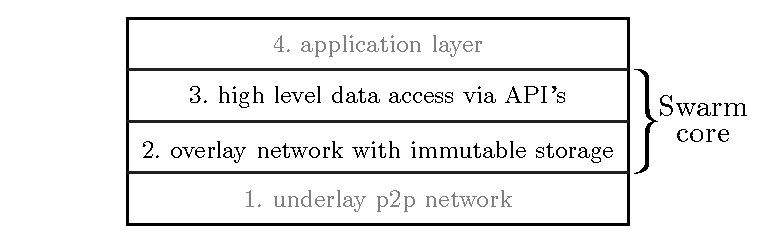
\includegraphics[width=0.8\textwidth]{fig/swarm-layered-design.pdf}
  \caption[Swarm's layered design \statusgreen]{Swarm's layered design}
\label{fig:Swarm-layered-design}
\end{figure}

This part details the design and architecture of the system. In accordance with the principles laid out in \ref{sec:design-principles}, we put an emphasis on modular design, and conceive of Swarm as having clearly separable layers, each dependent on the previous one (see figure \ref{fig:Swarm-layered-design}):

\begin{itemize}
\item (1) \emph{a peer-to-peer network protocol to serve as underlay transport,}
\item (2) \emph{an overlay network with protocols powering a distributed immutable storage of \glossplural{chunk} (fixed size data blocks),}
\item (3) \emph{a component providing high-level data access and defining APIs for base-layer features, and}
\item (4) \emph{an application layer defining standards, and outlining best practices for more elaborate use-cases.}
\end{itemize}

We regard (2) and (3) as the core of Swarm. Since the network layer relies on it, we will formulate also the requirements for (1), but we consider the detailed treatment of both (1) and (4) outside the scope of this book.


Central to the design, the architecture of Swarm overlay network (layer 2 in figure \ref{fig:Swarm-layered-design}) is discussed in chapter \ref{sec:network} and complemented by chapter \ref{sec:incentivisation}, describing the system of economic incentives which makes Swarm self-sustaining. In chapter \ref{sec:high-level-functionality}, we introduce the algorithms and conventions that allow Swarm to map data concepts on to the chunk layer to enable the high-level functionalities for storage and communication, notably data structures such as filesystems and databases, \gloss{access control}, indexed \gloss{feeds} and direct messaging  which comprise layer 3 of Swarm.
In chapter \ref{sec:persistence}, we present ways to prevent garbage collected chunks from disappearing from the network, including: \glossplural{erasure code}, \gloss{pinning} and insurance, and also provide ways to monitor, recover and re-upload them using missing chunk notifications and insurance challenges. 
Finally, in chapter \ref{sec:ux} we will look at functionality from a user experience perspective.

\chapter{Network}\label{sec:network}

This chapter offers a narrative on how the Swarm overlay network is built on top of a \gloss{peer-to-peer} network protocol to form a topology that allows for routing of messages between nodes (\ref{sec:topology-routing}). In \ref{sec:kademlia-storage}, we describe how such a network can serve as a scalable \gloss{distributed storage} solution for data chunks (\ref{sec:chunks}) and present the logic underpinning the protocols for retrieval/download and syncing/upload (\ref{sec:push-and-pull}).

\section{Topology and routing \statusgreen}\label{sec:topology-routing}

This section sets the scene (\ref{sec:underlay-transport}) for the \gloss{overlay network} (layer 2) of Swarm by making explicit the assumptions about the underlay network (layer 1). \ref{sec:overlay-addressing} introduces the \gloss{overlay address space} and explains how nodes are assigned an address. In  \ref{sec:kademlia-routing}, we present the \gloss{Kademlia} \gloss{overlay topology} (connectivity pattern) and explain how it solves routing between nodes. In \ref{sec:bootstrapping} we show how nodes running the Swarm client can discover each other, bootstrap and then maintain the overlay topology.

\subsection{Requirements for underlay network \statusyellow}\label{sec:underlay-transport} 

\yellow{}

Swarm is a network operated by its users. Each node in the network is supposed to run a client complying with the protocol specifications. On the lowest level, the nodes in the network connect using a peer-to-peer network protocol as their transport layer. This is called the \gloss{underlay network}. 
In its overall design, Swarm is agnostic of the particular underlay transport used as long as it satisfies the following requirements.

\begin{enumerate}
    \item \emph{addressing} -- Nodes are identified by their \gloss{underlay address}.
    \item \emph{dialling} -- Nodes can initiate a direct connection to a peer by dialing them on their underlay address.
    \item \emph{listening} -- Nodes can listen to other peers dialing them and can accept incoming connections. Nodes that do not accept incoming connections are called \glossplural{light node}.
    \item \emph{live connection} -- A node connection establishes a channel of communication which is kept alive until explicit disconnection, so that the existence of a connection means the remote peer is online and accepting messages.
    \item \emph{channel security} -- 
    The channel provides identity verification and implements encrypted and authenticated transport resisting man in the middle attacks.
    \item \emph{protocol multiplexing} -- 
    The underlay network service can accommodate several protocols running on the same connection. Peers communicate the protocols with the name and versions that they implement and the underlay service identifies compatible protocols and starts up peer connections on each matched protocol. 
    \item \emph{delivery guarantees} -- 
    Protocol messages have \gloss{guaranteed delivery}, i.e. delivery failures due to network problems result in direct error response. 
    Order of delivery of messages within each protocol is guaranteed. 
    Ideally the underlay protocol provides prioritisation. 
    If protocol multiplexing is over the same transport channel, this most likely implies framing, so that long messages do not block higher priority messages.
    \item \emph{serialisation} -- 
    The protocol message construction supports arbitrary data structure serialisation conventions.
    
\end{enumerate}

The \gloss{libp2p} library can provide all the needed functionality and is the one given in the specification as underlay connectivity driver, see \ref{spec:protocol:intro}.%
%
\footnote{Swarm's current golang implementation uses Ethereum's \gloss{devp2p}/rlpx which satisfies the above criteria and uses TCP/IP with custom cryptography added for security. The underlay network address devp2p uses is represented using the \gloss{enode URL scheme}. Devp2p dispatches protocol messages based on their message ID. It uses RLP serialisation which is extended with higher level data type representation conventions. In order to provide support for Ethereum 1.x blockchain and state on Swarm, we may provide a thin devp2p node that proxies queries to a libp2p-based Swarm client or just uses its API. Otherwise we expect the devp2p networking support to be discontinued.}

\subsection{Overlay addressing\statusgreen}\label{sec:overlay-addressing} 
\green{}

While clients use the \gloss{underlay address} to establish connections to peers, each node running Swarm is additionally identified with an \gloss{overlay address}. It is this address that determines which peers a node will connect to and directs the way that messages are forwarded. The overlay address is assumed to be stable as it defines a nodes' identity across sessions and ultimately affects which content is most worth storing in the nodes' local storage.

The node's \gloss{overlay address} is derived from an Ethereum account by hashing the corresponding elliptic curve public key with the \gloss{BZZ network ID}, using the 256-bit Keccak algorithm (see \ref{spec:format:bzzaddress}). The inclusion of the BZZ network ID stems from the fact that there can be many Swarm networks (e.g.\ test net, main net, or private Swarms). Including the BZZ network ID makes it impossible to use the same address across networks. Assuming any sample of base accounts independently selected, the resulting overlay addresses are expected to have a uniform distribution in the address space of 256-bit integers. This is important to deriving the address from a public key as it allows the nodes to issue commitments associated with an overlay location using cryptographic signatures which are verifiable by 3rd parties. 

Using the long-lived communication channels of the \gloss{underlay network}, Swarm nodes form a network with \emph{quasi-permanent} peer connections. The resulting connectivity graph can then realise a particular topology defined over the address space. The \gloss{overlay topology} chosen is called \gloss{Kademlia}: It enables communication between any two arbitrary nodes in the Swarm network by providing a strategy to relay messages using only underlay peer connections. The protocol that describes how nodes share information with each other about themselves and other peers, called 'Hive' is described in \ref{spec:protocol:hive}. How nodes use this protocol to bootstrap the \gloss{overlay topology} is discussed in \ref{sec:bootstrapping}. The  theoretical basis for \gloss{Kademlia topology} is formalised rigorously in \ref{sec:kademlia-connectivity}. 

Crucially, the overlay address space is all 256-bit integers. Central to Swarm is the concept of \gloss{proximity order} (\gloss{PO}), which quantifies the relatedness of two addresses on a discrete scale.%
%
\footnote{Proximity order is the discrete logarithmic scale of proximity, which, in turn is the inverse of normalised XOR distance. See \ref{sec:proximity} for a formal definition.}
%
Given two addresses, $x$ and $y$, $\mathit{PO}(x,y)$ counts the matching bits of their binary representation starting from the most significant bit up to the first one that differs. The highest proximity order is therefore 256, designating the maximum relatedness, i.e. where $x=y$.

\subsection{Kademlia routing \statusgreen}\label{sec:kademlia-routing}
\yellow{rework together with appendix}

\glossupper{Kademlia topology} can be used to route messages between nodes in a network using overlay addressing. It has excellent scalability as it allows for a universal routing such that both (1) the number of hops and (2) the number of peer connections are always logarithmic to the size of the network. 

In what follows, we show the two common flavours of routing: \emph{iterative/zooming} and \emph{recursive/forwarding}. Swarm's design crucially relies on choosing the latter, the forwarding flavour. However, this is unusual, and, as the iterative flavour predominates within much of the peer-to-peer literature and most other implementations are using iterative routing  (see \cite{maymounkov2002kademlia,baumgart2007s,lua2005survey}), we consider it useful to walk the reader through both approaches so their idiosyncrasies may be revealed.

\subsubsection{Iterative and forwarding Kademlia}

Let $R$ be an arbitrary binary relation over nodes in a network. Nodes that are in relation $R$ with a particular node $x$ are called \glossplural{peer} of $x$. Peers of $x$ can be indexed by their \gloss{proximity order} (\gloss{PO}) relative to $x$ (see \ref{sec:proximity}).
The equivalence classes of peers are called \glossplural{proximity order bin}, or just bins for short. Once arranged in bins, these groups of peers form the \gloss{Kademlia table} of the node $x$ (see figure \ref{fig:kademlia-table}). 



\begin{figure}[htbp]
   \centering
    % 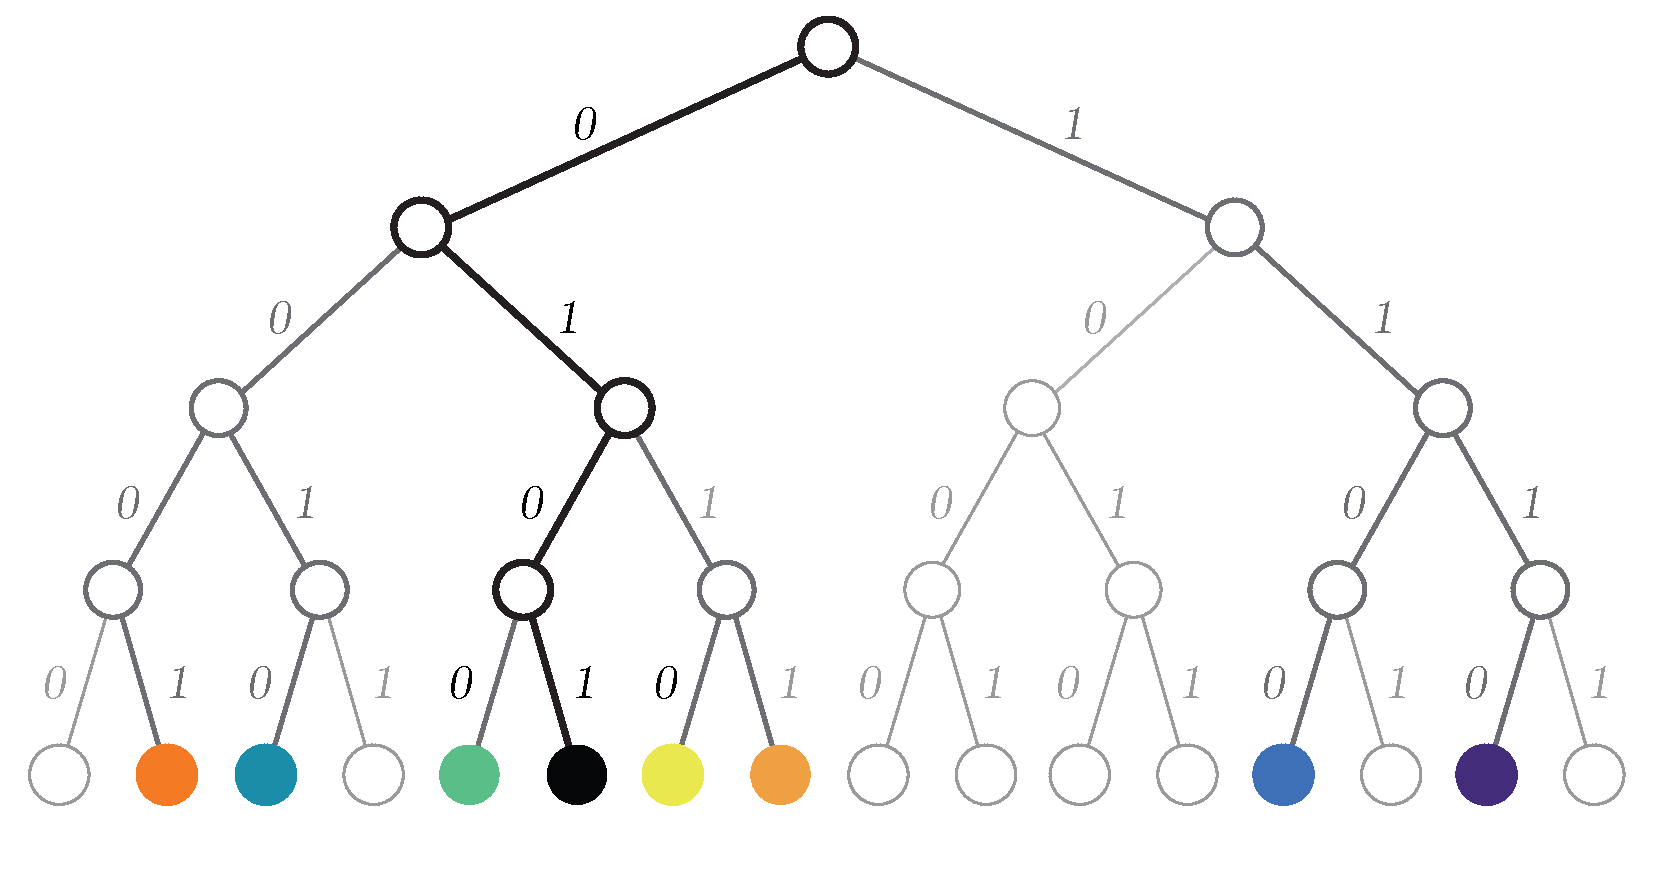
\includegraphics[width=0.7\textwidth]{fig/kademlia.pdf}
    % 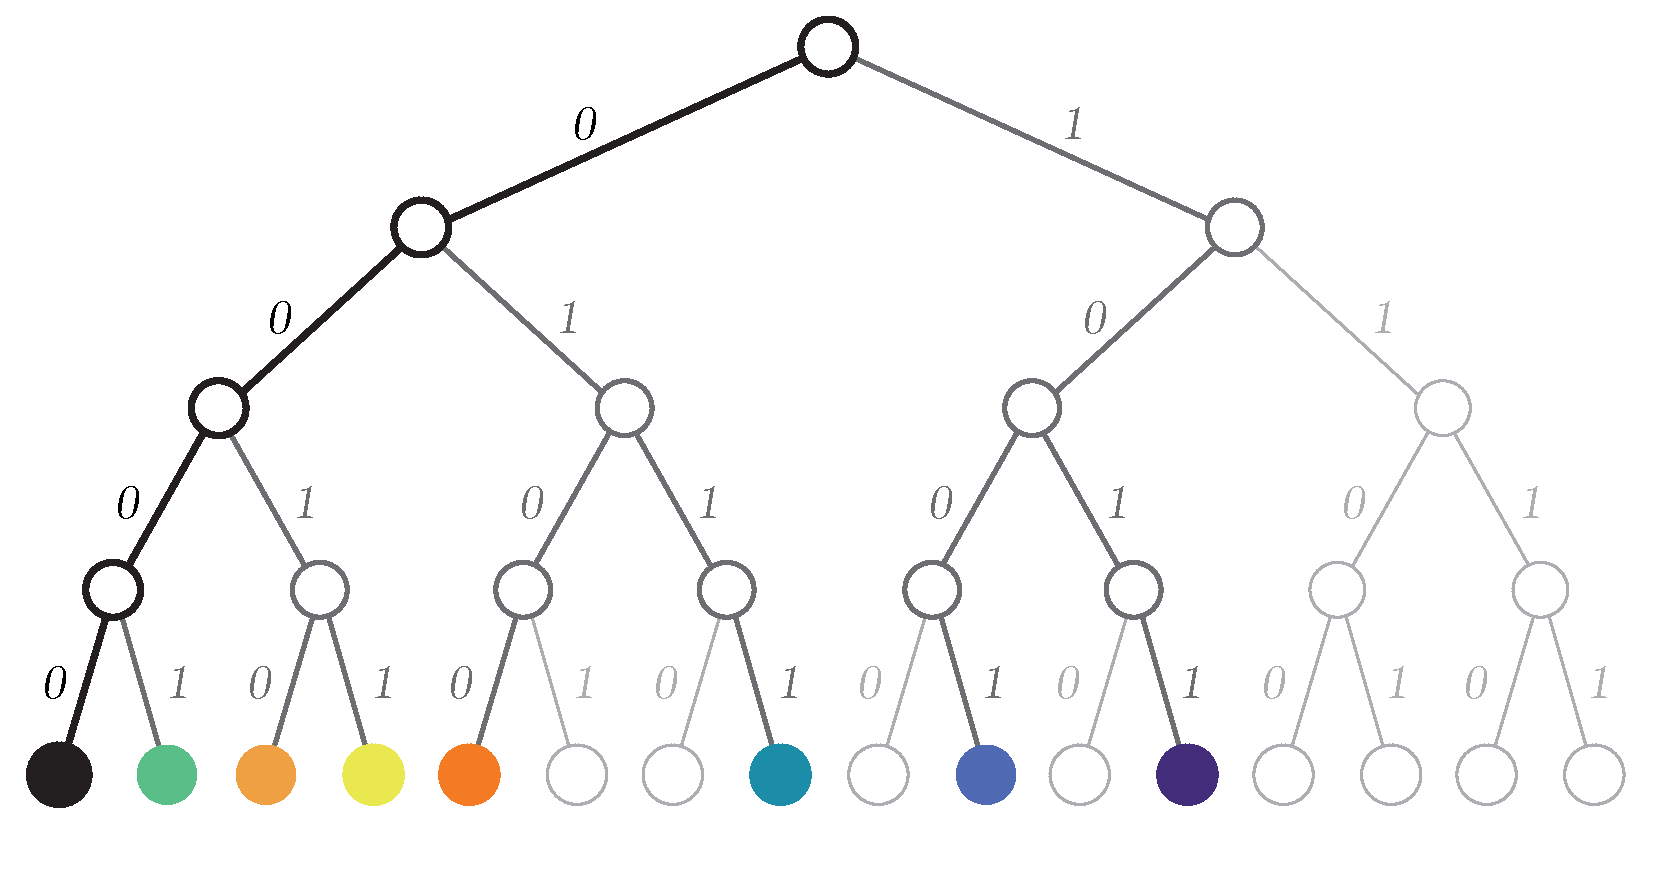
\includegraphics[width=0.7\textwidth]{fig/kademlia-2.pdf}
    % 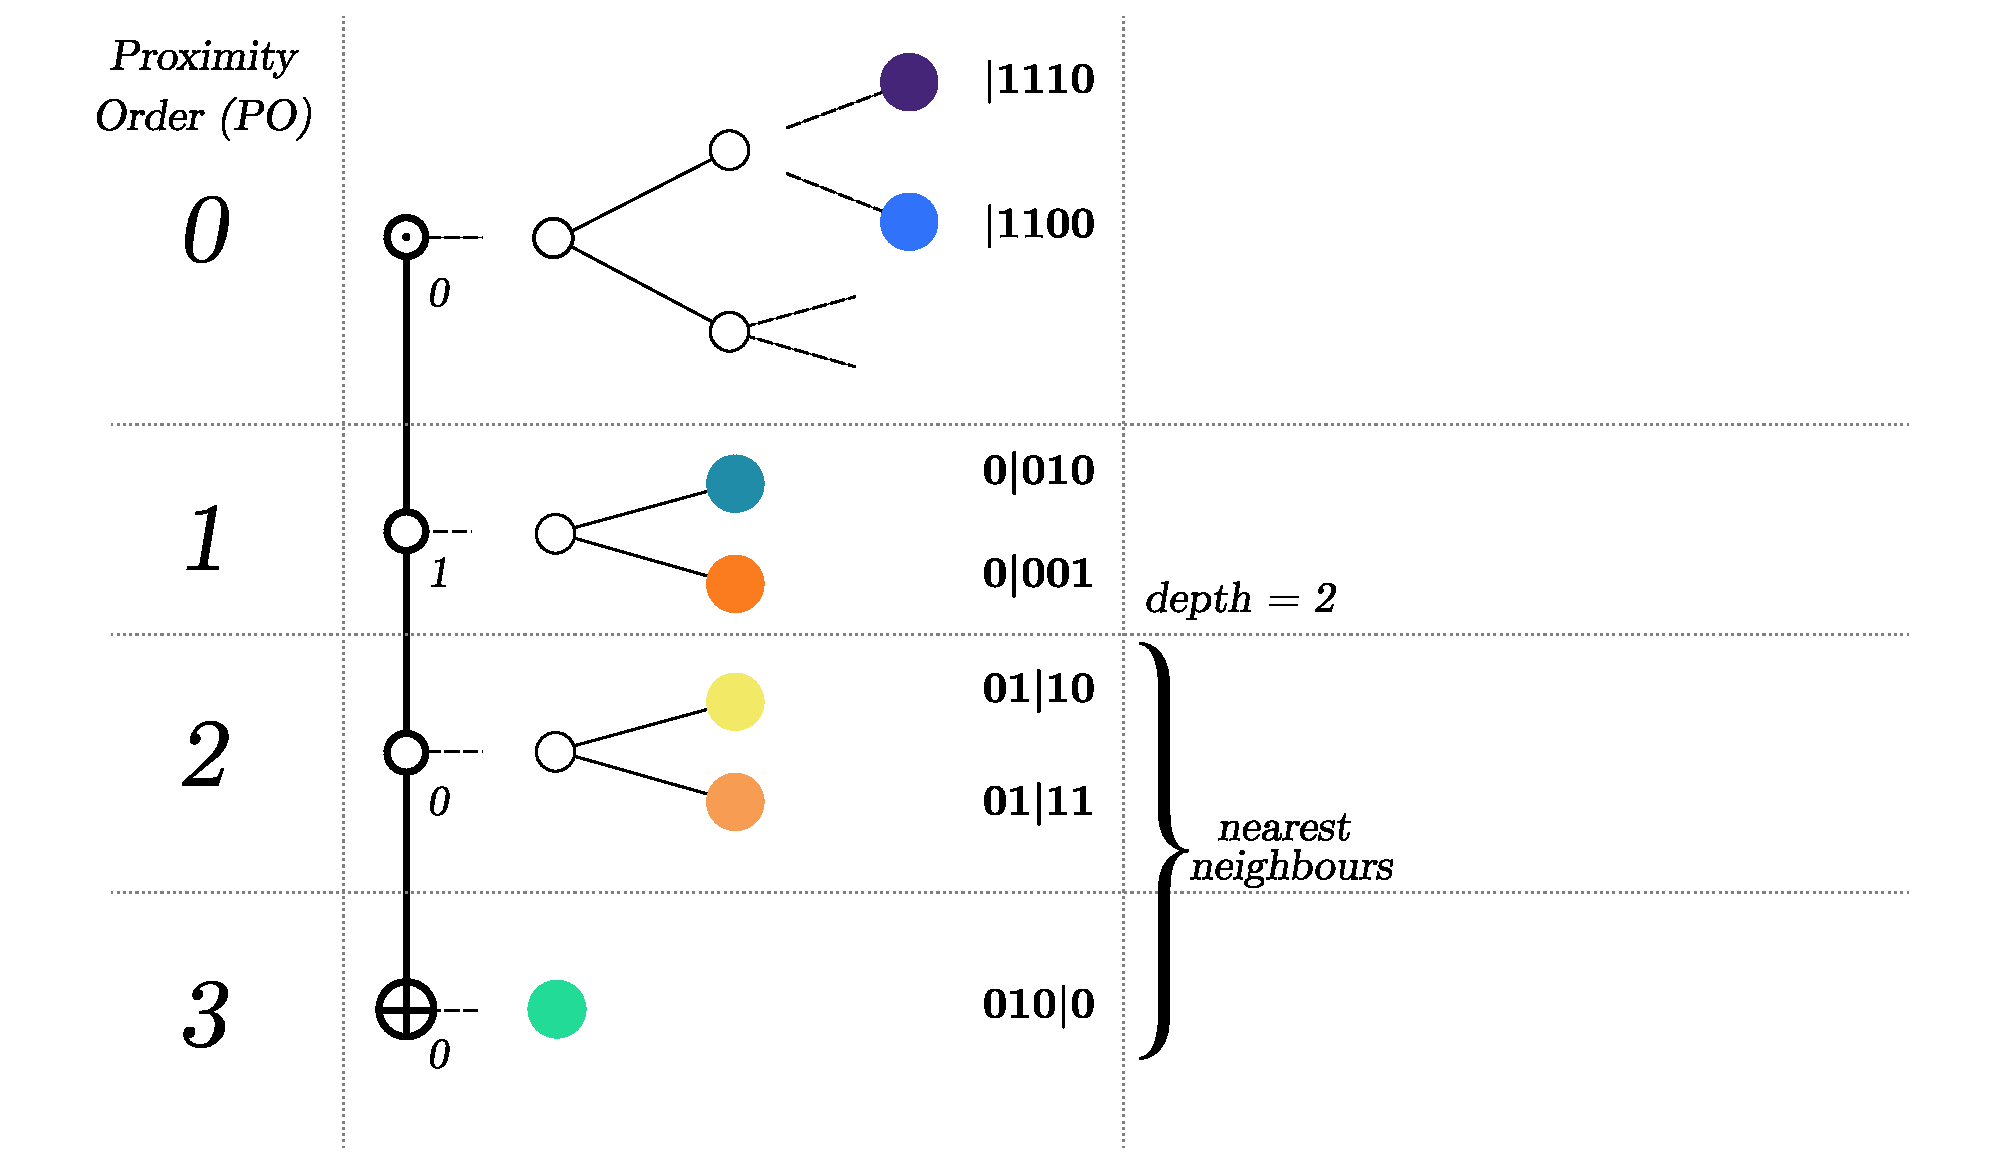
\includegraphics[width=0.8\textwidth]{fig/kademlia-3.pdf}
    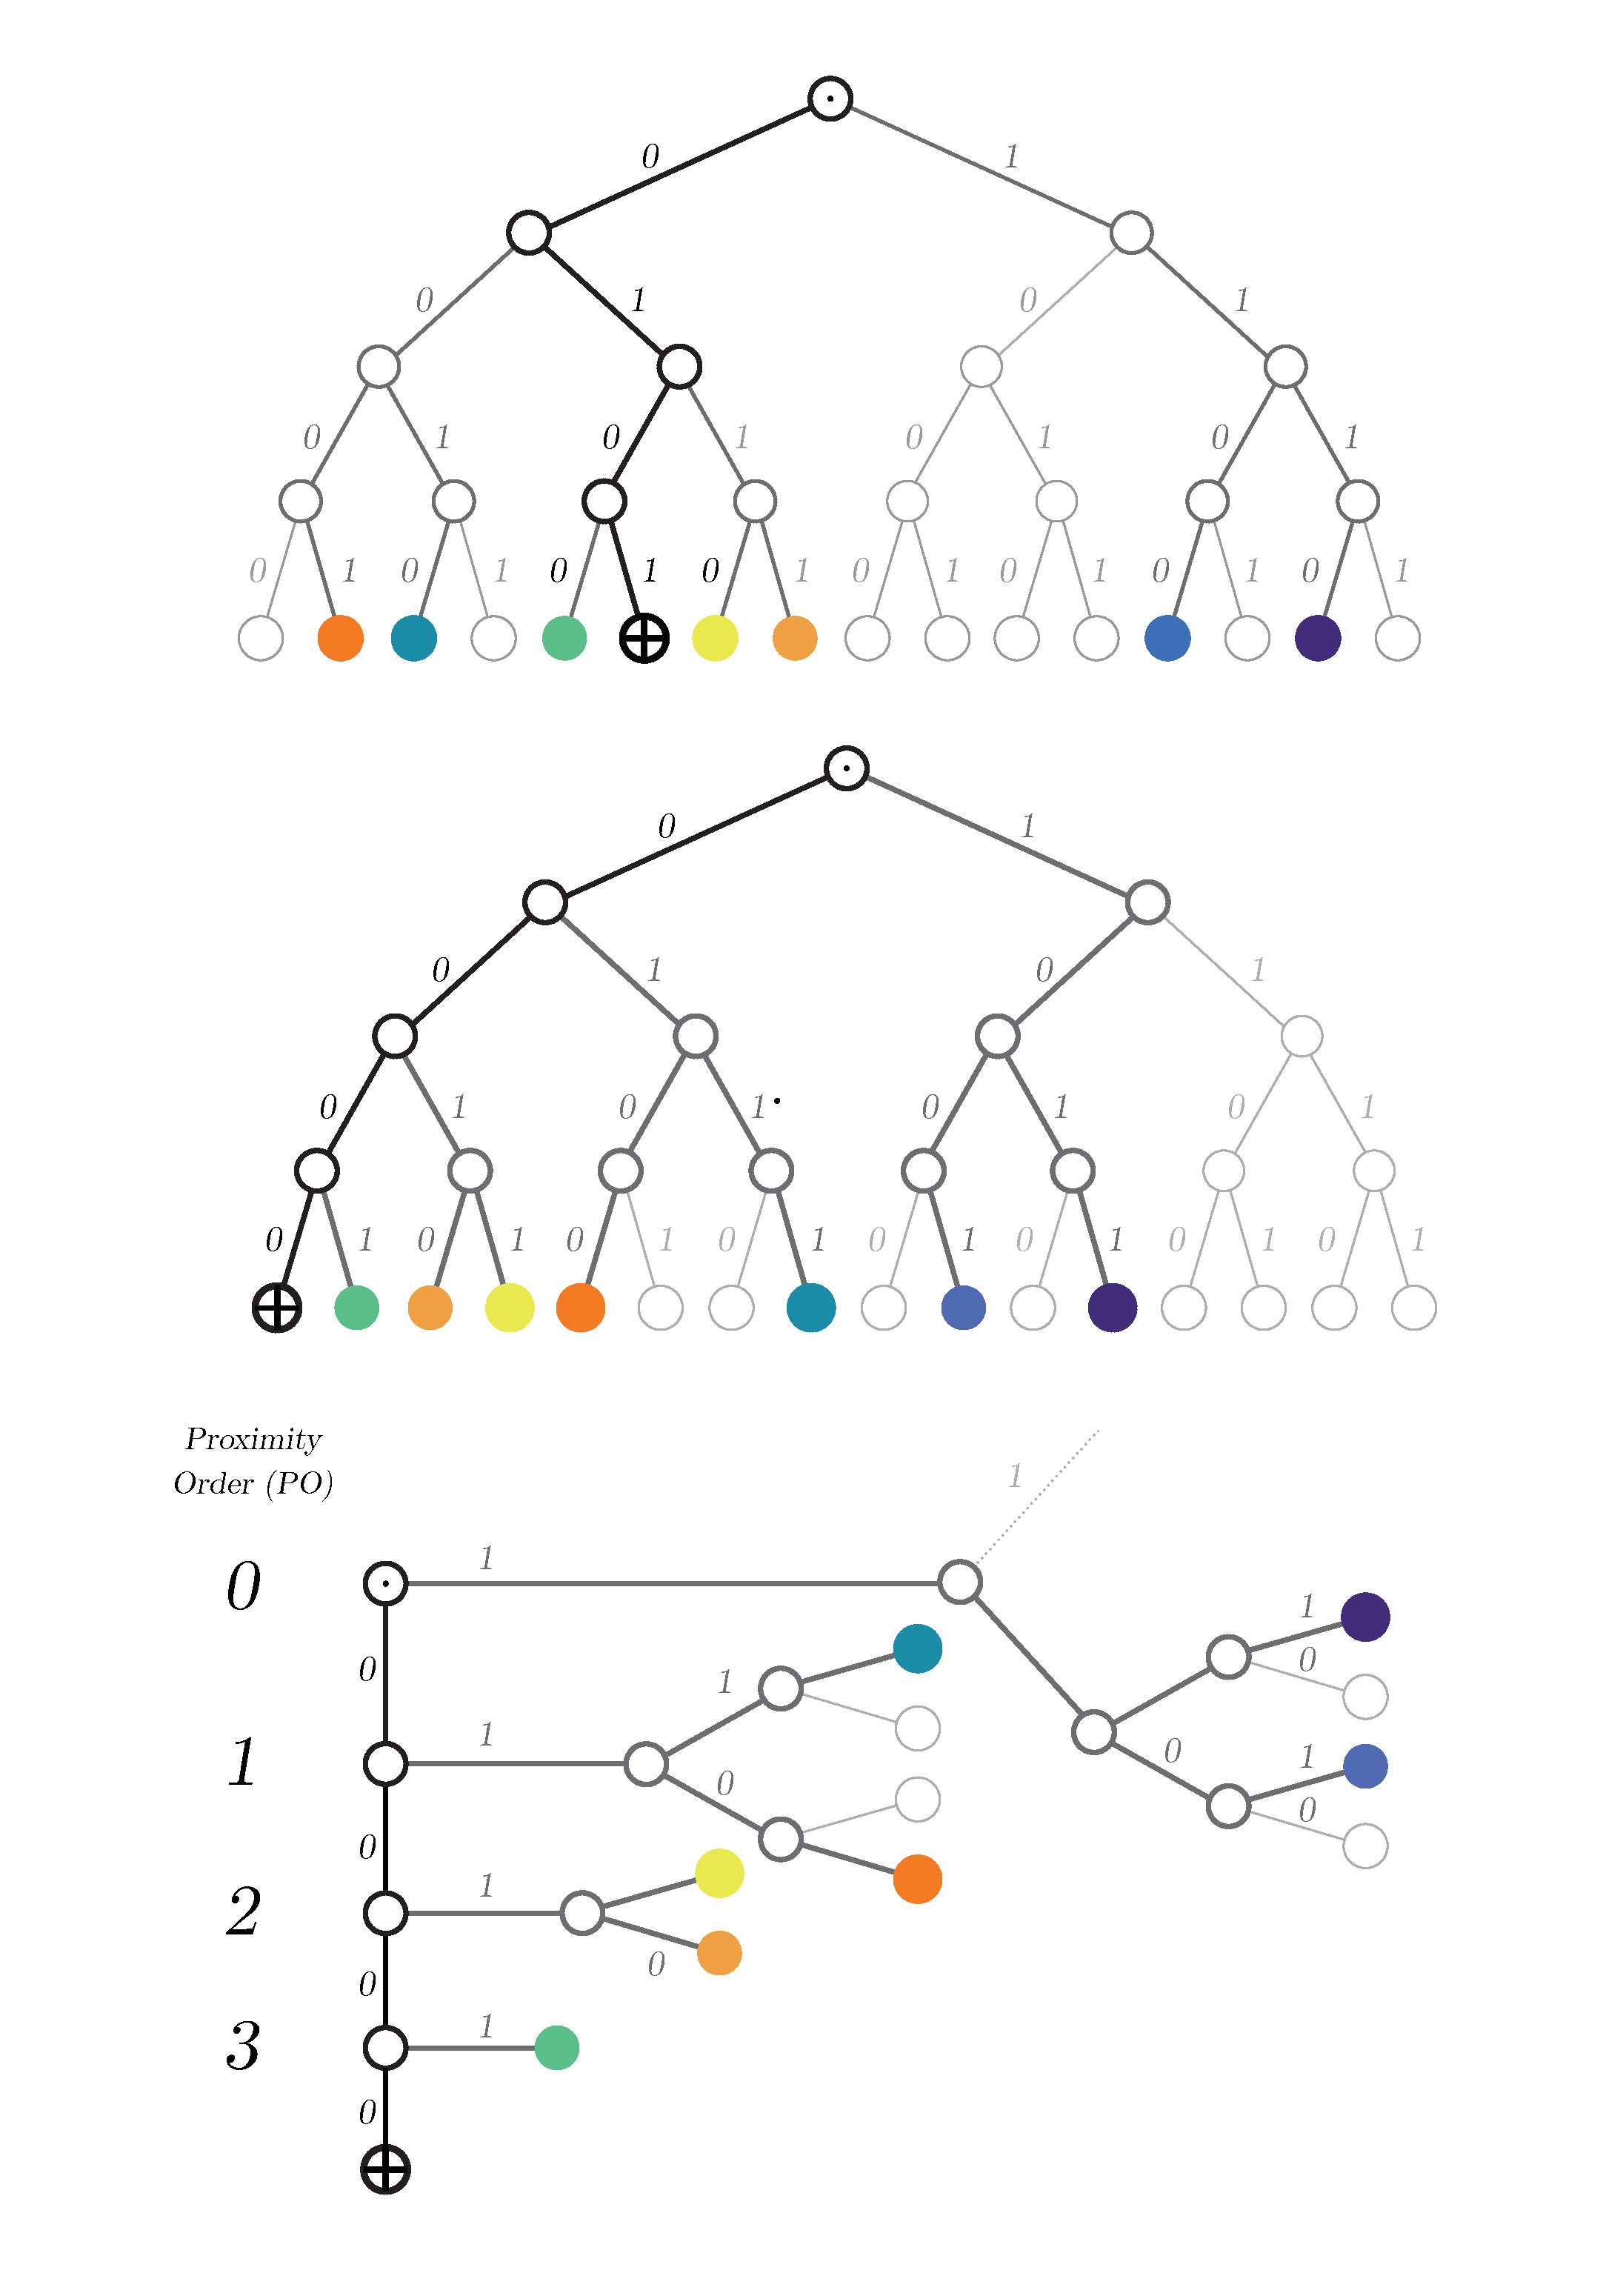
\includegraphics[width=.88\textwidth]{fig/kademlia-35.pdf}
   \caption[From overlay address space to Kademlia table \statusgreen]{From overlay address space to Kademlia table. \textbf{Top}: the overlay address space is represented with a binary tree, colored leaves are actual nodes. The path of the pivot node (+) is shown with thicker lines. \textbf{Centre}: peers of the pivot nodes are shown keyed by the bits of their xor distance measured from the pivot. Here zeros represent a matching bit with the pivot, ones show a differing bit. The leaf nodes are ordered by their xor distance from the pivot (leftmost node). \textbf{Bottom}: the Kademlia table of the pivot: the subtrees branching off from the pivot path on the left are displayed as the rows of the table representing proximity order bins in increasing order.}
   \label{fig:kademlia-table}
\end{figure}

Node $x$ has a \gloss{saturated Kademlia table} if there is a $0\leq d_x\leq \mathit{maxPO}$ called the  \gloss{neighbourhood depth} such that (1) the node has at least one peer in each bin up to and excluding \gloss{proximity order} bin $d_x$ and (2) all nodes at least as near as $d_x$ (called the \gloss{nearest neighbours}) are peers of $x$. If each node in a network has a saturated Kademlia table, then we say that the network has \gloss{Kademlia topology}.

\begin{figure}[htbp]
   \centering
    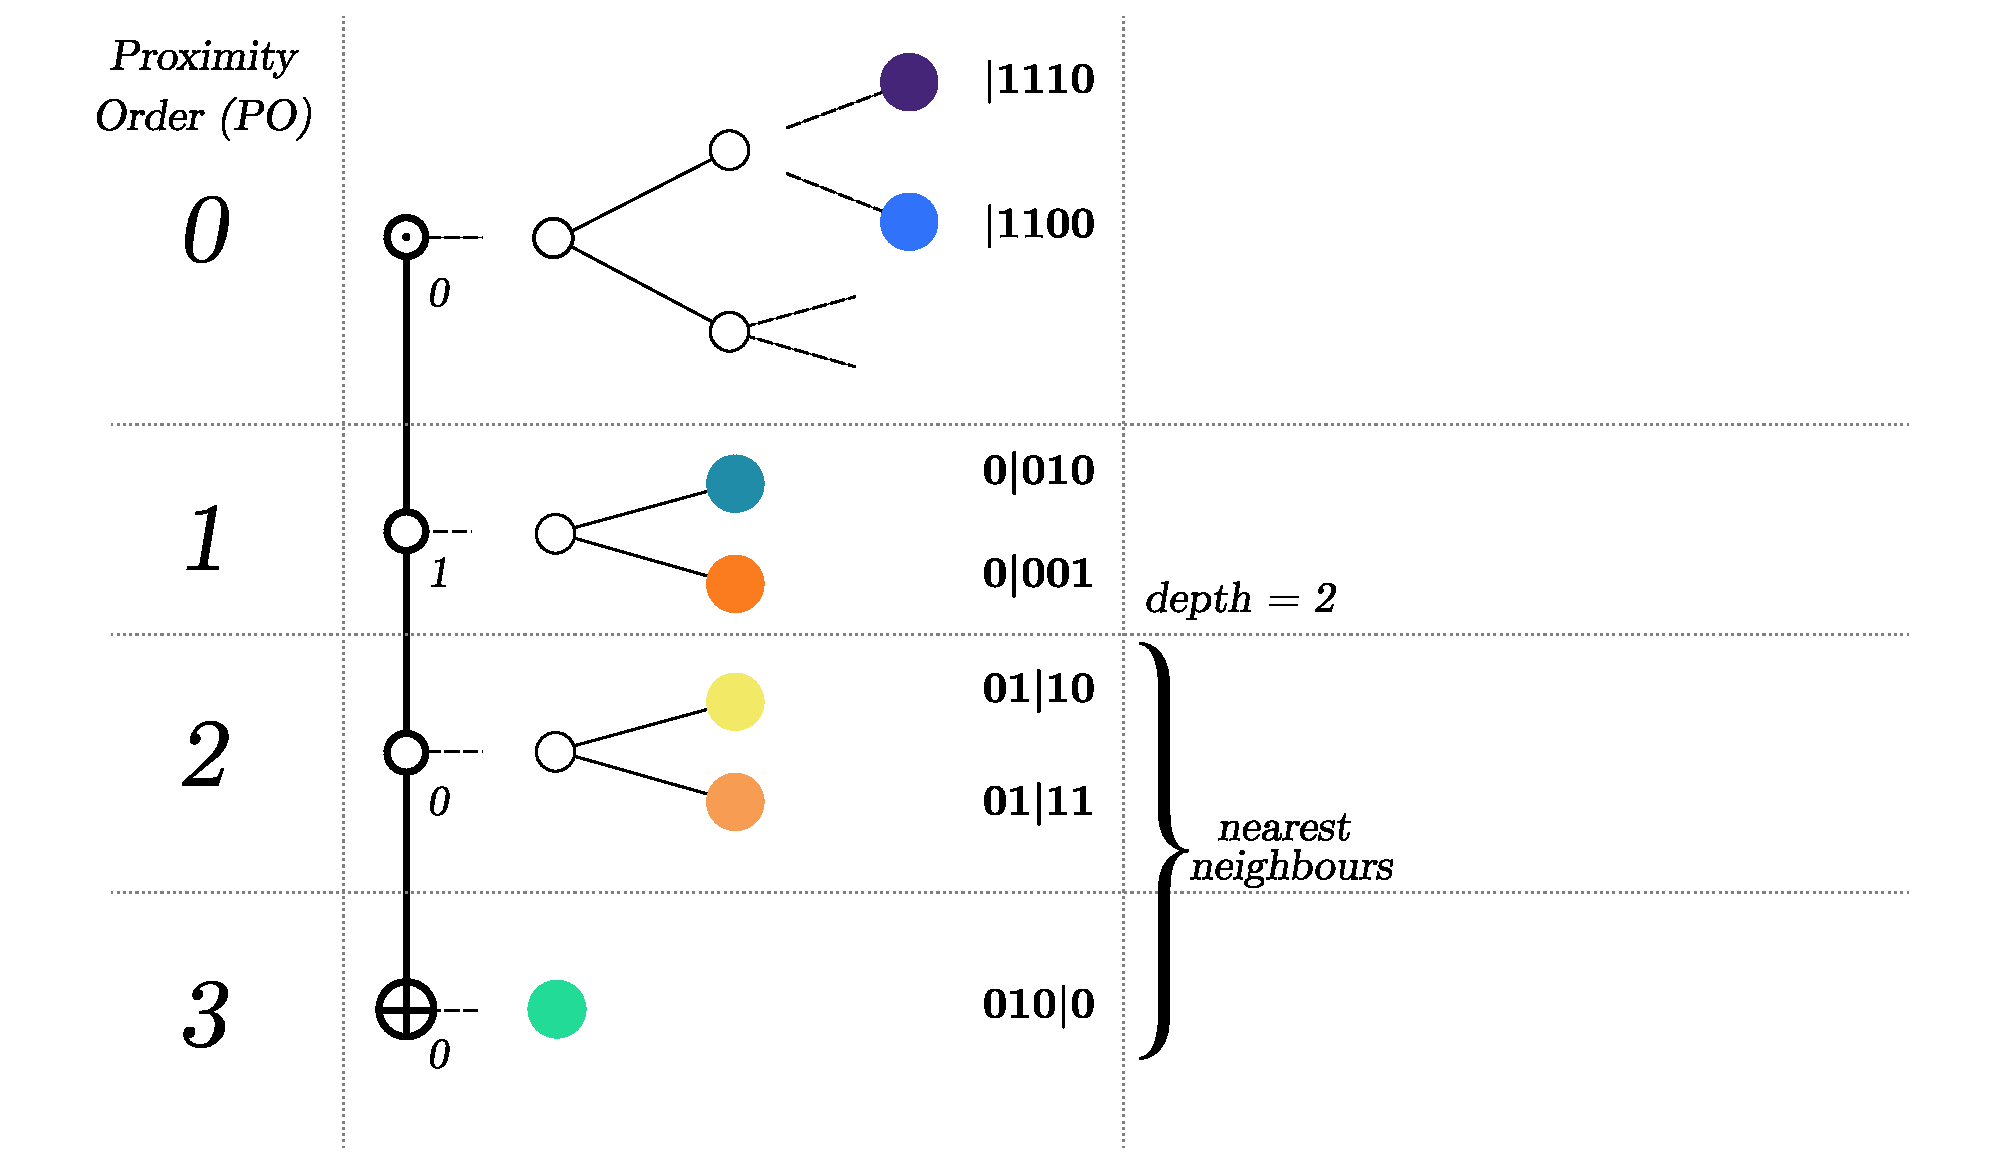
\includegraphics[width=\textwidth]{fig/kademlia-3.pdf}
   \caption[Nearest neighbours \statusgreen]{Nearest neighbours in a 4 bit network with $d = 2$ }
   \label{fig:bin-density}
\end{figure}

Let $R$ be the "is known to" relation:  $y$ "is known to" $x$ if $x$ has both overlay and underlay addressing information for $y$. 
In the iterative Kademlia routing the \gloss{requestor node} iteratively extends the graph of peers that are known to it. Using their \gloss{underlay address}, the requestor node will contact the peers that they know are nearest the destination address for peers that are further away (commonly using UDP), on each successive iteration the peers become at least one order closer to the destination (see figure \ref{fig:iterative-forwarding-kademlia}). Because of the Kademlia criteria, the requestor will end up eventually discovering the destination node's underlay address and can then establish direct communication with it. This iterative strategy%
%
\footnote{The iterative protocol is equivalent to the original Kademlia routing that is described in \cite{maymounkov2002kademlia}.
}
%
critically depends on the nodes' ability to find peers that are currently online. In order to find such a peer, a node needs to collect several candidates for each bin. The best predictor of availability is the recency of the peer's last response, so peers in a bin should be prioritised according to this ordering.

\begin{figure}[htbp]
   \centering
   \vspace{-2cm} 
   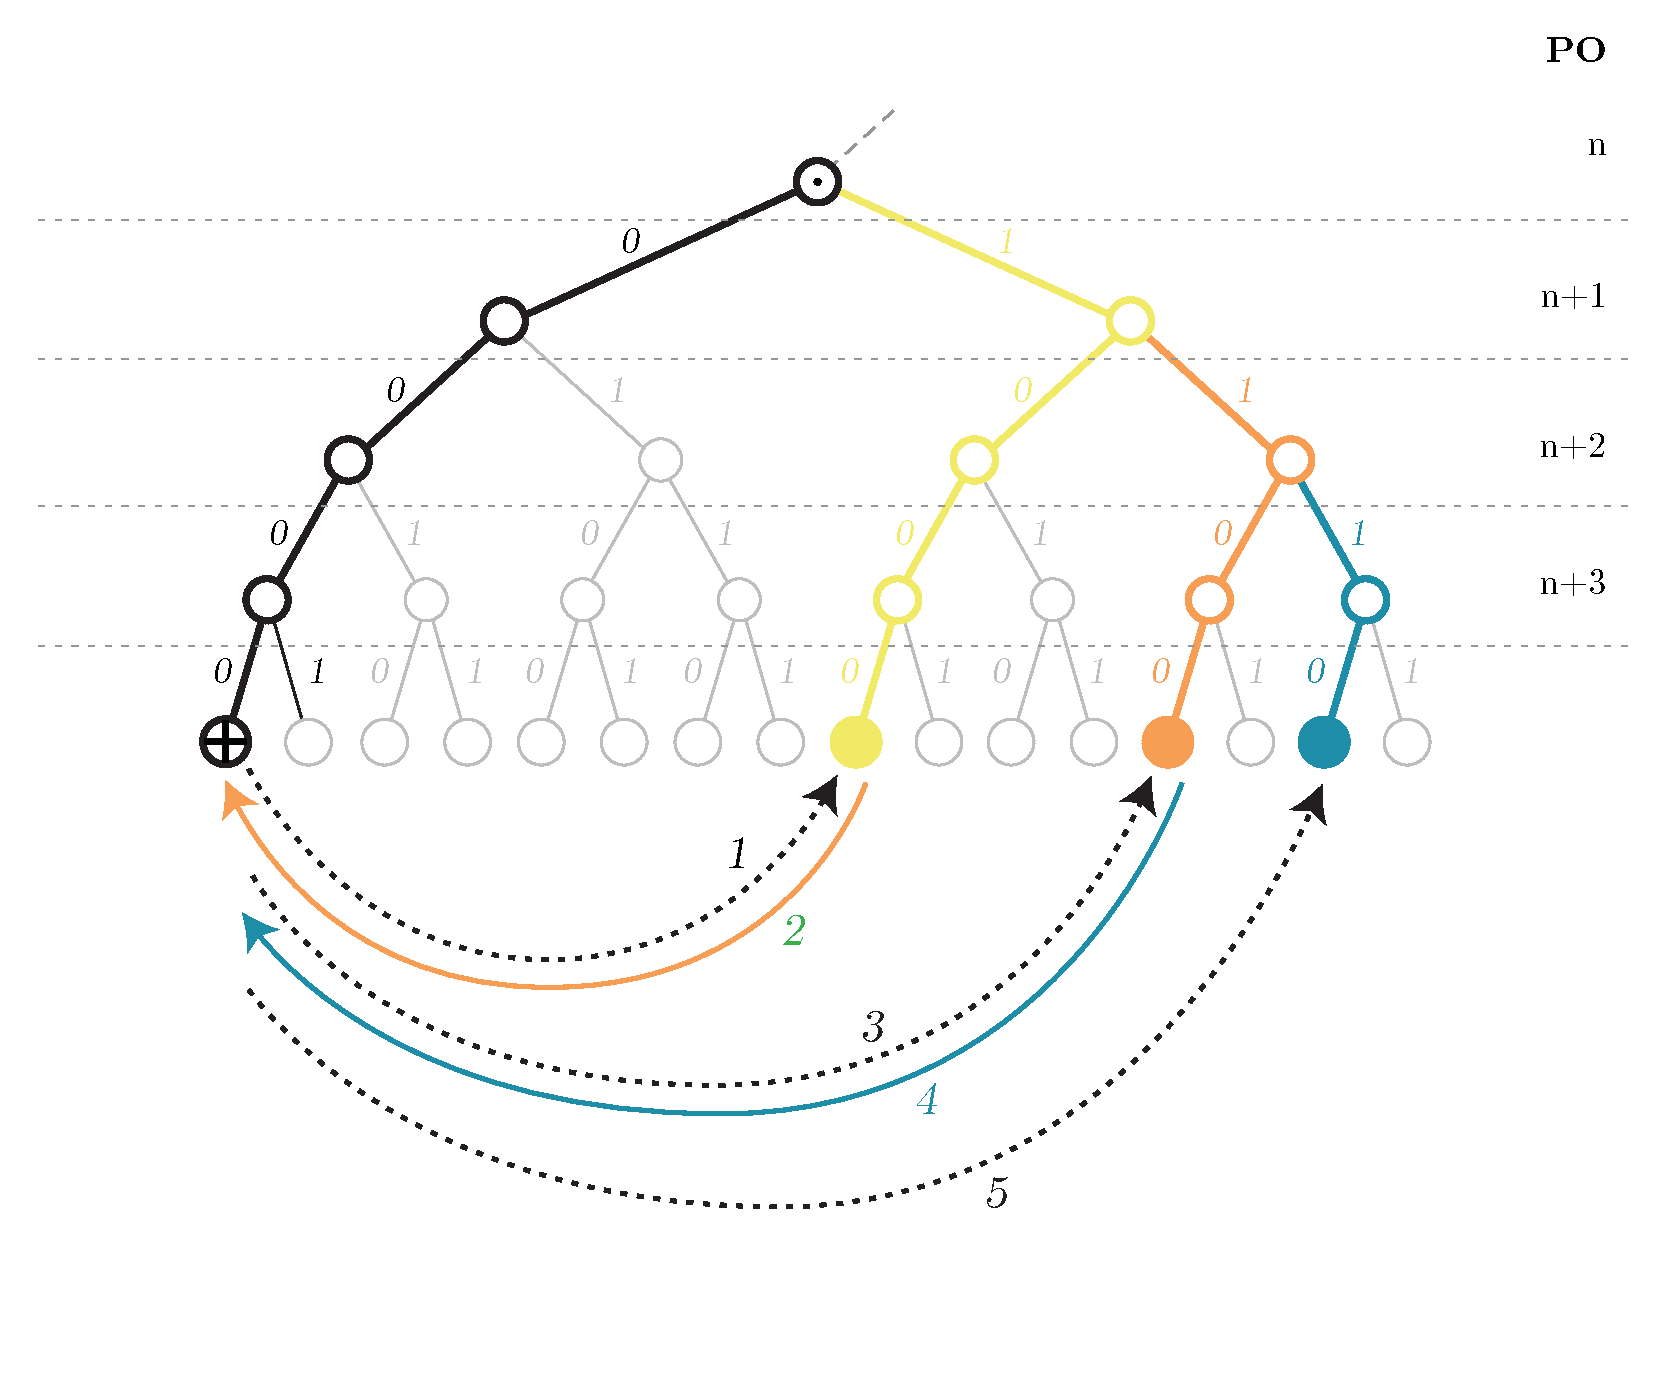
\includegraphics[width=.8\textwidth]{fig/iterative-kademlia.pdf}\\\vspace{-1.3cm}
   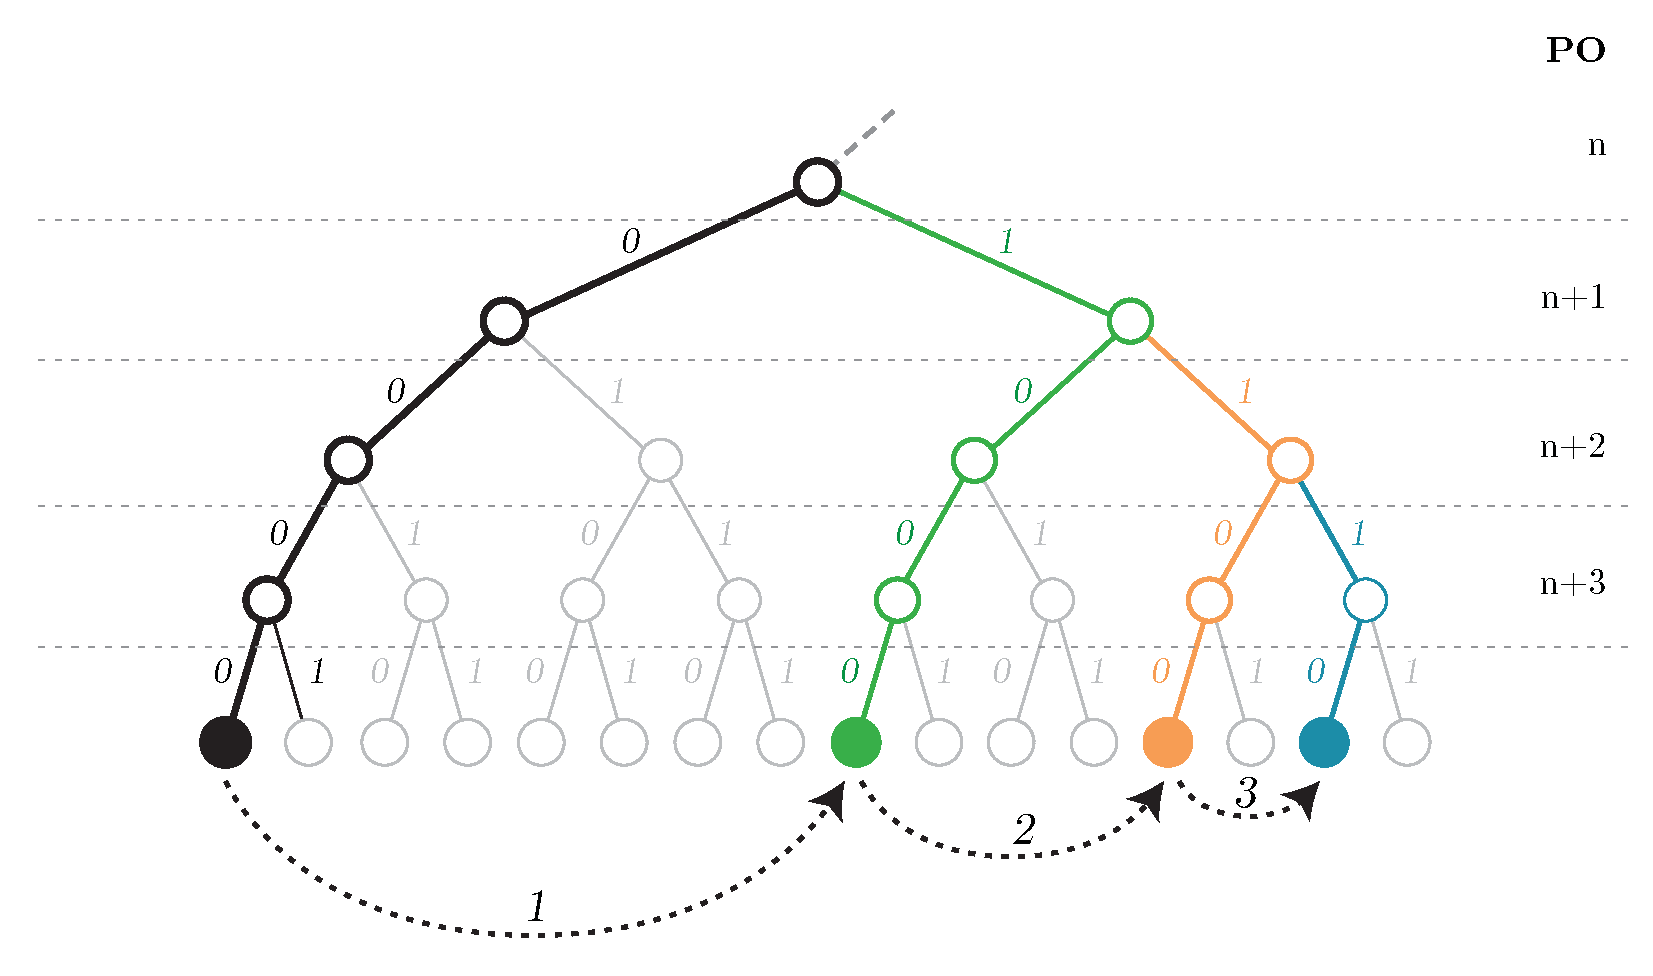
\includegraphics[width=.8\textwidth]{fig/forwarding-kademlia-3.pdf}
   \caption[Iterative and Forwarding Kademlia routing \statusgreen]{Iterative and Forwarding Kademlia routing: A requestor node shown with a cross in the circle at address $...0000...$ wants to route to a destination address $...1111...$ to which the closest peer online is the blue circle at $...1110...$ These initial ellipses represent the prefix shared by requestor and destination addresses which is $n$ bits long. \textbf{Top:} In the iterative flavour, the requestor contacts the peers (step 1, dotted black arrows) that they know are nearest the destination address. Peers that are online (yellow) respond with information about nodes that are even closer (green arrow, step 2) so the requestor can now repeat the query using these closer peers (green, step 3). On each successive iteration the peers (yellow, green and blue) are at least one PO closer to the destination until eventually the requestor is in direct contact with the node that is nearest to the destination address. \textbf{Bottom:} In the forwarding flavour, the requestor forwards a message to the connected peer they know that is nearest to the destination (yellow). The recipient peer does the same. Applying this strategy recursively relays the message via a chain of peers (yellow, green, blue) each at least one PO closer to the destination.}
   \label{fig:iterative-forwarding-kademlia}
\end{figure}


Swarm uses an alternative flavour of Kademlia routing which is first described in \cite{heep2010r} and then expanded on and worked out in \cite{tronetal2019-network}. Here, a recursive method is employed, whereby the successive steps of the iteration are "outsourced" to a \gloss{downstream peer}.
Each node recursively passes a message to a direct peer at least one \gloss{proximity order} closer to the destination. \glossupper{routing} here then means simply relaying messages via a chain of peers which are ever closer to the destination, as shown in figure \ref{fig:iterative-forwarding-kademlia}.


In this way, Swarm's underlay transport offers quasi-stable peer connections over TCP with communication channels that are kept alive. These open connections can then be used as $R$ to define another notion of a \gloss{peer}. The two criteria of healthy \gloss{Kademlia connectivity} in the swarm translate as: For each node $x$, there exists a \gloss{neighbourhood depth} $d_x$ such that (1) node $x$ has an open connection with at least one node for each \gloss{proximity order bin} up to but excluding $d_x$ and (2) is connected to all the online nodes that are at least as near as $d_x$. If each node in the network has a saturated Kademlia table of peers, then the network is said to have \gloss{Kademlia topology}. Since connected peers are guaranteed to be online, the recursive step consists solely of forwarding the message to a connected peer strictly closer to the destination. We can call this alternative a \gloss{forwarding Kademlia}.


In a \gloss{forwarding Kademlia} network, a message is said to be \emph{routable} if there exists a path from sender to destination through which the message can be relayed. In a mature subnetwork with \gloss{Kademlia topology} every message is routable. 

If all peer connections are stably online, a \gloss{thin Kademlia table}, i.e.\ a single \gloss{peer} for each bin up to $d$, is sufficient to guarantee routing between nodes. In reality, however, networks are subject to \gloss{churn}, i.e.\ nodes may be expected to go offline regularly. In order to ensure \gloss{routability} in the face of churn, the network needs to maintain \gloss{Kademlia topology}. This means that each individual node needs to have a \gloss{saturated Kademlia table} at all times. By keeping several connected peers in each \gloss{proximity order bin}, a node can ensure that node dropouts do not damage the saturation of their Kademlia table. Given a model of node dropouts, we can calculate the minimum number of peers needed per bin to guarantee that nodes are saturated with a probability that is arbitrarily close to 1. The more peers a node keeps in a particular proximity order bin, the more likely that the message destination address and the peer will have a longer matching prefix. As a consequence of forwarding the message to that peer, the \gloss{proximity order} increases more quickly, and the message ends up closer to the destination than it would with less peers in each bin (see also figure \ref{fig:bindensity}).



With \gloss{Kademlia} saturation guaranteed, a node will always be able to forward a message and ensure \gloss{routability}. If nodes comply with the forwarding principles (and that is ensured by \gloss{aligned incentives}, see \ref{spec:strategy:forwarding}) the only case when relaying could possibly break down is when a node drops out of the network after having received a message but before it has had chance to forward it.%
%
\footnote{Healthy nodes could commit to being able to forward within a (very short) constant time we can call the \gloss{forwarding lag}. In the case that a \gloss{downstream peer} disconnects before this forwarding lag passes, then the \gloss{upstream peer} can re-forward the message to an alternative peer, thereby keeping the message passing unbroken. See \ref{sec:retrieval} for more detail.
} 

An important advantage of forwarding Kademlia is that this method of routing requires a lot less bandwidth than the iterative algorithm. In the iterative version, known peers are not guaranteed to be online, so finding one that is adds an additional level of unpredictability.

\subsubsection{Sender anonymity}
\glossupper{sender anonymity} is a crucial feature of  Swarm. It is important that since requests are relayed from peer-to-peer, those peers further down in the request cascade can never know who the originator of the request was. 

The above rigid formulation of Kademlia routing would suggest that if a node receives a message from a peer and that message and peer have a proximity order of $0$, then the recipient would be able to conclude that the peer it received the message from must be the sender. If we allow \gloss{light node} Swarm clients who, since they are running in a low-resource environment, do not keep a full Kademlia saturation but instead have just a local neighbourhood, even a message from a peer in bin $0$ remains of ambiguous origin. 

\subsubsection{Bin density and multi-order hops} \label{sec:bindensity}

As a consequence of logarithmic distance and uniform node distribution, farther peers of a particular node are exponentially more numerous. 
As long as the number of connected peers is less than double the number in the bin one closer, then shallower bins will always allow more choice for nodes. In particular, nodes have a chance to increase the number of connections per bin in such a way that peer addresses maximise density (in proximity order bin $b$, the subsequent bits of peers addresses form a \gloss{balanced binary tree}). Such an arrangement is optimal in the sense that for a bin depth of $d$, nodes are able to relay all messages so that in one hop, the proximity order of the destination address will increase by $d$ (see figure \ref{fig:bindensity}). 


\begin{figure}[htbp]
   \centering
   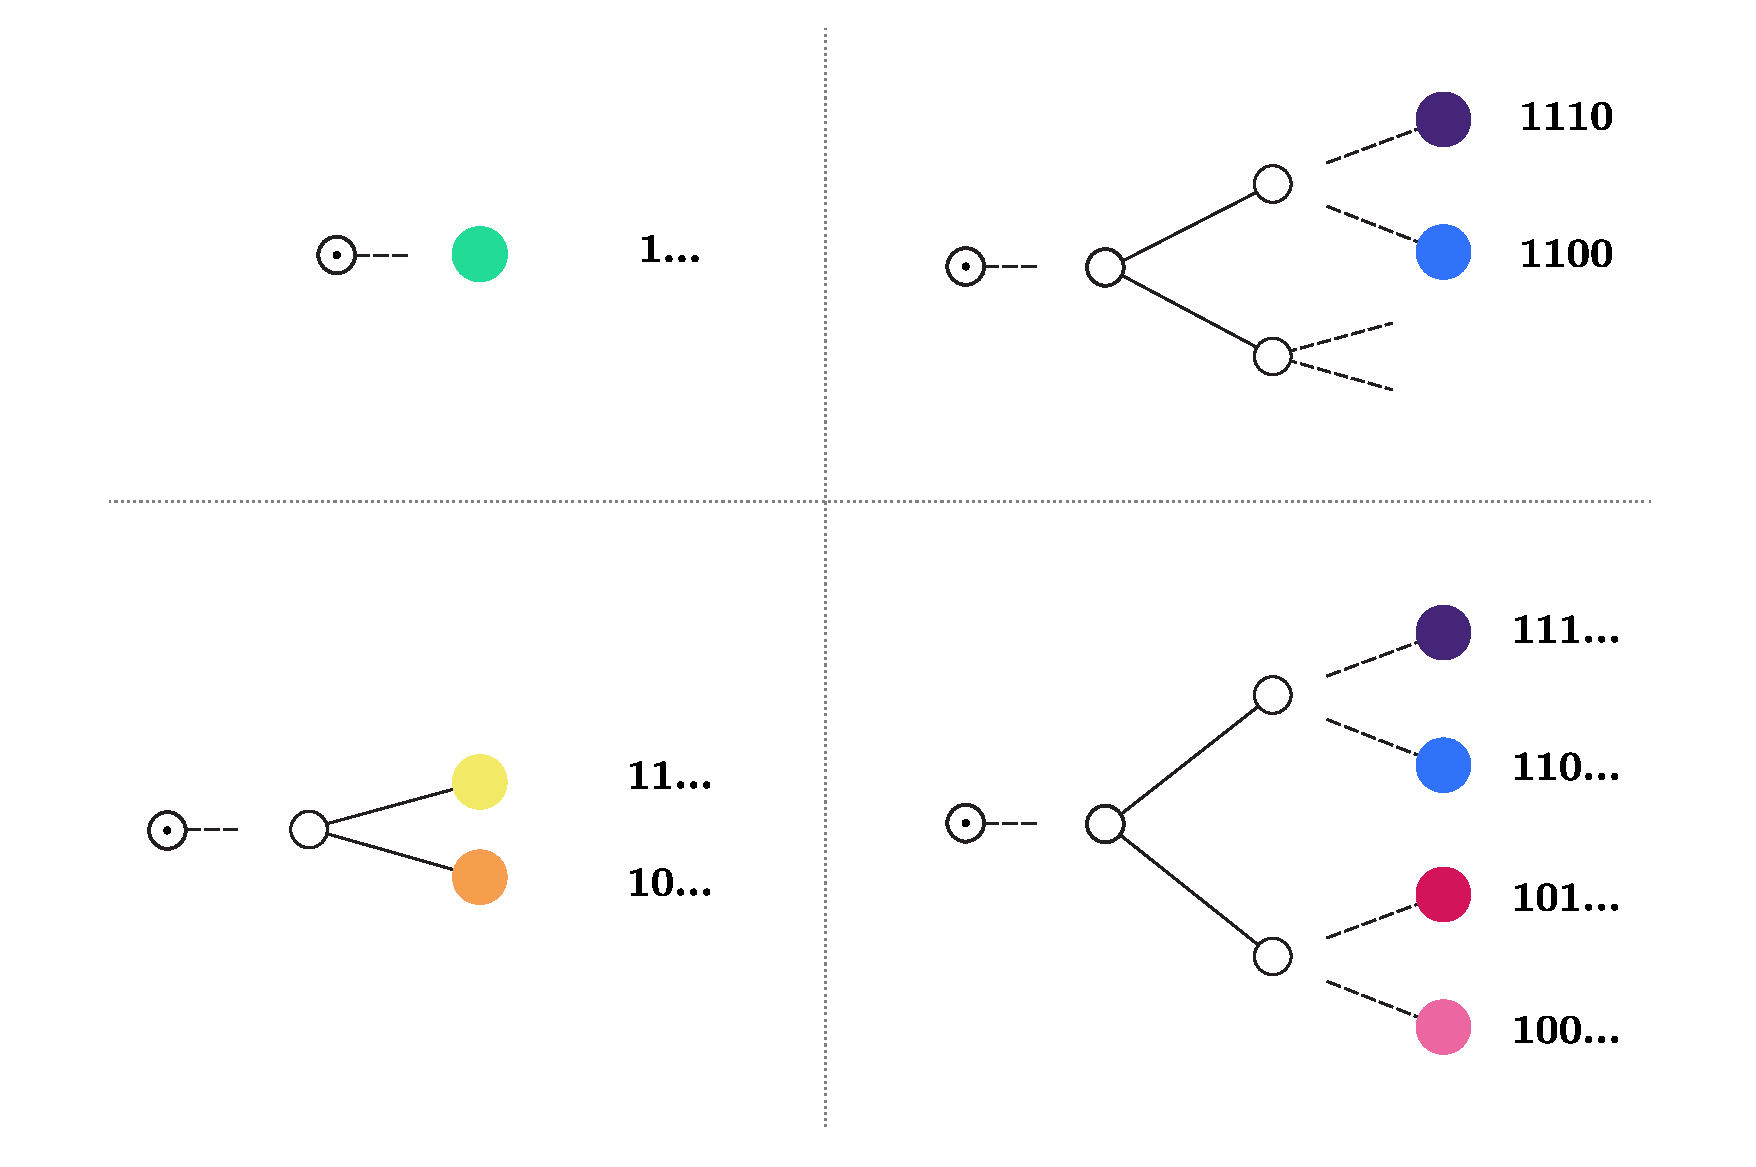
\includegraphics[width=\textwidth]{fig/bindensity.pdf}
   \caption[Bin density \statusgreen]{Bin density:  types of saturation for PO bin $0$ for a node with overlay address starting with bit $0$. \textbf{Top left}: A "thin" bin with a single peer is not resilient to churn and only increases PO by $1$ in one hop. \textbf{Top right:} At least two peers are needed to maintain Kademlia topology in case of churn; two peers when not balanced cannot guarantee multi-order hops. \textbf{Bottom left:} Two peers balanced guarantees an increase of 2 PO-s in one hop. \textbf{Bottom right:} Four peers when balanced can guarantee an increase of $3$ PO-s in one hop.}
   \label{fig:bindensity}
\end{figure}

\subsubsection{Factoring in underlay proximity}
It is expected that as Swarm clients continue to evolve and develop, nodes may factor in throughput when they select peers for connection. All things being equal, nodes in geographic physical proximity tend to have higher throughput, and therefore will be preferred in the long run. This is how forwarding Kademlia is implicitly aware of underlay topology \cite{heep2010r}. See \ref{spec:strategy:connection} for a more detailed discussion of connectivity strategy.


\subsection{Bootstrapping and maintaining Kademlia topology \statusgreen}\label{sec:bootstrapping}
 
\orange{rework based on new hive protocol}
 
This section discusses how a stable Kademlia topology can emerge. In particular, the exact bootstrapping protocol each node must follow to reach a saturated Kademlia connectivity and maintain it. Nodes joining a \gloss{decentralised network} are supposed to be initially naive, potentially initiating connection via only a single known peer with no prior knowledge. For this reason, the bootstrapping process needs to include a discovery component with the help of which nodes exchange information about each other. This protocol is called the \gloss{hive protocol} and is formally specified in \ref{spec:protocol:hive}.

\subsubsection{Bootnodes}

Swarm has no distinct node type or operation  mode for bootnodes. This means that naive nodes should be able to connect to any node on the  network and bootstrap their desired connectivity. In order not to overburden any single node, specifying a particular node as an initial connection should be avoided and the role of bootnode with respect to new naive nodes should ideally be balanced between participant nodes. This is achieved either with an invite system or a centralised bootnode service running a public gateway which responds to an API call with the bzz address of a randomly chosen node among online peers. 

Once connected to a node in the network, the hive protocol will kick in and the naive node will learn about the bzz addresses of other nodes and can start bootstrapping its connectivity.

\subsubsection{Building up connections}

Initially, each node begins with zero as their \gloss{saturation depth}. Nodes keep advertising their saturation depth to their connected peers as it changes. When a node $A$ receives an attempt to establish a new connection from a node $B$, she notifies each of her other peers of the node $B$ connecting to her only in the case that each peer's proximity order relative to the connecting node $A$ is not lower than that peer's advertised saturation depth. The notification is always sent to a peer that shares a proximity order bin with the new connection. Formally, when $x$ connects with a peer $y$, $x$ notifies each of her peers if $\mathit{PO}(x, p) = \mathit{PO}(x, y)$ or $d_p\leq \mathit{PO}(y, p)$. In particular, notification includes the full \gloss{overlay address} and \gloss{underlay address} information (see \ref{spec:format:bzzaddress}).%
%
\footnote{Light nodes that do not wish to relay messages and do not aspire to build up a healthy Kademlia, are not included, see section \ref{sec:light}. }

    

% \begin{figure}[htbp]
%   \centering
%   \caption[Hive protocol: bootstrapping and maintaining Kademlia topology \statusred]{Hive protocol: bootstrapping and maintaining Kademlia topology}
%   \label{fig:bootstrapping-kademlia}
% \end{figure}

\subsubsection{Mature connectivity}

After a sufficient number of nodes are connected, a bin becomes saturated, and the node's neighbourhood depth can begin to increase. Nodes keep their peers up to date by advertising their current depth if it changes. As their depth increases, nodes will get notified of fewer and fewer peers. Once the node finds all their nearest neighbours and has saturated all the bins, no new peers are to be expected. For this reason, a node can conclude a saturated Kademlia state if it receives no new peers for some time.%
%
\footnote{Although the node does not need to know the number of nodes in the network. In fact, some time after the node stops receiving new peer addresses, the node can effectively estimate the size of the network: the depth of network is $\log_2(n+1)+ d$ where $n$ is the number of remote peers in the nearest neighbourhood and $d$ is the depth of that neighbourhood. It then  follows that the total number of nodes in the network can be estimated simply by taking this the exponent of 2 .}
%
Instead of having a hard deadline and a binary state of saturation, we can quantify the certainty of saturation by the age of the last new peer received. Assuming stable connections, eventually each node online will get to know its nearest neighbours and connect to them while keeping each bin up to $d$ non-empty. Therefore each node will converge on the saturated state. If no new nodes join, health (Kademlia topology) is maintained even if peer connections change. A node is not supposed to go back to a lower saturation state for instance. This is achieved by requiring several peers in each proximity order bin. 

\section{Swarm storage\statusgreen}\label{sec:kademlia-storage}

In this section, we first show how a network with quasi-permanent connections in a Kademlia topology can support a \gloss{load balancing}, \gloss{distributed storage} of fixed-sized datablobs in \ref{sec:disc}. In \ref{sec:chunks}, we detail the generic requirements on chunks and introduce actual chunk types. Finally, in \ref{sec:redundancy-by-local-replication}, we turn to \gloss{redundancy} by neighbourhood replication as a fundamental measure for churn-resistance.

\subsection{Distributed immutable store for chunks\statusgreen}\label{sec:disc}
 
In this section we discuss how networks using Kademlia overlay routing are a suitable basis on which to implement  serverless storage solution using \glossplural{distributed hash table} (\glossplural{DHT}). Then we introduce the \gloss{DISC}%
%
\footnote{DISC is \gloss{distributed immutable store for chunks}. In earlier work, we have referred to this component as the 'distributed preimage archive' (DPA), however, this phrase became misleading since we now also allow chunks that are not the preimage of their address.}
% 
model, Swarm's narrower interpretation of a DHT for storage. This model 
imposes some requirements on chunks and necessitates 'upload' protocols. 

As is customary in Swarm, we provide a few resolutions of this acronym, which summarise the most important features:


\begin{itemize}
\item \emph{decentralised infrastructure for storage and communication}, 
\item \emph{distributed immutable store for chunks}, 
\item \emph{data integrity by signature or content address},
% \item \emph{downloadable incentivised secure communications}
\item \emph{driven by incentives with smart contracts}. 

\end{itemize}
 
\subsubsection{From DHT to DISC}
Swarm's \gloss{DISC} shares many similarities with the more familiar \glossplural{distributed hash table}. The most important difference is that Swarm does not keep a list of \emph{where} files are to be found, instead it actually \emph{stores pieces of the file itself} directly with the closest node(s). 
In what follows, we review DHTs, as well as dive into the similarities and differences with DISC in more detail. 
 
\glossupperplural{distributed hash table} use an overlay network to implement a key--value container distributed over the nodes (see figure \ref{fig:DHT}). The basic idea is that the keyspace is mapped on to the overlay address space, and the value for a key in the container is to be found with nodes whose addresses are in the proximity of the key. In the simplest case, let us say that this is the single closest node to the key that stores the value. In a network with Kademlia connectivity, any node can route to a node whose address is closest to the key, therefore a \emph{lookup} (i.e.\ looking up the value belonging to a key) is reduced simply to routing a request. 

\begin{figure}[htbp]
   \centering
   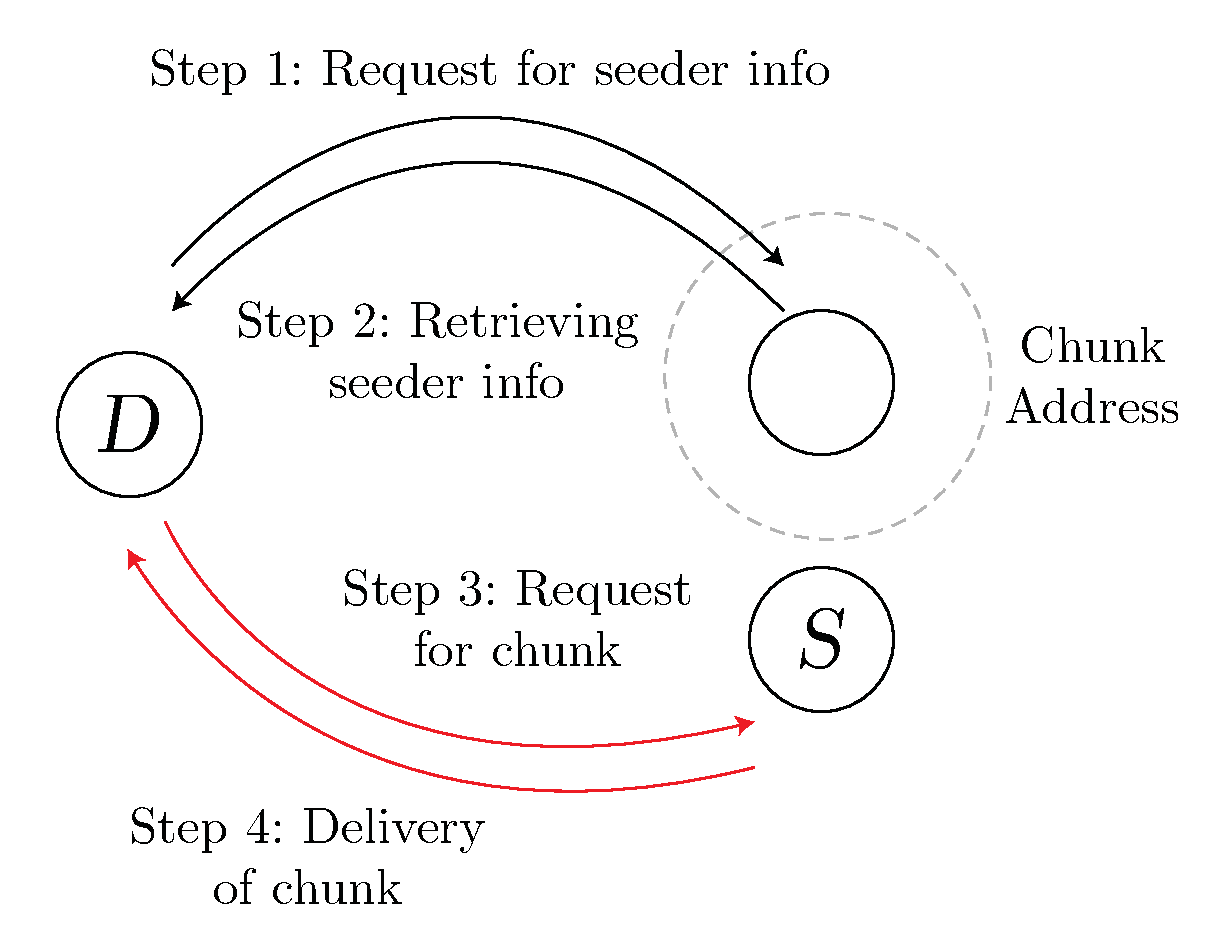
\includegraphics[width=0.7\textwidth]{fig/dht.pdf}
   \caption[Distributed hash tables (DHTs) \statusgreen]{Distributed hash tables (DHTs) used for storage:  node $D$ (downloader) uses Kademlia routing in step $1$ to query nodes in the neighbourhood of the chunk address to retrieve seeder info in step $2$. The seeder info is used to contact node $S$ (seeder) directly to request the chunk and deliver it in steps $3$ and $4$.}
   \label{fig:DHT}
\end{figure}

DHTs used for \gloss{distributed storage} typically associate content identifiers (as keys/addresses) with a changing list of seeders (as values) that can serve that content \cite{ipfs2014, crosby2007analysis}. However, the same structure can be used directly: in Swarm, it is not information about the location of content that is stored at the swarm node closest to the address, but the content itself (see figure \ref{fig:disc}). 


\begin{figure}[htbp]
   \centering
   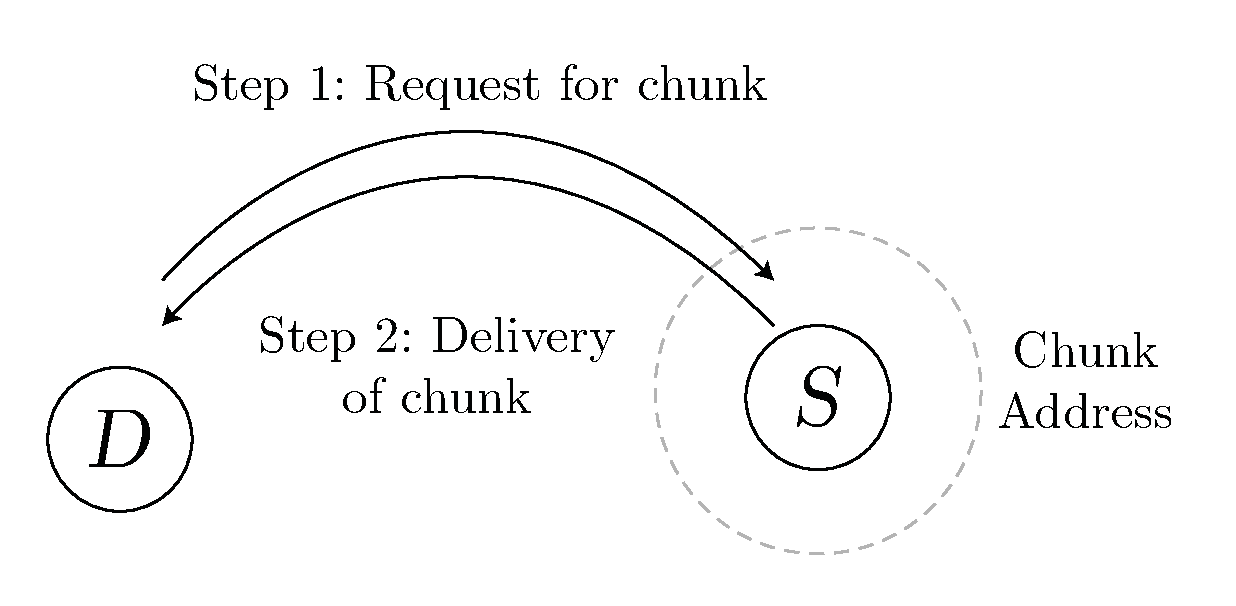
\includegraphics[width=0.7\textwidth]{fig/disc.pdf}
   \caption[Swarm DISC: Distributed Immutable Store for Chunks \statusgreen]{Swarm DISC:  Distributed Immutable Store for Chunks. In step $1$, downloader node $D$ uses forwarding Kademlia routing to request the chunk from a storer node $S$ in the neighbourhood of the chunk address. In step $2$ the chunk is delivered along the same route using forwarding step just backwards.   }
   \label{fig:disc}
\end{figure}

\subsubsection{Constraints}
The \gloss{DISC} storage model is opinionated about which nodes store what content and this implies the following restrictions: 

\begin{enumerate}
    \item \emph{fixed-size chunks} -- Load balancing of content is required among nodes and is realised by splitting content into equal sized units called  \glossplural{chunk} (see \ref{sec:chunks}).
    \item \emph{syncing} -- There must be a process whereby chunks get to where they are supposed to be stored no matter which node uploads them (see \ref{sec:push-syncing}).
    \item \emph{plausible deniability} -- Since nodes do not have a say in what they store, measures should be employed which serve as the basis of legal protection for node operators to plausibly deny knowing (or even being able to know) anything about the chunks' contents (see \ref{sec:chunk-encryption}).
    \item \emph{garbage collection} -- Since nodes commit to store anything close to them, there needs to be a strategy to select which chunks are kept and which are discarded in the presence of storage space constraints (see  \ref{spec:strategy:garbage-collection}). 
\end{enumerate}

\subsubsection{Chunks}\label{sec:chunks}

\glossupperplural{chunk} are the basic storage units used in Swarm's network layer. They are an association of an address with content. Since retrieval in Swarm (\ref{sec:retrieval}) assumes that chunks are stored with nodes close to their address,  the addresses of chunks should also be uniformly distributed in the address space and have their content limited and roughly uniform in size to achieve fair and equal \gloss{load balancing}.  

When chunks are retrieved, the downloader must be able to verify the correctness of the content given the address. Such integrity translates to guaranteeing uniqueness of content associated with an address. In order to protect against frivolous network traffic, third party \glossplural{forwarding node} should be able to verify the integrity of chunks using only local information available to the node.

The deterministic and collision free nature of addressing implies that chunks are unique as a key--value association: If there exists a chunk with an address, then no other valid chunk can have the same address; this assumption is crucial as it makes the chunk store \gloss{immutable}, i.e.\ there is no replace/update operation on chunks. Immutability is beneficial in the context of relaying chunks as nodes can negotiate information about the possession of chunks simply by checking their addresses. This plays an important role in the stream protocol (see \ref{sec:pull-syncing}) and justifies the DISC resolution as \emph{distributed immutable store for chunks}.

To sum up, chunk addressing needs to fulfill the following requirements:

\begin{enumerate}
    \item \emph{deterministic} -- To enable local validation.
    \item \emph{collision free} -- To provide integrity guarantee.
    \item \emph{uniformly distributed} -- To deliver load balancing.
\end{enumerate}

In the current version of Swarm, we support two types of chunk: \glossplural{content addressed chunk} and \glossplural{single owner chunk}. 

\subsection{Content addressed  chunks\statusgreen}\label{sec:content-addressed-chunks}

A \gloss{content addressed chunk} is not assumed to be a meaningful storage unit, i.e. they can be just blobs of arbitrary data resulting from splitting a larger data blob, a file. The methods by which files are disassembled into chunks when uploading and then reassembled from chunks when downloading are detailed in \ref{sec:datastructures}. The data size of a content addressed Swarm chunk is limited to 4 kilobytes. One of the desirable consequences of using this small chunk size is that concurrent retrieval is available even for relatively small files, reducing the latency of downloads. 

\begin{figure}[htbp]
   \centering
   \includegraphics[width=\textwidth]{fig/content-addressed-chunk-3.pdf}
   \caption[Content addressed chunk\statusgreen]{Content addressed chunk. An at most 4KB payload with a 64-bit little endian encoded span prepended to it constitutes the chunk content. The BMT hash of the payload concatenated with the span then yields the content address.}
   \label{fig:content-addressed-chunk}
\end{figure}

\subsubsection{Binary Merkle tree hash}

The canonical content addressed chunk in Swarm is called a \gloss{binary Merkle tree chunk} (\gloss{BMT chunk}).
The address of BMT chunks is calculated using the \gloss{binary Merkle tree hash} algorithm (\gloss{BMT hash}) described in \ref{spec:format:bmt}. The base hash used in \gloss{BMT} is Keccak256, properties of which such as uniformity, irreversibility and collision resistance all carry over to the \gloss{BMT hash} algorithm. As a result of uniformity, a random set of chunked content will generate addresses evenly spread in the address space, i.e.\ imposing storage requirements balanced among nodes.


\begin{figure}[htbp]
   \centering
   \resizebox{1\textwidth}{!}{
   \tikzset{
level/.style={
  sibling distance={(width("$H^126$")+4pt)},
  level distance=15mm,
  line width=.5pt,
},
mtnode/.style={
  minimum width={width("$H^126$")+2pt},
  minimum height={.7cm},
  inner sep=2pt,
  outer sep=2pt,
  rectangle,
  rounded corners=1pt,
  draw,
  line width=.7pt
},
% edge from parent/.style={draw=none},
mtedge/.style={grow=down,draw=none,<-, edge from parent/.style={draw}},
link/.style={draw=none, edge from parent/.style={draw=none}},
mtedgeadj/.style={mtedge, shorten >=10pt  },
mpedge/.style={mtedge, line width=.7pt,densely dashed},
ellip/.style={draw,loosely dotted, shorten >=5mm, thick,<-, edge from parent/.style={draw}},
bubble/.style={minimum height={1cm}, draw=none, align=center},
data/.style={mtnode,fill=gray!50,line width=.7pt},
mppath/.style={mtnode,line width=.7pt},
mpext/.style={mtnode,line width=.7pt},
mpdata/.style={data,line width=.7pt},
mpdataext/.style={data,line width=.7pt}
}

\begin{tikzpicture}
                  % level 7
\node[mtnode](bmtroot){$H_R$}
  child[<-,grow=left,level distance=3cm] { node[bubble] (ash) {BMT Chunk Hash}  }
  child[grow=down]{ node[mtnode] at (-2,0)(root) {$1337$}
    child[<-,grow=left,level distance=3cm] { node[bubble] (ash) {8 byte span}  }
  }
  child[grow=down]{ node[mtnode] at (2,0) (root) {$H^7_0$}
                  % level 6
  child[<-,grow=right,level distance=3cm] { node[bubble] (ash) {BMT Root}  }
  child { node[mppath] (6-0) {$H^6_0$}   % 0
                  % level 5
    child { node[mppath] (5-0) {$H^5_0$}          % 0
      % child[mpedge]
                  % level 4
                  % mppath goes the other way
      child { node[mpext] (4-0) {$H^4_0$}
        % % child[mtedgeadj]
                  % level 3
        child { node[mtnode] (3-0) {$H^3_0$}
              % level 2
          child { node[mtnode] (2-0) {$H^2_0$}
                % level 1
            child { node[mtnode] (1-0) {$H^1_0$}
                % level 0
              child { node[mtnode] (0-0) {$D^0_0$}
                % data level
                child[mtedge] { node[text width=3cm, align=center] (c-0) {32 byte segments.} }
              }
              % % child[mtedgeadj]
              child { node[mtnode] (0-1) {$D^0_1$}
              }
                % level 0
            }
                % level 1
            % child[mtedgeadj]
            child { node[mtnode] {$H^1_{1}$} child[ellip] }
          }
                % level 2
          % child[mtedgeadj]
          child { node[mtnode] {$H^2_{1}$} child[ellip] }
        }
                % level 3
        % child[mtedgeadj]
        child { node[mtnode] {$H^3_{1}$} child[ellip] }
      }
                % level 4
      child[missing]
      child[missing]
      child { node[mppath] (4-1) {$H^4_1$}                 % 1
                % level 3
        child { node[mpext] (3-4) {$H^3_4$} child[ellip] }
        % child[mpedge]
        child { node[mppath] (3-5) {$H^3_5$}  % 1
                % level 2
          % child[mpedge]
          child { node[mppath] (2-10) {$H^2_{10}$}           % 0
                % level 1
            child { node[mpext] (1-21) {$H^1_{21}$} child[ellip] }
            % child[mpedge]
            child { node[mppath] (1-22) {$H^1_{22}$}         % 1
                % level 0
              child { node[mppath] (0-42) {$D^0_{42}$}       % 0
              }
                % level 0
              % child[mpedge]
              child { node[mpext] (0-43) {$D^0_{43}$}
              }
                % level 0
            }
                % level 1
          }
                % level 2
          % child[mpedge]
          child { node[mpext] (2-11) {$H^2_{11}$} child[ellip] }
        }
                % level 3
        % child[missing]
      }
                % level 4
    }
                % level 5
    child[missing]
    % child[mpedge]
    child[missing]
    child { node[mpext] (5-1) {$H^5_1$} child[ellip] }
  }
                % level 6
  child[missing]
  child[missing]
  % child[mtedgeadj]
  child[missing]
  child  { node[mpext] (6-1) {$H^6_1$}
                % level 5
    child { node[mtnode] (5-2) {$H^5_2$} child[ellip] }
    child[missing]
    % child[mtedgeadj]
    child { node[mtnode] (5-3) {$H^5_3$}
                % level 4
      child { node[mtnode] {$H^4_{6}$} child[ellip] }
      % child[mtedgeadj]
      child { node[mtnode] (4-7) {$H^4_7$}
                % level 3
        child { node[mtnode] {$H^3_{14}$} child[ellip] }
        % child[mtedgeadj]
        child { node[mtnode] (3-15) {$H^3_{15}$}
                % level 2
          child { node[mtnode] {$H^3_{30}$} child[ellip] }
          % child[mtedgeadj]
          child { node[mtnode] (2-31) {$H^2_{31}$}
                % level 1
            child { node[mtnode] {$H^1_{62}$} child[ellip] }
            % child[mtedgeadj] {node {}}
            child { node[mtnode] (1-63) {$H^1_{63}$}
                % level 0
              child { node[mtnode] (0-126) {$D^0_{126}$}
              }
              % child[mtedgeadj]
              child { node[mtnode] (0-127) {$D^0_{127}$}
                child { node[draw=none, text width=6cm, align=center] (spanann) {zero padding if needed to fill 4Kb.} }
              }
                % 0
            }
                % 1
          }
                % 2
        }
                % 3
      }
                % 4
    }
               % 5
  }
}               % 6
 ;
\end{tikzpicture}}
   \caption[BMT: Binary Merkle Tree hash used as chunk hash in Swarm \statusgreen]{BMT (Binary Merkle Tree) chunk hash in Swarm: the 1337 bytes of chunk data is segmented into 32 byte segments. Zero padding is used to fill up the rest up to 4 kilobytes. Pairs of segments are hashed together using Keccak256 to build up the binary tree. On level 8, the binary Merkle root is prepended with the 8 byte span and hashed to yield the BMT chunk hash.`}
   \label{fig:BMT}
\end{figure}

The BMT chunk address is the hash of the 8 byte span and the root hash of a \gloss{binary Merkle tree} (\gloss{BMT}) built on the 32-byte segments of the underlying data (see figure \ref{fig:BMT}). If the chunk content is less than 4k, the hash is calculated as if the chunk was padded with all zeros up to 4096 bytes.

This structure allows for compact \gloss{inclusion proofs} with a 32-byte resolution. An inclusion proof is a proof that one string is a substring of another string, for instance, that a string is included in a chunk. Inclusion proofs are defined on a data segment of a particular index, see figure \ref{fig:chunk-inclusion}. Such Merkle proofs are also used as proof of custody when storer nodes provide evidence that they possess a chunk (see \ref{sec:postage-lottery}). Together with the Swarm file hash (see \ref{sec:files} and \ref{spec:format:files}), it allows for logarithmic inclusion proofs for files, i.e.\ proof that a string is found to be part of a file.


\begin{figure}[htbp]
\centering
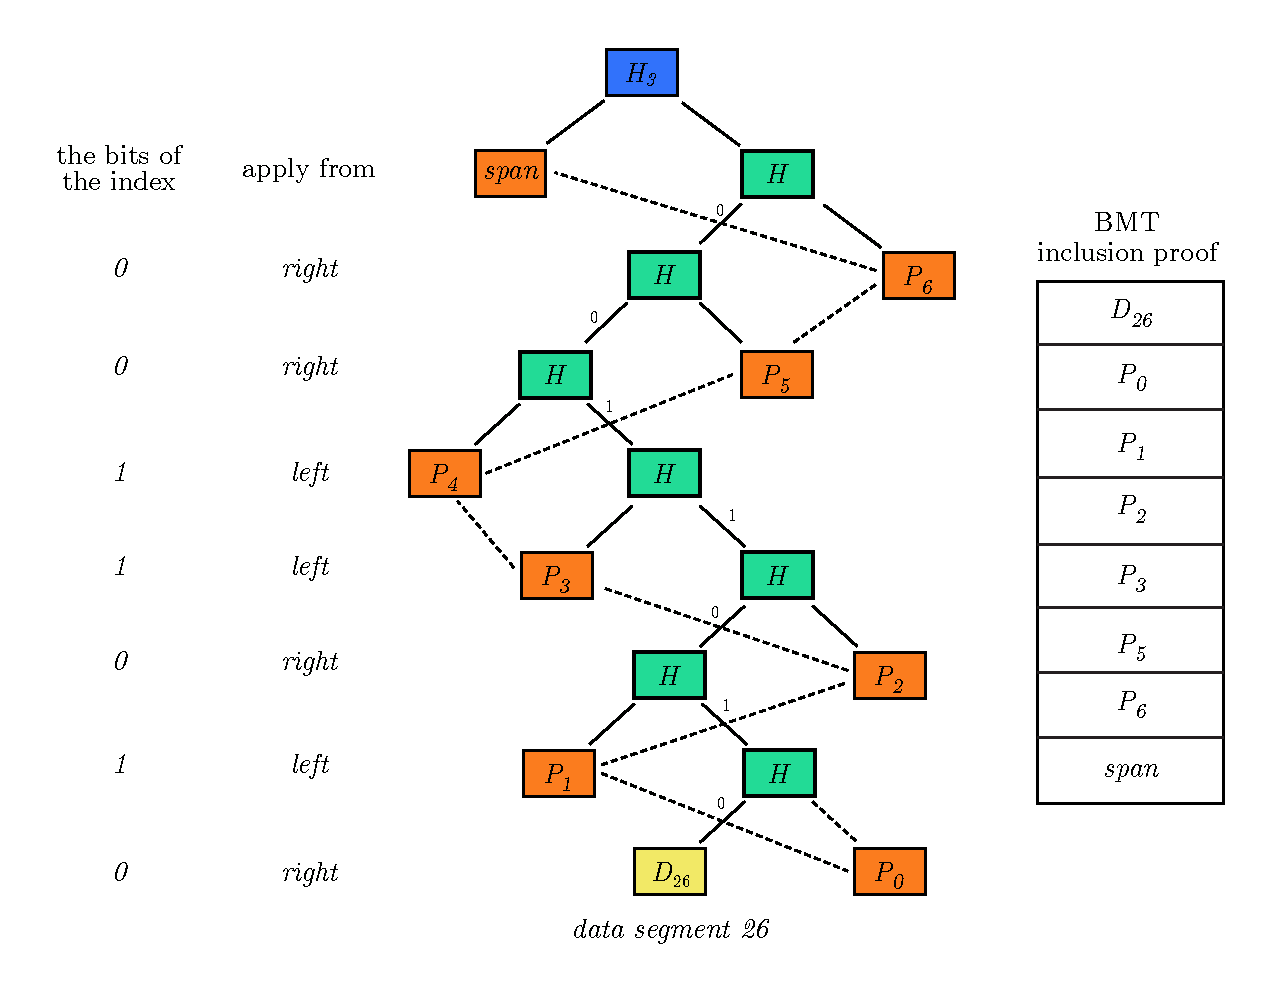
\includegraphics[width=\textwidth]{fig/inclusion-proof.pdf}
\caption[Compact segment inclusion proofs for chunks \statusgreen]{Compact segment inclusion proofs for chunks. Assume we need proof for segment 26 of a chunk (yellow). The orange hashes of the BMT are the sister nodes on the path from the data segment up to the root and constitute what needs to be part of a proof. When these are provided together with the root hash and the segment index, the proof can be verified. The side on which proof item $i$ needs to be applied depends on the $i$-th bit (starting from least significant) of the binary representation of the index. Finally the span is prepended and the resulting hash should match the chunk root hash.}
\label{fig:chunk-inclusion}
\end{figure}


\subsection{Single-owner chunks\statusgreen}\label{sec:single-owner-chunks}

With \glossplural{single owner chunk}, a user can assign arbitrary data to an address and attest chunk integrity with their digital signature. The address is calculated as the hash of an \gloss{identifier} and an \gloss{owner}. The chunk content is presented in a  structure composed of the identifier, the \gloss{payload} and a signature attesting to the association of identifier and payload (see figure \ref{fig:single-owner-chunks}).

\begin{itemize}
    \item \emph{content}: 
\begin{itemize}
    \item \emph{identifier} -- 32 bytes arbitrary identifier, 
    \item \emph{signature} -- 65 bytes $\langle r,s,v \rangle$ representation of an EC signature (32+32+1 bytes),
    \item \emph{span} -- 8 byte little endian binary of uint64 chunk span,
    \item \emph{payload} -- max 4096 bytes of regular chunk data.
\end{itemize}
    \item \emph{address} -- Keccak256 hash of identifier + owner account.
\end{itemize}

\begin{figure}[htbp]
   \centering
   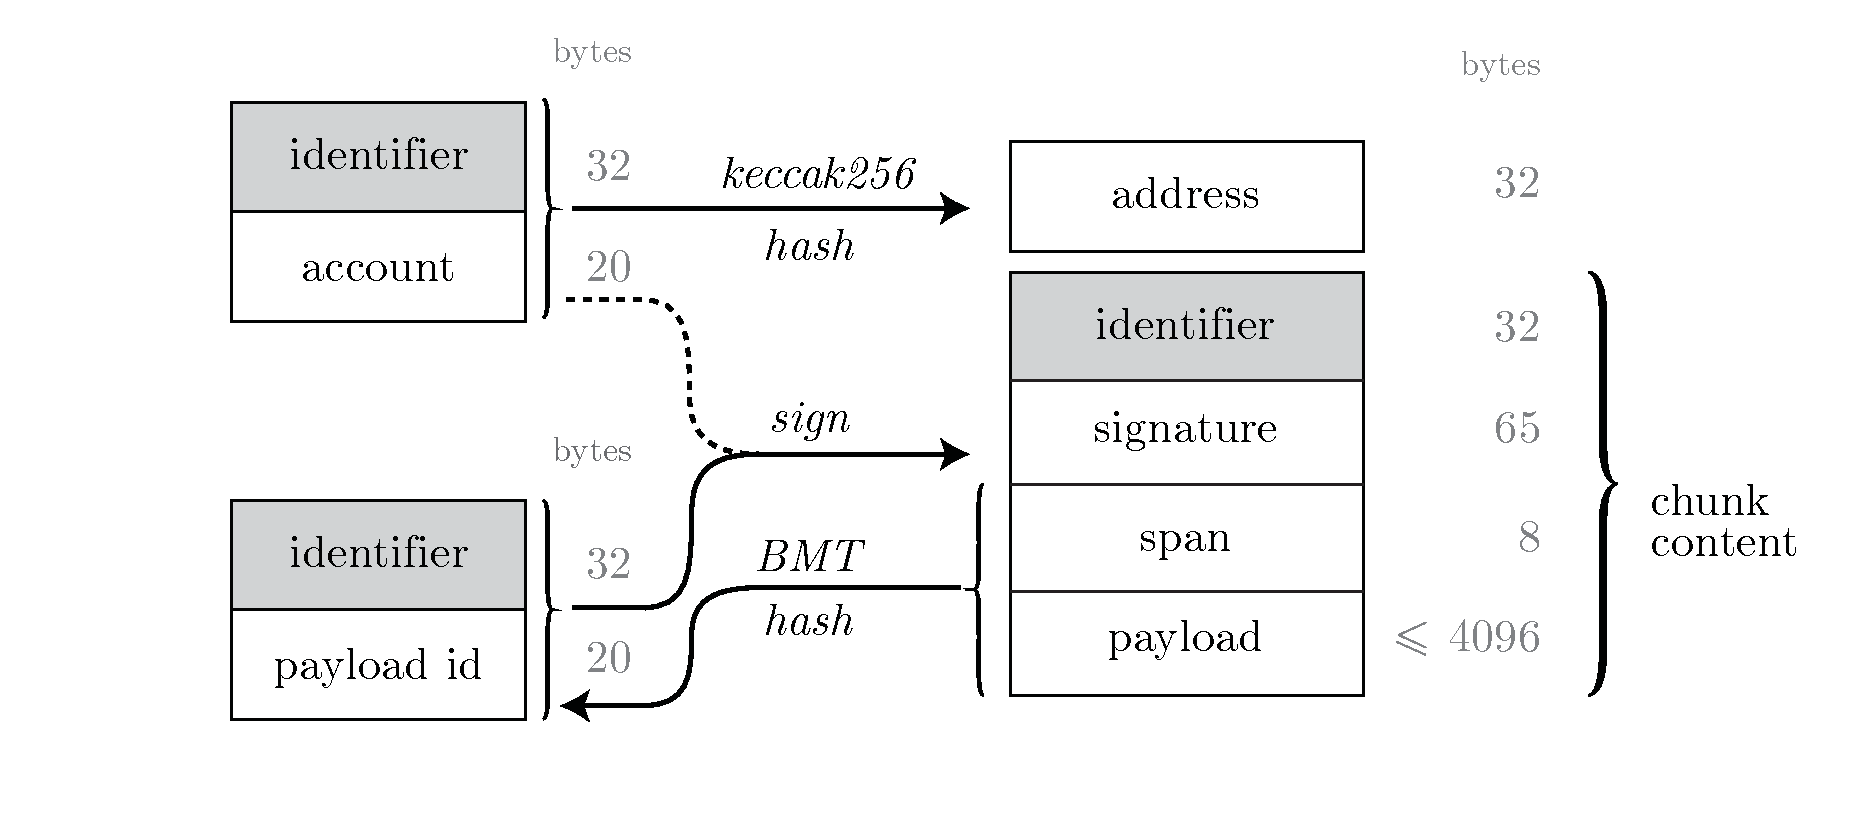
\includegraphics[width=\textwidth]{fig/single-owner-chunk.pdf}
   \caption[Single-owner chunk\statusgreen]{Single-owner chunk. The chunk content is composed of headers followed by an at most 4KB payload. The last header field is the 8 byte span prepended just like in content addressed chunks. The first two header fields provide single owner attestation of integrity: an identifier and a signature signing off on the identifier and the BMT hash of span and payload. The address is the hash of the id and the signer account.}
   \label{fig:single-owner-chunks}
\end{figure}

Validity of a \gloss{single owner chunk} is checked with the following process:

\begin{enumerate}
    \item Deserialise the chunk content into fields for identifier, signature and payload.
    \item Construct the expected plain text composed of the identifier and the \gloss{BMT hash} of the payload.
    \item Recover the owner's address from the signature using the plain text.
    \item Check the hash of the identifier and the owner (expected address) against the chunk address.
\end{enumerate}

Single-owner chunks offer a virtual partitioning of part of the address space into subspaces associated with the single owner. Checking their validity is actually an authentication verifying that the owner has write access to the address with the correct identifier.

As suggested by the span and the length of the payload, a single owner chunk can encapsulate a regular content addressed chunk. Anyone can simply reassign a regular chunk to an address in their subspace designated by the identifier (see also \ref{sec:notification-requests}).


It should be noted that the notion of integrity is somewhat weaker for single owner chunks than in the case of content addressed chunks: After all, it is, in principle, possible to assign and sign any payload to an identifier. Nonetheless, given the fact that the chunk can only be created by a single owner (of the private key that the signature requires), it is reasonable to expect uniqueness guarantees because we hope the node will want to comply with application protocols to get the desired result. However, if the owner of the private key signs two different payloads with the same identifier and uploads both chunks to Swarm, the behaviour of the network is unpredictable. Measures can be taken to mitigate this in layer (3) and are discussed later in detail in \ref{sec:feed-integrity}.

With two types of chunk, integrity is linked to collision free hash digests, derived from either a single owner and an arbitrary identifier attested by a signature or directly from the content. This justifies the resolution of the DISC acronym as \emph{data integrity through signing or content address}.

\subsection{Chunk encryption\statusgreen}\label{sec:chunk-encryption}

Chunks should be encrypted by default. Beyond client needs for confidentiality, encryption has two further important roles. (1) Obfuscation of chunk content by encryption provides a degree of \gloss{plausible deniability}; using it across the board makes this defense stronger. (2) The ability to choose arbitrary encryption keys together with the property of uniform distribution offer predictable ways of \gloss{mining chunks}, i.e.\ generating an encrypted variant of the same content so that the resulting chunk address satisfies certain constraints, e.g. is closer to or farther away from a particular address. This is an important property used in (1) price arbitrage (see \ref{sec:pricing}) and (2) efficient use of postage stamps (see \ref{sec:postage-stamps}).


\begin{figure}[htbp]
    \centering
    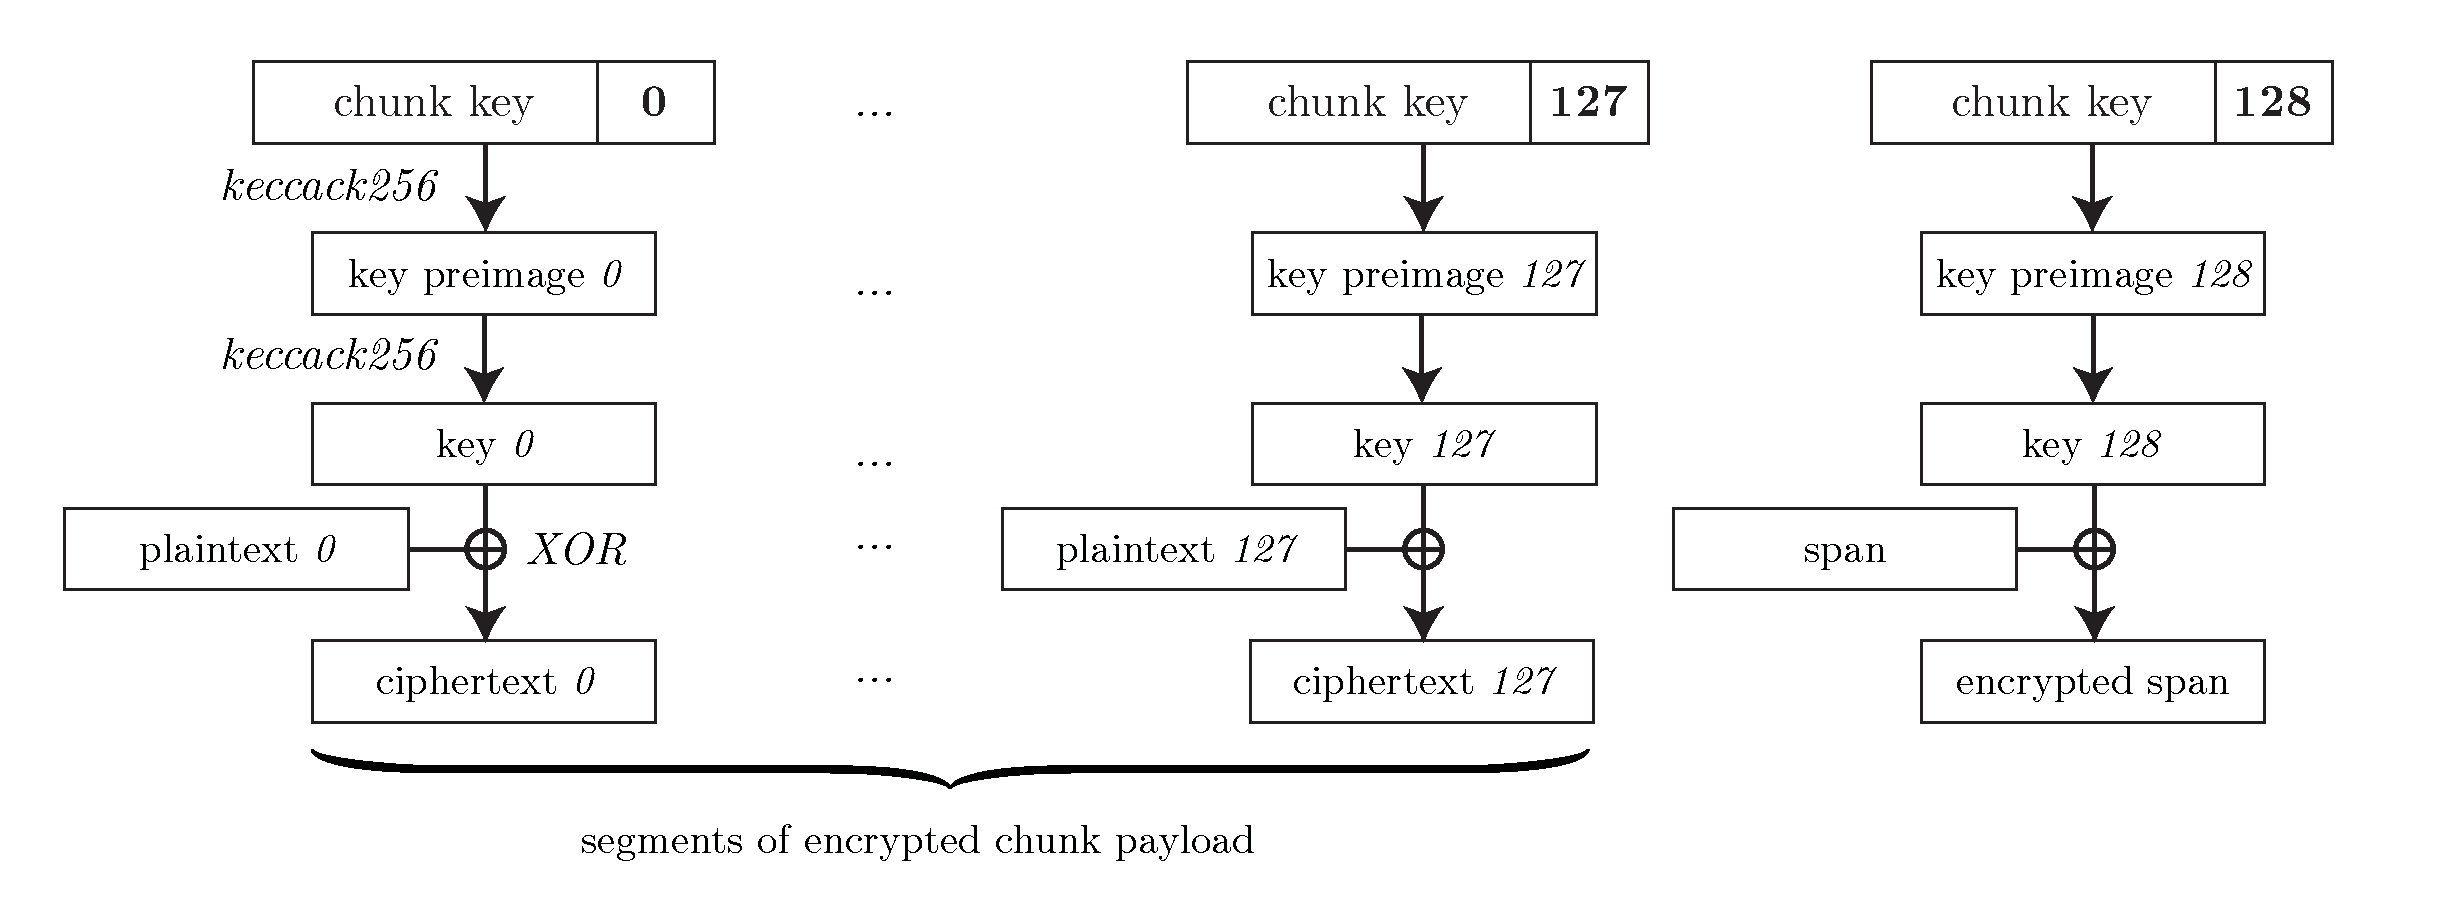
\includegraphics[width=\textwidth]{fig/chunk-encryption.pdf}
    \caption[Chunk encryption in Swarm \statusgreen]{Chunk encryption in Swarm. Symmetric encryption with a modified counter-mode block cipher. The plaintext input is the content padded with random bytes to 4 kilobytes. The span bytes are also encrypted as if they were continuations of the payload.}
    \label{fig:chunk-encryption}
\end{figure}


Chunk encryption (see figure \ref{fig:chunk-encryption}) is formally specified in \ref{spec:format:encryption}. Chunks shorter than 4 kilobytes are padded with random bytes (generated from the chunk encryption seed). The full chunk plaintext is encrypted and decrypted using a stream cipher; XOR with a PRNG seeded with the corresponding symmetric key. In order not to increase the attack surface by introducing additional cryptographic primitives, the stream cipher of choice is using Keccak256 in counter mode, i.e. hashing together the key with a counter for each consecutive segment of 32 bytes. In order to allow selective disclosure of individual segments being part of an encrypted file, yet leak no information about the rest of the file, we add an additional step of hashing to derive the encryption key for a segment in the chunk. This scheme is easy and cheap to implement in the \gloss{EVM}, lending itself to use in smart contracts constraining the plaintext of encrypted Swarm content. 

The prepended metadata encoding the chunk span is also encrypted as if it was a continuation of the chunk, i.e. with counter 128. Encrypted chunk content is hashed using the \gloss{BMT hash} digest just as unencrypted ones are. The fact that a chunk is encrypted may be guessed from the \gloss{span value}, but apart from this, in the network layer, encrypted chunks behave in exactly the same way as unencrypted ones.

\glossupperplural{single owner chunk} can also be encrypted, which simply means that they wrap an encrypted regular chunk. Therefore, their payload and span reflect the chunk content encryption described above, the hash signed with the identifier is the \gloss{BMT hash} of the encrypted span and payload, i.e. the same as that of the wrapped chunk.

\subsection{Redundancy by replication\statusgreen}\label{sec:redundancy-by-local-replication}

It is important to have a resilient means of requesting data. To achieve this Swarm implements the approach of defence in depth. In the case that a request fails due to a problem with forwarding, one can retry with another peer or, to guard against these occurrences, a node can start concurrent \glossplural{retrieve request} right away. However, such fallback options are not available if all the single last node that stores the chunk drop out from the network. Therefore, redundancy is of major importance to ensure data availability. If the closest node is the only storer of the requested data and it drops out of the network, then there is no way to retrieve the content. This basic scenario is handled by ensuring each set of \gloss{nearest neighbours} hold replicas of each chunk that is closest to any one of them, duplicating the storage of chunks and therefore providing data redundancy. 

\subsubsection{Size of nearest neighbourhoods}

If the Kademlia connectivity is defined over storer nodes, then in a network with Kademlia topology there exists a depth $d$ such that (1) each \gloss{proximity order bin} less than $d$ contains at least $k$ storer peers, and (2) all \glossplural{storer node} with \gloss{proximity order} $d$ or higher are actually connected peers. In order to ensure data redundancy, we can add to this definition a criterion that (3) the nearest neighbourhood defined by $d$ must contain at least $r$ peers.

Let us define \gloss{neighbourhood size} $\mathit{NHS}_x(d)$  as the cardinality of the neighbourhood defined by depth $d$ of node $x$. 
Then, a node has Kademlia connectivity with redundancy factor $r$ if there exists a depth $d$ such that (1) each proximity order bin less than $d$ contains at least $k$ storer peers ($k$ is the bin density parameter see \ref{sec:bindensity}), and (2) all storer nodes with proximity order $d$ or higher are actually connected peers, and (3) $\mathit{NHS}_x(d)\geq r$.

We can then take the highest depth $d'$ such that (1) and (2) are satisfied. Such a $d$ is guaranteed to exist and the \glossupper{hive protocol} is always able to bootstrap it. As we decrease $d'$, the amount of different neighbourhood grow proportionally, so for any redundancy parameter not greater than the network size $r\leq N=\mathit{NHS}_x(0)$, there will be a highest $0<d_r\leq d'$ such that $\mathit{NHS}_x(d_r)\geq r$. Therefore, \gloss{redundant Kademlia connectivity} is always achievable. 



For a particular redundancy, the area of the fully connected neighbourhood defines an \gloss{area of responsibility}. The proximity order boundary of the area of responsibility defines a \gloss{radius of responsibility} for the node. A storer node is said to be \emph{responsible} for (storing) a chunk if the chunk address falls within the node's radius of responsibility.

It is already instructive at this point to show neighbourhoods and how they are structured, see figure \ref{fig:nearest-neighbours}. 

\begin{figure}[htbp]
   \centering
   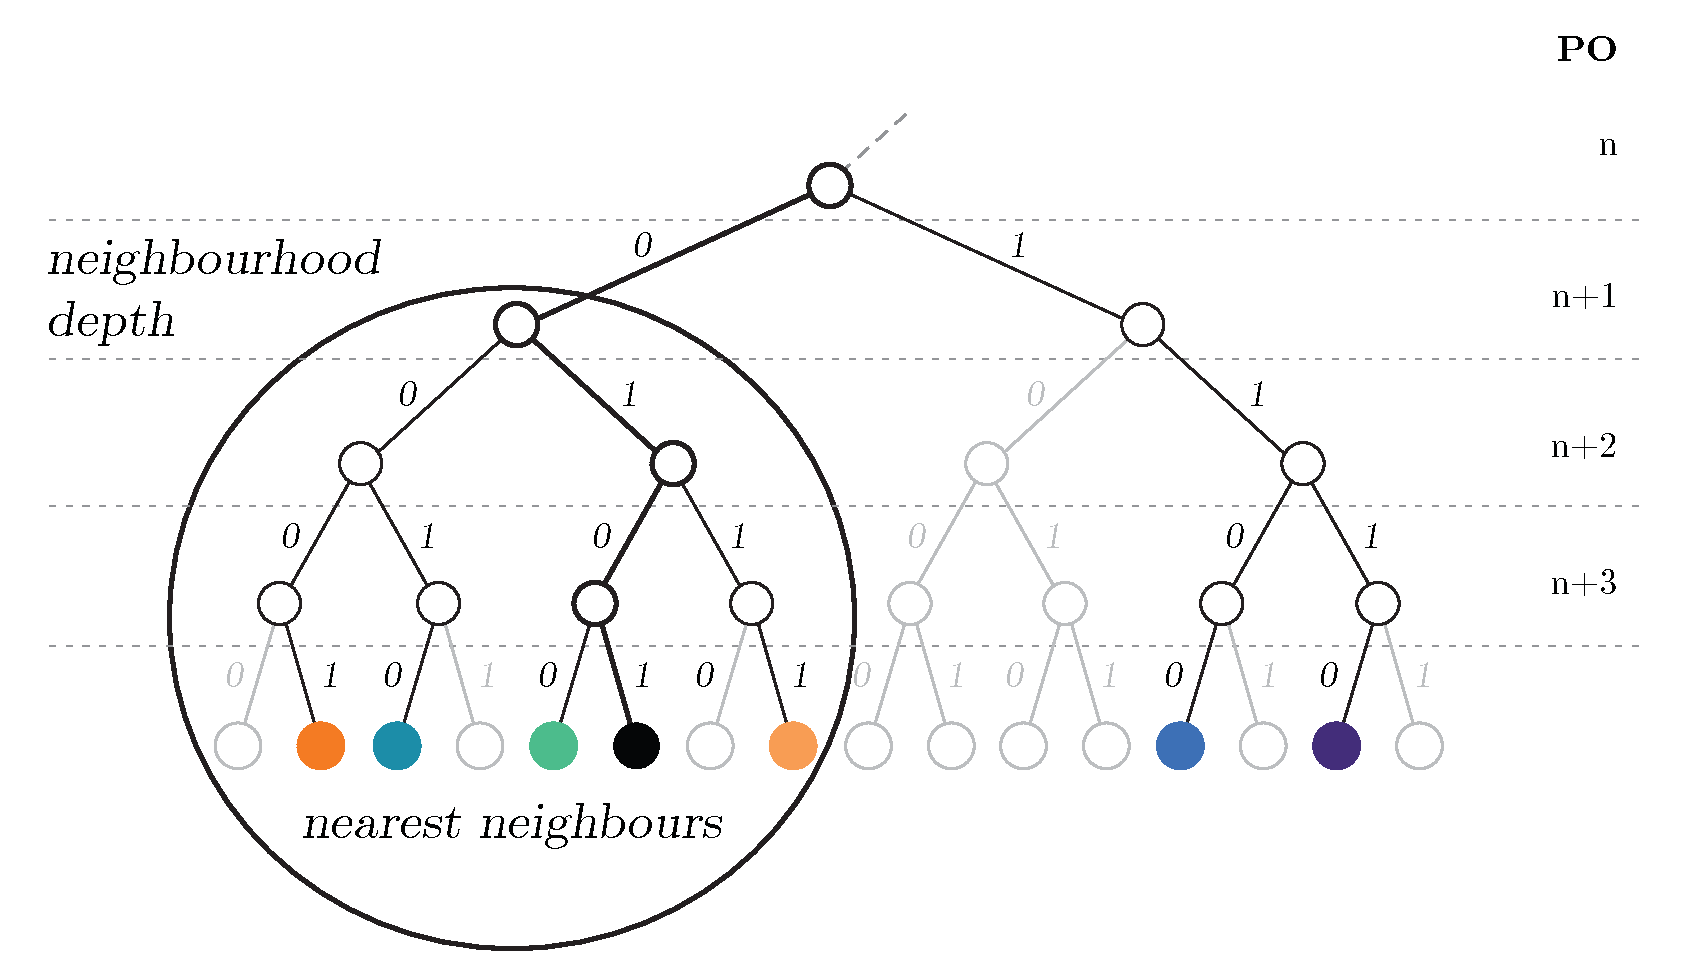
\includegraphics[width=\textwidth]{fig/nearest-neighbours-2.pdf}\\
   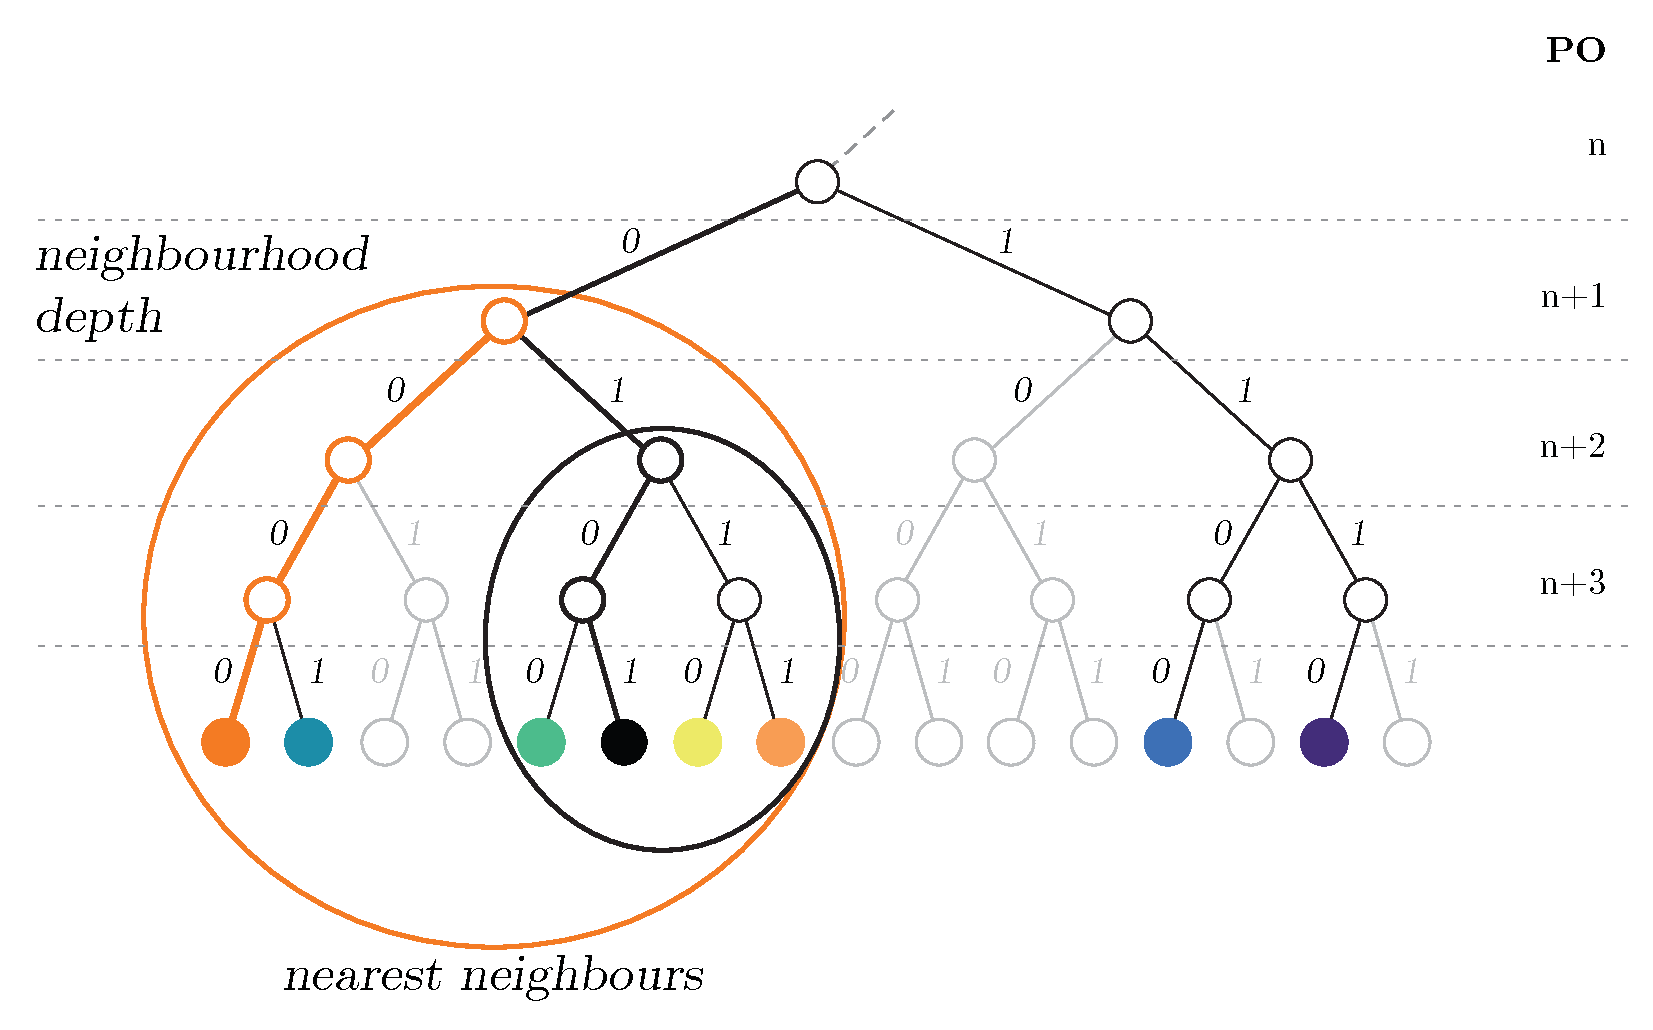
\includegraphics[width=\textwidth]{fig/asymmetric-nodes2.pdf}
   \caption[Nearest neighbours \statusgreen]{Nearest neighbours. \textbf{Top}: Each PO defines a neighbourhood, the neighbourhood depth of the node (black circle) is defined as the highest PO such that the neighbourhood has at least R=4 peers (redundancy parameter) and all shallower bins are non-empty. \textbf{Bottom}: An asymmetric neighbourhood. Nearest neighbours of the orange node include the black node but not the other way round.}
   \label{fig:nearest-neighbours}
\end{figure}


\subsubsection{Redundant retrievability}

A chunk is said to have \gloss{redundant retrievability} with degree $r$ if it is retrievable and would remain so even after any $r$ nodes responsible for it leave the network. The naive approach presented so far requiring the single closest node to keep the content can be interpreted as degree zero retrievability. If nodes in their area of responsibility fully replicate their content (see \ref{sec:pull-syncing}), then every chunk in the Swarm DISC is redundantly retrievable with degree $r$. Let us take the node $x$ that is closest to a chunk $c$. Since it has Kademlia connectivity with redundancy $r$, there are $r+1$ nodes responsible for the chunk in a neighbourhood fully connected and replicating content. After $r$ responsible nodes drop out, there is just one node remaining which still has the chunk. However, if Kademlia connectivity is maintained as the $r$ nodes leave, this node will continue to be accessible by any other node in the network and therefore the chunk is still retrievable. Now, for the network to ensure all chunks will remain redundantly retrievable with degree $r$, the nodes comprising the new neighbourhood formed due to the reorganising of the network must respond by re-syncing their content to satisfy the protocol's replication criteria. This is called the guarantee of \gloss{eventual consistency}.

\subsubsection{Resource constraints}

Let us assume then that (1) the forwarding strategy that relays requests along \glossplural{stable node} and (2) the storage strategy that each node in the nearest neighbourhood (of $r$ storer nodes) stores all chunks the address of which fall within their radius of responsibility. As long as these assumptions hold, each chunk is retrievable even if $r$ storer nodes drop offline simultaneously. As for (2), we still need to assume that every node in the nearest neighbour set can store each chunk. Realistically, however, all nodes have resource limitations. With time, the overall amount of distinct chunks ever uploaded to Swarm will increase indefinitely. Unless the total storage capacity steadily increases, we should expect that the nodes in Swarm are able to store only a subset of chunks. Some nodes will reach the limit of their storage capacity and therefore face the decision whether to stop accepting new chunks via syncing or to make space by deleting some of their existing chunks. 

The process that purges chunks from their local storage is called \gloss{garbage collection}. The process that dictates which chunks are chosen for garbage collection is called the \gloss{garbage collection strategy} (see  \ref{spec:strategy:garbage-collection}). For a profit-maximizing node, it holds that it is always best to garbage-collect the chunks that are predicted to be the least profitable in the future and, in order to maximize profit, it is desired for a node to get this prediction right (see \ref{sec:postage-stamps}). So, in order to factor in these capacity constraints, we will introduce the notion of \gloss{chunk value} and modify our definitions using the minimum value constraint:

In Swarm's DISC, at all times there is a chunk value $v$ such that every chunk with a value greater than $v$ is both retrievable and eventually (after syncing) redundantly retrievable with degree $r$. 

This value ideally corresponds to the relative importance of preserving the chunk that uploaders need to indicate. In order for storer nodes to respect it, the value should also align with the profitability of chunk and is therefore expressed in the pricing of uploads (see \ref{sec:capacity-pressure}).

% \subsection{}\label{sec:}

\section{Push and pull: chunk retrieval and syncing\statusgreen}\label{sec:push-and-pull}
\green{}
In this section, we demonstrate how chunks actually move around in the network: How they are pushed to the storer nodes in the neighbourhood they belong to when they are uploaded, as well as how they are pulled from the storer nodes when they are downloaded.

\subsection{Retrieval\statusgreen}\label{sec:retrieval}

In a distributed chunk store, we say that a chunk is an \gloss{accessible chunk} if a message is routable between the requester and the node that is closest to the chunk. Sending a retrieve request message to the chunk address will reach this node.  Because of \gloss{eventual consistency}, the node closest to the chunk address will store the chunk. Therefore, in a \gloss{DISC} distributed chunk store with healthy Kademlia topology all chunks are always accessible for every node.

\subsubsection{Chunk delivery}

For retrieval, accessibility needs to be complemented with a process to have the content delivered back to the requesting node, preferably using only the chunk address. There are at least three alternative ways to achieve this (see figure \ref{fig:chunk-delivery}):

\begin{enumerate}
    \item \gloss{direct delivery} -- The chunk delivery is sent via a direct underlay connection. 
    \item \gloss{routed delivery} -- The chunk delivery is sent as message using routing.
    \item \gloss{backwarding} -- The chunk delivery response simply follows the route along which the request was forwarded, just backwards all the way to the originator.
\end{enumerate}


\begin{figure}[htbp]
   \centering
   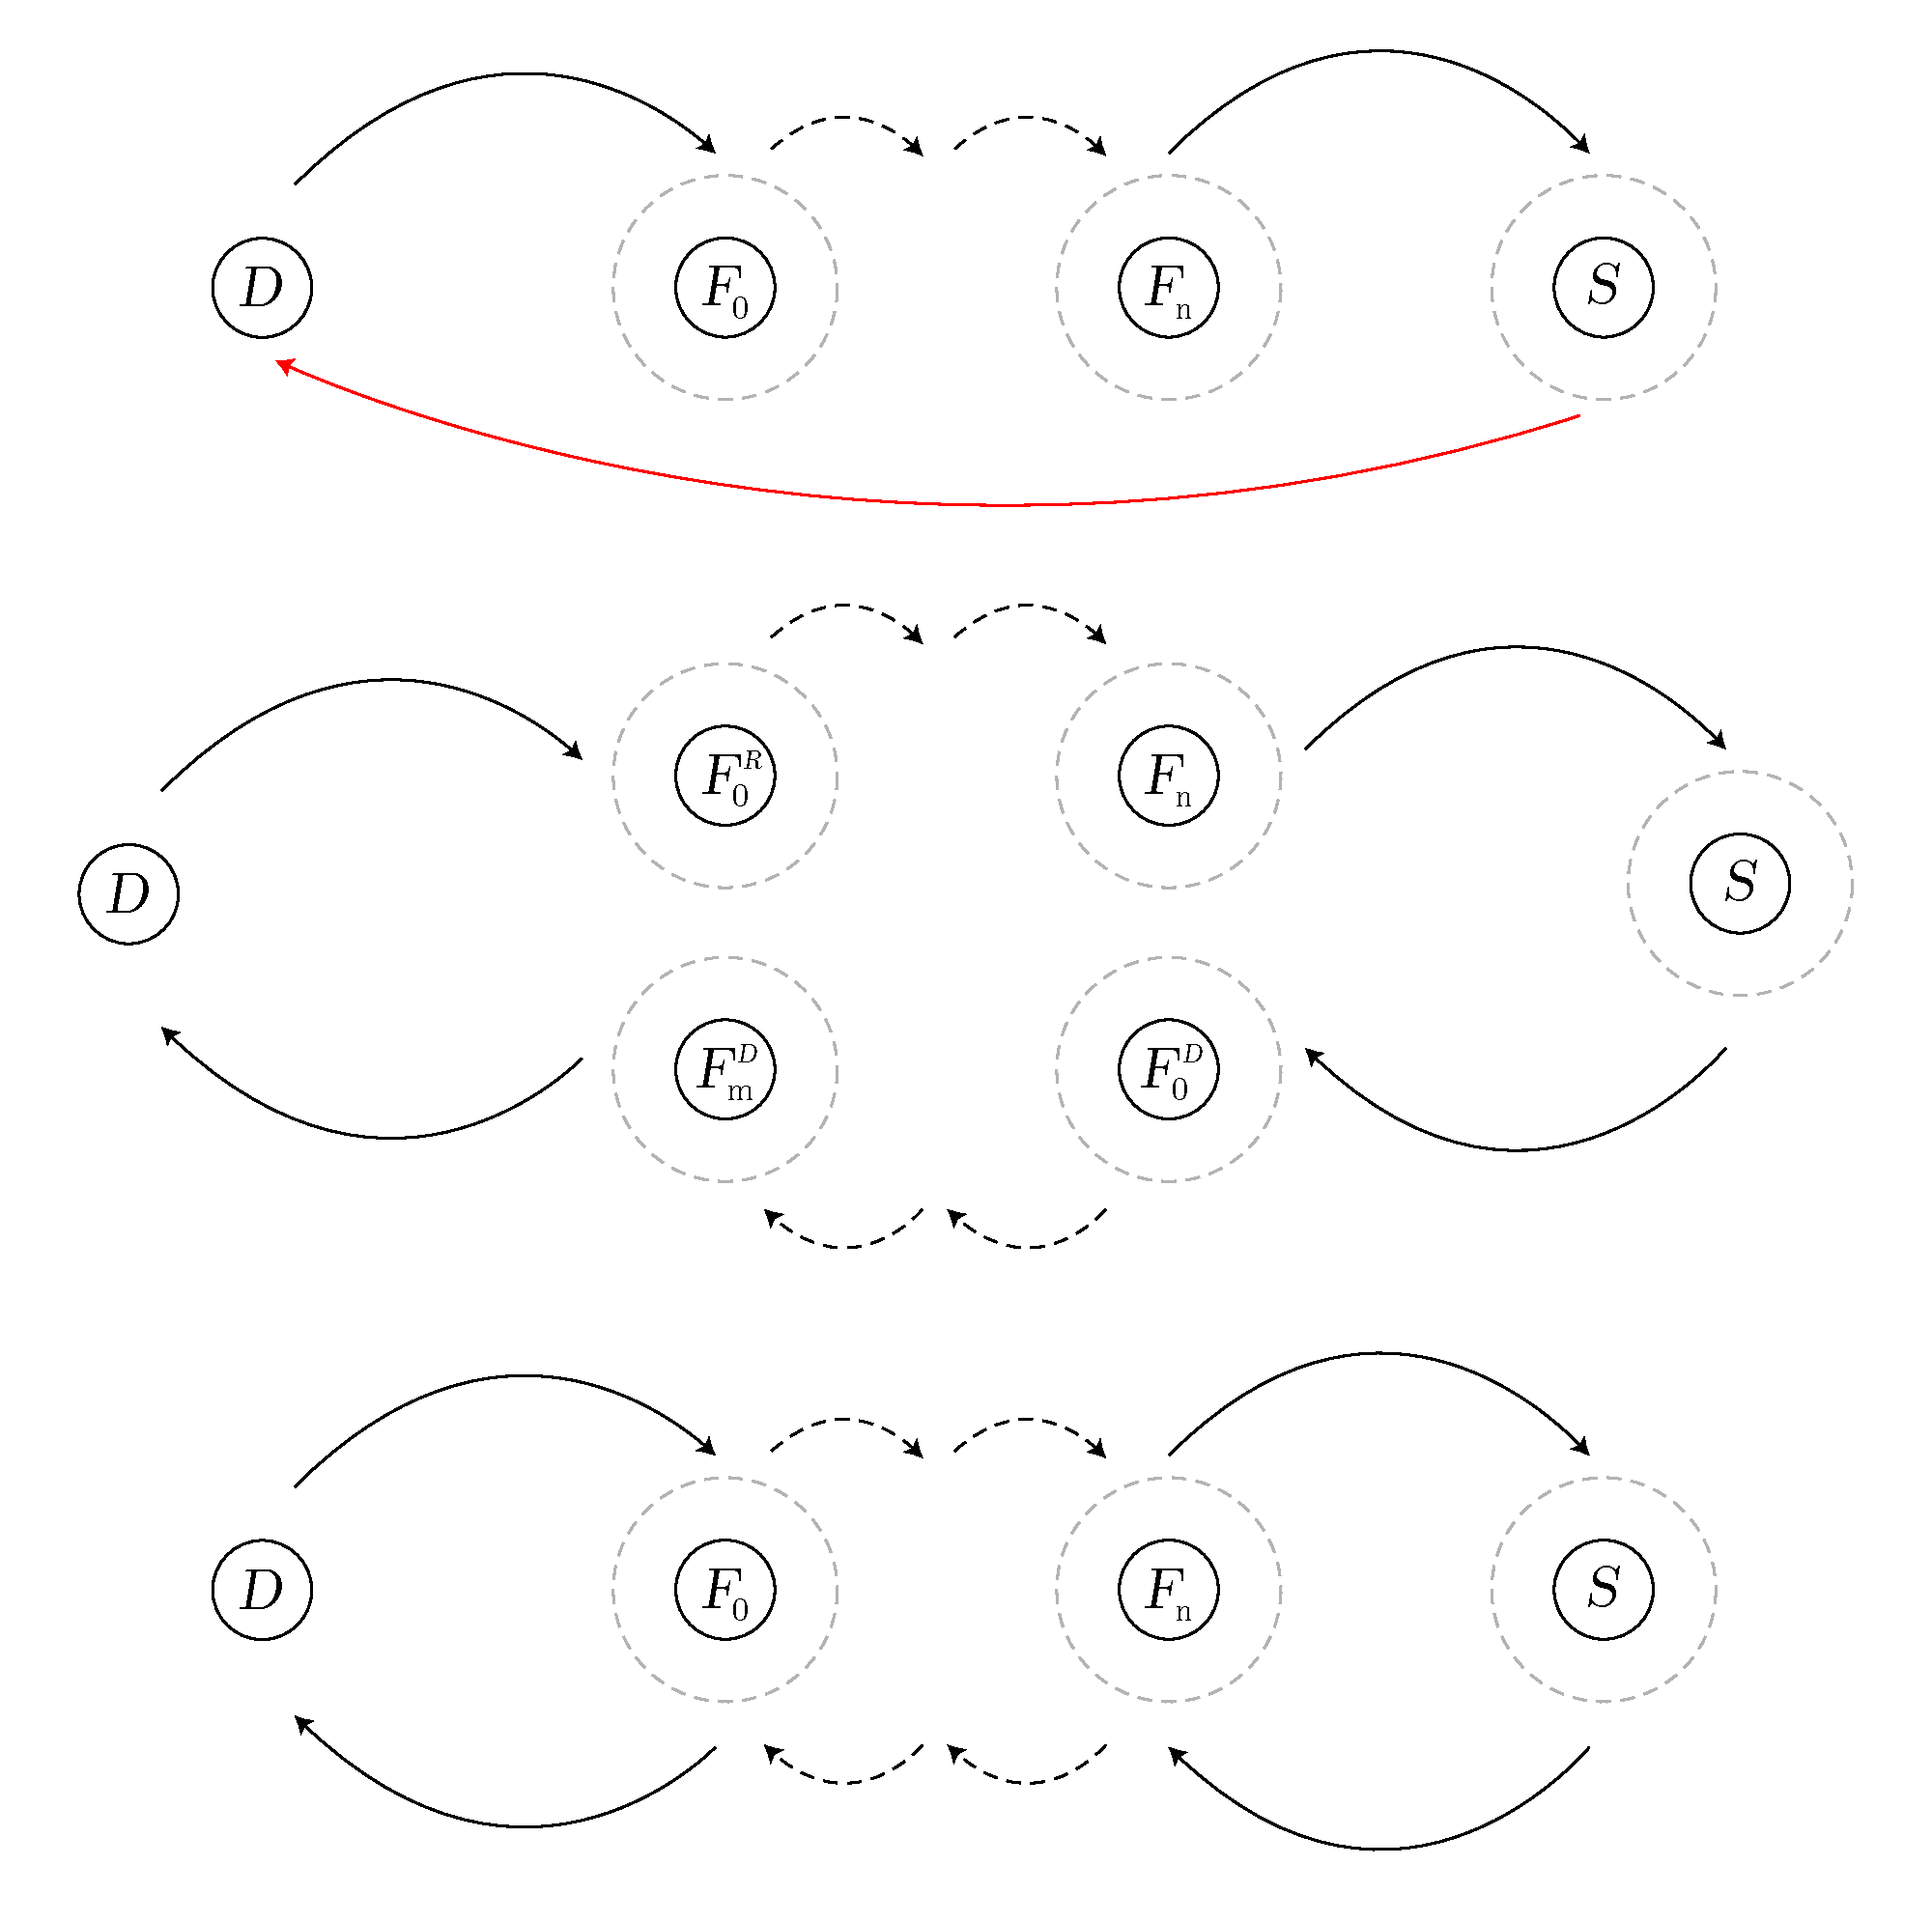
\includegraphics[width=\textwidth]{fig/chunk-delivery.pdf}
   \caption[Alternative ways to deliver chunks: direct, routed and backward \statusgreen]{Alternative ways to deliver chunks. \textbf{Top:} \emph{direct delivery}: via direct underlay connection. \textbf{Centre:} \emph{routed delivery}: chunk is sent using Kademlia routing. \textbf{Bottom:} \gloss{backwarding} re-uses the exact peers on the path of the request route to relay the delivery response.}
   \label{fig:chunk-delivery}
\end{figure}

Firstly, using the obvious direct delivery, the chunk is delivered in one step via a lower level network protocol. This requires an ad-hoc connection with the associated improvement in latency traded off for worsened security of privacy.%
%
\footnote{Beeline delivery has some merit, i.e. bandwidth saving and better latency, so we do not completely rule out the possibility of implementing it. 
}
Secondly, using routed delivery, a chunk is delivered back to its requestor using ad-hoc routing as determined from the storer's perspective at the time of sending it. Whether direct or routed, allowing deliveries routed independently of the request route presupposes that the requestor's address is (at least partially) known by the storer and routing nodes and as a consequence, these methods leak information identifying the requestor. However, with forwarding--backwarding Kademlia this is not necessary: The storer node responds back to their requesting peer with the delivery while intermediate \glossplural{forwarding node} remember which of their peers requested what chunk. When the chunk is delivered, they pass it on back to their immediate requestor, and so on until it eventually arrives at the node that originally requested it. In other words, the chunk delivery response simply follows the request route back to the originator (see figure \ref{fig:request-response}).  Since it is the reverse of the forwarding, we can playfully call this \gloss{backwarding}. Swarm uses this option, which makes it possible to disclose no requestor identification in any form, and thus Swarm implements completely \gloss{anonymous retrieval}. 

\begin{figure}[htbp]
   \centering
   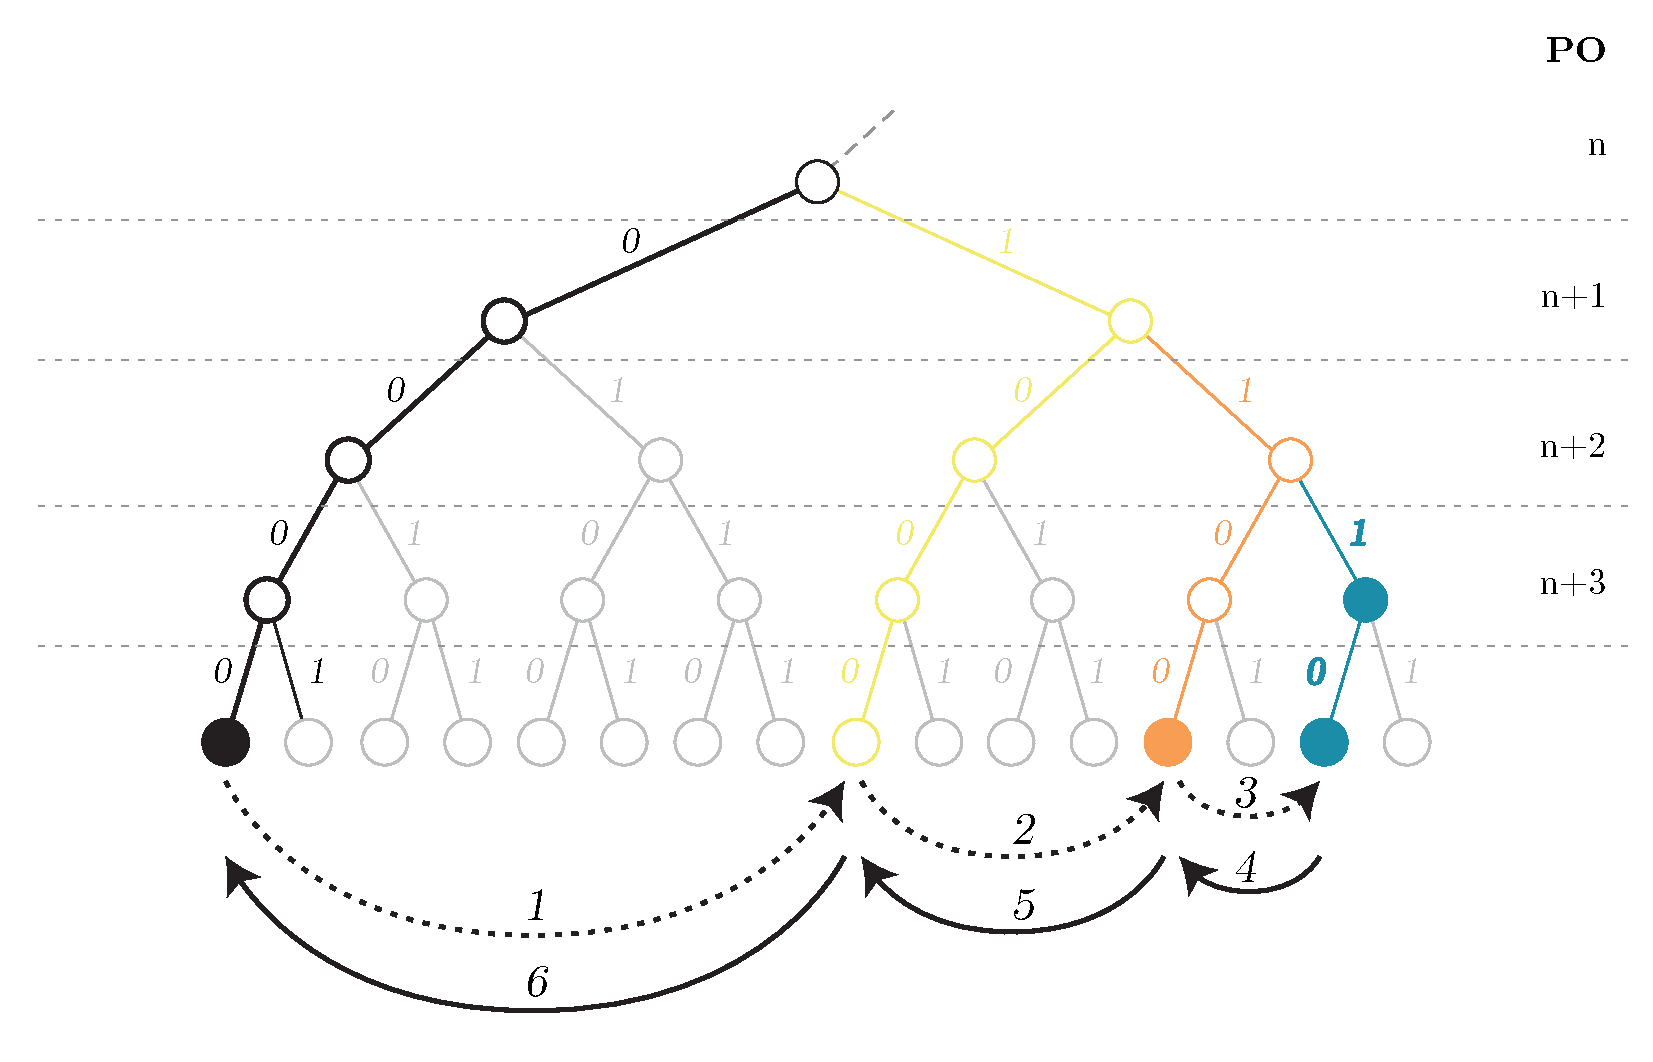
\includegraphics[width=\textwidth]{fig/request-response-forwarding.pdf}
   \caption[Backwarding: a pattern for anonymous request-response round-trips in forwarding Kademlia \statusgreen]{Backwarding: pattern for anonymous request--response round-trips in forwarding Kademlia. Here a node with overlay address $...0000...$ sending a request to target $....1111...$ to which the closest online node is $...1110...$ The leading ellipsis represents the prefix shared by the requestor and target and has a length of $n$ bits, the trailing ellipsis represents part of the address that is not relevant for routing as at that depth nodes are already unique. The request uses the usual Kademlia forwarding, but the relaying nodes on the way remember the peer a request came from so that when the response arrives, they can \emph{backward} it (i.e.\ pass it back) along the same route.}
   \label{fig:request-response}
\end{figure}

Requestor anonymity by default in the retrieval protocol is a crucial feature that Swarm insists upon to ensure user privacy and censorship-resistant access.

\begin{figure}[htbp]
   \centering
   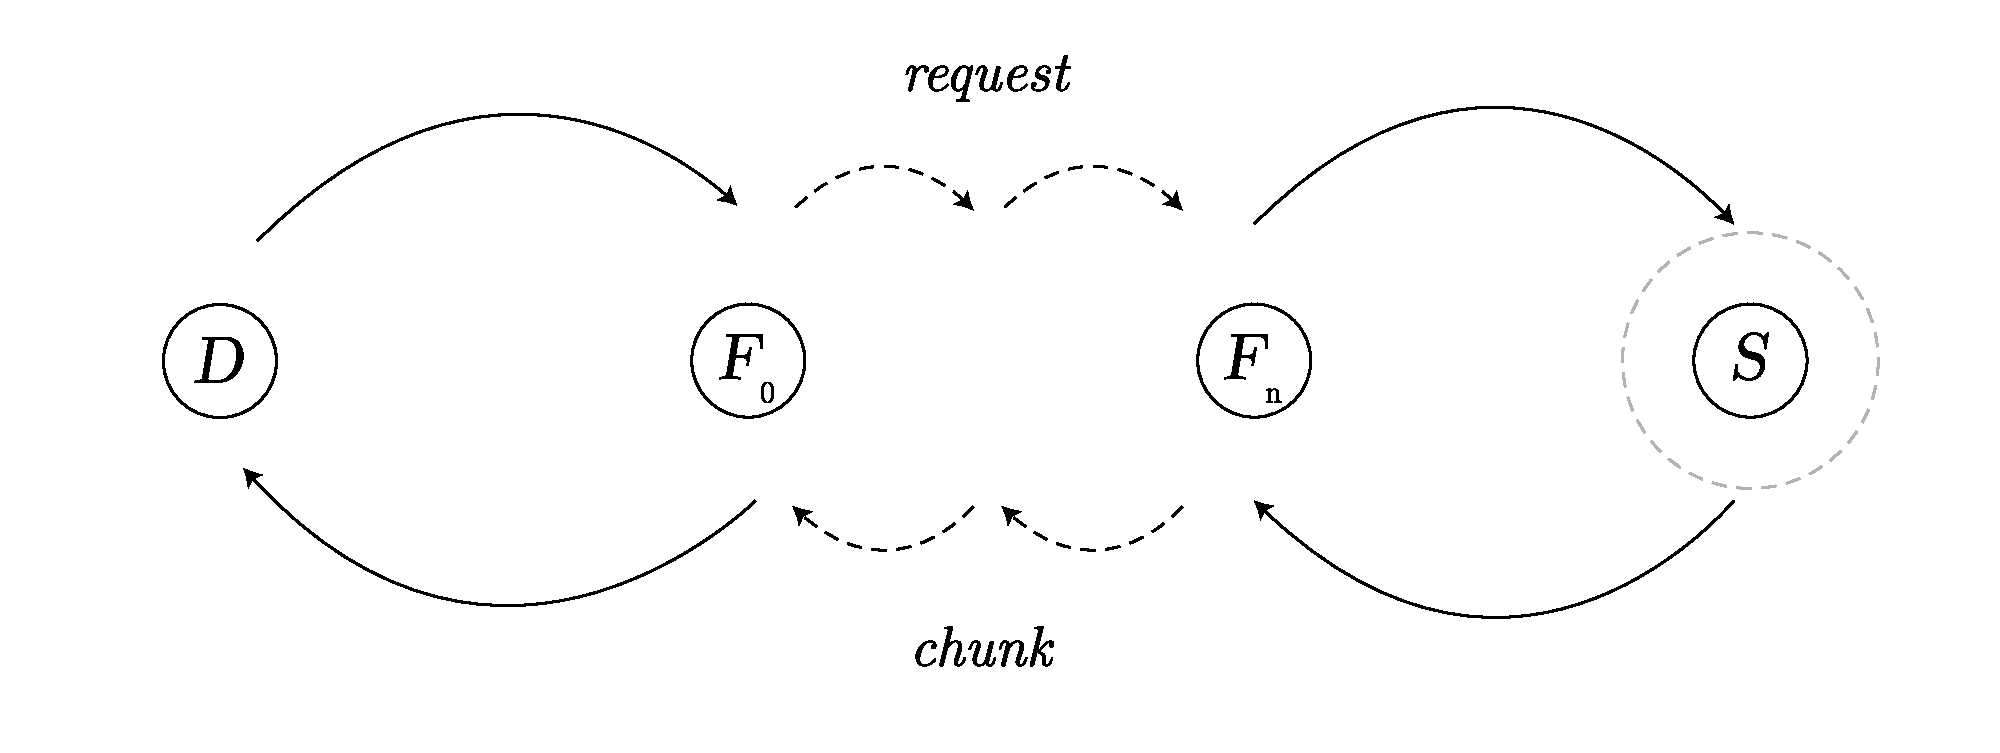
\includegraphics[width=\textwidth]{fig/retrieval.pdf}
   \caption[Retrieval \statusgreen]{Retrieval. Node $D$ (Downloader) sends a retrieve request to the chunk's address. Retrieval uses forwarding Kademlia, so the request is relayed via forwarding nodes $F_0$, ..., $F_n$ all the way to node $S$, the storer node closest to the chunk address. The chunk is then delivered by being passed back along the same route to the downloader.}
   \label{fig:retrieval}
\end{figure}

The generic solution of implementing retrieval by backwarding as depicted in figure \ref{fig:retrieval} has further benefits relating to spam protection, scaling and incentivisation, which are now discussed in the remainder of this section.

\subsubsection{Protection against unsolicited chunks}

In order to remember requests, the \gloss{forwarding node} needs to create a resource for which it bears some cost (it takes up space in memory). The requests that are not followed by a corresponding delivery should eventually be garbage collected, so there needs to be a defined time period during which they are active. Downstream peers also need to be informed about the timeout of this request. This makes sense since the originator of the request will want to attach a time to live duration to the request to indicate how long it will wait for a response.  

Sending unsolicited chunks is an offence as it can lead to \gloss{denial of service (DoS)}. By remembering a request, nodes are able to recognise unsolicited chunk deliveries and penalise the peers sending them. Chunks that are delivered after the request expires will be treated as unsolicited. Since there may be some discrepancy assessing the expiry time between nodes, there needs to be some tolerance for unsolicited chunk deliveries, but if they go above a particular (but still small) percentage of requests forwarded, the offending peer is disconnected and blacklisted. Such local sanctions are the easiest and simplest way to incentivise adherence to the protocol (see \ref{sec:sanctions}). 

\subsubsection{Rerequesting}

There is the potential for a large proportion of Swarm nodes to not be always stably online. Such a high churn situation would be problematic if we used the naive strategy of forwarding requests to any one closer node: If a node on the path were to go offline before delivery is completed, then the request-response round trip is broken, effectively rendering the chunk requested not retrievable. Commitment to pay for a chunk is considered void if the connection to the requested peer is dropped, so there is no harm in re-requesting the chunk from another node (see \ref{spec:strategy:forwarding}).


\subsubsection{Timeout vs not found}

Note that in Swarm there is no explicit negative response for chunks not being found. In principle, the node that is closest to the retrieved address can tell that there is no chunk at this address and could issue a "not found" response, however this is not desirable for the following reason. While the closest node to a chunk can verify that a chunk is indeed not at the place in the network where it is supposed to be, all nodes further away from the chunk cannot credibly conclude this as they cannot verify it first-hand and all positive evidence about the chunk's retrievability obtained later is retrospectively plausibly deniable. 

All in all, as long as delivery has the potential to create earnings for the storer, the best strategy is to keep a pending request open until it times out and be prepared in case the chunk should appear. There are several ways the chunk could arrive after the request: (1) syncing from existing peers (2) appearance of a new node or (3) if a request precedes upload, e.g. the requestor has already "subscribed" to a single owner address (see \ref{sec:messaging}) to decrease latency of retrieval. This is conceptually different from the usual server-client based architectures where it makes sense to expect a resource to be either on the host server or not. 
 

\subsubsection{Opportunistic caching}

Using the backwarding for chunk delivery responses to retrieve requests also enables \gloss{opportunistic caching}, where a \gloss{forwarding node} receives a chunk and the chunk is then saved in case it will be requested again. This mechanism is crucial in ensuring that Swarm scales the storage and distribution of popular content automatically (see \ref{sec:caching}).

\subsubsection{Incentives}

So far, we have shown that by using the retrieval protocol and maintaining Kademlia connectivity, nodes in the network are capable of retrieving chunks. However, since forwarding is expending a scarce resource (bandwidth), without providing the ability to account for this bandwidth use, network reliability will be contingent on the proportion of freeriding and altruism. To address this, in section \ref{sec:incentivisation}, we will outline a system of economic incentives that align with the desired behaviour of nodes in the network. When these profit maximising strategies are employed by node operators, they give rise to emergent behaviour that is beneficial for users of the network as a whole.
 
\subsection{Push syncing\statusgreen}\label{sec:push-syncing}
 
In the previous sections, we presented how a network of nodes maintaining a Kademlia overlay topology can be used as a distributed chunk store and how Forwarding Kademlia routing can be used to define a protocol for retrieving chunks.
When discussing retrieval, we assumed that chunks are located with the node whose address is closest to theirs. This section describes the protocol responsible for realising this assumption: ensuring delivery of the chunk to its prescribed storer after it has been uploaded to any arbitrary node.

This network protocol, called \gloss{push syncing}, is analogous to chunk retrieval: First, a chunk is relayed to the node closest to the chunk address via the same route as a retrieval request would be, and then in response a \gloss{statement of custody receipt} is passed back along the same path (see figure \ref{fig:push-syncing}). The statement of custody sent back by the storer to the \gloss{uploader} indicates that the chunk has reached the neighbourhood from which it is then universally retrievable. By tracking these responses for each constituent chunk of an upload, uploaders can make sure that their upload is fully retrievable by any node in the network before sharing or publishing the address of their upload. Keeping this count of chunks push-synced and receipts received serves as the back-end for a \emph{progress bar} that can be displayed to the uploader to give positive feedback of the successful propagation of their data across the network (see \ref{sec:upload} and \ref{spec:api:tags}).


\begin{figure}[htbp]
   \centering
   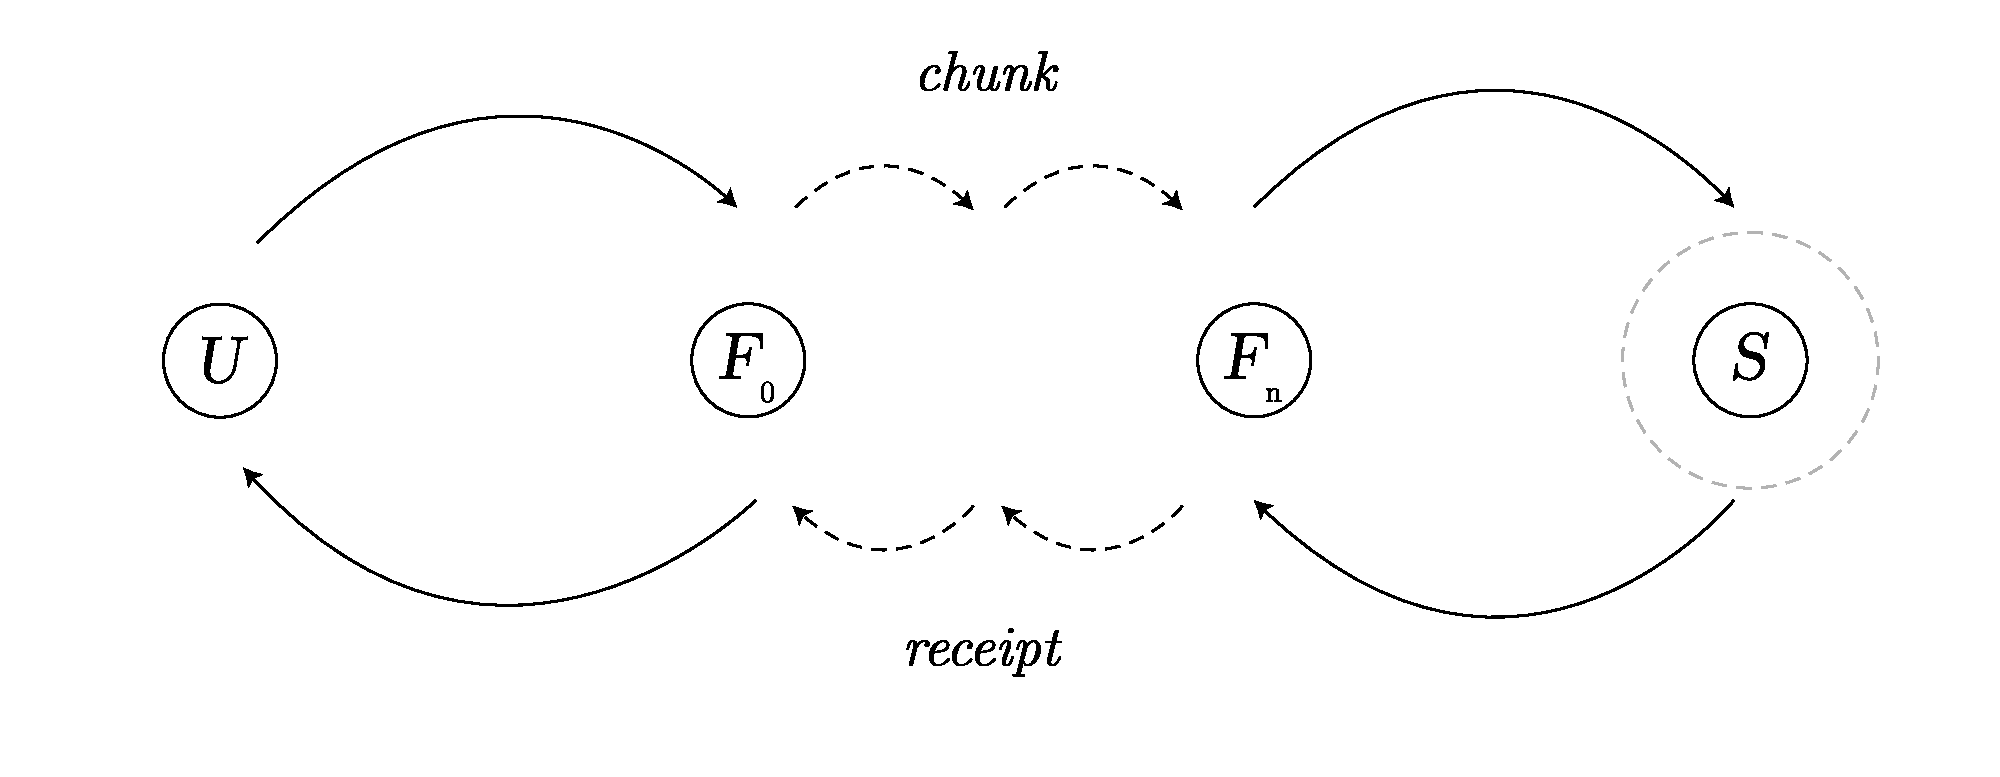
\includegraphics[width=\textwidth]{fig/push-sync.pdf}
   \caption[Push syncing \statusgreen]{Push syncing. Node $U$ (Uploader) push-syncs a chunk to the chunk's address. Push-sync uses forwarding, so the chunk is relayed via forwarding nodes $F_0$, ..., $F_n$ all the way to node $S$, the storer node closest to the chunk address (the arrows represent transfer of the chunk  via direct peer-to-peer connection). A statement of custody receipt signed by $S$ is then passed back along the same route as an acknowledgment to the uploader.}
   \label{fig:push-syncing}
\end{figure}

Statements of custody are signed by the nodes that claim to be the closest to the address. 
Similarly to downloaders in the retrieval protocol, the identity of uploaders can also remain hidden, hence forwarding Kademlia can implement \gloss{anonymous uploads}.

Another similarity is that in order to allow backwarding for responses, nodes should remember which peer sent a particular chunk. This record should persist for a short period while the statement of custody responses are expected. When this period ends, the record is removed. A statement of custody not matching a record is considered unsolicited and is allowed only up to a small percentage of all push-sync traffic with a peer. Going above this tolerance threshold is sanctioned with disconnection and blacklisting (see \ref{sec:sanctions}).

In this section we described how the logistics of chunk uploads can be organised with a network protocol using Forwarding Kademlia routing with response backwarding. However, this solution is not complete until it is secured with aligned incentives: The strategy to follow this protocol should be incentivised and DoS abuse should be disincentivised. These are discussed later in detail in \ref{sec:postage-stamps} and \ref{sec:push-sync-incentives}).

\subsection{Pull syncing\statusgreen}\label{sec:pull-syncing}

\glossupper{pull syncing} is the protocol that is responsible for the following two properties: 

\begin{itemize}
    \item \emph{eventual consistency} -- Syncing neighbourhoods as and when the topology changes due to churn or new nodes joining.
    \item \emph{maximum resource utilisation} -- Nodes can pull chunks from their peers to fill up their surplus storage.%
%
\footnote{Maximum storage utilisation may not be optimal in terms of the profitability of nodes. Put differently, storer nodes have an optimal storage capacity, based on how often content is requested from them. This means that in practice, profit-optimised maximum utilisation of storage capacity requires operators to run multiple node instances.}
\end{itemize}

Pull syncing is node centric as opposed to chunk centric, i.e. it makes sure that a node's storage is filled if needed, as well as syncing chunks within a neighbourhood. When two nodes are connected they will start syncing both ways so that on each peer connection there is bidirectional chunk traffic. The two directions of syncing are managed by distinct and independent \emph{streams} (see \ref{spec:protocol:pull-sync}). In the context of a stream, the consumer of the stream is called \gloss{downstream peer} or client, while the provider is called the \gloss{upstream peer} or server. 

When two nodes connect and engage in \gloss{chunk synchronisation}, the upstream peer offers all the chunks it stores locally in a data stream per proximity order bin. To receive chunks closer to the downstream peer than to the upstream peer, a downstream peer can subscribe to the chunk stream of the proximity order bin that the upstream peer belongs to in their Kademlia table. If the peer connection is within the nearest neighbour depth $d$, the client subscribes to all streams with proximity order bin $d$ or greater. As a result, peers eventually replicate all chunks belonging to their area of responsibility.

A pull syncing server's behaviour is referred to as being that of a \gloss{stream provider} in the stream protocol (see \ref{spec:protocol:pull-sync}). Nodes keep track of when they stored a chunk locally by indexing them with an ever increasing storage count, called the \gloss{bin ID}. For each proximity order bin, upstream peers offer to stream chunks in descending order of storage timestamp. As a result of syncing streams on each peer connection, a chunk can be synced to a downstream peer from multiple upstream peers. In order to save bandwidth by not sending data chunks to peers that already have them, the stream protocol implements a round-trip: Before sending chunks, the upstream peer offers a batch of chunks identified by their address, to which downstream responds with stating which chunks in the offered batch they actually need (see figure \ref{fig:pull-syncing}). Note that downstream peer decides whether they have the chunk based on the chunk address. Thus, this method critically relies on the chunk integrity assumption discussed in \ref{sec:chunks}.


\begin{figure}[htbp]
   \centering
   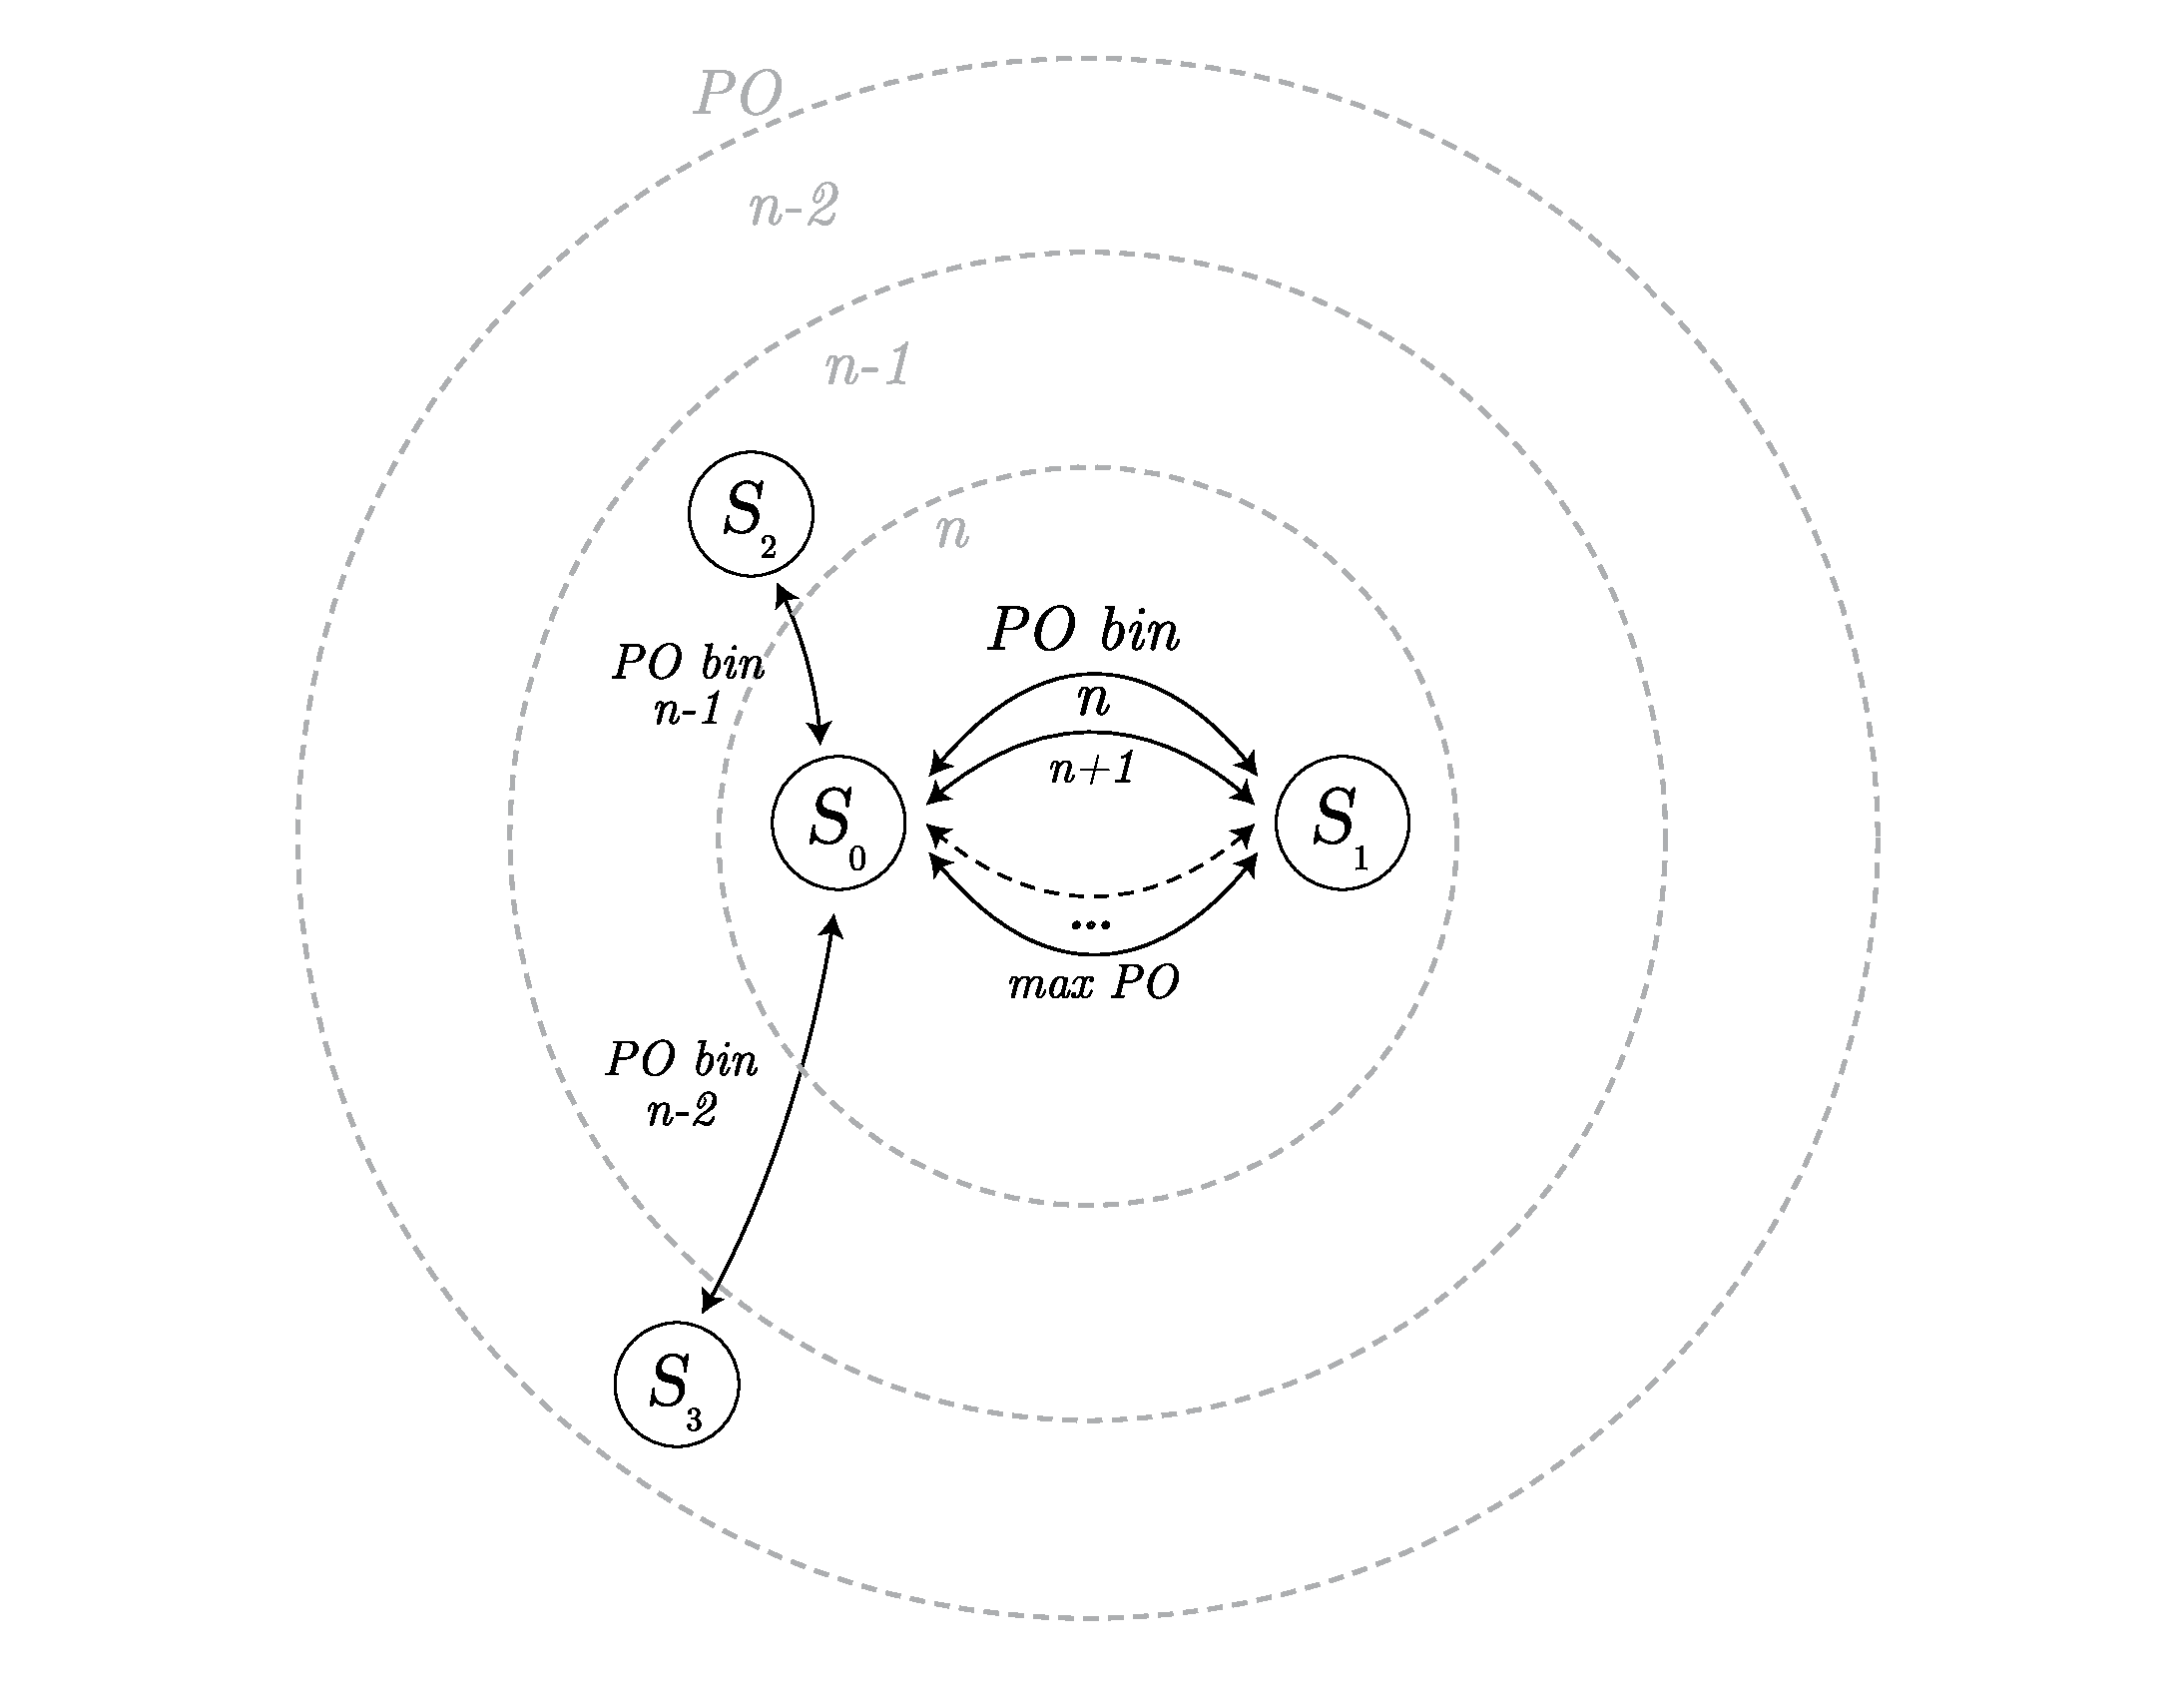
\includegraphics[width=\textwidth]{fig/pull-sync.pdf}
   \caption[Pull syncing \statusgreen]{Pull syncing. Nodes continuously synchronise their nearest neighbourhood. If they have free capacity they also pull sync chunks belonging to shallower bins from peers falling outside the neighbourhood depth.}
   \label{fig:pull-syncing}
\end{figure}

In the context of a peer connection, a client is said to be \emph{synced} if it has synced all the chunks of the upstream peer. Note that due to disk capacity limitations, nodes must impose a value cutoff and as such "all chunks" reads as shorthand for "all chunks having value greater than $v$" ($v$ is a constant ranking function, the origin of which is discussed later in \ref{sec:capacity-pressure}). In order for a node to promise they store all chunks with value greater than $v$, all its neighbours must have stored all chunks greater than value $v$. In other words, nodes syncing inherit the maximum such value from among their storer peers. 

If chunks are synced in the order they are stored, this may not result in the node always having the most profitable (most often requested) chunks. Thus it may be advisable to sync chunks starting with the most popular ones according to upstream peers and finish syncing when storage capacity is reached. In this way, a node's limited storage will be optimised. Syncing and garbage collection are discussed further in \ref{sec:postage-stamps} and \ref{sec:capacity-pressure} and a consolidated client strategy is specified in \ref{spec:strategy:pull-sync}.

To conclude this section, we show how the criteria of \gloss{eventual consistency} are met in a healthy Swarm. Chunks found in the local store of any node will become retrievable after being synced to their storers. This is because as long as those as peers in the network pull chunks closer to them than to the upstream peer, each chunk travels a route that would also qualify as valid a forwarding path in the push-sync protocol. If new nodes are added, and old nodes drop out, neighbourhoods change, but as long as local redundancy is high enough that churn can not render previously retrievable chunks non-retrievable, neighbourhoods eventually replicate their content and redundancy is restored. Consider the unlikely event that a whole new neighbourhood is formed and the nodes that originally held the content belonging to this neighbourhood end up outside of it and therefore those chunks are temporarily not available. Even in this scenario, as long as there is a chain of nodes running pull-syncing streams on the relevant bins, redundant retrievability is eventually restored.

\subsection{Light nodes\statusgreen}
\label{sec:light}

The concept of a \gloss{light node} refers to a special mode of operation necessitated by poor bandwidth environments, e.g. mobile devices on low throughput networks or devices allowing only transient or low-volume storage.

A node is said to be light by virtue of not participating fully in the usual protocols detailed in the previous sections, i.e. retrieval, push syncing or pull syncing. 

A node that has restricted bandwidth environment or in whatever way has limited capacity to maintain underlay connections is not expected to be able to forward messages conforming to the rules of Kademlia routing. This needs to be communicated to its peers so that they do not relay messages to it. 

As all protocols in Swarm are modular, a node may switch on or off any protocol independently (depending on capacity and earnings requirements). To give an example: a node that has no storage space available, but has spare bandwidth, may participate as a forwarding node only. Of course, while switching off protocols is technically feasible, a node must at all times take into account the fact that his/her peers expect a certain level of service if this is advertised and may not accept that some services are switched off and choose not to interact with that node. 

Since forwarding can earn revenue, these nodes may still be incentivised to accept retrieve requests. However, if the light node has Kademlia connectivity above proximity order bin $p$ (i.e. they  are connected to all storer nodes within their nearest neighbourhood of $r$ peers at depth $d$, and there is at least one peer in each of their proximity order bin from $p$ to $d$), they can advertise this and therefore participate in forwarding. 

When they want to retrieve or push chunks, if the chunk address falls into a proximity order bin where there are no peers, they can just pick a saturated peer in another bin. Though this may result in a spurious hop (where the proximity of the message  destination to the latest peer does not increase as a result of the relaying), the Kademlia assumption that routing can be completed in logarithmic steps still holds valid.

A node that is advertised as a storer/caching node is expected to store all chunks  above a certain value. In order to have consistency, they need to synchronise content in their area of responsibility which necessitates their running of the pull-sync protocol. This is also so with aspiring storer nodes, which come online with available storage and open up to pull-sync streams to fill their storage capacity. In the early stages of this, it does not make sense for a node to sync to other full storer nodes. However, it can still be useful for them to sync with other similar newcomer nodes, especially if storer nodes are maxing out on their bandwidth.

The crucial thing here is that for redundancy and hops to work, light nodes with   incomplete, unsaturated Kademlia tables should not be counted by other peers towards saturation.


\chapter{Incentives}\label{sec:incentivisation}
The Swarm network comprises many independent nodes, running software which implements the Swarm protocol (see chapter \ref{spec:protocol}). It is important to realize that, even though nodes run the same protocol, the emergent behavior of the network is not guaranteed by the protocol alone; as nodes are autonomous, they are essentially "free" to react in any way they desire to incoming messages of peers.
It is, however possible to make it profitable for a node to react in a way that is beneficial for the desired emergent behavior of the network, while making it costly to act in a way that is detrimental. Broadly speaking, this is achieved in Swarm by enabling a transfer of value from those nodes who are using the resources of the network (\glossplural{net user}) to those who are providing it (\glossplural{net provider}). 


\begin{figure}[htbp]
\centering
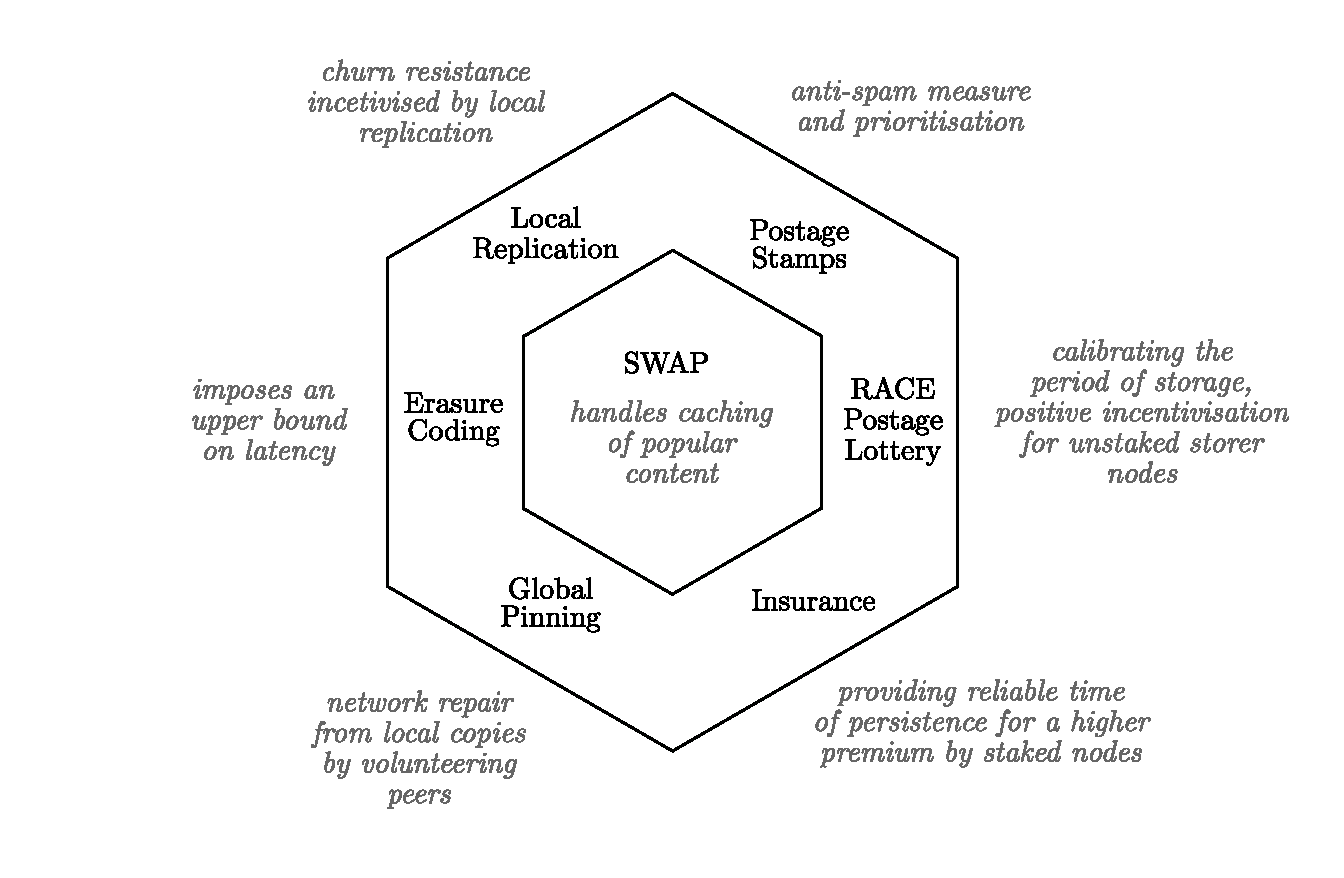
\includegraphics[width=\textwidth]{fig/incentive-design-3.pdf}
\caption[Incentive design \statusgreen]{Incentive design}
\label{fig:incentives}
\end{figure}

% The rest of this chapter is concerned with describing the desired emergent behaviour of the network (\ref{sec:emergent_behavior}), after which we describe the actions which incur costs and those that provide value (\ref{sec:cost_benefit}). Finally, we proceed by describing the incentive mechanisms which ensures that costs are borne as directly as possible by the initiator of the action, with benefits flowing to the nodes who provided the initiator with the expected outcome, ultimately facilitating the desired emergent behavior (see \ref{sec:incentive_mechanisms}).

% \section{Incentive design \statusred}
% \wip{foundational requirement + analysis} 
% \subsection{WIP Desired emergent behavior \statusred}\label{sec:emergent_behavior}
% \subsection{WIP Analysis on expected costs and benefits of actions \statusred}\label{sec:cost_benefit}
% \subsection{WIP Proposed incentive mechanisms \statusred}\label{sec:incentive_mechanisms}
% This section will constitute most of the sections which are already described below.


\section{Sharing bandwidth\statusgreen}

\green{}

\subsection{Incentives for serving and relaying\statusgreen}\label{sec:incentives-relaying}

\green{}

\subsubsection{Forwarding Kademlia and repeated dealings}

Retrieval of a chunk is ultimately initiated by someone accessing content and therefore, all costs related to this retrieval should be borne by them. While paid retrievals may not sound like a popular idea when today's web is "free", many of the problems with the current web stems from consumers' inability to share the costs of hosting and distribution with content publishers directly. In principle, the retrieval of a chunk can be perceived as a functional unit where the storer acts as a service provider and the requestor as consumer. As service is given by provider to consumer, compensation should be given by consumer to provider. Such a direct transaction would normally require that transactors are known to each other, so if we are to maintain the anonymity requirement on downloads, we must conceptualise compensation in a novel way. 

As we use Forwarding Kademlia, chunk retrieval subsumes a series of relaying actions performed by forwarding nodes. Since these are independent actors, it is already necessary to incentivise each act of relaying independently. Importantly, if only instances of relaying are what matters, then, irrespective of the details of accounting and compensation (see \ref{sec:accounting}), transactors are restricted to connected peers. Given the set of ever connected peers is a quasi-permanent set across sessions, this allows us to frame the interaction in the context of repeated dealings. Such a setting always creates extra incentive for the parties involved to play nice. It is reasonable to exercise preference for peers showing untainted historical record. Moreover, since this quasi-permanent set is logarithmic to network size, any book-keeping or blockchain contract that the repeated interaction with a peer might necessitate is kept manageable, offering a scalable solution. Turning the argument around, we could say that keeping balances with a manageable number of peers, as well as the ambiguity of request origination are the very reasons for nodes to have limited connectivity, i.e., that they choose leaner Kademlia bins.

\subsubsection{Charging for backwarded response}

If accepting a retrieve request already constitutes revenue for forwarding nodes, i.e. an accounting event crediting the downstream peer is triggered before the response is delivered, then it creates a perverse incentive not to forward the requests. Conditioning the request revenue fulfilment on successful retrieval is the natural solution: The accounting event is triggered only when a requested chunk is delivered back to its requestor, see figure \ref{fig:retrieval-payment}.


\begin{figure}[htbp]
   \centering
   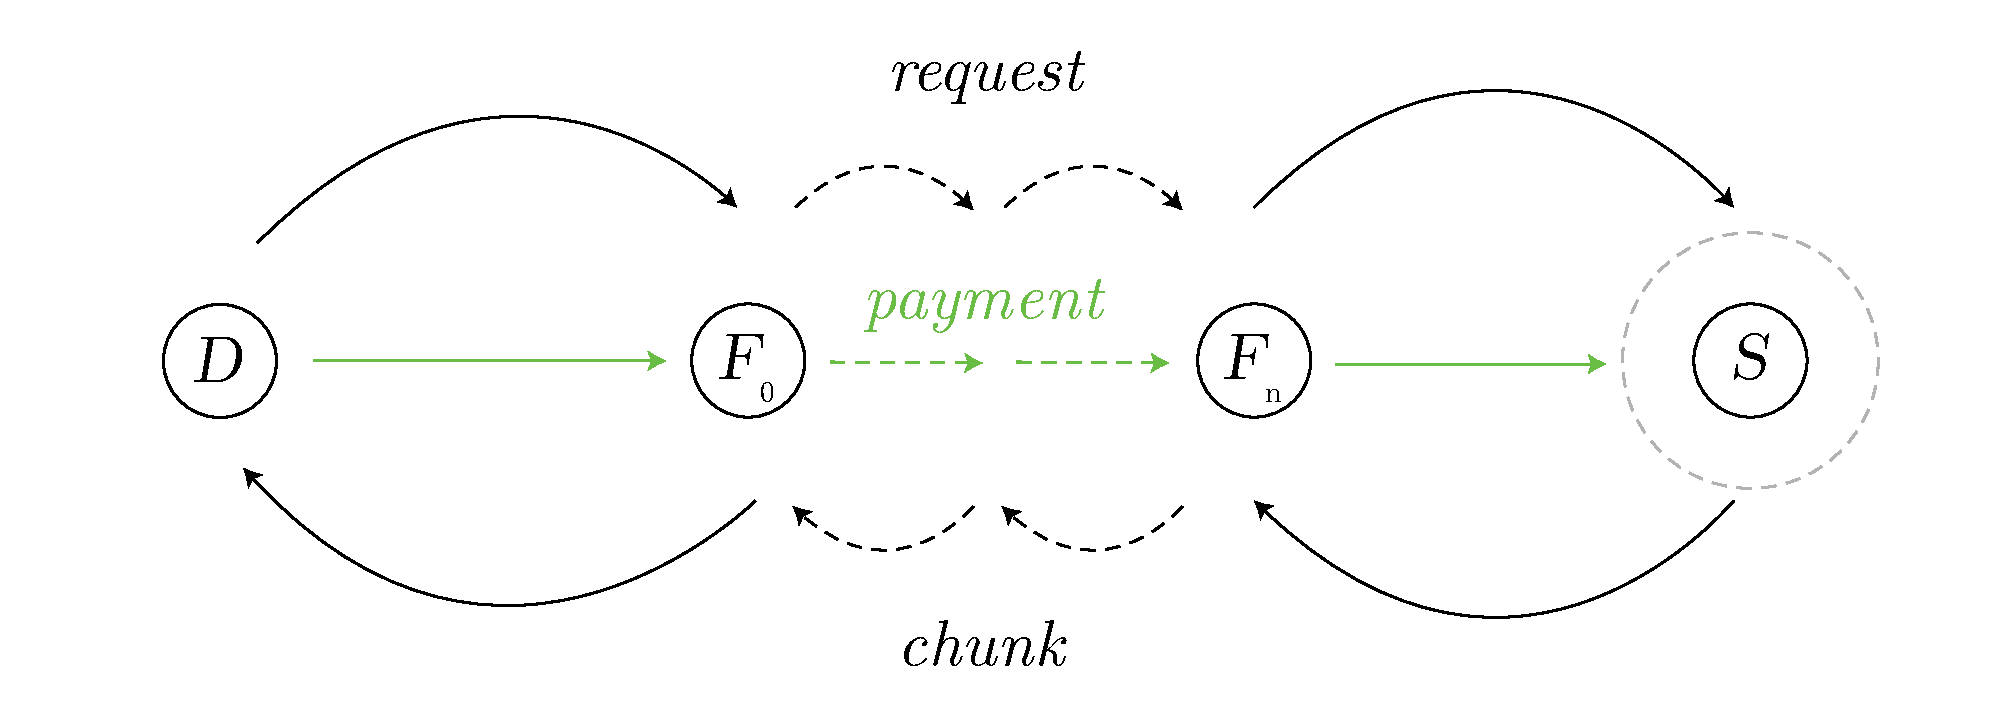
\includegraphics[width=\textwidth]{fig/retrieval-payment.pdf}
   \caption[Incentivising retrieval \statusgreen]{Incentivising retrieval. Node $D$ (Downloader) sends a retrieve request to the chunk's address. Retrieval uses forwarding, so the request is relayed via forwarding nodes $F_0$, ..., $F_n$ all the way to node $S$, the storer node closest to the chunk address. The chunk is delivered by being passed back along the same route to the downloader. Receiving the chunk response triggers an accounting event.}
   \label{fig:retrieval-payment}
\end{figure}

If, however, there is no cost to a request, then sending many illegitimate requests for non-existing chunks (random addresses) becomes possible. This is easily mitigated by imposing sanctions on peers that send too many requests for chunks that do not exist (see \ref{sec:sanctions}).

Once a node initiates (starts or forwards) a request, it commits to pay for that chunk if it is delivered within the defined \gloss{time to live} (\gloss{TTL}), therefore there is never an incentive to block timely deliveries when the chunk is passed back.  This commitment also dissuades nodes from frivolously asking too many peers for a chunk, since, if multiple peers respond with delivery, each must be paid.


\subsection{Pricing protocol for chunk retrieval\statusgreen}\label{sec:pricing}

\green{}

Next, we describe the protocol which nodes use to communicate their price for delivering chunks in the Swarm network. Building on top of this protocol, strategies can then be implemented by nodes who wish to compete in the market with other nodes in terms of quality of service and price (see \ref{spec:strategy:pricing}). 

\subsubsection{Price discovery}\label{sec:retrieval-price-discovery}

The main merit of the protocol is that it allows for the mechanisms of price discovery to be based only on local decisions, which is essential for the following reasons: (1) Bandwidth costs are not homogeneous around the world: Allowing nodes to express their cost structure via their price will enable competition on price and quality, ultimately benefiting the end-user. (2) The demand for bandwidth resource is constantly changing due to fluctuations in usage or connectivity. (3) Being able to react directly to changes creates a self-regulating system. 

Practically, without this possibility, a node operator might decide to shut down their node when costs go up or conversely end-users might overpay for an extended period of time when costs or demand decrease and there is no competitive pressure for nodes to reduce their price accordingly. 

Bandwidth is a service that comes with "instant gratification" and therefore immediate acknowledgement and accounting of its cost are justified. Since it is hard to conceive of any externality or non-linearity in the overall demand and supply of bandwidth, a pricing mechanism which provides for both (1) efficient and immediate signalling, as well as (2) competitive choice with minimal switching and discovery cost, is most likely to accommodate strategies that result in a globally optimal resource allocation.

To facilitate this, we introduce a protocol message that can communicate these prices to upstream peers (see \ref{spec:protocol:retrieval}). We can conceptualise this message as an alternative response to a request. Nodes maintain the prices associated with each peer for each proximity distance, so when they issue a retrieve request they already know the price they commit to pay in the event that the downstream peer successfully delivers the valid chunk within the time to live period. However, there is no point in restricting the price signal just to responses: For whatever reason a peer decides to change the prices, it is in the interest of both parties to exchange this information even if there is request to respond to. In order to prevent DoS attacks by flooding upstream peers with price change messages, the rate of price messages is limited. Well behaved and competitively priced nodes are favoured by their peers; if a node's prices are set too high or their prices exhibit a much higher volatility than others in the network, then peers will be less willing to request chunks from them.%
%
\footnote{While this suggests that unreasonable pricing is taken care of by market forces, in order to prevent catastrophic connectivity changes as a result of radical price fluctuations, limiting the rate of change may need to be enforced on the protocol level. }

For simplicity of reasoning we posit that the default price is zero, corresponding to a free service (altruistic strategy, see \ref{spec:strategy:pricing}). 

\subsubsection{Differential pricing of proximities}\label{sec:diff-pricing-prox}

If the price of a chunk is the same at all proximities, then there is no real incentive for nodes to forward requests other than the potential to cache the chunk and earn revenue by reselling it. This option is hard to justify for new chunks, especially if they are in the shallow proximity orders of a node where they are unlikely to be requested. More importantly, if pricing of chunks is uniform across proximity orders, colluding nodes can generate chunk traffic and pocket exactly as much as they send, virtually a free DoS attack (see figure \ref{fig:ddos-uniform-price}).

\begin{figure}[htbp]
   \centering
   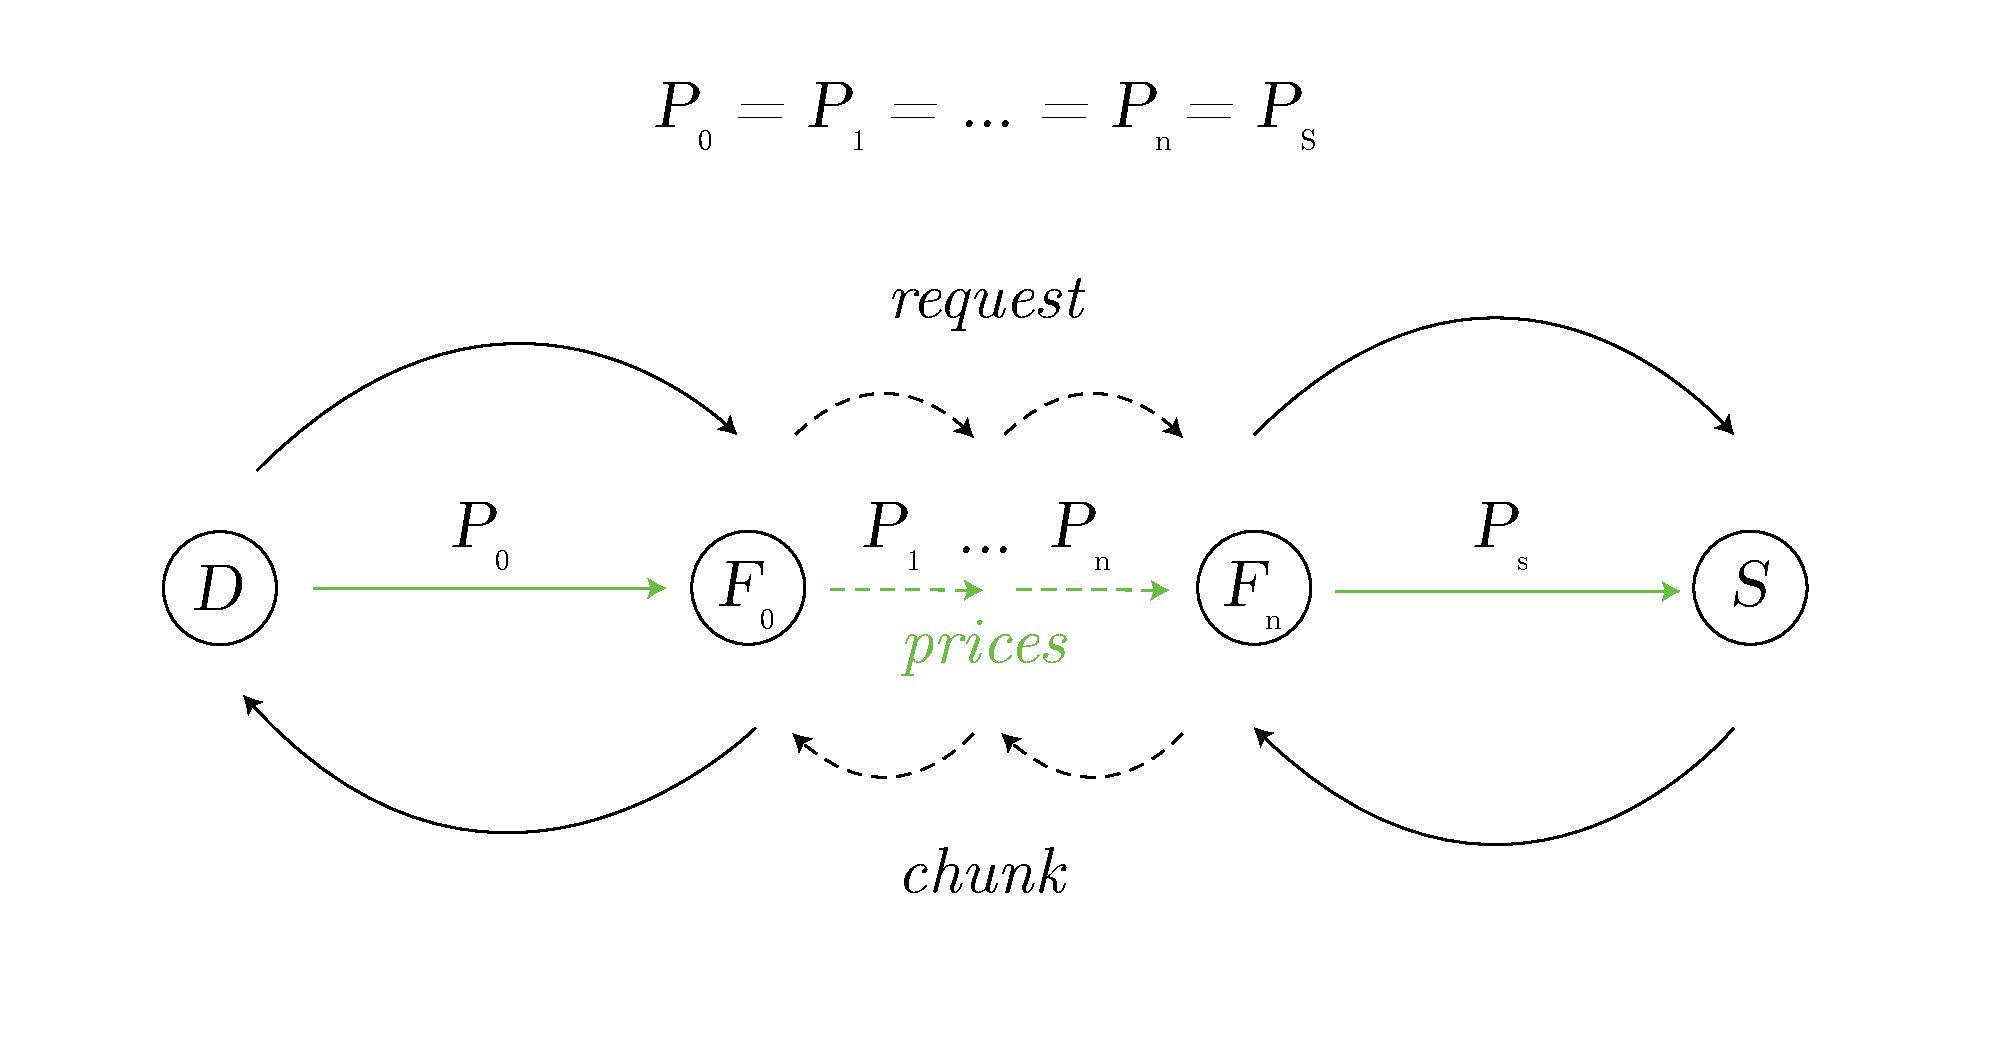
\includegraphics[width=\textwidth]{fig/ddos-uniform-price.pdf}
   \caption[Uniform chunk price across proximities would allow a DoS \statusgreen]{Uniform chunk price across proximities would allow a DoS attack. An attacker can create a flow of traffic between two nodes $D$ and $S$ by sending retrieve requests towards $S$ which only $S$ can serve. If prices are the same across proximities, such an attack would incur no cost for the attacker.}
   \label{fig:ddos-uniform-price}
\end{figure}

To mitigate this attack, the price a requestor pays for a chunk needs to be strictly greater than what the storer node would receive as compensation when a request is routed from requestor to storer. We need to have a pricing scheme that rewards forwarding nodes, hence, this necessitates the need for differential pricing by node proximity. If the price of delivery is lower as a node gets further from the chunk, then the request can always be sent that way because the forwarder will pocket the difference and therefore make a profit. This means that an effective differential scheme will converge to a pricing model where delivery costs more if the peer is further from the chunk address, i.e. rewards for chunk deliveries are a decreasing function of proximity. 

Due to competitive pressure along the delivery path and in the neighborhood, we expect that the differential a node is applying to the downstream price to converge towards the marginal cost of an instance of forwarding.
The downstream price is determined by the bin density of the node. Assuming balanced bins with cardinality $2^n$, a node can guarantee to increase the proximity order by $n$ in one hop. At the same time it also means that they can spread the cost over $n$ proximity bins pushing the overall price down.


\subsubsection{Uniformity of price across peers}

Take a node $A$ that needs to forward a request for a chunk which falls into $A$'s PO bin $n$. Notice that all other peers of $A$ in bins $n+1, n+2, ...$, just like $A$ also have the chunk in their PO $n$. If any of these peers, say $B$, has a price  for proximity order $n$ cheaper than $A$, $A$ can lower its price for PO bin $n$, forward all increased traffic to $B$ and still pocket the difference, see figure  \ref{fig:price-arbitrage}. Note that this is not ideal for the network as it introduces a \gloss{spurious hop} in routing, i.e., in relaying without increasing the proximity. 


\begin{figure}[htbp]
   \centering
   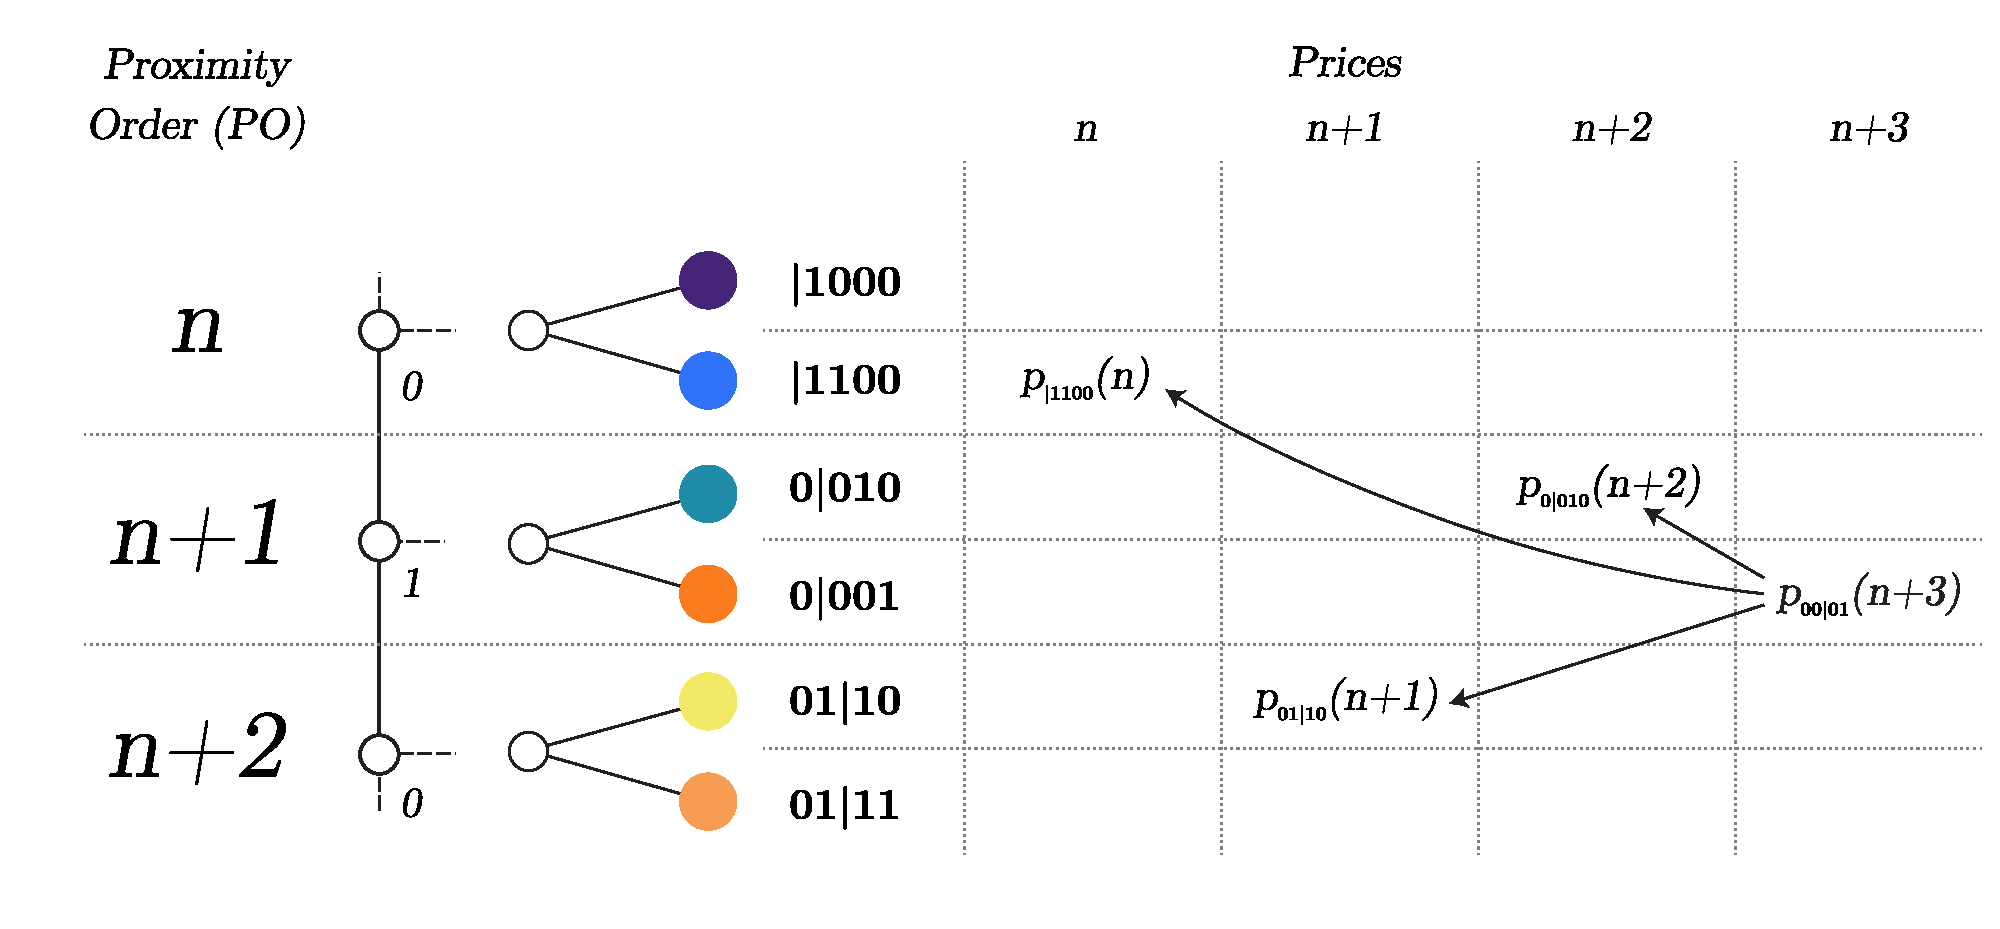
\includegraphics[width=\textwidth]{fig/price-arbitrage-3.pdf}
    \caption[Price arbitrage \statusgreen]{Price arbitrage. Nodes keep a pricetable for prices of every proximity order for each peer. The digaram shows node $0101$ trying to forward a retrieve request for $0000$. The arrows originate from the closest node, and point to cells where other peers although further from the chunk, offer cheaper to forward. Choosing the cheaper peer will direct traffic away from the overpriced peer and lead to a pressure on both to adjust.}
   \label{fig:price-arbitrage}
\end{figure}
 


Similarly, peers of $A$ in shallower bins that have lower price than $A$ for their respective bins, e.g. $B$ in bin $n-1$ is cheaper than $A$ in bin $n$, then $A$ can always forward any request to $B$ and pocket the difference.

Now let's assume that all peers have price tables which are monotonically decreasing as PO decreases. Also assume that shallower bins have higher prices for bins less than $n$ and all deeper peers in bins higher than $n$ have the same prices for $n$. Let $B$, $C$, $D$ and $E$ be the peers in bin $n$ densely balanced. $A$ wants to  forward a chunk to a peer so that the PO with its target address increases by 3. If the peers $B$ and $C$ attempt to collude against $A$ and raise the price of forwarding chunks to bin $n+3$, they are still bound by $D$ and $E$'s price on PO bin $n+2$. In particular if they are lower than $B$ and $C$ for $n+3$.

Such price discrepancies offer nodes an arbitrage opportunity; the strategy to forward to the cheapest peer will direct traffic away from expensive peers and increase traffic for cheaper ones. As a consequence prices will adjust. 

All else being equal, this price arbitrage strategy will achieve (1) uniform prices for the same proximity order across the network, (2) prices that linearly decrease as a function of proximity (3) nodes can increase connectivity and keep prices lower. In this way, incentivisation is designed so that strategies that are beneficial to individual nodes are also neatly aligned in order to benefit the health of the system as a whole.


\subsubsection{Bin density}

Charging based on the downstream peer's proximity to the chunk has the important consequence that the net revenue earned from a single act of non-local delivery to a single requestor is a monotonically increasing function of the difference between the chunk's proximity to the node itself vs to the peer the request was forwarded to. In other words, the more distance we can cover in one forward request, the more we earn. 

This incentive aligns with downloaders' interest to save hops in serving their requests leading to lower latency delivery and less bandwidth overhead. This scheme incentivises nodes to keep a gap-free balanced set of addresses in their Kademlia bins as deep as possible (see figure \ref{fig:bindensity}), i.e, it is better for a node to keep dense Kademlia bins than thin ones.


Nodes that are able to maintain denser bins actually have the same cost as thinner ones, but saving hops will improve latency and make the peer more efficient. This will lead to the peer being preferred over other peers that have the same prices. Increased traffic essentially can also lead to bandwidth contention which eventually allows the raising of prices. 

Note that such arbitrage is more efficient in \glossplural{shallow bin} bins where the number of peers to choose from is higher. This is in major opposition to \glossplural{deep bin} in the area of responsibility. If a node does not replicate its neighbourhoods chunks, some of these chunks will need to be requested by the node closer to the address but further from the node. This will only be possible at a loss. An added incentive for neighbours to replicate their area of responsibility is discussed in \ref{sec:postage-lottery}. With the area of responsibility stored however, a node can choose to set their price arbitrarily. 


\subsubsection{Caching and auto-scaling}\label{sec:caching}

Nodes receive a reward every time they serve a chunk, therefore the profitability of a chunk is proportional to its popularity: the more often a chunk is requested, the higher the reward relative to the fixed cost of storage per time unit. When nodes reach storage capacity limits and it comes to deciding which chunks to delete, the optimal strategy of a rational profit maximising agent is to remove chunks whose profitability is lowest. A reasonably%
%
\footnote{Better metrics for predicting chunk profitability than the age of last request will continue to be identified and developed(see also \ref{spec:strategy:garbage-collection})}.
good predictor for this is the age of last request. In order to maximise the set of chunks to select from, nodes engage in opportunistic caching of the deliveries they relay as well as the chunks they sync. This then results in popular chunks being more widely spread and faster served, making the entire swarm an auto-scaled and auto-balanced \emph{content distribution network}.


\subsubsection{Non-caching nodes}

Any scheme which leaves \glossplural{relaying node} a profit creates a positive incentive for forwarding-only non-caching nodes to enter the network. Such nodes are not inherently beneficial to the network as they are creating unnecessary bandwidth overhead. On the one hand, their presence could in principle unburden storer nodes from relaying traffic, so using them in shallow bins may not be detrimental. On the other hand, closer to neighbourhood depth, their peers will favour a caching/storing node to them because of their disadvantage at least for chunks in their hypothetical area of responsibility. Non-caching nodes can also contribute to increase anonymity (see \ref{sec:retrieval}).

\subsection{Incentivising push-syncing\statusgreen}\label{sec:push-sync-incentives}

\green{}

Push-syncing (see \ref{sec:push-syncing}) is the protocol which ensures that chunks that are uploaded into the network arrive at their proper address. In what follows, we will explain how forwarding is incentivised.
%
%
\footnote{To complement our solution for bandwidth compensation, further measures are needed for spam protection and storage incentivisation which are discussed later in \ref{sec:postage-stamps} and \ref{sec:postage-lottery}, respectively.}



The push-sync protocol is analogous to the retrieval protocol in the sense that their respective message exchange sequences travel the same route.
The delivery of the chunk in the push sync protocol is analogous to a retrieval request and, conversely, the statement of custody receipt in push sync is analogous to the chunk delivery response in retrieval.

Push-syncing could in principle be left without explicit forwarding incentives. Due to the retrieval protocol, as nodes expect chunks to be found in the neighbourhood of   their address, participants in swarm are at least weakly incentivised to help uploaded chunks get to their destination by taking part in the protocol. However, we  need to provide the possibility that chunks are uploaded via nodes further from it than the requestor (light  nodes or retries). Thus, if push-syncing was free, nodes could generate wasteful amounts of bandwidth. 

Requiring payment only for push-sync delivery by the downstream peers would put the forwarder in a position to bargain with a storer node on the delivery of the chunk. The possession of a chunk is valuable for the prospective storer node because there is also a system of rewards for storage ( see \ref{sec:postage-lottery}). Given this, the forwarder node could in theory hold onto the chunk unless the storer node pays marginally more than what the possession of this chunk is worth for them factoring in the profit potential due to storage incentives. In particular, since forwarders on the route from the uploader are not numerous, any profit coming from a reward mechanism for storage could then be captured by the forwarding nodes.

Instead, in push-sync, by making the statement of custody receipt a paid message, roles switch. Now, a forwarder node is not in the position to bargain. To see why, consider what would happen if a forwarding node tries to hold on to a chunk to get a price for pushing this chunk to a storer node. In this case, the uploader will not get a statement of custody receipt in due time, assume the attempt has failed and re-upload the chunk via a different route. Now, suddenly the original forwarding node is forced to compete with another forwarding node in getting compensation for their bandwidth costs. Since all forwarding nodes know this, emergent behavior will produce a series of peers that are willing to forward the chunk to the storer node for a only small compensation and the bandwidth costs incurred. Now there is no need for the original forwarding node to try and bargain with the storer node in the first place: Instead, they can make a small profit immediately when they pass back the statement of custody receipt. 


\begin{figure}[htbp]
\centering
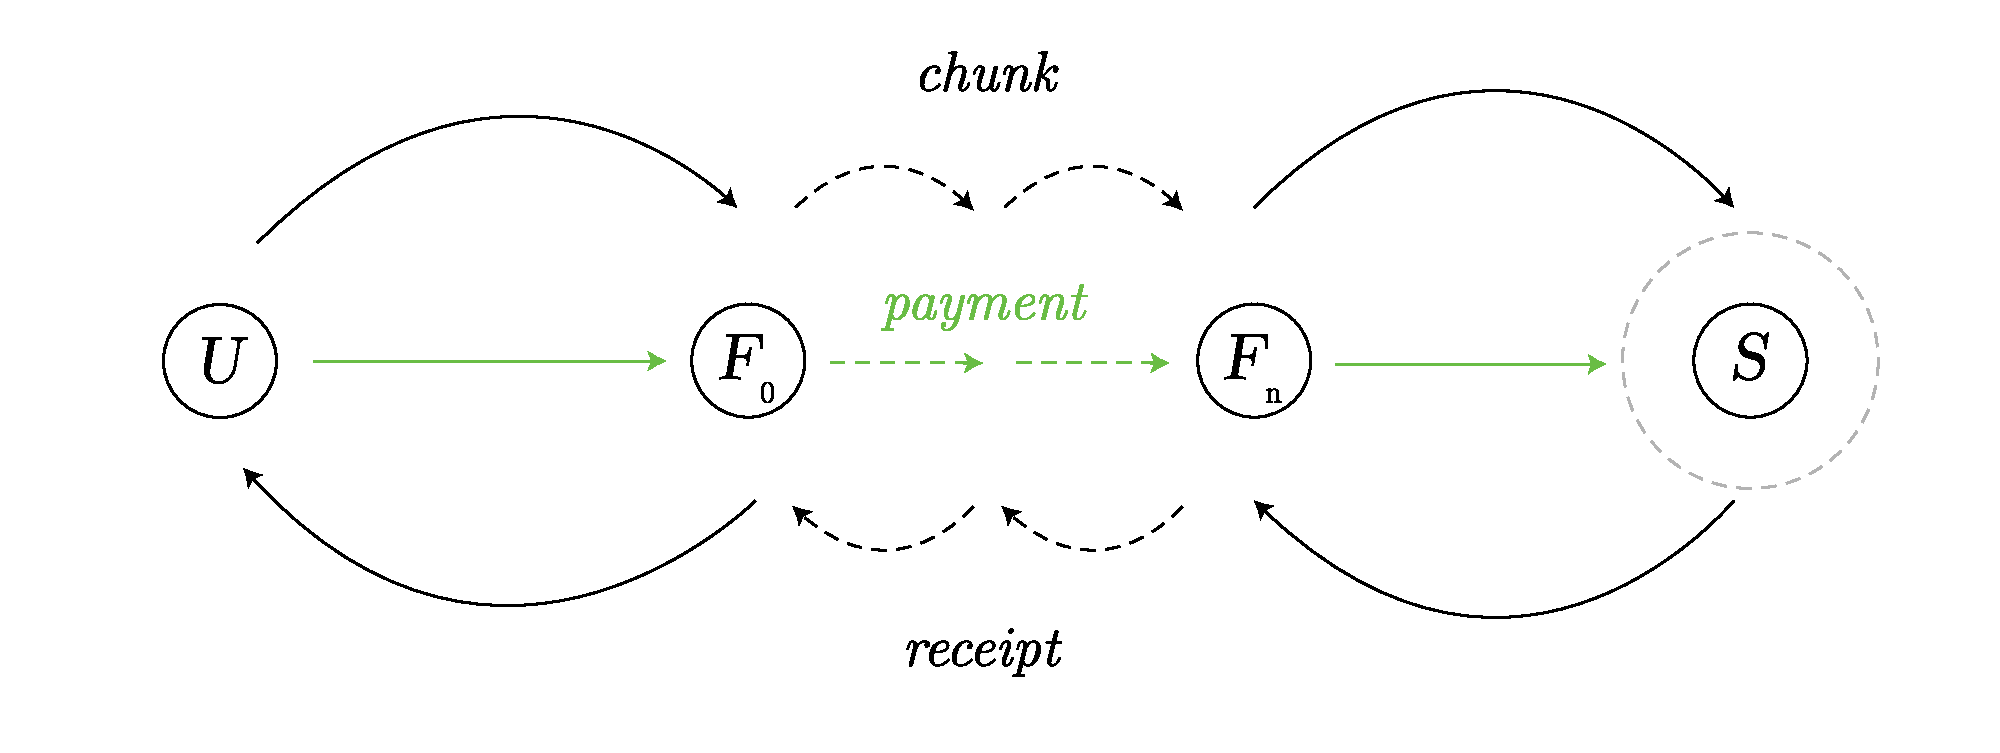
\includegraphics[width=\textwidth]{fig/push-payment.pdf}
\caption[Incentives for push-sync protocol \statusgreen]{Incentives for push-sync protocol. Node $U$ (uploader) sends the chunk towards its address, the closest node to which is node $S$ (storer) via forwarding nodes $F_0, \ldots F_n$. The storer node responds with a statement of custody receipt which is passed back to the uploader via the same forwarding nodes $F_n, \ldots F_0$. Receiving the statement of custody receipt triggers an accounting event.}
\label{fig:syncing-swap}
\end{figure}

This scheme makes it clear why the incentivisation of the two protocols relies on the same premises: there are many sellers (forwarders) and only one buyer (uploader) for a homogeneous good (the statement of custody receipt). This drives the price of the service (delivering the chunk to the storer) to the sum of all marginal cost of forwarding for each node along the route, while simultaneously allowing the storer node to capture all profits from the storage compensation scheme.

In this way, we can make sure that (1) storers actually respond with receipts, and (2) have a way to detect timed out or unsolicited receipt responses to protect against DoS, see figure \ref{fig:syncing-swap}.

Just as in the retrieval protocol, the pricing is expected to be different for different proximities (see \ref{sec:diff-pricing-prox} and as the costs of the nodes in the network change (depending on capacity utilization and efficiency of nodes), the pricing will be variable over time as well. Since at the point of accounting the compensation is due for one chunk and one shorter message (retrieve request and custody receipt), we can safely conclude that the price structure for forwarding in the case of the two protocols are identical and therefore one generic forwarding pricing scheme can be used for both (see  \ref{sec:retrieval-price-discovery}) 
What makes a difference is that unlike the retrieval protocol where the chunk is delivered back and its integrity can be validated, the accounting event in pushsync is a statement of custody which can be spoofed. With the forwarding incentive nodes will have the motivation not to forward and impersonate a storer node and issue the statement of  custody. This makes it advisable to query (retrieve) a chunk via alternative routes. If  such  retrievals fail, it may be necessary to try to push-sync chunks via alternative routes. 
 

\section{Swap: accounting and settlement\statusgreen}\label{sec:accounting-and-settlement}

\green{}

This section covers aspects of incentivisation relating to bandwidth sharing. 
In \ref{sec:accounting}, we introduce a mechanism to keep track of the data traffic between peers and offer peer to peer accounting for message relaying.
Subsequently, in \ref{sec:cheques}, we describe the conditions of compensating for unbalanced services and show how settlement can be achieved.
In particular we introduce the concept of a. \glossplural{cheque} and the \gloss{chequebook contract}. In \ref{sec:waiver}, we discuss waivers, a further optimisation allowing for more savings on transaction cost. In \ref{sec:zero-cash-entry} we discuss how an incentivised service of sending in cashing transactions enables zero-cash entry to Swarm and, finally, in \ref{sec:sanctions} we will discuss the basic set of sanctions that serve as a fundamental incentive for nodes to play nice and adhere to the protocols.

\subsection{Peer to peer accounting\statusgreen}\label{sec:accounting}


\cite{ethersphere2016sw3} introduces a protocol for peer-to-peer accounting, called \gloss{swap}. Swap is a tit-for-tat accounting scheme that scales microtransactions (see \ref{spec:protocol:swap}). The scheme allows directly connected peers to swap payments or payment commitments. The major features of the system are captured playfully with different mnemonic resolutions of the acronym SWAP:

\begin{itemize}
    \item \emph{Swarm accounting protocol} for \emph{service wanted and provided} -- Account service for service exchange.
    \item \emph{settle with automated payments} -- Send \gloss{cheque} when \gloss{payment threshold} is exceeded.
    \item \emph{send waiver as payment} -- Debt can be waived in the value of un-cashed cheques. 
    \item \emph{start without a penny} and \emph{send with a peer} -- Zero cash entry is supported by unidirectional swap.
\end{itemize}

\subsubsection{Service for service}

\gloss{swap} allows service for service exchange between connected peers. In case of equal consumption with low variance over time, bidirectional services can be accounted for without any payments. Data relaying is an example of such a service, making Swap ideally suited for implementing bandwidth incentives in content delivery or mesh networks.

\begin{figure}[htbp]

\begin{center}
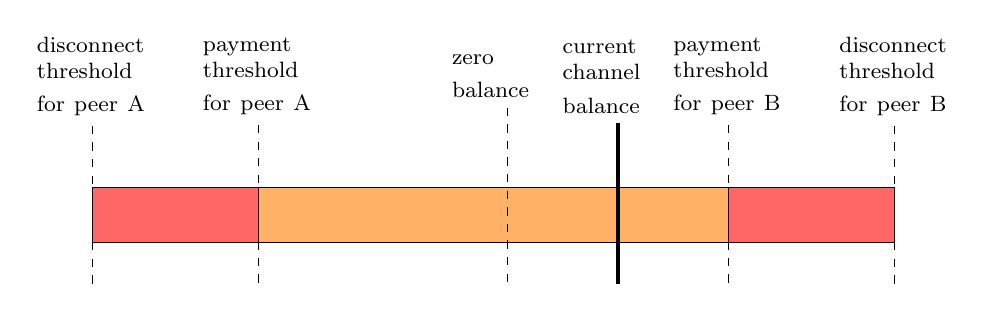
\begin{tikzpicture}
\node (middle)[draw, rectangle, fill=orange!60, minimum height=2em, minimum width=18em]{};
\node (leftred) [draw, rectangle, fill=red!60, minimum height=2em, minimum width=6em, node distance=12em,left of=middle]{};
\node (rightred)[draw, rectangle, fill=red!60, minimum height=2em, minimum width=6em, node distance=11em,right of=middle]{};
\node (zero) [above of=middle,node distance=5em, text width=4em, align=left] {\footnotesize zero\\ balance};
\node (zerod) [below of=middle] {};
\draw [dashed](zero)--(zerod);
\node (rtol) [node distance=8em,right of=zero,text width=4em, align=left] {\footnotesize payment\\threshold\\for peer B};
\node (rtold) [node distance=8em,right of=zerod] {};
\node (ltol) [node distance=9em,left of=zero,text width=4em, align=left] {\footnotesize payment\\threshold\\for peer A};
\node (ltold) [node distance=9em,left of=zerod] {};
\node (rdis) [node distance=14em, right of=zero,text width=4em, align=left] {\footnotesize disconnect\\threshold\\for peer B};
\node (rdisd) [node distance=14em,right of=zerod] {};
\node (ldis) [node distance=15em, left of=zero,text width=4em, align=left] {\footnotesize disconnect\\threshold\\for peer A};
\node (ldisd) [node distance=15em,left of=zerod] {};
\node (rbal) [node distance=4em,right of=zero,text width=4em, align=left] {\footnotesize current\\channel\\balance};
\node (rbald) [node distance=4em,right of=zerod] {};

\draw [dashed](rtol)--(rtold);
\draw [dashed](ltol)--(ltold);
\draw [dashed](rdis)--(rdisd);
\draw [dashed](ldis)--(ldisd);
\draw [very thick](rbal)--(rbald);
\end{tikzpicture}
\end{center}
\caption[Swap balance and swap thresholds \statusgreen]{Swap balance and swap thresholds.
Zero balance in the middle indicates consumption and provision are equal.
The current channel balance represents the difference in uncompensated service provision:
If to the right of zero, the balance tilts in favour of A with peer B being in debt, whereas to the left
the balance tilts in favour of B with A being in debt.
The orange interval represents loss tolerance. If the balance goes over the payment threshold, the party in
debt sends a \gloss{cheque} to its peer, if it reaches the \gloss{disconnect threshold}, the peer in debt is disconnected.}
\label{fig:swap}
\end{figure}

\subsubsection{Settling with payments}

In the presence of high variance or unequal consumption of services, the balance will eventually tilt significantly toward one peer. In this situation, the indebted party issues a payment to the creditor to return the nominal balance to zero. This process is automatic and justifies swap as \emph{settle (the balance) with automated payments} (see figure \ref{fig:swap}). These payments can be just commitments.


\subsubsection{Payment thresholds}

To quantify what counts as "significant tilt", the swap protocol requires peers to advertise a \gloss{payment threshold} as part of the handshake (\ref{spec:protocol:swap}): When their relative debt to their peer goes above this threshold, they send a message, containing a payment to their peer. It is reasonable for any node to send a message at this level, as there also exist a disconnect threshold. The disconnect threshold is set freely by any peer, but a reasonable value is such that the difference between the payment threshold and the disconnect threshold accounts for the normal variance in accounting balances of the two peers.   (see \ref{spec:strategy:swap}). 


\subsubsection{Atomicity}

Sending the \gloss{cheque} and updating the balance on the receiving side cannot be made an atomic operation without substantial added complexity. For instance, a client could crash between receiving and processing the message, so even if the sending returns with no error, the sending peer can not be sure the payment was received, this can result in discrepancies in accounting on both sides. The tolerance expressed by the difference between the two thresholds ($\mathit{DisconnectThreshold}-\mathit{PaymentThreshold}$) guards against this, i.e. if the incidence of such crashes is not high and happen with roughly equal probability for both peers, the resulting minor discrepancies are filtered out. In this way, the nodes are shielded from sanctions.

\begin{center}
\begin{figure}[htbp]

\begin{center}
\begin{tabular}{ccc}
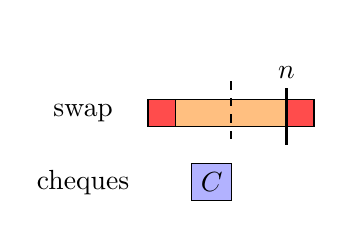
\begin{tikzpicture}
\node (middle)[draw, rectangle, fill=orange!50, minimum height=1em, minimum width=4em]{};
\node (leftred) [draw, rectangle, fill=red!70, minimum height=1em, minimum width=1em, node distance=2.5em, left of=middle]{};
\node (rightred)[draw, rectangle, fill=red!70, minimum height=1em, minimum width=1em, node distance=2.5em, right of=middle]{};
\node (zero) [above of=middle,node distance=2em, text height=1em] {};
\node (zerod) [below of=zero, node distance=3.5em] {};
\node (balance) [right of=zero,node distance=2em, text height=1.5em] {$n$};
\node (balanced) [below of=balance,node distance=3.5em] {};
\draw [dashed](zero)--(zerod);
\draw [very thick](balance)--(balanced);
\node (payment) [below of=zerod, node distance=1em]{};
\node (cheqeue) [draw, left of=payment, node distance=.7em, minimum height=1em, minimum width=1.4em, fill=blue!30, rectangle]{$C$};

\node (swap) [left of=leftred,minimum width=1em,align=right]{swap};
\node (cheques) [below of=swap,minimum width=1em, node distance= 2.5em, align=right]{cheques};
\end{tikzpicture}
&
\begin{tabular}{c}
  $\Longrightarrow$
\\ \\ \\ \\
\end{tabular}
&
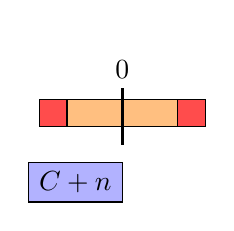
\begin{tikzpicture}
\node (middle)[draw, rectangle, fill=orange!50, minimum height=1em, minimum width=4em]{};
\node (leftred) [draw, rectangle, fill=red!70, minimum height=1em, minimum width=1em, node distance=2.5em, left of=middle]{};
\node (rightred)[draw, rectangle, fill=red!70, minimum height=1em, minimum width=1em, node distance=2.5em, right of=middle]{};
\node (zero) [above of=middle,node distance=2em, text height=1.5em] {$0$};
\node (zerod) [below of=zero, node distance=3.5em] {};
% \draw [dashed](zero)--(zerod);
\draw [very thick](zero)--(zerod);
\node (payment) [below of=zerod, node distance=1em]{};
\node (cheque) [draw, left of=payment, node distance=1.7em, minimum height=1em, minimum width=3.4em, fill=blue!30, rectangle]{$C+n$};
\end{tikzpicture}
\end{tabular}
\end{center}

\caption[Cheque swap \statusgreen]{Peer B's swap balance (with respect to A) reaches the payment threshold (left),
B sends a cheque to peer A. B keeps the cheque and restores the swap balance to zero.}
\label{fig:chequeswap}
\end{figure}
\end{center}

\subsection{Cheques as off-chain commitments to pay\statusgreen}\label{sec:cheques}

One of the major issues with direct \gloss{on-chain payment} in a blockchain network is that each transaction must be processed by each and every node participating in the network, resulting in high transaction costs. It is however, possible to create a payment without presenting this payment on-chain. Such payments are called \gloss{second-layer payment} strategies. One such strategy is to defer payments and process them in bulk. In exchange for reduced cost, the beneficiary must be willing to incur higher risk of settlement failure. We argue that this is perfectly acceptable in the case of bandwidth incentivisation in Swarm, where peers will engage in repeated dealings.


\subsubsection{The chequebook contract}

A very simple smart contract that allows the beneficiary to choose when payments are to be processed was introduced in \cite{ethersphere2016sw3}. This \gloss{chequebook contract} is a wallet that can process \glossplural{cheque} issued by its owner. These cheques are analogous to those used in traditional financial transactions: The issuer signs a \emph{cheque} specifying a \emph{beneficiary}, a \emph{date} and an \emph{amount}, gives it to the recipient as a token of promise to pay at a later date. The smart contract plays the role of the bank. When the recipient wishes to get paid, they "cash the cheque" by submitting it to the smart contract. The contract, after validating the signature, date and the amount specified on the cheque, transfers the amount to the beneficiary's account (see figure \ref{fig:swap-chequebook}). Analogous to the person taking the cheque to the bank to cash it, anyone can send the digital cheque in a transaction to the owner's chequebook account and thus trigger the transfer. 

The swap protocol specifies that when the \emph{payment threshold} is exceeded, a cheque is sent over by the creditor peer. Such cheques can be cashed immediately by being sent to the issuer's chequebook contract. Alternatively, cheques can also be held. Holding a cheque is effectively lending on credit, which enables the parties to save on transaction costs. 

The amount deposited in the chequebook (\gloss{global balance}) serves as collateral for the cheques. It is pooled over the beneficiaries of all outstanding cheques. In this simplest form, the chequebook has the same guarantee as real-world cheques: None. Since funds can be freely moved out of the chequebook wallet at any time, solvency at the time of cashing can never be guaranteed: If the chequebook's balance is less than the amount sanctioned by a cheque submitted to it, the cheque will bounce. This is the trade off between transaction costs and risk of settlement failure.

While, strictly speaking, there are no guarantees for solvency, nor is there an explicit punitive measure in the case of insolvency, a bounced cheque will affect the issuer's reputation as the chequebook contract records it. On the premise that cheques are swapped in the context of repeating dealings, peers will refrain from issuing cheques beyond their balance. In other words, a node's interest in keeping a good reputation with their peers serves as a incentive enough to maintain its solvency.


\begin{figure}[htbp]
\centering
% Agents
\def\IssuerLocal{A client}
\def\IssuerSwapContract{A swap}
\def\BeneficiarySwapContract{B swap}
\def\BeneficiaryLocal{B client}

% Message Flows
\def\Issue{issue cheque}% \def\Cheque{Cheque}
\def\Redeem{redeem cheque} %\def\Cheque{Cheque}
\def\Clear{clear ETH} %\def\ETH{ETH}
\def\NW{withdrawal event} %\def\Msg{Log Event}
\def\ND{deposit event} %\def\Msg{Log Event}

% Legend 
\def\LegendOnChain{On-chain}
\def\LegendOffChain{Off-chain}


\begin{tikzpicture}[every node/.style={font=\small,
  minimum height=.35cm,minimum width=.5cm},]

%
% Matrix
\node [matrix, very thin,column sep=1.0cm,row sep=0.2cm] (matrix) at (0,0) {
  & \node(0,0) (\IssuerLocal) {};   &                         & \node(0,0) (\IssuerSwapContract) {};   & & \node(0,0) (\BeneficiarySwapContract) {};   & & \node(0,0) (\BeneficiaryLocal) {}; \\
  & & & & & & & \\
  & & & & & & & \\
  & & & & & & & \\
  & \node(0,0) (\IssuerLocal 1) {}; & \node(0,0) (\Issue) {}; & \node(0,0) (\IssuerSwapContract 1) {}; & & \node(0,0) (\BeneficiarySwapContract 1) {}; & & \node(0,0) (\BeneficiaryLocal 1) {}; \\
  & & & & & & & \\
  & & & & & & & \\
  & \node(0,0) (\IssuerLocal 2) {}; &                         & \node(0,0) (\IssuerSwapContract 2) {}; & & \node(0,0) (\BeneficiarySwapContract 2) {}; & \node(0,0) (\Redeem) {};  &  \node(0,0) (\BeneficiaryLocal 2) {}; \\ 
  & & & & & & & \\
  & & & & & & & \\
  & \node(0,0) (\IssuerLocal 3) {}; &                         & \node(0,0) (\IssuerSwapContract 3) {}; & \node(0,0) (\Clear) {}; & \node(0,0) (\BeneficiarySwapContract 3) {}; &                    ; & \node(0,0) (\BeneficiaryLocal 3) {}; \\
  & & & & & & & \\
  & \node(0,0) (\IssuerLocal 4) {}; & \node(0,0) (\NW) {}   ; & \node(0,0) (\IssuerSwapContract 4) {}; &                         & \node(0,0) (\BeneficiarySwapContract 4) {}; & \node(0,0) (\ND) {}; & \node(0,0) (\BeneficiaryLocal 4) {}; \\
  & & & & & & & \\
  & \node(0,0) (\IssuerLocal 5) {}; &                         & \node(0,0) (\IssuerSwapContract 5) {};  & & \node(0,0) (\BeneficiarySwapContract 5) {};& & \node(0,0) (\BeneficiaryLocal 5) {}; \\
  & & & & & & & \\
  & \node(0,0) (\IssuerLocal 6) {}; &                         & \node(0,0) (\IssuerSwapContract 6) {};  & & \node(0,0) (\BeneficiarySwapContract 6) {};& & \node(0,0) (\BeneficiaryLocal 6) {}; \\
  & & & & & & & \\
  & \node(0,0) (\IssuerLocal 7) {}; & \node(0,0) (\LegendOnChain) {};  & & & & & \\
  & \node(0,0) (\IssuerLocal 8) {}; & \node(0,0) (\LegendOffChain) {}; & & & & & \\
};

% Agents labels
\fill 
	(\IssuerLocal) node[draw,fill=white] {\IssuerLocal}
	(\IssuerSwapContract) node[draw,fill=white] {\IssuerSwapContract}
	(\BeneficiarySwapContract) node[draw,fill=white] {\BeneficiarySwapContract}
	(\BeneficiaryLocal) node[draw,fill=white] {\BeneficiaryLocal};

\draw [dashed] 
  (\IssuerLocal) -- (\IssuerLocal 6)
  (\BeneficiaryLocal) -- (\BeneficiaryLocal 6)
  (\IssuerSwapContract) -- (\IssuerSwapContract 6)
  (\BeneficiarySwapContract) -- (\BeneficiarySwapContract 6);

% Horizontal flows (Monetary interactions)
%\draw [-latex] (\IssuerLocal 1) -- (\IssuerSwapContract 1.west) arc(180:0:0.37cm) -- (\BeneficiarySwapContract 1.west) arc(180:0:0.37cm) -- (\BeneficiaryLocal 1);
\draw [-{Latex[length=1.5mm,width=2.5mm]}] (\IssuerLocal 1) -- (\BeneficiaryLocal 1);
\draw [-{Latex[length=1.5mm,width=2.5mm]}] (\BeneficiaryLocal 2) -- (\IssuerSwapContract 2);
%\draw [-latex] (\BeneficiaryLocal 2) -- (\BeneficiarySwapContract 2.east) arc(0:180:0.37cm) -- (\IssuerSwapContract 2);
\draw [-{Latex[length=1.5mm,width=2.5mm]}] (\IssuerSwapContract 3) -- (\BeneficiarySwapContract 3);
\draw [-{Latex[length=1.5mm,width=2.5mm]}] (\IssuerSwapContract 3) -- (\IssuerLocal 4);
\draw [-{Latex[length=1.5mm,width=2.5mm]}] (\BeneficiarySwapContract 3) -- (\BeneficiaryLocal 5);

% Flows Labels 
\fill
  (\Issue) 
    node[above, font=\footnotesize ] {\Issue}
  (\Redeem) 
    node[above, font=\footnotesize] {\Redeem}
  (\Clear) 
    node[above, font=\footnotesize] {\Clear}
  (\NW) 
    node[above, font=\footnotesize, text width=1.4cm, text height=1.5cm, align=center,fill=white] {\NW}
  (\ND) 
    node[above, font=\footnotesize, text width=1.5cm,align=center,fill=white] {\ND};

% Interaction points 
\draw 
  (\IssuerLocal 1) node[minimum size=0.25cm, draw,circle,fill=red!20] {}
  (\BeneficiaryLocal 1) node[minimum size=0.25cm, draw,circle,fill=red!20] {}
  (\BeneficiaryLocal 2) node[minimum size=0.25cm, draw,circle,fill=red!20] {}
  (\IssuerSwapContract 2) node[minimum size=0.25cm, draw,circle,fill=green!20] {}
  (\IssuerSwapContract 3) node[minimum size=0.25cm, draw,circle,fill=green!20] {}
  (\IssuerLocal 4) node[minimum size=0.25cm, draw,circle,fill=red!20] {}
  (\BeneficiarySwapContract 3) node[minimum size=0.25cm, draw,circle,fill=green!20] {}
  (\BeneficiaryLocal 5) node[minimum size=0.25cm, draw,circle,fill=red!20] {}
  (\IssuerLocal 7) node[minimum height=.1cm, minimum size=0.1cm, draw,circle,fill=green!20] {}
  (\IssuerLocal 8) node[minimum height=.1cm, minimum size=0.1cm, draw,circle,fill=red!20] {};

% Vertical lifelines
\draw [-{Latex[length=1.5mm,width=2mm]}] (\IssuerSwapContract 2) -- (\IssuerSwapContract 3);
 Legend labels
\draw
	(\LegendOnChain) node[minimum height=.1cm] {\LegendOnChain}
	(\LegendOffChain) node[minimum height=.1cm] {\LegendOffChain};
\end{tikzpicture}

\caption[The basic interaction sequence for swap chequebooks \statusgreen]{The basic interaction sequence for swap chequebooks}
\label{fig:swap-chequebook}
\end{figure}


\subsubsection{Double cashing}

Since these digital cheques are files and can therefore be copied, care must be taken that the same cheque cannot be cashed twice. Such "double cashing" can be prevented by assigning each cheque given to a particular beneficiary a serial number which the contract will store when the cheque is cashed. The chequebook contract can then rely on the serial number to make sure cheques are cashed in sequential order, thus needing to store only a single serial number per beneficiary.

An alternative strategy to prevent double cashing, when repeated payments are made to the same beneficiary, is that the cheques contain the \emph{cumulative} total amount ever credited to the beneficiary. The total amount that has been cashed out is stored in the contract for each beneficiary. When a new cheque is submitted, the contract ignores cheques with amount equal to or less than the stored total, but it will transfer the difference if it receives a cheque with a higher total.


This simple trick also makes it possible to cash cheques in bulk because only the current "last cheque" need ever be processed. This achieves the reduction of transaction costs alluded to above.

\subsubsection{Cashing without Ether}\label{sec:zero_eth}
Not all peers in Swarm are expected to have the Ether needed to pay for the transaction costs to cash out a cheque. The chequebook allows third parties to cash cheques. The sender of the transaction is incentivised with a reward for the service performed.

\subsection{Waivers\statusgreen}\label{sec:waiver}

If the imbalance in the swap channel is the result of high variance as opposed to unequal consumption, after a period of accumulating cheques the channel balance starts tilting the other way. Normally, it is now up to the other party to issue cheques to its peer resulting in un-cashed cheques accumulating on both sides.
To allow for further savings in transaction costs, it could be desirable to be able to "play the cheques off against each other".

Such a process is possible, but it requires certain important changes within the chequebook contract. In particular, cashing cheques can no longer be immediate and must incur a security delay, a concept familiar from other payment channel implementations. 

Let us imagine a system analogous to cheques being returned to the issuer. Assume peer $A$ issued cheques to $B$ and the balance was brought back to zero. Later the balance tilts in $A$'s favour but the cheques from $A$ to $B$ have not been cashed. In the traditional financial world, user B could either simply return the last cheque back to $A$ or provably destroy it. In our case it is not so simple; we need some other mechanism by which $B$ \emph{commits not to cash} that particular cheque. Such a commitment could take several forms; it could be implemented by $B$ signing a message allowing $A$ to issue a new `last cheque` which has a lower cumulative total amount than before, or perhaps $B$ could issue some kind of `negative` cheque for A's chequebook that would have the effect as if a cheque with the same amount had been paid. 

What all these implementations have in common, is that the chequebook can no longer allow instantaneous cashing of cheques. Upon receiving a cheque cashing request, the contract must wait to allow the other party in question to submit potentially missing information about cancelled cheques or reduced totals. To accommodate (semi-)bidirectional payments using a single chequebook we make the following modifications:

\begin{enumerate}
    \item All cheques from user A to user B must contain a serial number.
    \item Each new cheque issued by A to B must increase the serial number.
    \item A's chequebook contract records the serial number of the last cheque that B cashed.
    \item During the cashing delay, valid cheques with higher serial number supersede any previously submitted cheques regardless of their face value.
    \item Any submitted cheque which decreases the payout of the previously submitted cheque is only valid if it is signed by the beneficiary.
\end{enumerate}


\begin{figure}[htbp]
\centering
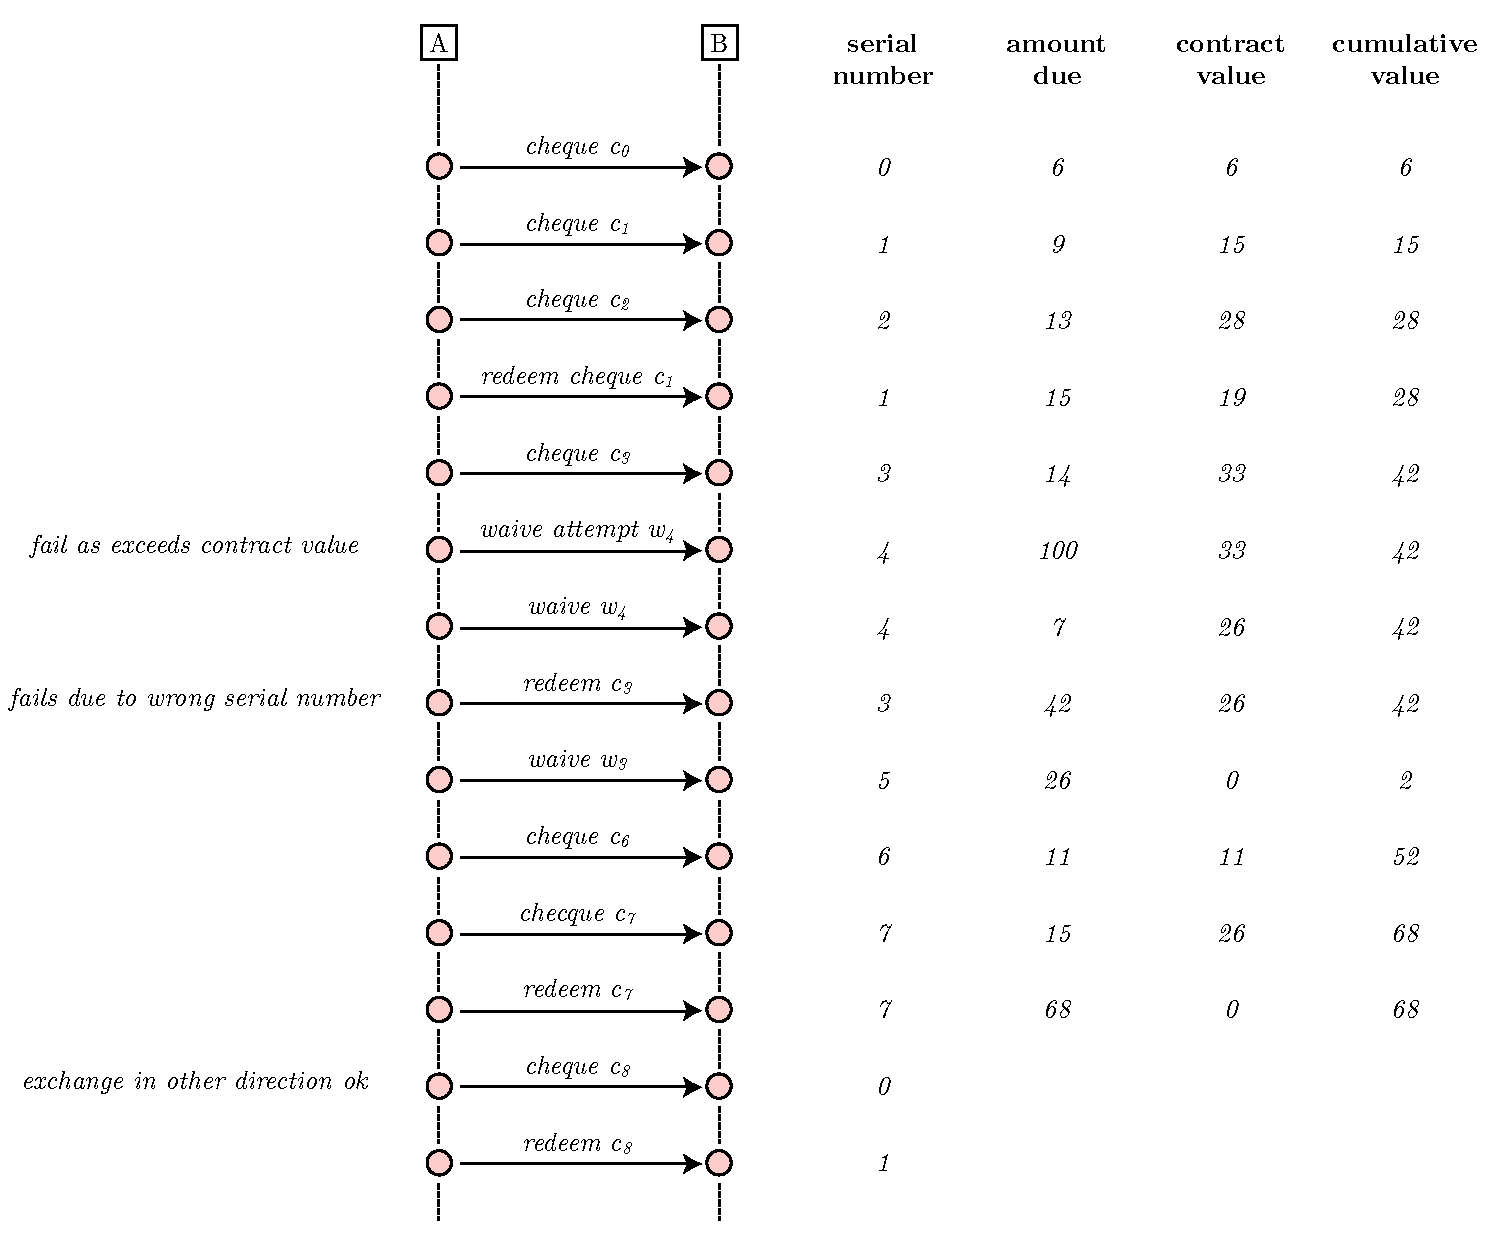
\includegraphics[width=\textwidth]{fig/waivers-diagram-2.pdf}
\caption[Example sequence of mixed cheques and waivers exchange \statusgreen]{Example sequence of mixed cheques and waivers exchange}
\label{fig:waivers-diagram}
\end{figure}

With these rules in place it is easy to see how cheque cancellation would work. Suppose user $A$ has issued cheques $c_0 \ldots c_n$ with cumulative totals $t_0 \ldots t_n$ to user $B$. Suppose that the last cheque $B$ cashed was $c_i$. The chequebook contract has recorded that $B$ has received a payout of $t_i$ and that the last cheque cashed had serial number $i$.

Let us further suppose that the balance starts tilting in $A$'s favour by some amount $x$. If $B$ had already cashed cheque $c_n$, then $B$ would now have to issue a cheque of her own using $B$'s chequebook as the source and naming $A$ as the beneficiary. However, since cheques $c_{i+1} \ldots c_n$  are un-cashed, $B$ can instead send to $A$ a cheque with $A$'s chequebook as the source, $B$ as the beneficiary, with serial number $n+1$ and cumulative total $t_{n+1} = t_n - x$. Due to the rules enumerated above, A will accept this as equivalent to a payment of amount $x$ by $B$.  In this scenario, instead of sending a cheque to $A$, $B$ waives part of their earlier entitlement. This justifies SWAP as \emph{send waiver as payment}.

This process can be repeated multiple times until the cumulative total is brought back to $t_i$. At this point all outstanding debt has effectively been cancelled and any further payments must be made in the form of a proper cheque from $B$'s chequebook to $A$ (see figure \ref{fig:waivers-diagram}).

\subsection{Best effort settlement strategy}

Abels text

\subsection{Zero cash entry\statusgreen}\label{sec:zero-cash-entry}


Swap accounting can also work in one direction only. If a party enters the system with zero liquid capital (a \gloss{newcomer}), but connects to a peer with funds (an \gloss{insider}), the newcomer can begin to provide a service (and not use any) in order to earn a positive Swap balance. 

If the insider has a chequebook they are able to simply pay the newcomer with a cheque. However, this has a caveat: The newcomer will be able to earn cheques for services provided, but will not have the means to cash them. Cashing cheques requires sending a transaction to the blockchain, and therefore requires gas, unless the node can convince one of its peers to send the transaction for them. To facilitate this, nodes are able to sign off on a structure that they want to be sent, and then extend the Swap contract with a preprocessing step, which triggers payment to the newcomer covering the transaction’s gas cost plus a service fee for the transaction's sender. The newcomer's cheque may be cashed by any insider (see figure \ref{fig:zero-cash-entry}). This feature justifies SWAP as \emph{start without a penny, send with a peer}.

\begin{figure}[htbp]
\centering
\input{fig/zero-cash-entry.tex}
\caption[Zero cash entry \statusorange]{Bootstrapping or how to launch as a swap capable node consuming and providing a
service and earn money.}
\label{fig:zero-cash-entry}
\end{figure}

The possibility to earn small amounts of money without starting capital is crucial, as it provides a way for new users to get access to Swarm without the need to purchase the token. This benefit extends to the Ethereum ecosystem in general: using Swarm, anybody can earn small amounts of money to start paying the gas to fuel their dapps, without the need to go through a painful process of acquiring tokens prior to onboarding. 


\subsection{Cashing out and risk of insolvency}



\subsection{Sanctions and blacklisting \statusgreen}\label{sec:sanctions}
\red{}

This section complements the SWAP scheme with additional incentives and protection against foul play. 

\subsubsection{Protocol breach}

In a peer to peer trustless setting, it is difficult to have nuanced sanctions against undesired peer behaviour, however, when the basic rules of interaction are violated, the node that detects it can simply disconnect from that peer. In order to avoid deadlocks due to attempted reconnection, the sanctions imposed on transgressive nodes also include recording the peer's address into a blacklist. This simple measure is enough to provide a clear disincentive to nodes seeking to exploit the protocol. 

\subsubsection{Excessive frivolity}

Both retrieval and push-sync protocols have an incentive structure where only the response incurs a source of income. Although this forms a strong incentive to play ball, it may also be necessary to take measures to ensure that nodes are not able to spam the network with frivolous requests which have no associated cost. In the case of push-syncing it is especially important not to allow chunks to expunge others at no cost. This will form the topic of a later section where we introduce postage stamps (see \ref{sec:postage-stamps}).

In the case of pull-sync retreival, the attack consists of requesting non-existing chunks and causing downstream peers to initiate a lot of network traffic, as well as some memory consumption, due to requests being persisted during the time to live period.
Surely, it could happen that one requests non-existing chunks and what is more, the requested chunk could be garbage collected in the network, in which case, the requestor may have acted in good faith. 

To mitigate this, each node keeps a record of the number of retrieve requests from each of its peers and then updates the relative frequency of failed requests, i.e. requests that have timed out even though the node in question has forwarded it. In the case that the proportion of these failed requests relative to successful requests is too high, sanctions are imposed on the peer: it is disconnected and blacklisted.

% 
% \footnote{Note that policing frivolous requestors is much easier than policing forwarders, since the latter requires positive evidence from other nodes while the former only requires forwarding.}
%

By remembering the requests they have forwarded, nodes can distinguish legitimate responses from a potential DoS attack: for retrieval, if the chunk delivered does not fulfil an open request, it is considered unsolicited; for push-sync, if a statement of custody response does not match an existing entry for forwarded chunk, it is considered unsolicited.

Timeouts are crucial here. After the time to live period for a request has passed, the record of the open request can be removed and any subsequent response will therefore be treated as unsolicited, as it is indistinguishable from messages that were never requested. 

To allow for some tolerance in time measurement discrepancies, once again a small percentage of illegitimate messages are allowed from a peer before they are disconnected and blacklisted.

\subsubsection{Quality of service}

Beyond the rate of unsolicited messages, nodes can cause grievances on other ways, such as by having high prices, low network throughput or long response latencies. Similarly to excessively frivolous requests, there is no need for a distinction between malicious attacks or sub-optimal (poor quality, overpriced) service provided in good faith. As a result mitigating quality of service issues is discussed in the context of peer selection strategies in forwarding ( (see \ref{spec:strategy:forwarding}) and connectivity (see \ref{spec:strategy:connection}).

\subsubsection{Blacklisting}

Blacklisting is a strategy that complements disconnection as a measure against peers. It is supposed to extend our judgment expressed in the act of disconnection that the peer is unfit for business.
In particular blacklists should be consulted when accepting incoming connections as well as in the peer suggestion strategy of the connectivity driver. On the one hand blacklisting can save the node from being deadlocked in a cycle of malicious peers trying to reconnect. On the other hand, care must be taken not to blacklist peers acting in good faith and hurt network connectivity.



\section{Storage incentives \statusyellow}\label{sec:storage-incentives}

\wip{the lottery is not completely finalised}

In \ref{sec:postage-stamps}, we introduce \glossplural{postage stamp}, primarily as a measure for spam protection.  
Then, in \ref{sec:postage-lottery}, we turn to the \gloss{postage lottery}, explaining how postage stamps used for spam protection can be modified to create positive incentives for storer nodes to store files and for those uploading them to indicate their importance. In \ref{sec:capacity-pressure} we describe how the pricing mechanism can be used to signal capacity pressure of the network and how the incentives work to rectify this. Finally, \ref{sec:chunk-insurance} shows how the  positive rewards provided by the postage lottery can be complemented by introducing staked insurers who stand to lose their deposit if they lose  the chunks they have insured. We argue that such punitive measures are crucial in mitigating the \gloss{tragedy of commons} problem, which can afflict systems implementing positive storage incentives only. 

\subsection{Spam protection with postage stamps\statusgreen}\label{sec:postage-stamps}
\green{}

Syncing involves transferring chunks from the uploader to storers, i.e. from where they enter the network, to the neighbourhood where the chunk falls within the nodes' areas of responsibility. A storer node's role is to serve content by responding to retrieve requests with chunk data. All else being equal, given Kademlia routing, the closer a node is to the chunk address, the more likely it is that a request for that chunk will end up with them. This creates a weak incentive for storer nodes to sync content. However, it presupposes that the chunk has the promise of some profit. This assumption is not warranted if an adversary can spam the network with chunks (maybe randomly generated) that are never requested. From the network's point of view, this means that useless chunks would simply replace useful ones. By attaching a cost to uploading a chunk, Swarm can mitigate such an attack.


\subsubsection{Postage stamps}

Taking inspiration from international mail delivery, the entire delivery path (as well as storage) can be pre-paid. The proof of this payment is called a \gloss{postage stamp}, and must be attached to the payload by the sender.

This cost need not necessarily be borne by the uploader, but they are the ones that will need to make sure a postage stamp is attached to each chunk, otherwise the upload will not succeed. Conversely, this down-payment need not necessarily be paid out as revenue to anyone in particular, i.e. it could be burnt or otherwise redistributed. The actual cost of uploading a chunk can serve as a signal of its relative importance (somewhat analogously to priority mail), that storer nodes can then use to rank chunks when selecting which ones to retain and serve, and which ones to garbage collect (see \ref{spec:strategy:garbage-collection}) in the event of capacity shortage.

A postage stamp is modelled as a proof of payment associated with a chunk using a \gloss{witness}. The witness is implemented as a digital signature issued by a third party entity who is designated by the payer.


\begin{figure}[htbp]
\centering
  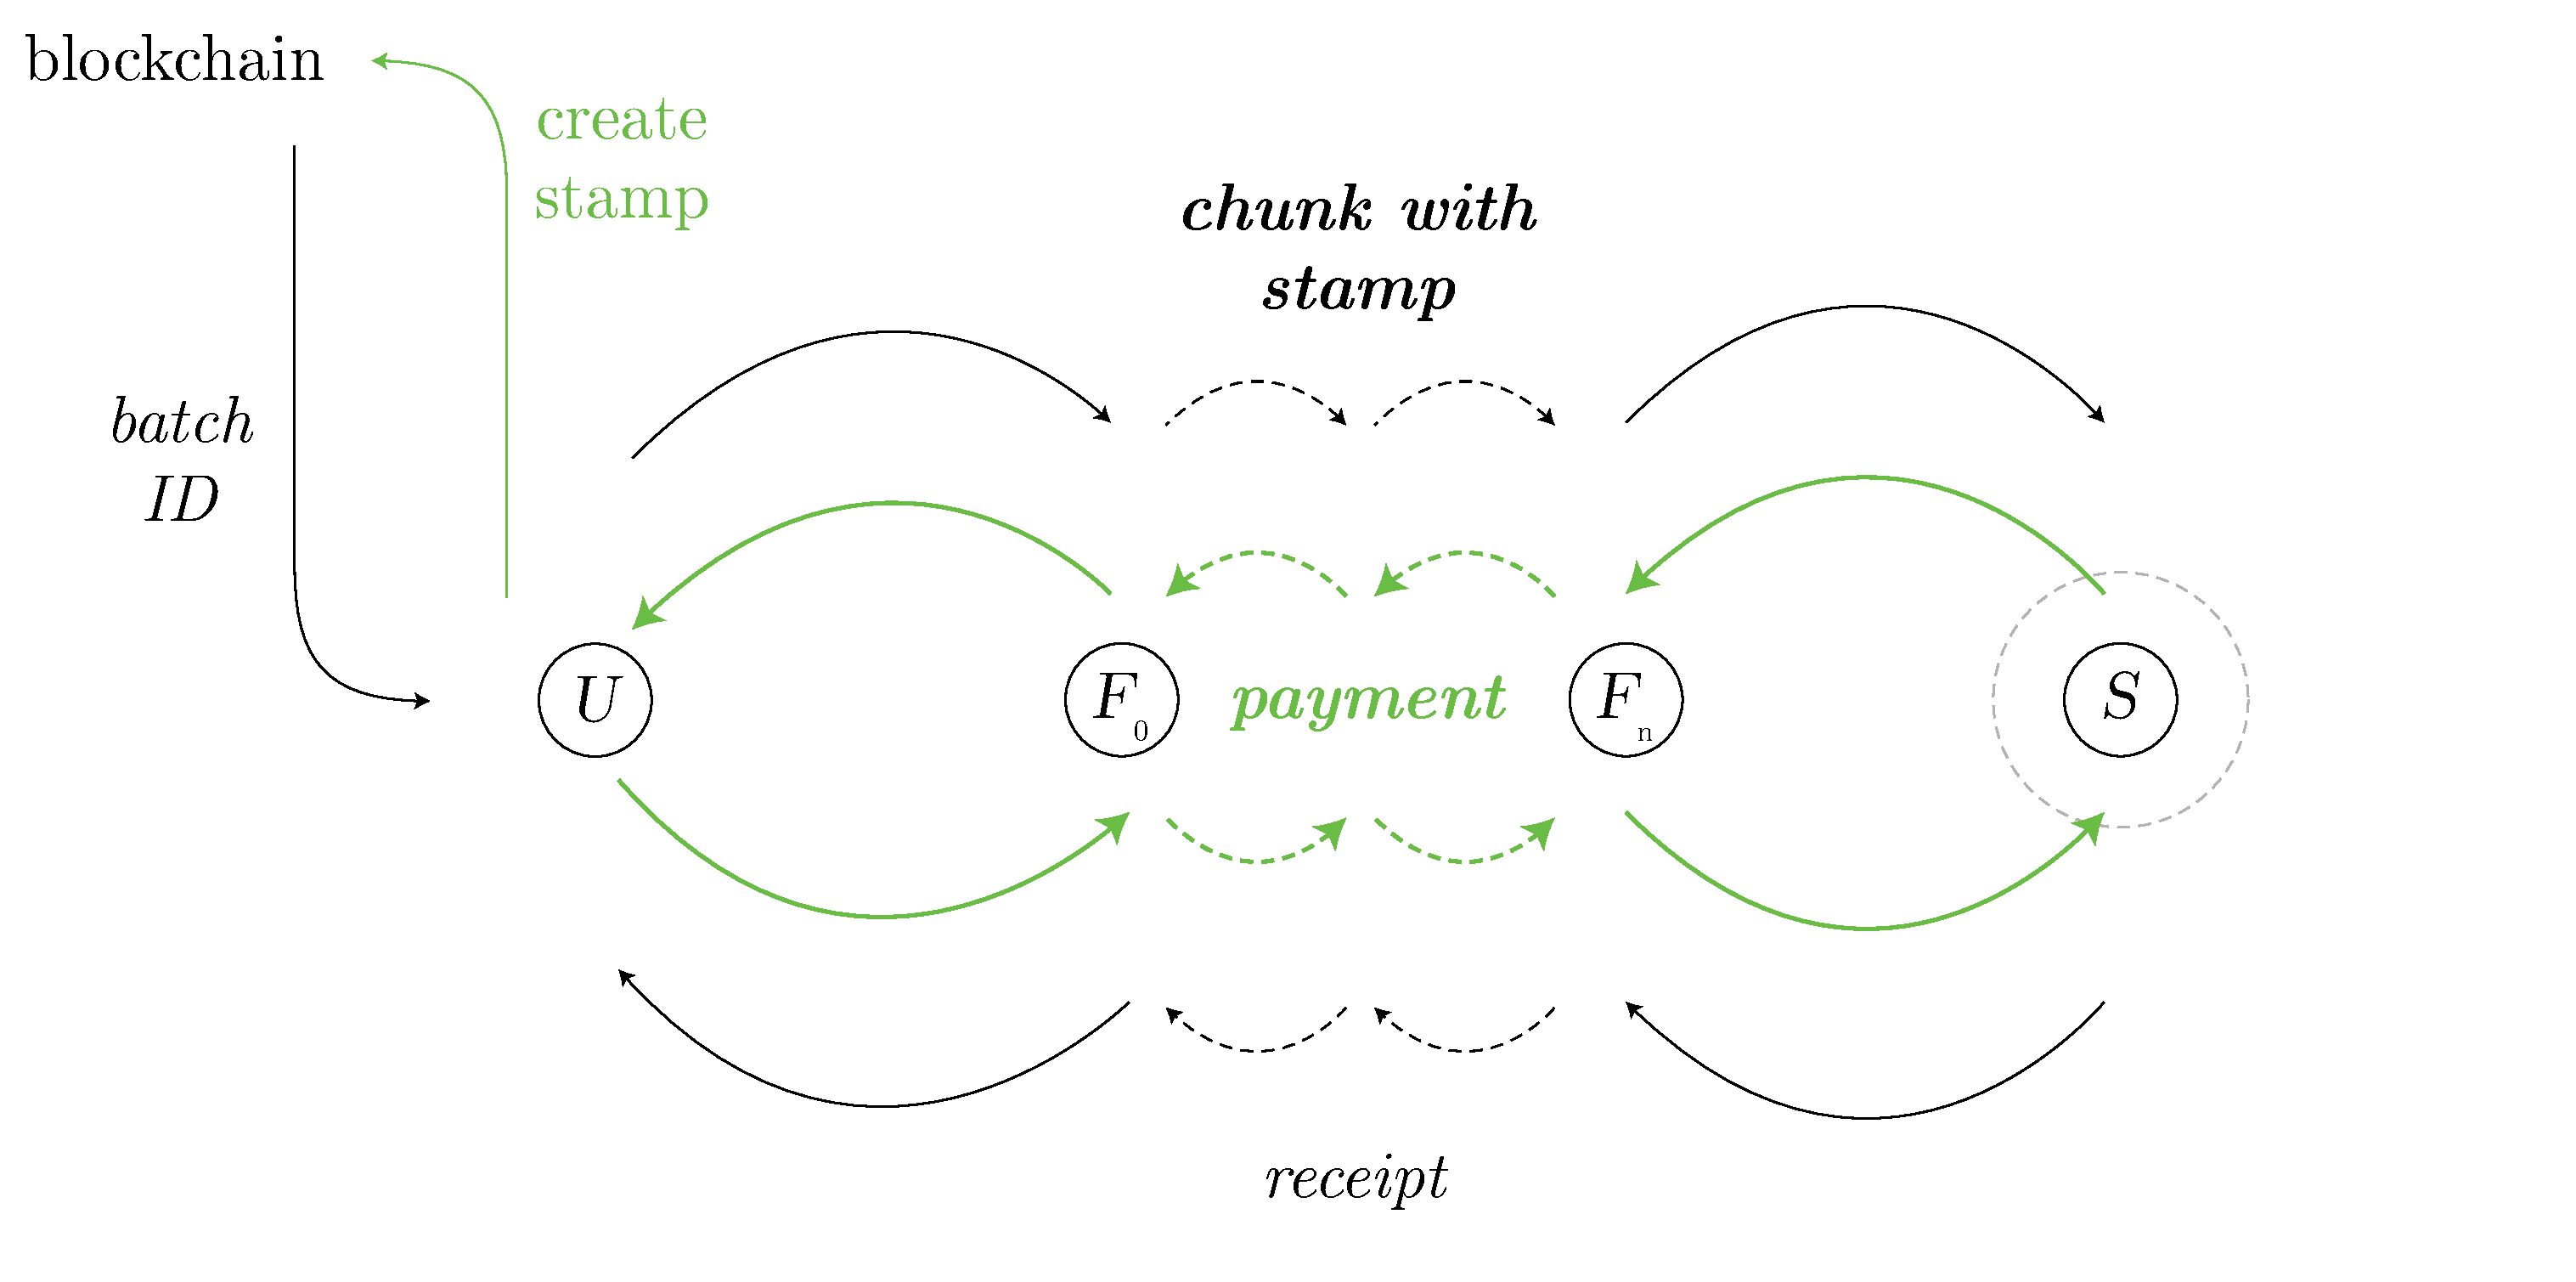
\includegraphics[width=\textwidth]{fig/postage-stamp.pdf}
\caption[Postage stamps  \statusgreen]{Postage stamps}
\label{fig:postage-stamps}
\end{figure}

\subsubsection{Proof of payment}

The proof of payment can lend itself to a number of different implementations. The most obvious choice is to make payments to a central postage stamp issuer smart contract on the blockchain.%
%
\footnote{Using a cheque seems like one option, however, since cheques are signed against cumulative debt and assume the single beneficiary is able to reconstruct the added value over the previously sent cheque. In other words, cheques are not an appropriate means to communicate value to non-peers.}
%
However, because of the high transaction cost, requiring an on-chain payment for each chunk would be prohibitively expensive. Instead, we need a solution that allows the uploader to purchase the postage stamps in a \gloss{postage batch} and then re-use it over many chunks. 


The batches are created by a central postage smart contract when a transaction is sent to its creation endpoint, together with an amount of BZZ tokens and the following transaction data:

\begin{itemize}
\item \emph{owner address} -- The owner that is entitled to use the batches created to stamp chunks.
\item \emph{number of batches} -- Number of batches to be created by this payment.
\item \emph{batch depth} -- Logarithm of the number of chunks that can be stamped with each batch created.
\end{itemize}

This postage payment then results in the following information being recorded:

\begin{itemize}
\item \emph{payment reference ID} -- A random ID that is generated as reference for this payment.
\item \emph{per-chunk balance} -- The total amount, equally allocated for each chunk covered by the batches created from this payment.
\item \emph{owner address} -- The owner that is entitled to use the batches created to stamp chunks.
\item \emph{number of batches} -- The number of batches created by this payment.
\item \emph{batch depth} -- Logarithm of the number of chunks that can be stamped with each batch created.
\end{itemize}


The owner is the address that is specified in the transaction data and recorded as the party authorised to use the batches created to stamp chunks; if not specified, it is assumed to be the transaction sender by default. 

A random identifier is generated to provide a reference to the payment. 
The payment transaction will create multiple batches the number of which is specified in the transaction. The batch depth is eventually recorded for each batch separately. New batches can be created for each payment.
The number of chunks covered by this payment can then be calculated as the sum of the batch sizes. The initial batch depth is meant to apply to all batches created by  the payment transaction. The amount of BZZ tokens sent with the transaction is then allocated equally to all chunks covered by the payment, i.e. the total amount of tokens, divided by the number of chunks covered is assigned to the payment ID to represent the per-chunk balance of the batches. Anyone can then choose to top up this balance at a later date. 


\begin{figure}[htbp]
  \centering
    \includegraphics[width=\textwidth]{fig/postage-stamp-structure.pdf}
  \caption[Postage stamp \statusgreen]{Postage stamp is a data structure comprised of the postage contract batch id, the chunk address and a witness signature attesting to the association of the two. Uploaders and forwarders must attach a valid postage stamp to every chunk uploaded. }
  \label{fig:postage-stamp}
\end{figure}


The postage stamp attached to a chunk is a data structure comprising the following fields (see figure  \ref{fig:postage-stamp}  and the specification in \ref{spec:format:postage-stamps}):

\begin{itemize}
    \item \emph{chunk address} -- The address the stamp is attached to. 
    \item \emph{batch identifier} -- Composed of a payment identifier and a batch index validity of which can be checked with the postage smart contract.
    \item \emph{witness} -- The owner's signature, linking the batch identifier and the owner's address.
\end{itemize}

The \emph{value} of a postage stamp is the per-chunk balance associated with the batch.
Similarly to stamps used for postal mail, a single chunk can have multiple postage stamps attached to it. In this case the value conferred to the chunk by multiple valid postage stamps are added up to form the total postage stamp value. 

\subsubsection{Validity of postage stamp}

A postage stamp's validity can be checked by ensuring the following criteria are met:

\begin{itemize}
\item \emph{authentic} -- The batch identifier is valid, i.e. the payment ID exists and is registered, and the batch index is less than the number of batches associated with the payment ID.
\item \emph{authorised} -- The witness is signed by the address specified as the owner of the batch.
\item \emph{funded} -- The referenced batch has not yet exhausted its balance and is sufficiently funded to cover at least a single storage epoch for the latest  price.
\end{itemize}

All this can be easily checked by the smart contract itself. Validating that less than the total amount of chunks that are allowed to be stamped by a batch are contained within it is crucial. Without further measures, there could be a possibility for an overspend attack in which the uploader reuses the stamp over more chunks than the batch size would warrant and thereby trick the unsuspecting storers into underpaid extra work. 

Protection against such \emph{overissuance} is not trivial: In the absence of global visibility of all chunks signed with a particular batch, nodes cannot directly verify the size, as they have no access to postage stamps attached to chunks that are not relayed through them. Therefore, there needs to be a way for nodes to prevent overissuance collectively, while each must determine how to act based only on locally available information.

\subsubsection{Limiting batch size by constraining prefix collisions}

A solution is to impose an explicit \gloss{uniformity requirement} on the batches: a constraint that chunks signed with the same batch identifier have no \gloss{prefix collision} longer than the depth. A postage stamp with a batch size of $2^d$ can be thought of as a balanced binary tree of depth $d$, where the leaves correspond to maximum length \glossplural{collision slot} of the batch. If the depth of a batch is greater than the depth of the network (log of the number of nodes in the network), then all chunks matching the same collision slot are guaranteed to land in the same neighbourhoods, and, as a result, "violations" of the uniformity requirement can be locally detected by nodes (see figure \ref{fig:prefix-collision}). 
% If storers respond to this violation by randomly keeping only one of the chunks for each collision slot, uploaders will not only lose one chunk if they try to store more then their allowed allocation, but also lose the  predictability of which one on top.
Storer nodes then are expected to  correct the depth recorded with a batch.
They can do the correction by reporting two postage stamps issued by the owner against a batch that are closer than the currently recorded depth for the batch.
The incentive to do this comes from the possibility for a storer to obtain the extra storage cost above the one already paid out.


\begin{figure}[htbp]
  \centering
  \scalebox{0.8}{
\begin{forest}
slot/.style={rectangle,minimum width=9mm, minimum height=9mm},
filled/.style={fill=lightgray},
mid/.style={circle, radius=1mm},
[{},mid,for tree={draw, grow=south}
  [{},mid,edge label={node[midway,left] {0}}
    [{},mid,edge label={node[midway,left] {0}}
      [{},mid,edge label={node[midway,left] {0}}
        [{$0$},slot,edge label={node[midway,left] {0}}]
        [{$1$},slot,edge label={node[midway,right] {1}}]
      ]
      [{},mid,edge label={node[midway,right] {1}}
        [{$2$},slot,edge label={node[midway,left] {0}}]
        [{$3$},slot,edge label={node[midway,right] {1}}]
      ]
    ]
    [{},mid,edge label={node[midway,right] {1}} 
      [{},mid,edge label={node[midway,left] {0}}
        [{$4$},slot,edge label={node[midway,left] {0}}]
        [{$5$},slot,rectangle,filled,edge label={node[midway,right] {1}}
            [{\footnotesize $1010...$},  l=2mm, rectangle, draw=none, edge=dotted]
        ]
      ]
      [{},mid,edge label={node[midway,right] {1}}
        [{$6$},slot,edge label={node[midway,left] {0}}]
        [{$7$},slot,edge label={node[midway,right] {1}}]
      ]
    ] 
  ]
  [{},mid,edge label={node[midway,right] {1}}
    [{},mid, edge label={node[midway,left] {0}}
      [{},mid,edge label={node[midway,left] {0}}
        [{$8$},slot,filled, edge label={node[midway,left] {0}}
            [{\footnotesize $1000...$}, l=2mm, rectangle, draw=none, edge=dotted]
        ]
        [{$9$},slot,edge label={node[midway,right] {1}}]
      ]
      [{},mid,edge label={node[midway,right] {1}}
        [{$10$},slot,edge label={node[midway,left] {0}}]
        [{$11$},slot,edge label={node[midway,right] {1}}]
      ]
    ]
    [{},mid,edge label={node[midway,right] {1}} 
      [{},mid,edge label={node[midway,left] {0}}
        [{$12$},slot,edge label={node[midway,left] {0}}]
        [{$13$},slot,filled,edge label={node[midway,right] {1}}
            [{\footnotesize $1011...$},  l=2mm, rectangle, draw=none, edge=dotted]
        ]
      ]
      [{},mid,edge label={node[midway,right] {1}}
        [{$14$},slot,edge label={node[midway,left] {0}}]
        [{$15$},slot,edge label={node[midway,right] {1}}]
      ]
    ]
  ] 
]
\end{forest}
}  \caption[Limiting the size of a postage stamp \statusgreen]{The postage batch is represented as a binary tree and is maps the stamps issued to the batch.  The leaf nodes are at a level from the root which corresponds to the depth of the postage batch as set at the time of payment. The boxes on the leaf nodes can be thought of as the prefix collision slots. In this figure, the gray boxes represent already filled slots, so the next chunk address should be made to fall into a white one.}
  \label{fig:prefix-collision}
\end{figure}


As chunk addresses are unlikely to be perfectly distributed over the collision slot of a batch, an uploader must keep more than one batch of depth $d$ to sign $2^d$ chunks. In general, the most efficient utilisation of each stamp is by filling all the different \glossplural{collision slot} (see \ref{sec:upload}). Put differently, continued non-uniformity will lead to underutilised stamps, and therefore a higher average unit price for uploading and storing each chunk. This solution has the desired side effect that it imposes an upfront cost to non-uniform uploads: the more focused our upload is on a neighbourhood, the more slots of the postage stamps remain unused. In this way, we ensure that directing too many uploads towards a particular neighbourhood is expensive.%
%
\footnote{The cost of targeted attacks DoS-ing neighbourhoods is exponential with depth.}
%
This will be significant for the later discussion of decentralised file insurance (see \ref{sec:insurance}). 

Another advantage of limiting batch size based on prefix collisions is that with prefix collisions, the absolute value of a postage stamp can be estimated. This comes in handy later when designing the postage lottery (see: \ref{sec:postage-lottery}). 


In order for these collisions to be detectable, the batch size needs to be higher than the estimated neighbourhood depth over the whole lifetime of the batch. In any case, it is not in the interest of users to have batches much deeper than that, since the longer the collision prefixes, the more difficult it becomes to achieve uniformity and fill the entire batch  (see \ref{sec:complexity-filling} of the appendix). 
% We will, for now, just assume that the depth of a batch is a fixed number set centrally in the contract and that follows the depth of Swarm. The effect of network growth on the already used stamps is discussed below.


\subsubsection{Mining chunks using encryption}

One neat solution to completely fill up \glossplural{postage batch} relies on the insight hinted at in \ref{sec:chunk-encryption}: Choosing the encryption key allows us to \emph{mine} a chunk to a specific postage batch.

The process of finding an encryption key to generate a content hash close to an address is analogous to mining blocks in a blockchain. Encryption of chunks requires a 32-byte key, which plays the role of the nonce in a block, that is: It provides enough entropy to guarantee that one is able to find an encryption key such that the hash digest of the resulting encrypted chunk produce an address which falls into a particular slot within an open postage batch. The difficulty of mining is determined by the batch depth. 

Consider the thrifty uploader that only has as many postage collision slots as chunks to send. Given a postage batch with depth $d$, they encrypt the chunk with a key chosen such that the resulting encrypted chunk's address fills a free collision slot of an open postage batch. As shown in the analysis found in appendix  (\ref{sec:complexity-filling}), this strategy of filling a batch requires an average of $0.69d+1$ trials per chunk, i.e. 8, 15, 22 for a thousand, million and billion nodes respectively. This is found to be of a reasonable complexity.


\subsection{Postage lottery: positive incentives for storage \statusyellow}\label{sec:postage-lottery}

\yellow{}

As discussed in \ref{sec:accounting}, the primary incentive mechanism in Swarm is providing compensation for retrieval, where nodes are rewarded for successfully having served a chunk. This reward mechanism has the added benefit of encouraging opportunistic caching. Profit-maximising storage nodes serve chunks that are often requested from them and as a result, ensure that popular content becomes widely distributed across the network and thus also the retrieval latency is decreased.

The flipside of using only this incentive, is that chunks that are rarely retrieved may end up being lost: If a chunk is not being accessed for a long time, then as a result of limited storage capacity, it will eventually end up garbage collected to make room for new arrivals. In order for the swarm to guarantee long-term availability of data, the incentive system needs to make sure that additional revenue is generated for chunks that would otherwise be deleted. In other words, unpopular chunks that do not generate sufficient profit from retrievals should compensate the nodes that store them for their opportunities forgone. The \gloss{postage lottery} presented in this section provides such a compensation through redistributing the revenue coming from postage stamps among the storer nodes in a fair way.



Central to the postage lottery scheme is the realisation that probabilistic payments can be used to create revenue for storer nodes.
Using a lottery allows us to calibrate earnings that in the long run will have the same payout as if there was an actual payment for each chunk, yet save on transaction costs and provides the randomness which is necessary to serve as spot-checks.


\subsubsection{Race: raffle, apply, claim and earn}

The postage lottery takes place on an \gloss{EVM} blockchain and is managed by a smart contract. The lottery process is defined by the following protocol (see formally in \ref{spec:format:postage-stamps}). 

Every $N$-th%
%
\footnote{$N$ is chosen so that the period  between two rounds comfortably accommodates all phases of the lottery process.}
%
block on the blockchain marks the beginning of a new global lottery round.
The subsequent $N$ blocks are composed of three phases representing periods during which the participants in the raffle are expected to send transactions to interact with the raffle smart contracts: 

\begin{enumerate}
\item \emph{pre-committal} -- nodes pre-commit to the raffle challenge by sending in a price offer. As a result of valid pre-committal transactions, a set of applicants is defined. The end of this period is marked by the selection of the witness batches.
\item \emph{submission} -- nodes send a list of chunks and their proofs of custody as dictated by the witness batches. As a result of valid claim transactions, a set of claimants are defined. The end of this period is marked by the selection of challenges.
\item \emph{refutation} -- nodes send refutations of the challenges. As a result of valid refutations, a set of final prize winning claimants are determined. The end of this period is marked by the payout to the winners.
\end{enumerate}

The moment the last period ends a new raffle round begins. The lottery and its phases can also be characterised by the acronym \gloss{race}, with, of course, an mnemonic resolution detailing the phases: \gloss{raffle--apply--claim--earn}. The timeline of events is depicted in figure \ref{fig:raffle-timeline}.


\subsubsection{Automatic raffle rounds}

The RACE process is initialised with the raffle phase. First, the hash of the starting block is hashed together with integers from $0$ up to $n-1$ to obtain $n$ \emph{winning tickets} ($r_0, \ldots r_{n-1}$) each of which represents an independent \gloss{raffle draw}.%
%
\footnote{Multiple raffles each round are needed to calibrate the expected frequency for a node to win a raffle. By increasing $n$ as the network grows the expected time needed to get compensated for storage services can be kept constant.}. 
%
Once these winning tickets have been produced, nodes whose addresses are in the close proximity of the ticket $r_i$ are then able to apply to participate in the applicable raffle.


From the network perspective, these raffles serve as spot checks on storer nodes, whereas from the storer nodes' perspective, raffles represent the means of securing compensation for providing network storage within the swarm. 


\begin{figure}[htbp]
  \centering
  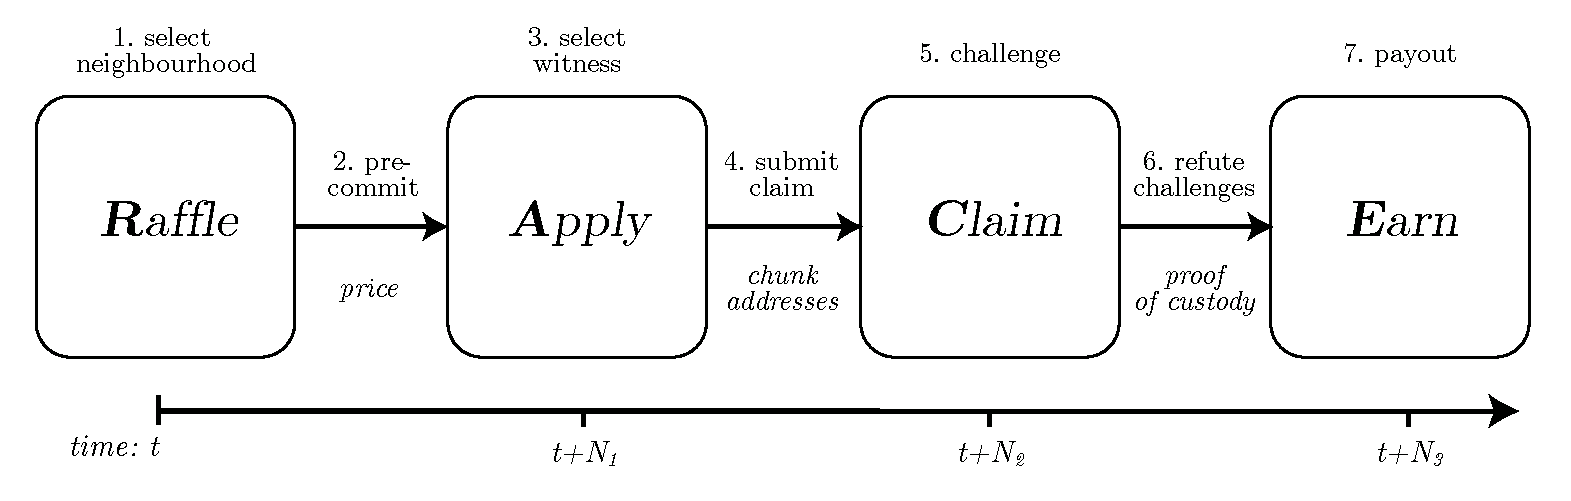
\includegraphics[width=\textwidth]{fig/postage_race.pdf}
  \caption[Timeline of events in a raffle round \statusgreen]{Timeline of events in a raffle round.}
  \label{fig:raffle-timeline}
\end{figure}


\subsubsection{Apply: precommit to raffle challenge}

In the first interactive phase, in order to apply for the prize, all nodes in the proximity of the winning ticket must send a transaction to the lottery contract including a price offer for storing a chunk per block. By submitting such a price, a node implicitly declares that it has in its possession all chunks of all batches with value higher than the price within their radius of responsibility. This radius of responsibility is self-claimed by the nodes and is part of the pre-committal. 

% \begin{figure}[htbp]
%   \centering
%   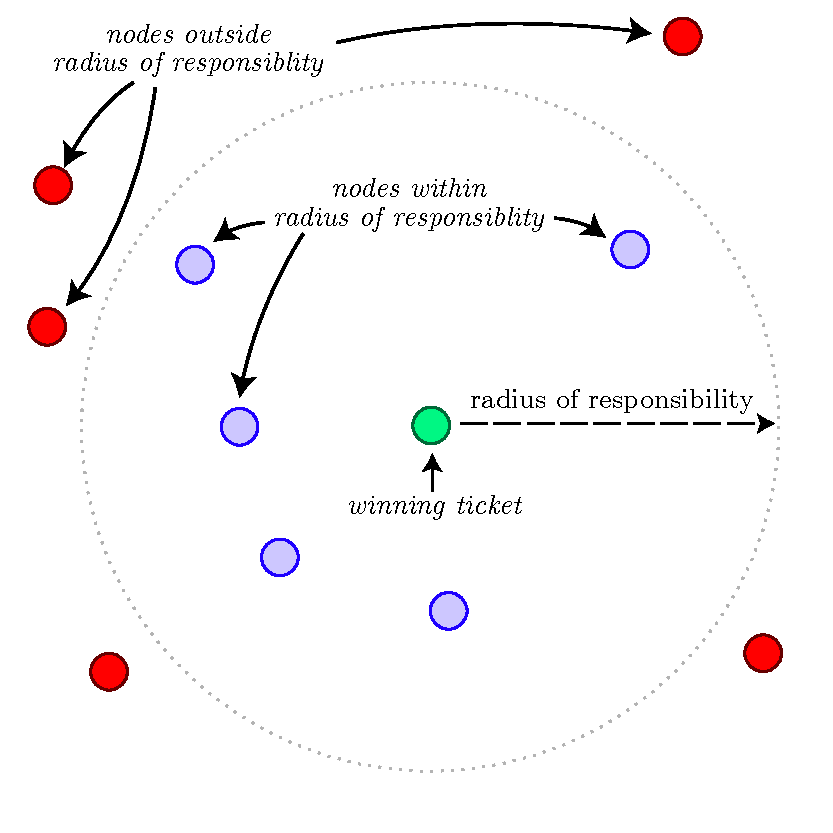
\includegraphics[width=.7\textwidth]{fig/radius_of_responsibility.pdf}
%   \caption[Radius of responsibility for postage lottery claims \statusorange]{Radius of responsibility for postage lottery claims}
%   \label{fig:raffle-radius}
% \end{figure}

\subsubsection{Claim: submit proofs to win}

After this application deadline has passed, the raffle enters into the claim phase by designating a \gloss{witness batch} for each applicant. This witness batch serves as a spot check for the applicant's claim that they store all the chunks that they are responsible for. Analogous to the winning tickets, the witness batch is selected based on randomness provided by the \gloss{blockhash} of the block that closes the application round $h_1$.  The spot check is implemented  by the following procedure. First create an anchor by hashing together the blockhash $h_1$ and the applicant's address, and then choose the batch which has the id closest to the anchor and has a value above the price submitted in the application. This batch serves as the random witness batch against which applicants will submit evidence that they are still in custody of all their allocated chunks. 

As we have discussed previously, stamps attached to a chunk endow that chunk with a value, as defined by the per-chunk balance of the batch. Pursuing a \gloss{value-consistent garbage collection strategy} (see \ref{spec:strategy:garbage-collection}) implies that the minimum postage stamp value accepted on a chunk will coincide with the storer node's garbage collection cutoff value. Nodes that follow this strategy faithfully, know that they have never deleted a chunk whose postage value was above their minimum required postage value. In this way, they can be confident that they are able to include all relevant chunks above that value, no matter which batch is selected to be the witness.

The claim phase is separated from the application phase exactly in order to force applicants to pre-commit to any spot check, since: if the witness was known at the time of application, frivolous nodes could simply claim the prize even if they just serendipitously stored only the chunks of the witness batch.  In  order to discourage such     opportunistic   behaviour, participation in the raffle requires a deposit sent  with the precommittal. This amount is added to the reward pool if the node fails to survive the remaining phases of  the raffle round, otherwise given back to the applicant.

To claim the raffle prize, a node must show that they have every witness chunk, i.e. every chunk stamped with the witness batch that falls within their radius of responsibility. In order to prove possession of chunk data, nodes must submit a \gloss{batch proof of custody}, a canonically ordered list of \glossplural{BMT proof} (see \ref{spec:format:bmt}), one for each witness chunk (see figure 
\ref{fig:batch-proof-of-custody}). Applicants have $N_2$ blocks to submit their claim, after which the raffle enters the challenge phase. Applicants that applied but failed to submit a claim are treated as if they had submitted an invalid claim.   


\begin{figure}[htbp]
  \centering
   \includegraphics[width=\textwidth]{fig/batch-proof-of-custody.pdf}
  \caption[Batch proof of custody \statusgreen]{Batch proof of custody. A Proof of custody is BMT inclusion proof wrapped with the chunk address, the segment index and the postage stamp. Multiple POCs are packaged with a witness batch id.}
  \label{fig:batch-proof-of-custody}
\end{figure}

\subsubsection{Earn: challenging the applicants}

% If the set of chunks presented to the blockchain is incomplete (i.e. it doesn't contain all chunks for which a statement of custody receipt was issued), the applicants can be challenged on the blockchain. The challenge contains a statement of custody receipt that was signed previously by the applicant (see \ref{sec:push-syncing} and \ref{sec:push-sync-incentives}). This receipt can then be submitted by any third party and is validated right away by the smart contract. If the challenge is valid, the applicant loses their registration immediately and more punitive measures may be enacted by his peers. Challengers have till the end of the raffle round to challenge applicants.

\subsubsection{Choosing the winner}

After the challenge phase ended ($N$ blocks after the beginning of the raffle round), from amongst the applicants that have survived the challenge period, for each raffle, the ones that offered the lowest prices will win the round. The  price itself is the lowest price that any of the neighbourhood's winners applied with.

The lottery prize payout needs to take into account the number of winners, the number of chunks, the proportion of a nodes' storage with respect to the total volume stored in Swarm.
The period that the payout is for is equally distributed among winners. For ease of reasoning, it is possible to calibrate blocks = winners, so that we can say a node when it wins gets paid for all chunks for a block. The winner is entitled to collect the price for each chunk whose price is not lower than the minimum required by the winner. The sum of all winners' proceeds is subtracted from the remaining balance of each batch. The postage batches whose balance is dried out after the payout are removed from the contract.%
%
\footnote{In practice, such a balance adjusment is unnecessary, see \ref{spec:format:postage-stamps}).
}

While winning nodes could try to benefit from a higher price for a bigger win, they are competing with each other to try to win the raffle, so they are incentivised to secure their win by offering the actual cutoff value they used for garbage collection. As a result of competitive payouts, it is expected that the unit prices will converge on the marginal cost of storing one more chunk.




\subsubsection{Batch depth and volume adjusted payouts}

So far, for ease of reasoning, we assumed that the depth of each batch was given.  The requirements of batch depth are that it is deeper than the neighbourhood depth so that prefix collisions are always caught by storer nodes, yet not too much deeper so that it would make batches too difficult to fill completely (see \ref{sec:complexity-filling}). If a batch of depth $b$ has been filled completely, then a storer node with radius of responsibility $d$ is expected to store  $2^{b-d}$ chunks belonging to this batch.
Half of these with proximity of order $d$ to the winner's address. 

In order to incentivise $r$ redundant replicas of chunks, each stored at one of  the  nodes in a neighbourhood, winners are expected to store the same chunks. 
Moreover, partial storage of a batch's chunks should be discouraged. 
Both are  taken care of if nodes are incentivised to present the most chunks they possibly can for a batch.
This incentive translates to partial  storage of local chunks of a match leads to lower winnings. This is achieved if each batch detected depth as well as actual size are both reported as part of the precommit. Falsely committing to more chunks than stored by the node for a batch runs the risk of an unrefutable challenge on the batch (if designated as a witness) resulting in losing the price one-time raffle ticket on top of not earning  the raffle prizepool. All this aligns uploaders   and storers on attempting to use completely filled batc hes (the collision slots constituting a balanced binary tree of depth $b$.)
Since the actual sizes constitute an estimation of actual chunk volume is swarm. 

The best arrangement of storer is if the 
In particular we propose that a volume-adjustment scheme is used  when applicants 

This is implicit in the require
Conversely, based on the actual number of chunks per batch presented to the contract by winners, $C$ we can make an estimate of the current neighbourhood depth in Swarm as $d'\defeq b - \mathit{log}_2(C)$. This gives the chance for the lottery smart contract to serve as a depth oracle. The oracle value can also be used as the minimum depth for any postage batch in the raffle calculations. Note that if self-claimed depth of a batch can be lower than the typical neighbourhood depth, then nodes are expected to have at  most one chunk of a batch in their storage and therefore unable to report overissued batches. Therefore active batches has the minimum size of $2^{d+1}$.


Practically old completely filled postage batches can either be retained or the content they cover can be re-insured. In the former case, a node would want to retain the batch in case the network wide neighbourhood depth grows and exceeds the original depth of the batch, in which case the owner is able to add chunks to it legitimately. 
In order to add new chunks to a batch without collisions, one must remember the chunks they have already associated with the batch.%
%
\footnote{In fact is actually sufficient to just remember which collision slots were filled up to a depth that could possibly be reached by the growing network. In practice, as an optimisation, potential collision slots for depth  $b' >b$ can be recorded using a bit vector of length $2^{b'-1}$}
%

Note that owners can choose to pay an amount for postage that, even if the swarm grows a thousand fold, the balance would run dry only after a desired period. This becomes important in the context of \gloss{upload and disappear}.
Such deep batches require the same $O(\mathit{log}(n))$ computational overhead (see \ref{sec:complexity-filling}). This essentially means a discount   requiring  bulk purchase/use.





% \subsubsection{Statement of custody receipts}

% Statement of custody receipts are crucial in the lottery, as they enable nodes to challenge. The challenge constitutes of submitting a receipt signed by the applicant. It is either a chunk closest to the applicant or to one of its neighbours. If the challenge is valid, the applicant loses their registered status. 

% In order for syncing neighbours to be able to challenge, nodes need to attach a statement of custody receipt to all the chunks that they are closest to or that their neighbour peer is closest to. The peers can be sanctioned with disconnection and blacklisting in case of non-compliance. 

% As part of syncing, an aspiring storer node must sign statements of custody receipts for all the chunks that it is closest to. If the upstream peer did not require these, then they could not defend their territory as it were, i.e. they would have no grounds to challenge the new node when they apply for winning a raffle round after registering. Note that they do not need to keep all of the chunks, since one is enough to mount a challenge. Additionally, the upstream node is not incentivised to withhold chunks that belong to the new node as they cannot earn any lottery winnings from them once the new node enters the race. 

\subsubsection{Incentives implicit in the lottery}

This procedure incentivises nodes to adhere to the following behaviors:

\begin{itemize}
\item \emph{stay online} -- Otherwise the raffle is missed.
\item \emph{have a redundantly synced area of responsibility} -- Remain fully synced with their neighbourhood. Otherwise the claim may be incomplete and the volume-adjustment leaves the node with less.
\item \emph{have a fully indexed local store} -- To be able to list all chunks of a batch, nodes need to preserve postage stamps and keep an associated set of chunk addresses. 
\item \emph{perform value consistent garbage collection} -- In order to tell if the node locally stores all previously receipted chunks of a batch they must perform garbage collection value-consistently,%
%
\footnote{or store indexes of deleted chunks which is inefficient}
i.e. the minimum value accepted coincides with the maximum value ever deleted.
%
\item \emph{store the data} -- In order to provide BMT proofs the node must possess the data in the chunk content.%
%
\footnote{In the special case of addressed envelopes with pre-paid postage, no payout can be collected before the envelope has been filled and sent (see \ref{sec:addressed-envelopes}).}
\end{itemize}


\subsection{Price signalling capacity pressure \statusyellow}\label{sec:capacity-pressure}

\yellow{}

\subsubsection{Storage capacity}
Kademlia topology and the redundancy parameter determine the node's neighbourhood depth (see \ref{sec:redundancy-by-local-replication}). The neighbourhood depth delineates the area of responsibility. As a result of postage lottery, the nodes are incentivised to have a uniform neighbourhood size. The number of chunks uploaded to that area is simply proportional to the number of all chunks uploaded to Swarm $C$ and inversely proportional to the number of nodes in Swarm $N$. The number of chunks stored by a node is on average $CR/N$, where $R$ is the neighbourhood replication factor, measuring the degree of redundancy. This expresses the density of chunks in any neighbourhood. Given a particular connectivity and fixed storage quantity for a neighbourhood, $C/N$ captures the \emph{storage capacity pressure}. 

If we assume that chunks are meant to be preserved only for a limited period of time, then within some variance the pressure stays constant. In other words, we can find a network size%
%
\footnote{in the sense of storage capacity; or in the sense of number of nodes assuming a minimum storage capacity per node.}
%
such that all content that users want preserved is preserved. 

If the rate of new uploads to Swarm is higher than the rate of expiry (postage stamp balances going below the current price), then a fixed network will experience increasing pressure. As a consequence, without added capacity, after a while, content that is meant to be preserved will be garbage collected. 

Such capacity shortage is solved if added storage is invited by incentivising new storer nodes to join the network or rising demand is resisted by raising prices. Conversely, if the rate of expiry is faster than new uploads, pressure decreases and there may well be surplus capacity. The resulting situation with underutilised resources is remedied if added content is invited by incentivising users to upload their content or by some nodes dropping out disincentivised by lower prices. Thinking in terms of supply and demand, we can reach a self-regulating market simply if storage capacity pressure is signalled in the price of storage, i.e. the minimum value for postage stamp per chunk. 

\subsubsection{Garbage collection strategy and postage value}

The emergence of this self-regulating market is exactly what happens if we ensure that the garbage collection queue is prioritised by descending postage value (see \ref{spec:strategy:garbage-collection}).

\begin{figure}[htbp]
  \centering
  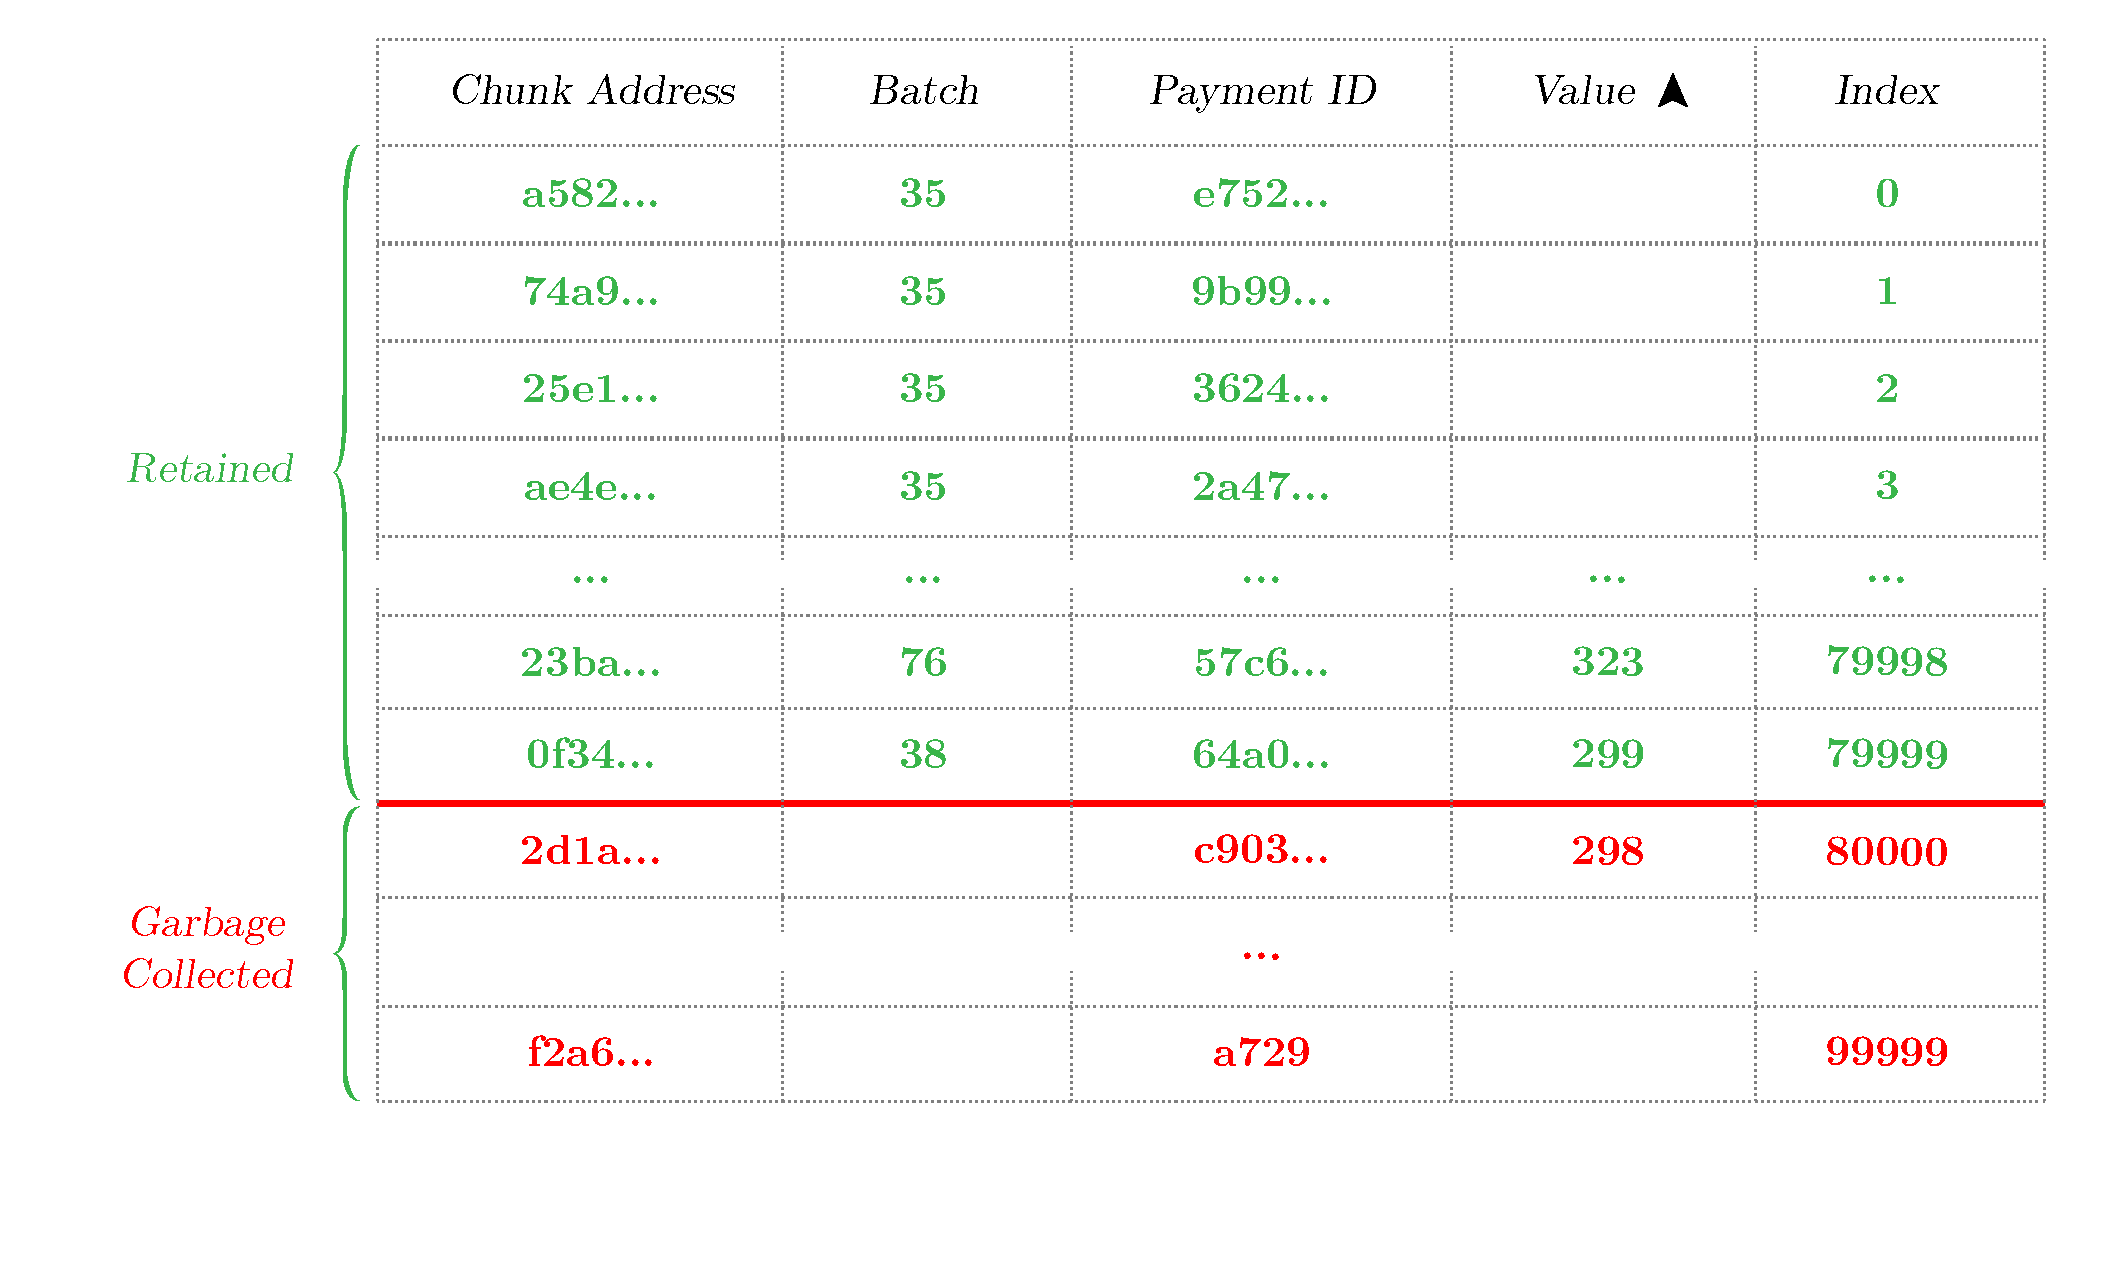
\includegraphics[width=\textwidth]{fig/garbage-collection-fixed.pdf}
  \caption[Garbage collection \statusgreen]{Garbage collection: chunks are ordered by profitability which comes from the postage value and a predicted retrieval revenue.}
  \label{fig:garbage-collection}
\end{figure}


Note that when a raffle round pays out, the same amounts get subtracted from all stamp balances. Therefore, the ordering by value does not change no matter how many raffle rounds have happened. However, in order to insert a newly created postage stamp, we will need to know the overall amount paid out so far and then add it to the new item's value.

A postage stamp must promise sufficient earnings with its value for the storer so that it outperforms the lowest quantile of competitors. When a node appends chunks to the bottom of the garbage collection queue, the postage value is updated by checking if there was a top-up on the blockchain.%
%
\footnote{In order to avoid checking updates on the blockchain for payout rate change, a node may just want to update the rate as a response to a payment event logged on the lottery contract.}
%
If there was a change, the chunk will need to be reinserted in the queue. 

\subsubsection{Combining retrieval popularity and postage value}

Besides expected lottery payouts, estimation of profitability needs to factor in earnings from serving popular chunks. If we record the number of times a chunk is served for every raffle \gloss{epoch}, then one can apply a predictive model to these datapoints to forecast the earnings for a future period. Fortunately, we only really need to decide which are the least profitable chunks. 

% The distribution of popularity is a power law distribution with a long  tail. Unless Swarm's capacity is so constrained that only popular chunks can be stored, we expect that nearly  half of chunks will not be accessed at all.


When we iterate over the chunks with the smallest postage value, we must decide if each chunk should survive the next epoch or if it has no real promise of being requested. The garbage collection process will then terminates once number of chunks matching the volume of a quantile have been deleted (see figure \ref{fig:garbage-collection}).

\subsubsection{Uniformity of prices} 

When push-syncing chunks, each forwarding node accepts chunks only if their postage value is higher than that node's advertised minimum. Practically this means that the initial postage value cannot be lower than the maximum such value in the network, otherwise syncing is not successful. This means that nodes keeping their postage price offer for the lottery low will not receive more traffic, they just have more chance of winning and need to have more storage capacity than their more expensive neighbours to be able to store the extra chunks whose value reached below their neighbour's minimum.

If neighbourhoods manage to keep their prices high, it will attract new nodes who will under-offer. If the high prices were genuine due to actual capacity shortage, then the new node adds storage space and corrects the non-uniformity. If the neighbourhood kept high prices because they cartellised, then the new node is able to disrupt this. Over a longer time period, therefore, prices are expected to converge.



% Whenever we serve a chunk we update the value of the chunk by adding the retrieval price. For the sake of simplicity, let us assume that there is the garbage collection cycle and the raffle round is at the same time. Knowing the earnings of the last epoch, we recalibrate the chunk profitability predictive model. 





\subsection{Insurance: negative incentives \statusorange}\label{sec:chunk-insurance}

\orange{taken from earlier paper mostly - to be rewritten much shorter to reflect latest}

The storage incentives presented so far refer to the ability of a system to encourage the preservation of content through monetary rewards given to storers. This was achieved using a postage lottery which instrumented the fair redistribution of postage payments to storers. With this scheme, we provided positive incentivisation on a collective level. Such a system,  however, is suspect to the \gloss{tragedy of the commons} problem in that disappearing content will have no negative consequence to any one storer node. The lack of individual accountability renders the storage incentivisation limited as a security measure against data loss. Introducing competitive insurance, on the other hand, adds an additional layer of negative incentives and forces storers to be very precise with their commitments to provide users with reliability. Particular attention is required in the design of the incentive system to make sure that failure to store every last bit promised is not only unprofitable but outright catastrophic to the insurer. 

\subsubsection{Punitive measures}

Unlike in the case of bandwidth incentives where retrievals are immediately accounted and settled, long-term storage guarantees are promissory in nature and it can only be decided if the promise has been kept at the end of its validity. Loss of reputation is not sufficient as a deterrent against foul play in these instances: since new nodes must be allowed to provide services right away, cheaters could just resort to new identities and keep selling (empty) storage promises.

We need the threat of punitive measures to ensure compliance with storage promises. These will work using a \emph{deposit system}. Nodes wanting to sell promissory storage receipts should have a stake verified and locked-in at the time of making their promise. This implies that nodes must be registered in advance with a contract and be made to put up a \gloss{security deposit}. Following registration, a node may sell storage promises covering the time period for which their funds are locked. While their registration is active, if they are found to have lost a chunk that was covered by their promise, they stand to lose their deposit.

\subsubsection{Requirements}

Let us start from some reasonable guiding principles:

\begin{itemize}
\item Owners need to express their risk preference when submitting to storage.
\item Storers need to express their risk preference when committing to storage.
\item There needs to be a reasonable market mechanism to match demand and supply.
\item There needs to be guarantees for the owner that its content is securely stored.
\item There needs to be a litigation system where storers can be charged for not keeping their promise.
\end{itemize}

Owners' risk preference consist of the time period covered as well as a preference for the \emph{degrees of reliability}. These preferences should be specified on a per-chunk basis and they should be completely flexible at the protocol level.

Satisfying storers' risk preferences means that they have ways to express their certainty of preserving what they store and factor that in their pricing. Some nodes may not wish to provide storage guarantees that are too long term while others cannot afford to stake too big of a deposit. This differentiates nodes in their competition for service provision.

A \emph{market mechanism} means there is flexible \emph{price negotiation} or discovery or automatic feedback loops that tend to respond to changes in supply and demand.

In what follows we will elaborate on a class of incentive schemes we call \gloss{swap}, \gloss{swear} and \gloss{swindle} due to the basic components:

\begin{itemize}
\item [\emph{swap}]
  Nodes are in quasi-permanent long term contact with their registered peers. Along these connections the peers are swapping chunks and receipts triggering swap accounting (see \ref{sec:accounting}).
  
\item [\emph{swear}]
  Nodes registered on the Swarm network are accountable and stand to lose their deposit if they are found to violate the rules of the Swarm in an on-chain \gloss{litigation} process.

\item [\emph{swindle}]
  Nodes monitor other nodes to check if they comply with their promise by submitting challenges according to a process of litigation.

\end{itemize}

\subsubsection{Contracts through receipts}

A \gloss{litigation} procedure necessitates that there are contractual agreements between parties ultimately linking an owner who pays for securing future availability of content and a storer who gets rewarded for preserving it and making it immediately accessible at any point in the future. The incentive structure needs to make sure that litigation is a last resort option.

The simplest solution to manage storage deals is to use direct contracts between owner and storer. This can be implemented by ensuring storers return signed receipts of chunks they accept to store and owners pay for the receipts either directly or via escrow. In the latter case, the storer is only awarded the locked funds if they are able to provide proof of storage. This procedure is analogous to the postage stamp lottery process. Insurance can be bought in the form of specially marked postage stamps, statements of custody receipts can close the loop and represent a contract between uploader and storer. Outpayments conditional on proofs of custody can be implemented the same way as the lottery.

Failure to deliver the stored content is penalised even when the consumer who tried to access the chunk but was unable, was not party to the agreement to store and provide the requested content. Litigation is therefore expected to be available to third parties wishing to retrieve content.

If the pairing of chunks and receipts is public and accessible, then consumers/downloaders (not only creators/uploaders) of content are able to litigate in case a chunk is found to be missing (see \ref{sec:insurance}). 

\subsubsection{Registration}

Before a node can sell promises of long-term storage, it must first register via a contract on the blockchain we call the \gloss{SWEAR} contract. The SWEAR contract allows nodes to register their public key to become accountable participants in the Swarm. Registration is done by sending the deposit to the SWEAR contract, which serves as collateral in case the terms that registered nodes "swear" to keep are violated (i.e. nodes do not keep their promise to store). The \emph{registration} is valid only for a set period, at the end of which a Swarm node is entitled to their deposit. Users of Swarm should be able to count on the loss of deposit as a disincentive against foul play for as long as enrolled status is granted. Because of this the deposit must not be refunded before the registration expires. The expiry of the insurance period should therefore include a final period during which the node is not allowed to issue new receipts but can still be challenged.

When a registered insurer node receives a request to store a chunk that is closest to them, it can acknowledge it with a signed receipt. It is these signed receipts that are used to enforce penalties for loss of content. Because of the locked collateral backing them, the receipts can be viewed as secured promises for storing and serving a particular chunk.



\subsubsection{Submitting a challenge}


If a node fails to observe the rules of the Swarm they swear to keep, the punitive measures need to be enforced which is necessarily preceded by a litigation procedure. The implementation of this process is called \gloss{SWINDLE}.

When a user attempts to retrieve insured content and fails to find a chunk, they can report the loss by submitting a \gloss{challenge}. This scenario is the typical context for starting \gloss{litigation}. This is analogous to a court case in which the issuers of the receipts are the defendants who are guilty until proven innocent. Similarly to a court procedure, public litigation on the blockchain should be a last resort when the rules have been abused despite the deterrents and positive incentives.


The challenge takes the form of a transaction sent to the SWINDLE contract in which the challenger presents the receipt(s) for the lost chunk. Any node is allowed to send a challenge for a chunk as long as they have a valid receipt for it (although it may not have necessarily been issued to them). The same transaction also sends a deposit covering the price of the upload of a chunk. The validity of the challenge as well as its refutation need to be easily verifiable by the contract.
The contract verifies if the receipt is valid, i.e. 1) authentic, 2) active and 3) funded, by checking the following conditions:

\begin{itemize}
\item \emph{authentic} -- The receipt was signed with the public key of a registered node.
\item \emph{active} -- The expiry date of the receipt has not passed.
\item \emph{funded} -- Sufficient funds are sent alongside it to compensate the peer for uploading the chunk in case of a refuted challenge.
\end{itemize}

The last point above is designed to disincentivise frivolous litigation, i.e. bombarding the blockchain with bogus challenges and potentially causing a DoS attack.

The contract comes with an accessor for checking that a given node is challenged (potentially liable for penalty), so the challenged nodes can be notified that they must present the chunk in a timely fashion. The challenge is then kept open for a fixed amount of time, the end of which essentially is the deadline to refute the challenge. 

\wip{still pondered - fingerpointing is not necessary}

\subsubsection{Fingerpointing or proof of storage}


The node implicated can refute the challenge by sending a transaction to the blockchain with either the direct refutation (a proof of custody or the chunk itself depending on the size) or a receipt for the same chunk signed by another node. This receipt needs to be issued by a nearer neighbour (a registered peer closer to the chunk address than the node itself). In other words, if a node is accused with a receipt, they can  shift the blame and provide a valid receipt from a nearer neighbour.%
%
\footnote{The contract can easily verify if the newly challenged node (the one that signed the receipt submitted as a refutation) is closer to the chunk address than the originally challenged node.}
%
Thus litigation can trigger a chain of challenges with receipts pointing from the initially challenged node all the way to a node that can shift the blame no further and therefore must present the chunk or be punished. This way of refuting a challenge is called \gloss{fingerpointing}. 

Upon verifying the format of the refutation, the contract checks its validity by checking the hash of the chunk payload against the hash that is litigated or validating the proof of custody. 

If a challenge is refuted within the period the challenge is open, the deposit of the accused node remains untouched. The cost of uploading the chunk must be reimbursed to the uploader from the deposit of the challenge, but in order to prevent DoS attacks, this deposit should actually be substantially higher than this in any case (e.g. a small integer multiple of the corresponding gas price). After successful refutation the challenge is cleared from the blockchain state.

This challenge scheme is the simplest way (1) for the defendants to refute the challenge as well as (2) to make the actual data available for the nodes that needs it.

\subsubsection{Successful challenge and enforcement}

If the deadline passes without successful refutation of the challenge, then the charge is regarded as proven and the case enters into the enforcement stage. Nodes that are proven guilty of losing a chunk lose their deposit. Enforcement is guaranteed to be successful by the fact that deposits are kept locked up in the SWEAR contract.

If, on litigation, it turns out that a chunk (that was covered by a receipt) was lost, the deposit must be at least partly \emph{burned}. Note that this is necessary because, if penalties were paid out as compensation to holders of receipts of lost chunks, it would provide an avenue of early exit for a registered node by "losing" bogus chunks that had been deposited by colluding users. Since users of Swarm are interested in their information being reliably stored, their primary incentive for keeping the receipts is to keep the swarm motivated to do so, not the potential for compensation in the case they do not. If deposits are substantial, we can get away with paying out compensation for initiating litigation, however we must have the majority (say 95\%) of the deposit burned in order to make sure this easy exit route remains closed.

Punishment can entail \emph{suspension}, meaning a node found guilty is no longer considered a registered Swarm node. Such a node is only able to resume selling storage receipts once they create a new identity and put up a deposit once again. Note that the stored chunks are in the proximity of the address, so having to create a new identity will also imply expending extra bandwidth to replenish storage. This is an extra pain inflicted on offending nodes.


\subsubsection{Deposit}

Another important decision to take is whether maximum deposits staked for a single chunk should vary independently of price. It is hard to conceptualise what this would mean in the first place. Assume that a nodes' deposit varies and affects the probability that they are chosen as storers: a peer is chosen whose deposit is higher out of two advertising the same price. In this case, the nodes have an incentive to up the ante, and start a bidding war. In the case of normal operation, this bidding would not be measuring confidence in quality of service but would simply reflect the wealth of the prospective storers. We conclude that prices should be variable and entirely up to the node, but higher confidence or certainty should also be reflected directly in the amount of deposit that they stake: deposit staked per chunk should be a constant multiple of the price.

Assuming $s$ is a system-wide security constant dictating the ratio between price and deposit staked in case of loss, for an advertised price of $p$, the minimum deposit is $d=s\cdot p$. Price per chunk per epoch is freely configurable and dictated by supply and demand in the free market. Nodes are therefore free to follow any price oracle or form cartels agreeing on price.

\subsubsection{Incentivising promissory services}

Delayed payments without locked funds leave storers vulnerable to non-payment. Advance payments (i.e. payments settled at the time of contracting, not after the storage period ends) on the other hand, leave the buyers vulnerable to cheating. Without limiting the total value of receipts that nodes can sell, a malicious node can collect more than their deposit and disappear. Having forfeited their deposit, they still walk away with a profit even though they broke their promise. Given a network size and a relatively steady demand for insured storage, the deposit could be set sufficiently high so this attack is no longer economical.

Locking the entire amount eliminates the storer's distrust due to potential insolvency of the insured party. When paying for insurance, the funds should cover the total price of storing a chunk for the entire storage period. This amount is locked and is released in installments contingent on the condition that the node provides a proof of custody. On the other hand, since payment is delayed it is no longer possible to collect funds before the work is complete, which eliminates a \gloss{collect-and-run attack} entirely.

\section{Summary}


In the first two chapters of the architecture part of the book we introduced the core of swarm: the peer to peer network layer described in chapter \ref{sec:network} implements a distributed immutable storage for chunks which is complemented by the incentive system described in the following chapter. The resulting base layer system provides:

\begin{enumerate}
    \item permissionless participation and access,
    \item zero cash entry for node operators,
    \item maximum resource utilisation, 
    \item load-balanced distribution of data,
    \item scalability, 
    \item censorship resistance and privacy for storage and retrieval,
    \item auto-scaling popular content,
    \item basic plausible deniability and confidentiality,
    \item churn resistance and eventual consistency in a dynamic network with node dropouts,
    \item sustainability without intervention due to built-in economic incentives,
    \item robust private peer-to-peer accounting, 
    \item incentivised bandwidth sharing,
    \item off-chain micro-commitments with on-chain settlement,
    \item DoS resistance and spam protection,
    \item positive (i.e., motivated by reward) incentives for storage,
    \item negative (i.e., discouraged through threat of punitive measures) incentives against data loss.
\end{enumerate}


\chapter{High-level functionality}\label{sec:high-level-functionality}


This chapter is building on the distributed chunk store and introduces data structures and processes enabling higher level functionality to offer a rich experience handling data. In particular we show how chunks can be organised to represent files (\ref{sec:files}), how files can be organised to represent collections (\ref{sec:collections}), introduce key--value maps (\ref{sec:maps}) and then briefly discuss the possibility of arbitrary functional data structures. We then turn to giving our solution to providing confidentiality and access control (\ref{sec:access-control}). 

In \ref{sec:feeds}, we introduce Swarm feeds, which are suitable for representing a wide variety of sequential data, such as versioning updates of a mutable resource or indexing messages for real-time data exchange: offering a system of persisted pull messaging. To implement push-notifications of all kinds, \ref{sec:pss} introduces the novel concept of \glossplural{Trojan chunk} that allows messages to be disguised as chunks be directed to their desired recipient in the swarm. We explain how trojan chunks and feeds can be used together to form a fully fledged communication system with very strong privacy features.                                                       

\section{Data structures\statusgreen}\label{sec:datastructures}

\green{}

In the first two chapters, we assumed that data is in the form of chunks, i.e. fixed size data blobs. We now present the algorithms and structures which make it possible to represent data of arbitrary length. We then introduce \glossplural{Swarm manifest} which form the basis of representing collections, indexes, and routing tables allowing Swarm to host websites and offer URL-based addressing.

\subsection{Files and the Swarm hash\statusgreen}\label{sec:files}

In this section we introduce the \emph{Swarm hash} which is a means to combine chunks to represent larger sets of structured data such as files. The idea behind the Swarm hashing algorithm is that chunks can be arranged in a Merkle tree such that leaf nodes correspond to chunks from consecutive segments of input data, while intermediate nodes correspond to chunks which are composed of the chunk references of their children,  packaged together to form another chunk (see \ref{fig:Swarm-hash}). 



\begin{figure}[htbp]
\centering
\resizebox{1\textwidth}{!}{
    \input{fig/Swarm-hash.tex}
}
\caption[Swarm hash \statusgreen]{Swarm hash: data input is segmented to 4-kilobyte chunks (gray), that are BMT hashed. Their hashes are packaged into intermediate chunks starting on level $0$, all the way until a single chunk remains on level $n$. }
\label{fig:Swarm-hash}
\end{figure}

\subsubsection{Branching factor and reference size}

The branching factor of the tree is calculated as the chunk size divided by the reference size. In the case of unencrypted content, the chunk reference is simply the \gloss{BMT hash} of the chunk (see \ref{spec:format:bmt}) which is 32 bytes, so the branching factor is just 4096/32 =  128. A group of chunks referenced under an intermediate node is referred to as a \gloss{batch}. If the content is encrypted, the chunk reference becomes the concatenation of the chunk hash and the decryption key. Both are 32 bytes long so an encrypted chunk reference will be 64 bytes, and therefore the branching factor is 64. 


\begin{figure}[htbp]
\centering
\includegraphics[width=\textwidth]{fig/intermediate-chunk-3.pdf}
\caption[Intermediate chunk \statusgreen]{Intermediate chunk. It encapsulates references to its children.}
\label{fig:intermediate-chunk}
\end{figure}

Thus, a single chunk can represent an intermediate node in the Swarm hash tree, in which case, its content can be segmented to references allowing retrieval of their children which themselves may be intermediate chunks, see figure \ref{fig:intermediate-chunk}. By recursively unpacking these from the root chunk down, we can arrive at a sequence of data chunks. 

 \subsubsection{Chunk span and integrity of depth}

The length of data subsumed under an intermediate chunk is called \gloss{chunk span}. In order to be able to tell if a chunk is a data chunk or not, the chunk span, in a 64-bit little endian binary representation is prepended to the chunk data.  When calculating the BMT hash of a chunk, this span constitutes the metadata that needs to be prepended to the BMT root and hashed together to give us the chunk address. When assembling a file starting from a hash, one can tell if a chunk is a data chunk or an intermediate chunk simply by looking at the span: if the span is larger than 4K, the chunk is an intermediate chunk and its content needs to be interpreted as a series of hashes of its children; otherwise it is a data chunk.

In theory, if the length of the file is already known, spans of intermediate chunks are unnecessary since we could calculate the number of intermediate levels needed for the tree. However, using spans disallows reinstating the intermediate levels as data layerers. In this way, we impose \emph{integrity of the depth}. 

\subsubsection{Appending and resuming aborted uploads}

The Swarm hash has the interesting property that any data span corresponding to an intermediate chunk is also a file and can therefore be referenced as if the intermediate chunk was its root hash. This has significance because it allows for appending to a file while retaining historical reference to the earlier state and without duplicating chunks, apart from on the incomplete right edge of the Merkle tree. Appending is also relevant for resuming uploads upon crashing in the middle of uploading big files.

\subsubsection{Random access}

Note that all chunks in a file except for the right edge are completely filled. Since chunks are of fixed size, for any arbitrary data offset one can calculate  the path to reach the chunk, including the offset to search within that chunk, in advance. Because of this, \emph{random access to files} is supported right away (see figure \ref{fig:random-access}).


\begin{figure}[htbp]
\centering
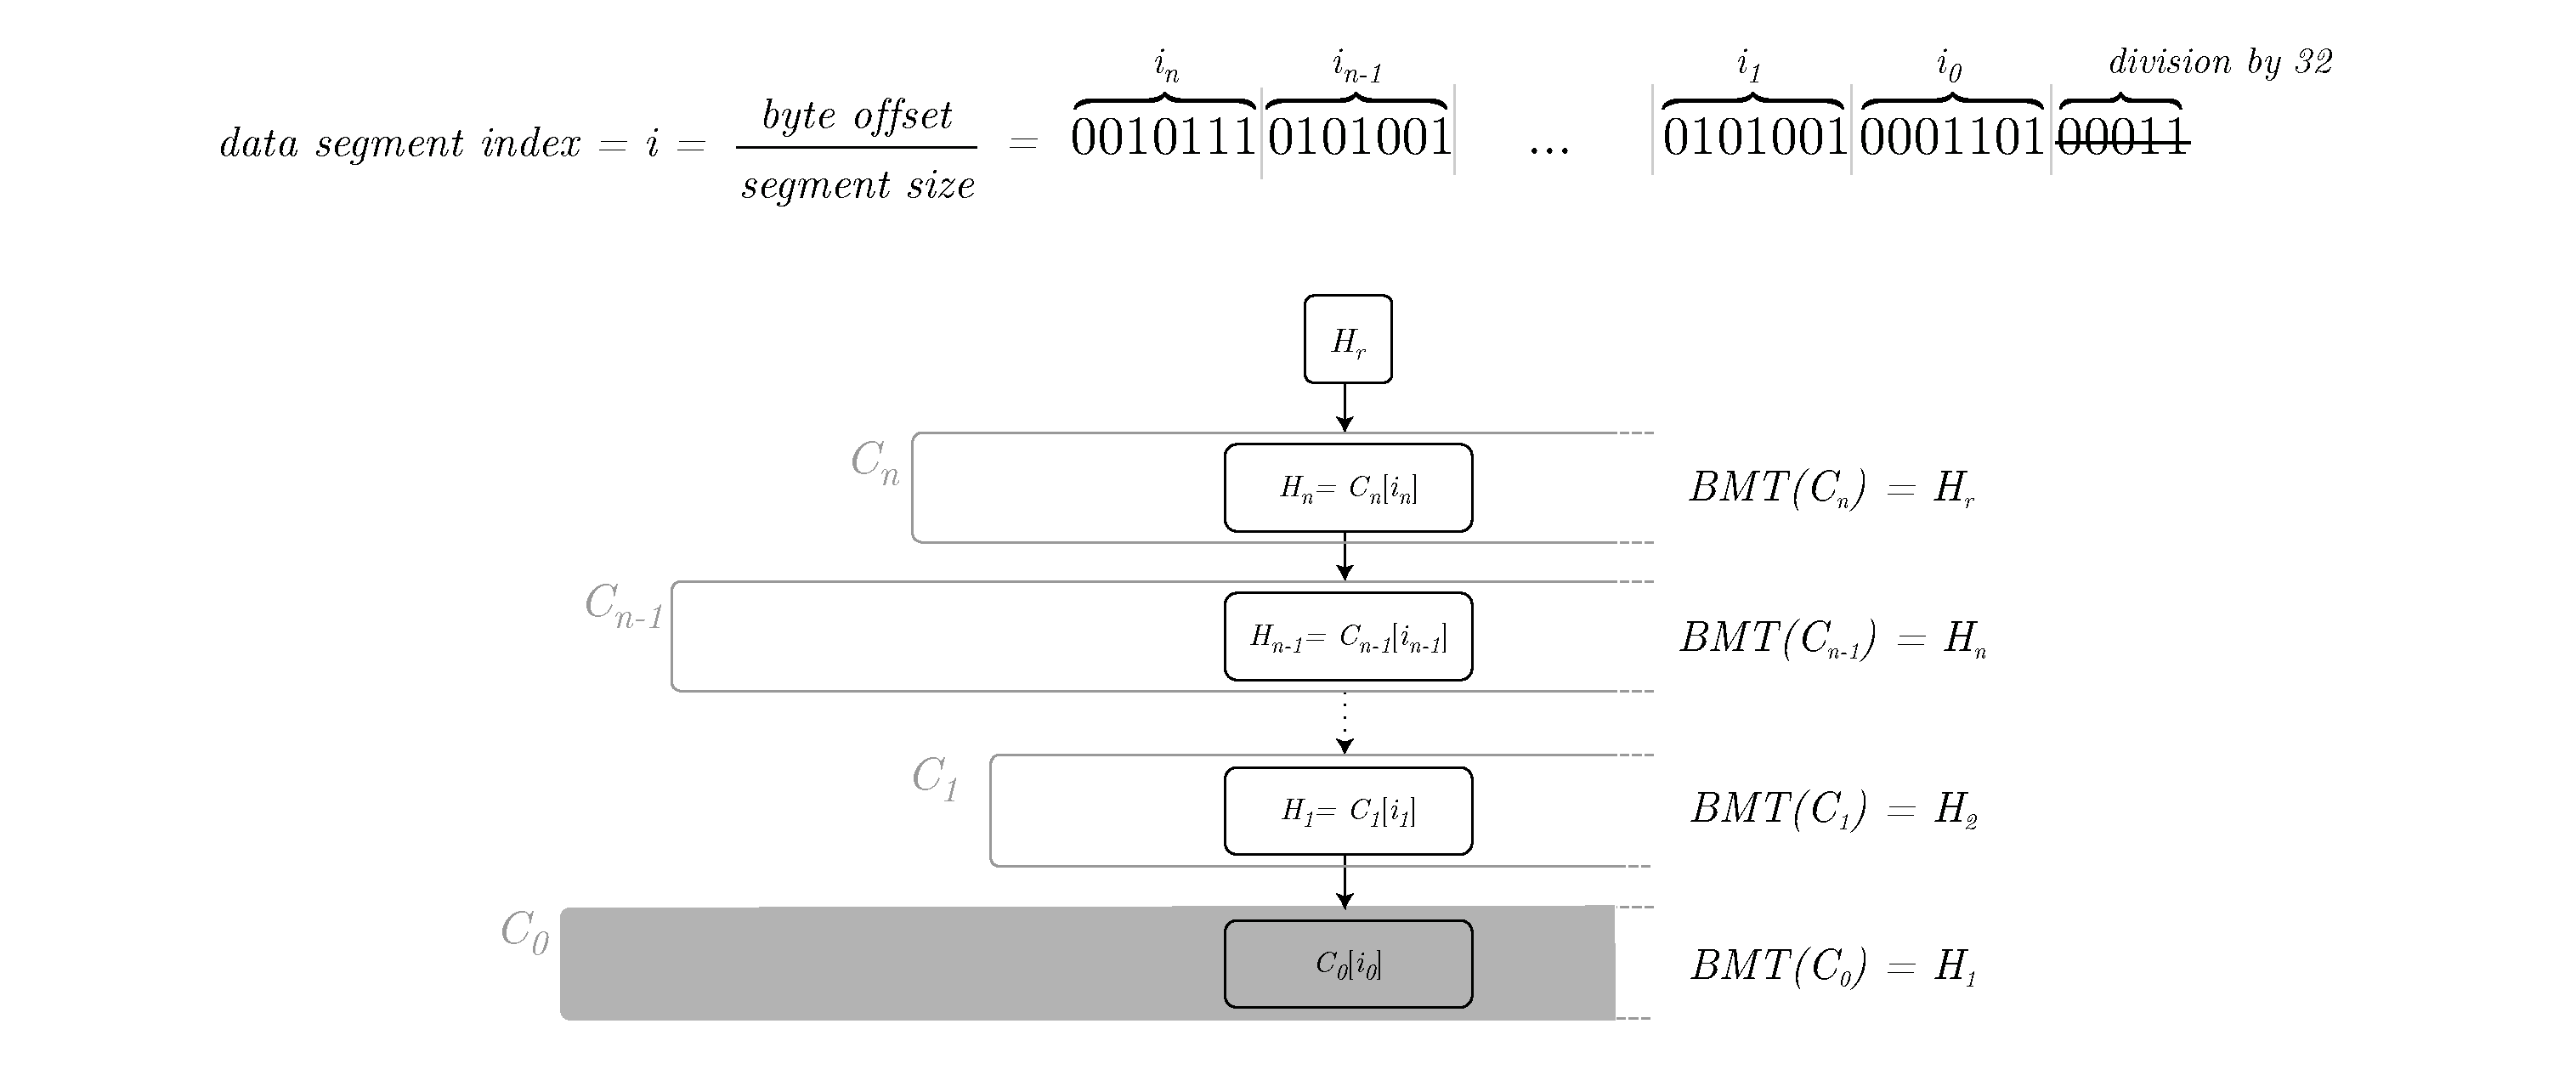
\includegraphics[width=\textwidth]{fig/random-access.pdf}
\caption[Random access at arbitrary offset with Swarm hash \statusgreen]{Random access at arbitrary offset with Swarm hash. The arbitrary offset informs us how to traverse the Swarm hash tree.}
\label{fig:random-access}
\end{figure}

\subsubsection{Compact inclusion proofs for files}


\begin{figure}[htbp]
\centering
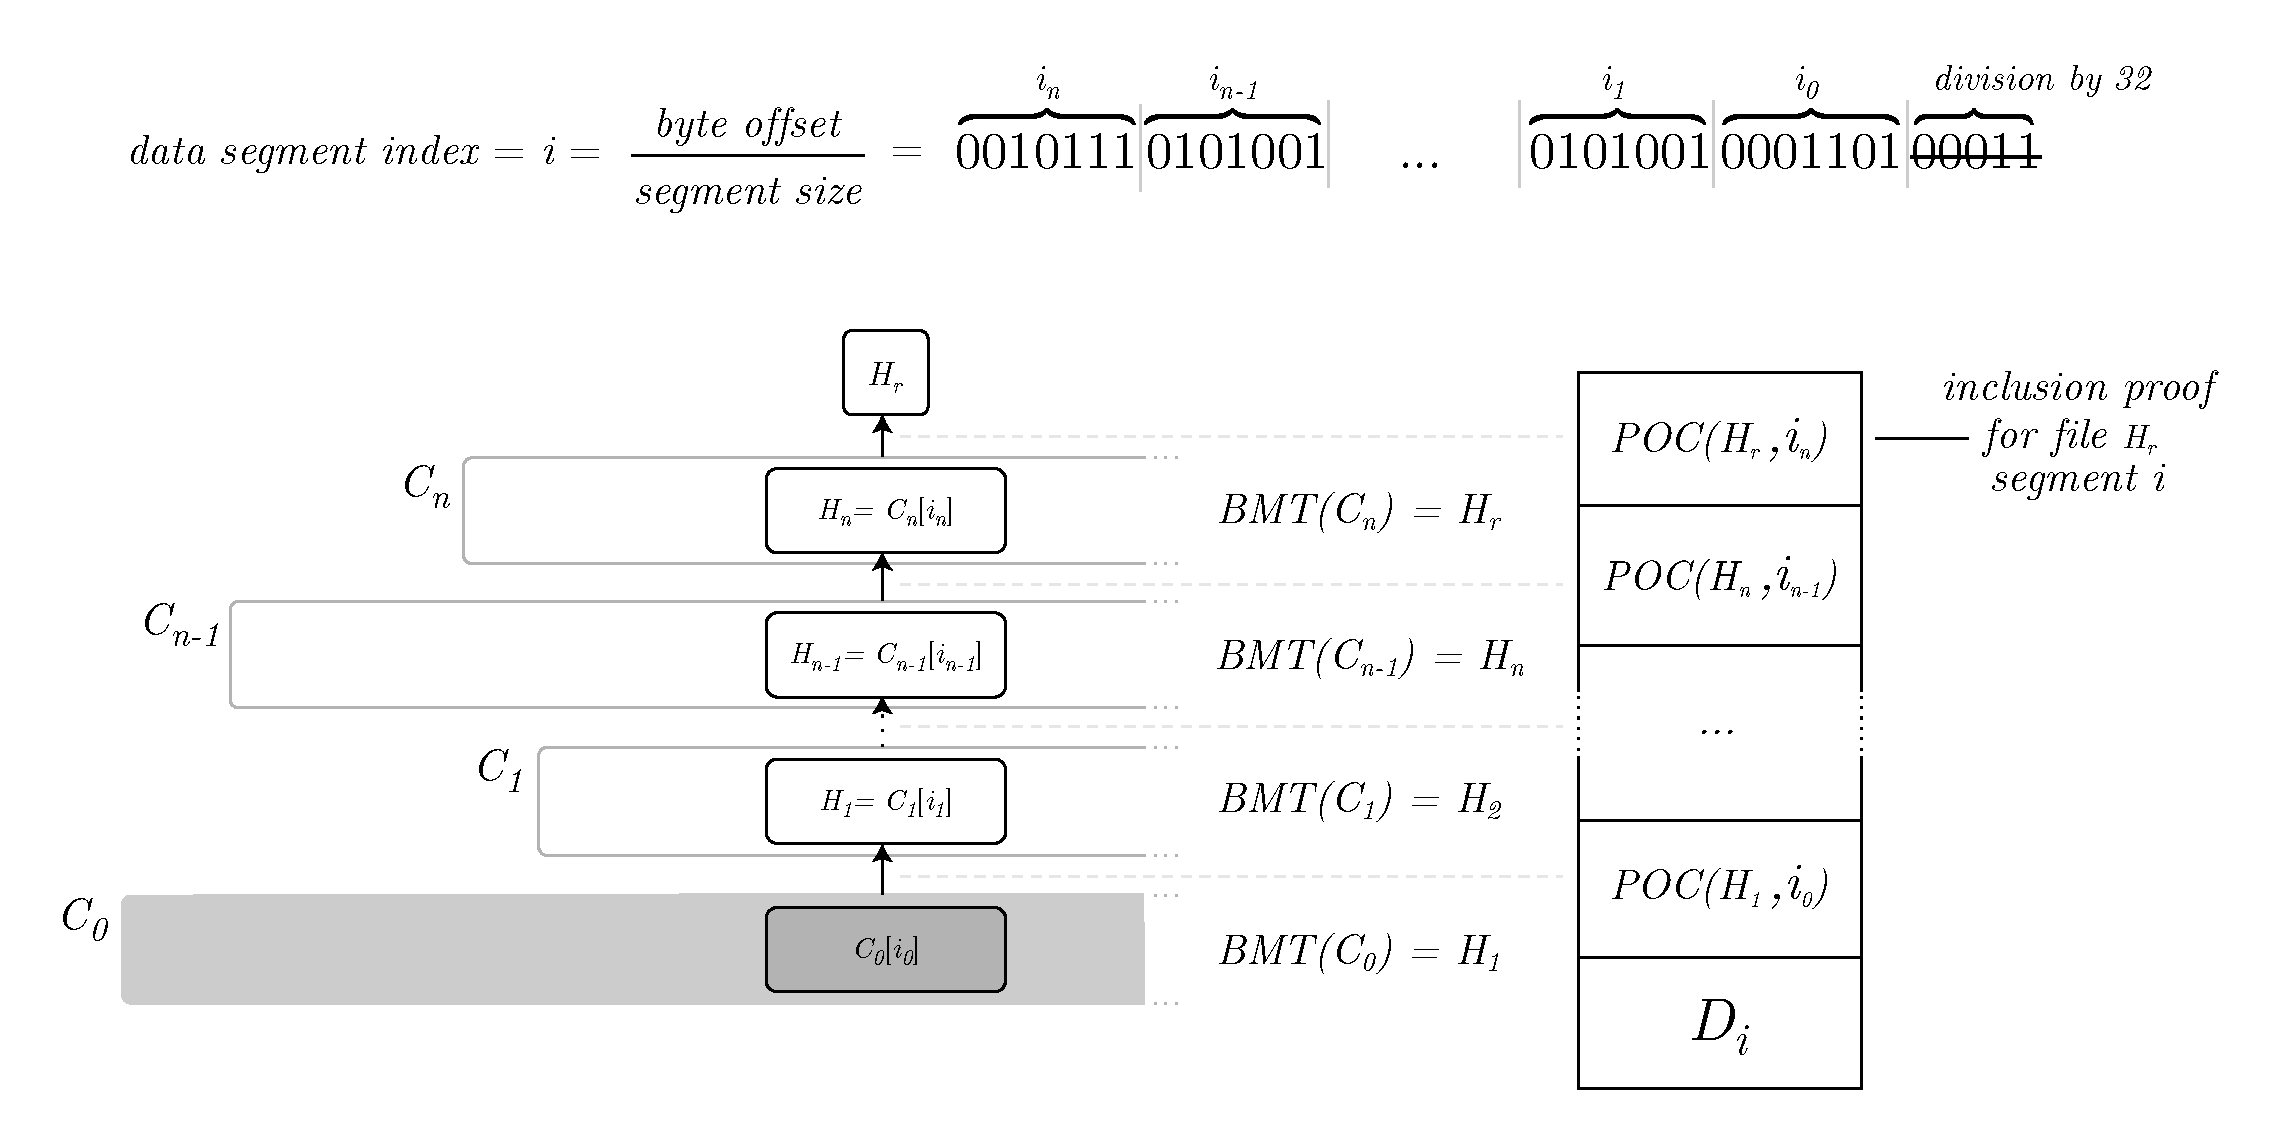
\includegraphics[width=\textwidth]{fig/file-inclusion.pdf}
\caption[Compact inclusion proofs for files \statusgreen]{Compact inclusion proofs for files. If we need to prove inclusion of segment   $i$, after division by 32 (within-segment position), we follow groups of 7 bits to find the respective segment of the intermediate node.}
\label{fig:file-inclusion}
\end{figure}


Suppose we were to prove the inclusion of a substring in a file at a particular offset. We saw that the offset applied to the data maps to a deterministic path traversing the Swarm hash. Since a substring inclusion proof simply reduces to a series of proofs of data segment paths, the chunk addresses are a result of a BMT hash where the base segments are 32-byte long. This means that in intermediate chunks, BMT base segments align with the addresses of children. As a consequence, proving that a the child of an intermediate chunk at a particular span offset is equivalent to giving a segment inclusion proof on the child hash. Therefore, substring inclusion in files can be proved with a sequence of BMT inclusion proofs (see \ref{spec:format:bmt}) where the length of the sequence corresponds to the depth of the Swarm hash tree (see figure \ref{fig:file-inclusion}). 


Note that such inclusion proofs are possible even in the case of encrypted data since the decryption key at for a segment position can be selectively disclosed without revealing any information that could compromise the encryption elsewhere in the chunk.

In this section, we presented Swarm hash, a data structure over chunks that represents files, which supports the following functionalities:

\begin{itemize}
    \item \emph{random access} -- The file can be read from any arbitrary offset with no extra cost.
    \item \emph{append} -- Supports append without duplication. 
    \item \emph{length preserving edits} -- Supports length preserving edits without duplication of unmodified parts.
    \item \emph{compact inclusion proofs} -- Allow inclusion proofs with resolution of 32 bytes in space logarithmic in file size.
\end{itemize}



\subsection{Collections and manifests\statusgreen}\label{sec:collections}

The \gloss{Swarm manifest} is a structure that defines a mapping between arbitrary paths and files to represent collections. It also contains metadata associated with the collection and its objects (files). A \gloss{manifest entry} contains a reference to a file, more precisely a reference to the Swarm root chunk of the representation of file (see \ref{sec:files}) and also specifies the media mime type of file so that browsers will know how to handle it. You can think of a manifest as (1) a routing table, (2) a directory tree, or  (3) an index, which makes it possible for Swarm to implement (1) web sites, (2) file-system directories, or (3) key--value stores (see \ref{sec:maps}), respectively. Manifests provide the main mechanism to enable URL based addressing in Swarm (see \ref{sec:urls}). 

Manifests are represented as a compacted trie%
%
\footnote{see \url{https://en.wikipedia.org/wiki/Trie}}
%
in which individual trie nodes are serialised as chunks (see \ref{spec:format:manifests}). The paths are associated with a \gloss{manifest entry} that specifies at least the \emph{reference}. The reference may then point to an embedded manifest if the path is a common prefix of more than one path in the collection, thereby implementing branching in the trie, see figure \ref{fig:manifest-structure}. 


\begin{figure}[htbp]
\centering
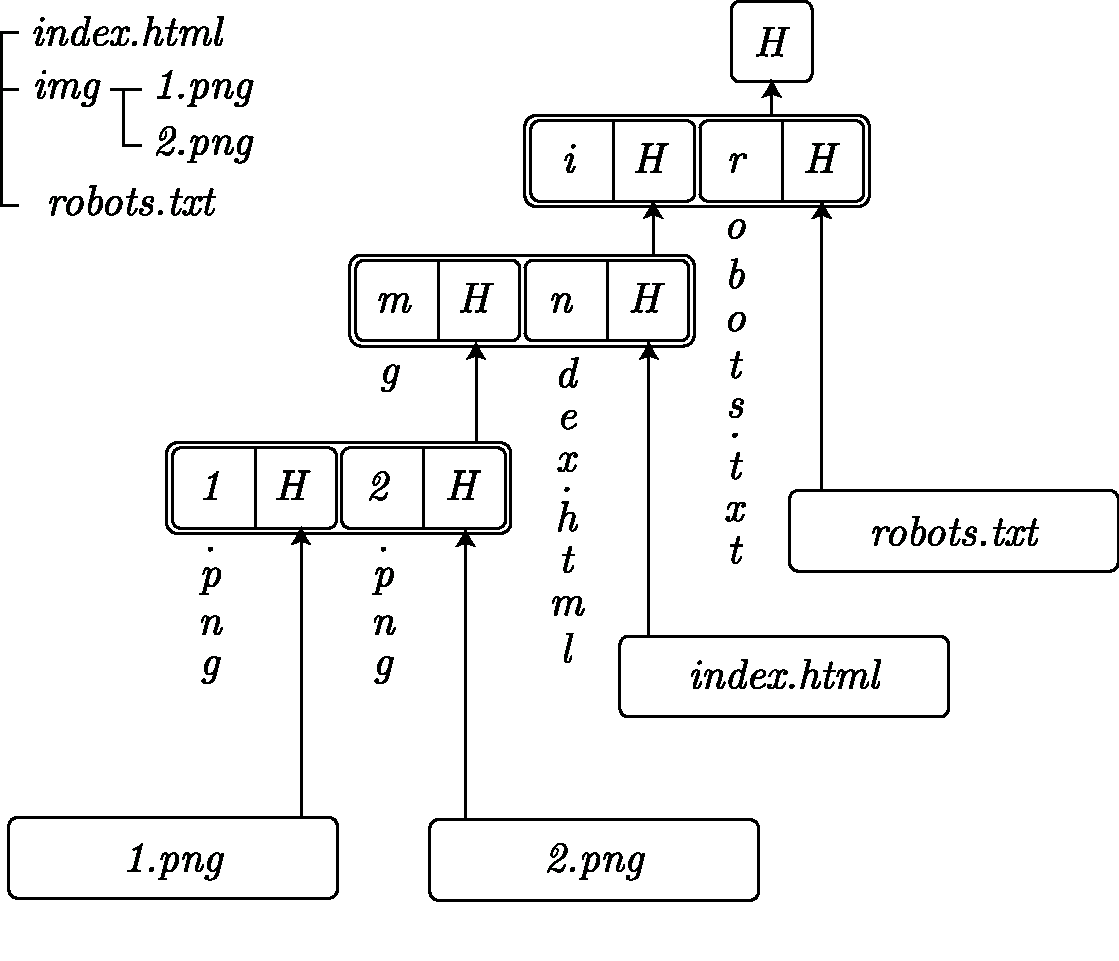
\includegraphics[width=0.7\textwidth]{fig/manifest-structure.pdf}
\caption[Manifest structure \statusgreen]{Manifest structure. Nodes represent a generic trie node: it contains the forks which describe continuations sharing a prefix. Forks are indexed by the next byte of the key, the value of which contains the Swarm reference to the child node as well as the longest prefix (compaction).}
\label{fig:manifest-structure}
\end{figure}

\begin{figure}[htbp]
\centering
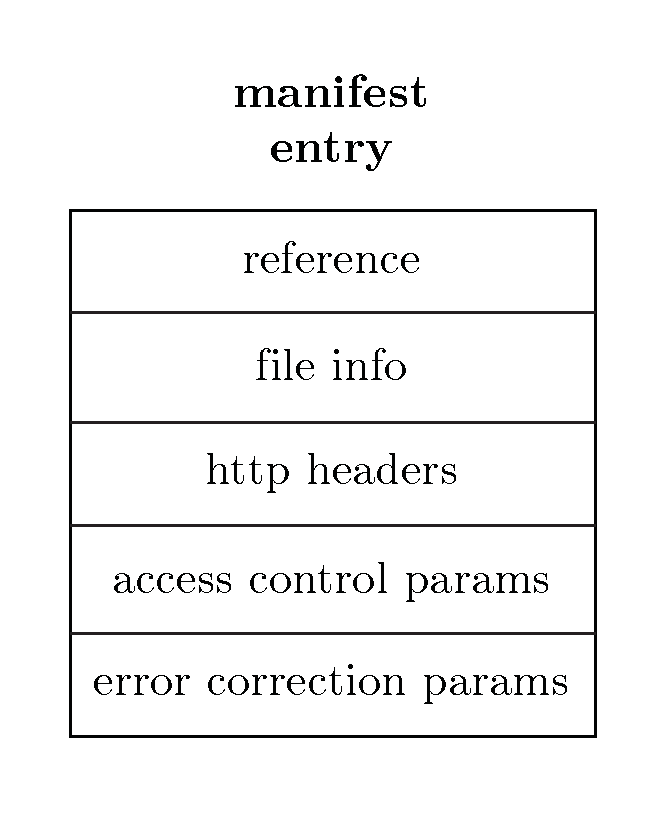
\includegraphics[width=\textwidth]{fig/manifest-entry.pdf}
\caption[Manifest entry \statusgreen]{Manifest entry is a data  structure that contains the reference to a file including metadata about a file or directory  pertaining to the assembler, access control and http headers.}
\label{fig:manifest-entry}
\end{figure}

A manifest entry is a data  structure that encapsulates all metadata about a file or directory.
The information minimally includes a swarm reference to the file, complemented with file information
relevant either as a (1) parameter for the downloader component which assembles chunks into a byte stream or (2) for the client side rendering handled by the browser or (3) for the mapping of manifests to file system directory tree. (1) is exemplified by access control information and erasure coding parameters but also the publisher needed for doing chunk recovery. (2) includes content type headers, or generically HTTP headers that the local swarm client will pick them up by the API and set in the response header when the file is retrieved. 
and (3) file info mapped to file system when downloading such as file permissions.

The high level API (see \ref{spec:api:storage}) to the manifests provides functionality to upload and download files and directories. It also provides an interface to add documents to a collection on a path and to delete a document from a collection. Note that deletion here only means that a new manifest is created in which the path in question is missing. There is no other notion of deletion in the Swarm, i.e. the value that was referenced in the deleted manifest entry remains in Swarm. Swarm exposes the manifest API via the \emph{bzz URL scheme} (see \ref{spec:api:storage}).

\subsection{URL-based addressing and name resolution\statusgreen}\label{sec:urls}

Earlier we introduced the low level network component of Swarm as a distributed immutable store of chunks (DISC, see \ref{sec:disc}). In the previous two sections we presented ways in which files (\ref{sec:files}) and collections (\ref{sec:collections}) can be represented in Swarm and referenced using chunk references. Manifests provide a way to index individual documents in a collection and this allows them to be considered a representation of web sites hosted in Swarm. The root manifests serve as the entry-point to virtually hosted sites on Swarm and are therefore analogous to hosting servers. In the current web, domain names resolve to the IP address of the host server, and the URL paths (of static sites) map to entries in the directory tree based on their path relative to the document root set for the host.
Analogously, in Swarm, domain names resolve to a reference to the root manifest and the URL paths map to manifest entries based on their path.  

When the HTTP API serves a URL, the following steps are performed:

\begin{enumerate}
    \item \emph{domain name resolution} -- Swarm resolves the host part to a reference to a root manifest,
    \item \emph{manifest traversal} -- recursively traverse embedded manifests along the path matching the URL path to arrive at a manifest entry,
    \item \emph{serving the file} -- the file referenced in the manifest entry is retrieved and rendered in the browser with headers (notably content type) taken from  the metadata of manifest entry.
\end{enumerate}

Swarm supports domain name resolution using the \gloss{Ethereum Name Service} (\gloss{ENS}). \gloss{ENS} is the system that, analogously to the DNS of the old web, translates human-readable names into system-specific identifiers, i.e. a reference in the case of Swarm.%
% TODO:  add references 
\footnote{RNS, name service for RIF OS on RSK is also supported.}
%
In order to use ENS, the Swarm node needs to be connected to an EVM-based blockchain supporting the Ethereum API (ETH mainnet, Ropsten, ETC, etc). 
Users of ENS can register a domain name on the blockchain and set it to resolve to a reference. This reference is most commonly the content hash of a public (unencrypted) manifest root. In the case that this manifest represents a directory containing the assets of a website, the default path for the hash may be set to be the desired root html page. When an ENS name is navigated to using a Swarm enabled browser or gateway, Swarm will simply render the root html page and Swarm will provide the rest of the assets provided in the relative path. In this way, users are able to very easily host websites, and Swarm provides an interface to older pre-existing browsers, as well as implementing a decentralised improvement over DNS.


\subsection{Maps and key--value stores\statusgreen}\label{sec:maps}

This section describes two ways of implementing a simple distributed key--value store in Swarm. Both rely solely on tools and APIs which have been already introduced.

One technique is by using manifests: Paths represent keys and the reference in the manifest entry with the particular path point to the value. This approach benefits from a full API enabling insert, update and remove through the bzz manifest API (see \ref{spec:api:storage}). Since manifests are structured as a compacted trie, this key--value store is scalable. Index metadata requires storage logarithmic to the number of key--value pairs. Lookup requires logarithmic bandwidth. The data structure allows for iteration that respects key order. 

Single-owner chunks also provide a way to define a key--value store.

This other technique simply posits that the index of the single owner chunk be constructed as a concatenation of the hash of the database name and the key. This structure only provides insert, no update or remove. Both insert and lookup are constant space and bandwidth. However, lookup is not safe against false negatives, i.e., if the chunk representing the key--value pair is not found, this does not mean it has never been created (e.g. it could have been garbage collected). Thus, the single owner chunk based key--value store is best used as (1) a bounded cache of recomputable values, (2) mapping between representations such as a translation between a Swarm hash and a Keccak256 hash as used in the Ethereum blockchain state trie nodes, or (3) conventional relational links, such as likes, upvotes and comments on a social media post. 


\section{Access control\statusgreen}\label{sec:access-control}

\green{}

This section first addresses the confidentiality of content using encryption. Encryption becomes especially useful once users are provided ways to manage other's access to restricted content. Use cases include managing private shared content as well as authorising access to a member's area of a web application. In this way we provide a robust and simple API to manage access control, something that is traditionally handled through centralised gate-keeping which is subject to frequent and disastrous security breaches.

\subsection{Encryption\statusgreen}\label{sec:encryption}

This section describes how to achieve confidentiality in a distributed public data storage. In this way, we show how to fulfill the natural requirement for many use cases to store private information and ensure that this is accessible only to specific authorised parties using Swarm. 

It is clear that the pseudo-confidentiality provided by the server-based access control predominantly used in current web applications is inadequate. In Swarm, nodes are expected to share the chunks with other nodes, in fact, storers of chunks are incentivised to serve them to anyone who requests them and therefore it is infeasible for nodes to act as the gatekeepers trusted with controlling access. Moreover, since every node could potentially be a storer, the confidentiality solution must leak nothing that allows third party storers to distinguish a private chunk from random data. As a consequence of this, the only way to prevent unauthorized parties from accessing private chunks is by using encryption. In Swarm, if a requestor is authorized to access a chunk, they must be in possession of a decryption key that can be used to decrypt the chunk, while unauthorized parties must not. Incidentally, this also serves as the basis for \gloss{plausible deniability}.

Encryption at the chunk level is described in \ref{sec:chunk-encryption} and formally specified in \ref{spec:format:encryption}. It 
has the desirable property that it is virtually independent of the chunk store layer, with the exact same underlying infrastructure for storing and retrieving chunks as the case of unencrypted content.
The only difference between accessing private and public data is the presence of a decryption/encryption key in the chunk references (see \ref{spec:format:files}) and the associated minor cryptographic computational overhead.

%, a constant or linear factor.

The storage API's raw \lstinline{GET} endpoint allows both encrypted and unencrypted chunk references. 
Decryption is triggered if the chunk reference is double size; consisting of the address of the encrypted chunk and a decryption key. Using the address, the encrypted chunk is retrieved, stored and decrypted using the supplied decryption key. The API responds with the resulting plaintext.

The storage API's \lstinline{POST} endpoint expects users to indicate if they want to have encryption on the upload or not. In both cases the chunk will be stored and push-synced to the network, but if encryption is desired, the encrypted chunk needs to be created first. If no further context is given, a random encryption key is generated which is used as a seed to generate random padding to fill the chunk up to a complete 4096 bytes if needed, and finally this plaintext is encrypted with the key. In the case of encryption, the API \lstinline{POST} call returns the Swarm reference consisting of the Swarm hash as chunk address and the encryption key. 

In order to guarantee the uniqueness of encryption keys as well as to ease the load on the OS's entropy pool, it is recommended (but not required) to generate the key as the \gloss{MAC} of the plaintext using a (semi-) permanent random key stored in memory. 
This key can be permanent and generated using \lstinline{scrypt} \cite{percival2009stronger}
with a password supplied upon startup. Instead of the plaintext, a namespace and path of the manifest entry can be used as context.
This use of a \gloss{key derivation function} has the consequence that chunk encryption will be deterministic as long as the context is the same: If we exchange one byte of a file and encrypt it with the same context, all data chunks of the file except the one that was modified will end up being encrypted exactly as the original (see \ref{spec:format:encryption}). Encryption is therefore deduplication friendly. 


\subsection{Managing access\statusgreen}\label{sec:managing-access}

This section describes the process the client needs to follow in order to obtain the full reference to the encrypted content. This protocol needs basic meta-information which is simply encoded as plaintext metadata and explicitly included in the root manifest entry for a document. This non-privileged access is called \gloss{root access}.

In contrast, \gloss{granted access} is a type of selective access requiring root access as well as access credentials: an authorised private key or passphrase. Granted access gives differentiated privileges for accessing the content by multiple parties sharing the same root access. This allows for updating the content without changing access credentials. Granted access is implemented using an additional layer of encryption on references.

The symmetric encryption of the reference is called the \gloss{encrypted reference}, the symmetric key used in this layer is called the \gloss{access key}.

In the case of granted access, the root access meta-information contains both the encrypted reference and the additional information required for obtaining the access key using the access credentials. Once the access key is obtained, the reference to the content is obtained by decrypting the encrypted reference with the access key, resulting in the full reference composed of the address root chunk and the decryption key for the root chunk. The requested data can then be retrieved and decrypted using the normal method.

The access key can be obtained from a variety of sources, three of which we will define.

\begin{figure}[htbp]
\centering
\includegraphics[width=\textwidth]{fig/access-control-single-party.pdf}
\caption[Access key as session key for single party access  \statusyellow]{Access key as session key for single party access.}
\label{fig:access-control-single-party}
\end{figure}

First, a \gloss{session key} is derived from the provided credentials. In the case of granting access to a single party, the session key is used directly as the access key, see figure \ref{fig:access-control-single-party}. In the case of multiple parties, an additional mechanism is used for turning the session key into the access key.

\subsubsection{Passphrase}
The simplest credential is a \emph{passphrase}. The session key is derived from a passphrase using \lstinline{scrypt} with parameters that are specified within the root access meta-information. The output of scrypt is a 32-byte key that may be directly used for Swarm encryption and decryption algorithms.

In typical use cases, the passphrase is distributed by an off-band means with adequate security measures, or exchanged in person. Any user knowing the passphrase from which the key was derived will be able to access the content.

\subsubsection{Asymmetric derivation}

A more sophisticated credential is a \emph{private key}, identical to those used throughout Ethereum for accessing accounts, i.e. an  elliptic curve using secp256k1. In order to obtain the session key, an \gloss{elliptic curve Diffie-Hellman} (\gloss{ECDH}) key agreement must be performed between the content publisher and the grantee. The resulting shared secret is hashed together with a salt. The content publisher's public key as well as the salt are included among metadata in the \gloss{root access manifest}. It follows from the standard assumptions of ECDH, that this session key can only be computed by the publisher and the grantee and no-one else. 
Once again, if access is granted to a single public key, the session key derived this way can be directly used as the access key which allows for the decryption of the encrypted reference. 
Figure \ref{fig:credentials-to-derive-session-key} summarises the use of credentials to derive the session key.

\begin{figure}[htbp]
\centering
\includegraphics[width=\textwidth]{fig/credentials-to-derive-session-key.pdf}
\caption[Credentials to derive session key  \statusyellow]{Credentials to derive session key.}
\label{fig:credentials-to-derive-session-key}
\end{figure}


\subsection{Selective access to multiple parties\statusgreen}

In order to manage access by multiple parties to the same content, an additional layer is introduced to obtain the access key from the session key. In this variant, grantees can be authenticated using either type of credentials, however, the session key derived as
described above is not used directly as the access key to decrypt the reference. Instead, two keys: a \gloss{lookup key} and an \gloss{access key decryption key}, are derived from it by hashing it with two different constants ($0$ and $1$, respectively).

When granting access, the publisher needs to generate a global access key to encrypt the full reference and then encrypt it with the
access key decryption keys for each grantee. Thereafter, a lookup table is created, mapping each grantees lookup key to their encrypted access key. Then, for each lookup key, the access key is encrypted with the corresponding access key decryption key.

This lookup table is implemented as an \gloss{access control trie} (\gloss{ACT}) in Swarm manifest format with paths corresponding to lookup keys and manifest entries containing the ciphertext of the encrypted access keys as metadata attribute values. The ACT manifest is an independent resource referenced by a URL which is included among the root access metadata so that users know whether or not an ACT is to be used. Its exact format is specified in \ref{spec:format:access-control}.

When accessing content, the user retrieves the root access meta data, identifies the ACT resource and then calculates their session key using either their passphrase and the scrypt parameters or the publisher public key and their private key and a salt. From the session key they can derive the lookup key by hashing it with $0$ and then retrieve the manifest entry from ACT. For this they will need to know the root of the ACT manifest and then use the lookup key as the URL path. If the entry exists, the user takes the value of the access key attribute in the form of a ciphertext that is decrypted with a key derived by hashing the session key with the constant $1$. The resulting access key can then be used to decrypt the encrypted reference included in the root access manifest, see figure \ref{fig:access-control-multiple-party}. Once we unlock the manifest root, all references contain the decryption key.

\begin{figure}[htbp]
\centering
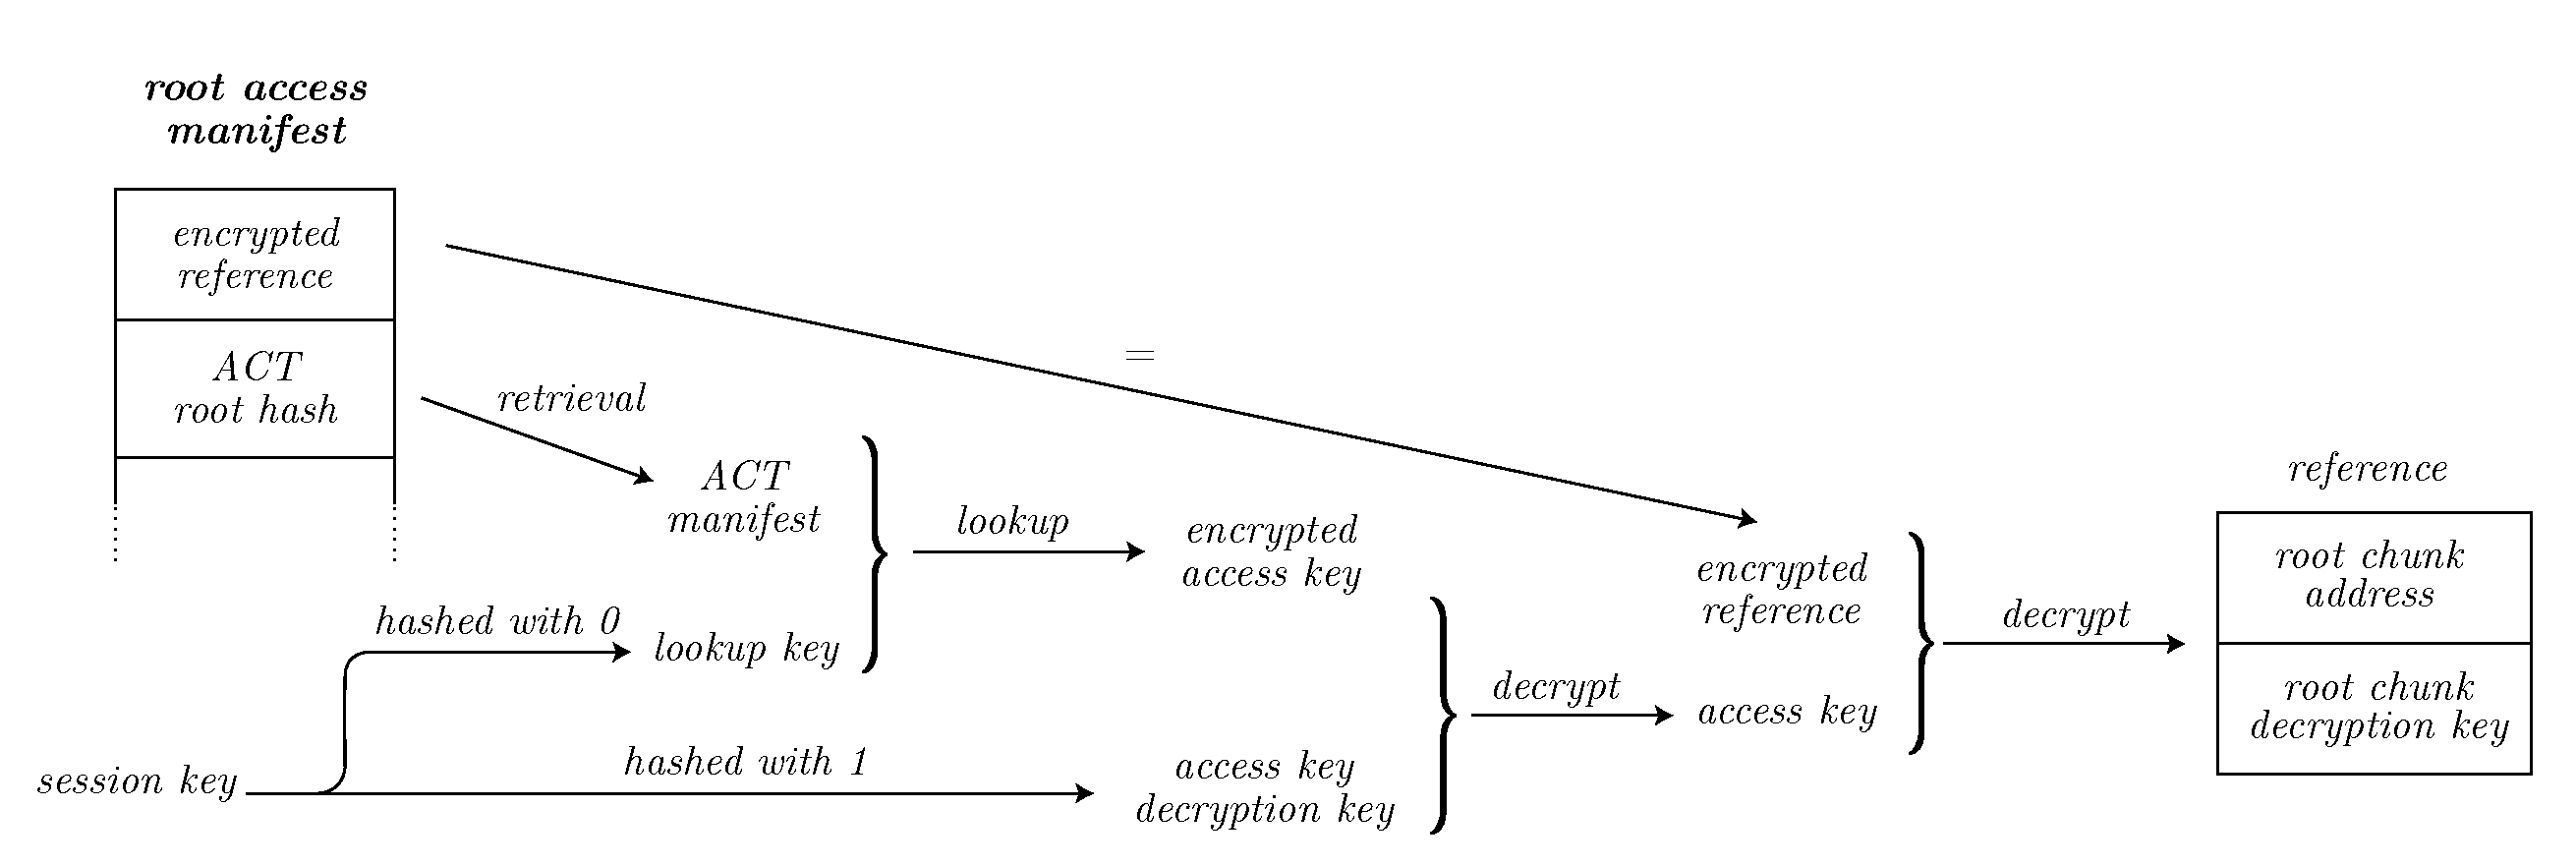
\includegraphics[width=\textwidth]{fig/access-control-multiple-party.pdf}
\caption[Access control for multiple grantees \statusyellow]{Access control for multiple grantees involves an additional layer to get from the session key to the access key. Each user must lookup the global access key specifically encrypted to them. Both the key to look up and the key to decrypt the access key are derived from the session key which in turn requires their credentials.} 
\label{fig:access-control-multiple-party}
\end{figure}


This access control scheme has a number of desirable properties:
\begin{itemize}
\item Checking and looking up one's own access is logarithmic in the size of the ACT.
\item The size of the ACT merely provides an upper bound on the number of grantees, but does not disclose any information beyond this upper bound about the set of grantees to third parties. Even those included in the ACT can only learn that they are grantees, but obtain no information about other grantees beyond an upper bound on their number.
\item Granting access to an additional key requires extending the ACT by a single entry, which is logarithmic in the size of the ACT. 
\item Withdrawing access requires a change in the access key and therefore the rebuilding of the ACT. Note that this also requires that the publisher retain a record of the public keys of the grantees after the initial ACT is created.
\end{itemize}

\subsection{Access hierarchy\statusgreen}

In the simplest case, the access key is a symmetric key. However, this is just a special case of the more flexible solution, where
the access key consists of a symmetric key and a key derivation path by which it is derived from a root key. In this case, in addition to the encrypted reference, a derivation path may also be included. Any party with an access key whose derivation is a prefix to the derivation path of the reference can decrypt the reference by deriving its key using their own key and the rest of the derivation path of the reference.

This allows for a tree-like hierarchy of roles, possibly reflecting an organizational structure. As long as role changes are "promotions", i.e. result in increase of privileges, it is sufficient to change a single ACT entry for each role change.

The exact format of manifests as well as the serialisation conventions are specified in more detail in \ref{spec:format:access-control}



\section{Swarm feeds and mutable resource updates \statusyellow}\label{sec:feeds}

\green{}

Feeds are a unique feature of Swarm. They constitute the primary use case for single owner chunks. Feeds can be used for versioning revisions of a mutable resource, indexing sequential updates to a topic, publish the parts to streams, or post consecutive messages in a communication channel to name but a few. Feeds implement persisted pull-messaging and can also be interpreted as a pub-sub system.
First, in \ref{sec:feed-chunks}, we introduce how feeds are composed of single owner chunks with an indexing scheme, the choice of which we discuss in \ref{sec:indexing-schemes}. In \ref{sec:feed-integrity}, we analyse why feed integrity is relevant and how it can be verified and enforced. \ref{sec:epoch-based-feeds} describe \gloss{epoch-based feeds} which provide feeds subject to receiving sporadic updates a way to be searched. Finally, in \ref{sec:feed-as-channel}, we show how feeds can be used as an outbox to send and receive subsequent messages in a communication channel.


\subsection{Feed chunks \statusyellow}\label{sec:feed-chunks}

A feed chunk is a single owner chunk with the associated constraint that the identifier is composed of the hash of a \gloss{feed topic} and a \gloss{feed index}. The topic is a 32-byte arbitrary byte array, this is typically the Keccak256 hash of one or more human readable strings specifying the topic and optionally the subtopic of the feed, see figure \ref{fig:feed-chunk}. 


\begin{figure}[htbp]
\centering
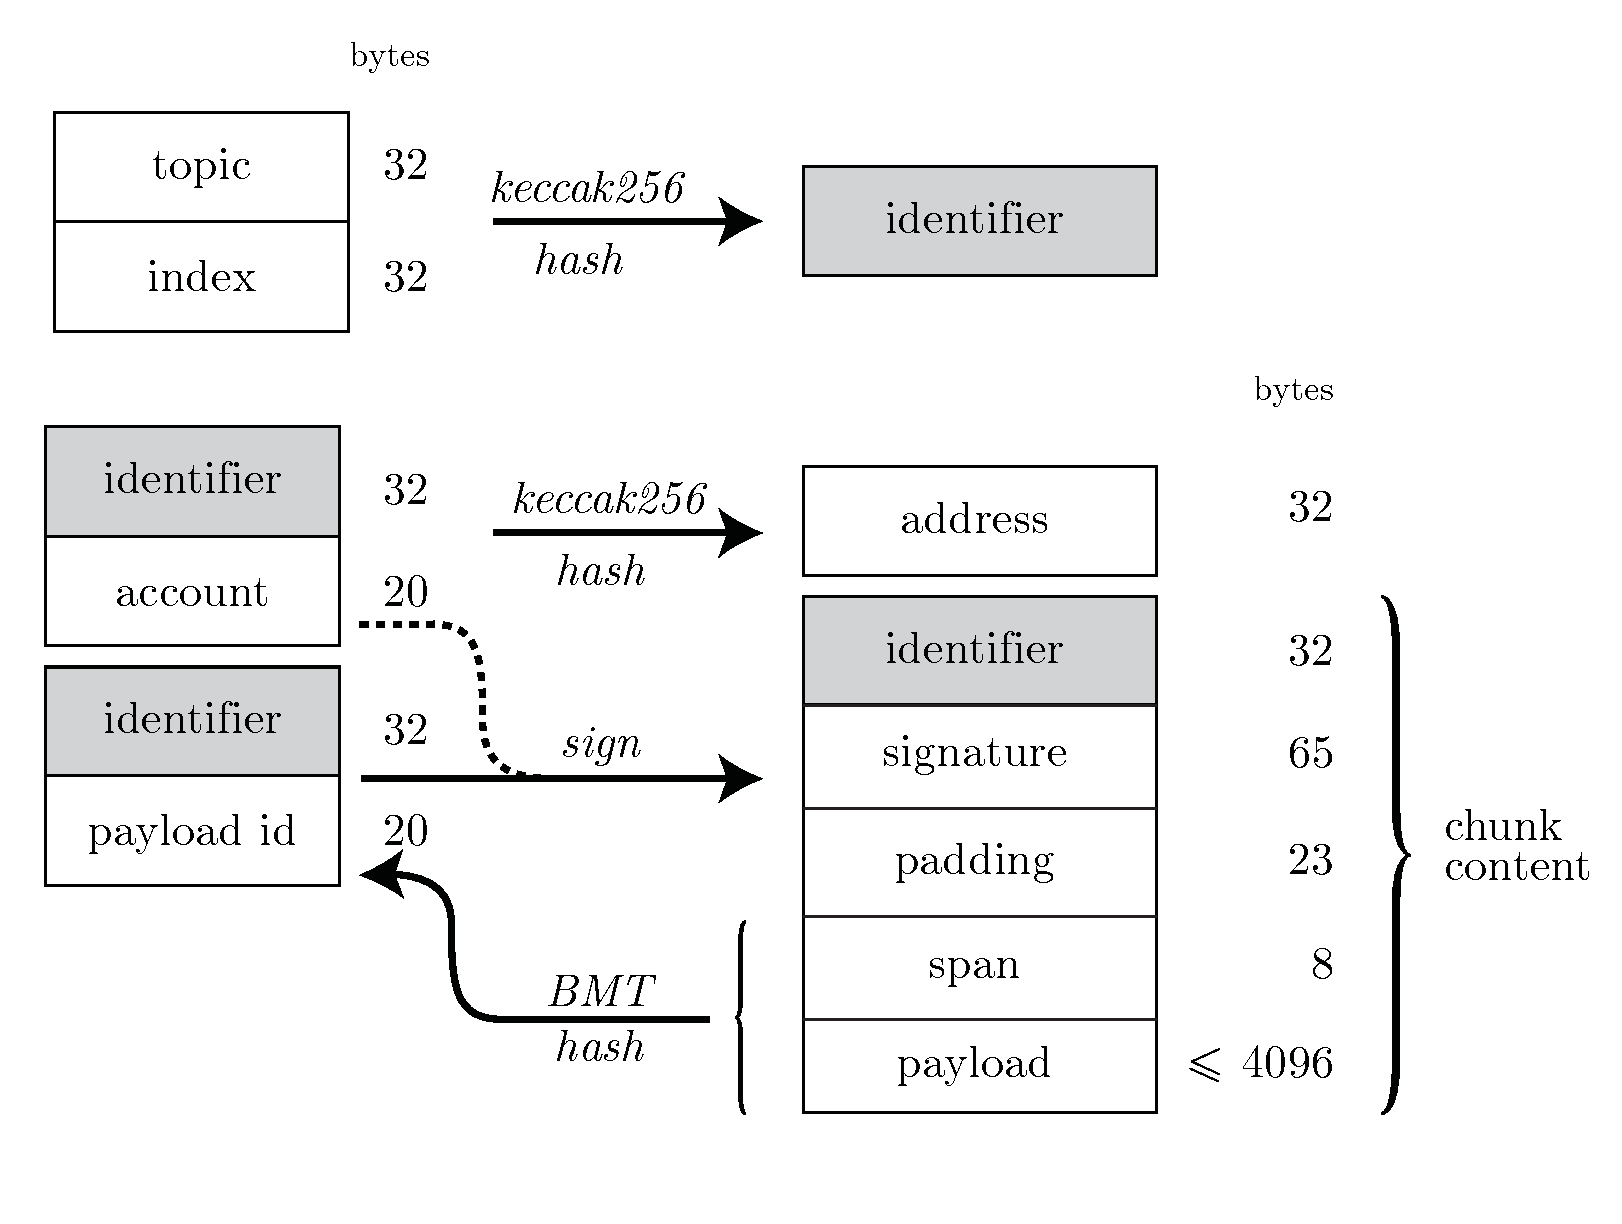
\includegraphics[width=\textwidth]{fig/feed-chunk.pdf}
\caption[Feed chunk \statusgreen]{Feed chunks are single owner chunks where the identifier is the hash of the topic and an index. Indexes are deterministic sequences calculated according to an indexing scheme. Subsequent indexes for the same topic represent identifiers for feed updates.}
\label{fig:feed-chunk}
\end{figure}

The index can take various forms defining some of the potentials types of feeds. The ones discussed in this section are: (1) simple feeds which use incremental integers as their index (\ref{sec:indexing-schemes}); (2)  \gloss{epoch-based feeds} which use an epoch ID (\ref{sec:epoch-based-feeds}); and (3) private channel feeds which use the nonces generated using a \gloss{double ratchet} key chain.  (\ref{sec:feed-as-channel}).
The unifying property of all these feed types is that both the publisher (owner) and the consumer must be aware of the \gloss{indexing scheme}. 

Publishers are the single owners of feed chunks and are the only ones able to post updates to their feed. Posting an update requires (1) constructing the identifier from the topic and the correct index and (2) signing it concatenated together with the hash of the arbitrary content of the update. Since the identifier designates an address in the owner's subspace of addresses, this signature effectively assigns the payload to this address (see \ref{sec:single-owner-chunks}). In this way, all items published on a particular feed are proven to have been created only by the owner of the associated private key.

Conversely, users can consume a feed by retrieving the chunk by its address. Retrieving an update requires the consumer to construct the address from the owner's public key and the identifier. To calculate the identifier they need the topic and the appropriate index. For this they need to know the indexing scheme. 

Feeds enable Swarm users to represent a sequence of content updates. The content of the update is the payload that the feed owner signs against the identifier. The payload can be a swarm reference from which the user can retrieve the associated data.

\subsection{Indexing schemes \statusyellow}\label{sec:indexing-schemes}

Different types of feeds require different \glossplural{indexing scheme} and different lookup strategies. In what follows, we introduce a few largely independent dimensions in which feeds can be categorised and which appear relevant in making a choice.


The actual indexing scheme used or even whether there is one (i.e. if the single owner chunk is a feed chunk at all) is left unrevealed in the structure of a feed chunk. As this information is not needed for the validation of a chunk by forwarding nodes, having the subtype explicit in the structure would leak  information unnecessarily. 

\subsubsection{Update semantics}

Updates of a feed can have three distinct semantics defining three subtypes of feeds. 
Revisions or mutable resource updates are \emph{substitutive}, series updates are \emph{alternative}, while partition updates are \emph{accumulative}. 

Feeds that represent revisions of the same semantic entity are called \gloss{mutable
resource updates}. These resources mutate because the underlying semantic entity changes such as versions of your CV or the resource description becomes more elaborate like the Wikipedia entry about a Roman emperor. Users will typically be interested in the latest update of such resources, past versions having only historical significance. 

A series of content connected by a common thread, theme or author such as status updates on social media, a person's blog posts or blocks of a blockchain can also be represented with feeds called \gloss{series}.
The updates in a series are interpreted as alternative and independent instantiations or episodes manifesting in temporal sequence. 

Finally, there are \gloss{partitions} expressed as feeds, updates of which are meant to be accumulated or added to earlier ones, for instance parts of a video stream. These mainly differ from series in that the feed updates are not interpretable on their own and the temporal sequence may represent a processing order corresponding to some serialisation of the structure of the resource rather than temporal succession. When such a feed is accessed, accumulation of all the parts may be necessary even for the integrity of the represented resource.

If subsequent updates of a feed include a reference to a data structure indexing the previous updates (e.g. a key--value store using the timestamp for the update or simply the root hash of the concatenation of update content), then the \gloss{lookup strategy} in all three cases reduces to looking up the latest update.

\subsubsection{Update frequency}

Within feeds which are updated over time may be several types, there are \gloss{sporadic feeds} with irregular asynchronicities, i.e. updates that can have unpredictable gaps and also \gloss{periodic feeds} with updates published at regularly recurring intervals.

We will also talk about \gloss{real-time feeds}, where the update frequencies may not be regular but do show variance within the temporal span of real-time human interaction, i.e. they are punctuated by intervals in the second to minute range.

\subsubsection{Subscriptions}

Feeds can be interpreted as \gloss{pub-sub systems} with persistence enabling asynchronous pulls. In what follows we analyse how the implementation of subscriptions to feeds as pub/sub is affected by the choice of \gloss{indexing scheme}.

In order to cater for subscribers to a feed, updates need to be tracked. If we know the latest update, periodic polling needs to be used to fetch the subsequent update. 
If the feed is periodic one can start polling after a known period. Alternatively, if the feed updates are frequent enough (at most a 1-digit integer orders of magnitude rarer than the desired polling frequency), then polling is also feasible.
However, if the feed is sporadic, polling may not be practical and we better resort to push notifications (see \ref{sec:trojan} and \ref{sec:notification-requests}).

If we missed out on polling for a period of time due to being offline, or just created the subscription, we can also rely on push notifications or use a \gloss{lookup strategy}. 

To look up partitions is not a problem since we need to fetch and accumulate each update, so in this case the strategy of just iterating over the successive indexes cannot be improved.
For periodic feeds, we can just calculate the index for a given time, hence asynchronous access is efficient and trivial. 
Looking up the latest version of a sporadically updated feed, however, necessitates some search and hence 
will benefit from \gloss{epoch-based indexing}.



\subsubsection{Aggregate indexing}

A set of sporadic feeds can be turned into a periodic one using \gloss{feed aggregation}. Imagine a multi-user forum like Reddit where each registered participant would publish comments on a post using sporadic feeds. In this scenario it is not practical for each user to monitor the comment feed of every other user and search through their sporadic feeds for updates in order to retrieve all the comments on the thread. It is much more efficient to just do it once though for all users. Indexers do exactly that and aggregate everyone's comments into an index, a data structure the root of which can now be published as a periodic feed, see figure \ref{fig:feed-aggregation}. The period can be chosen to give a real-time feed experience; even if the rate of change does not justify it, i.e. some updates will be redundant, the cost amortises over all users that use the aggregate feed and therefore is economically sustainable. 

\begin{figure}[htbp]
\centering
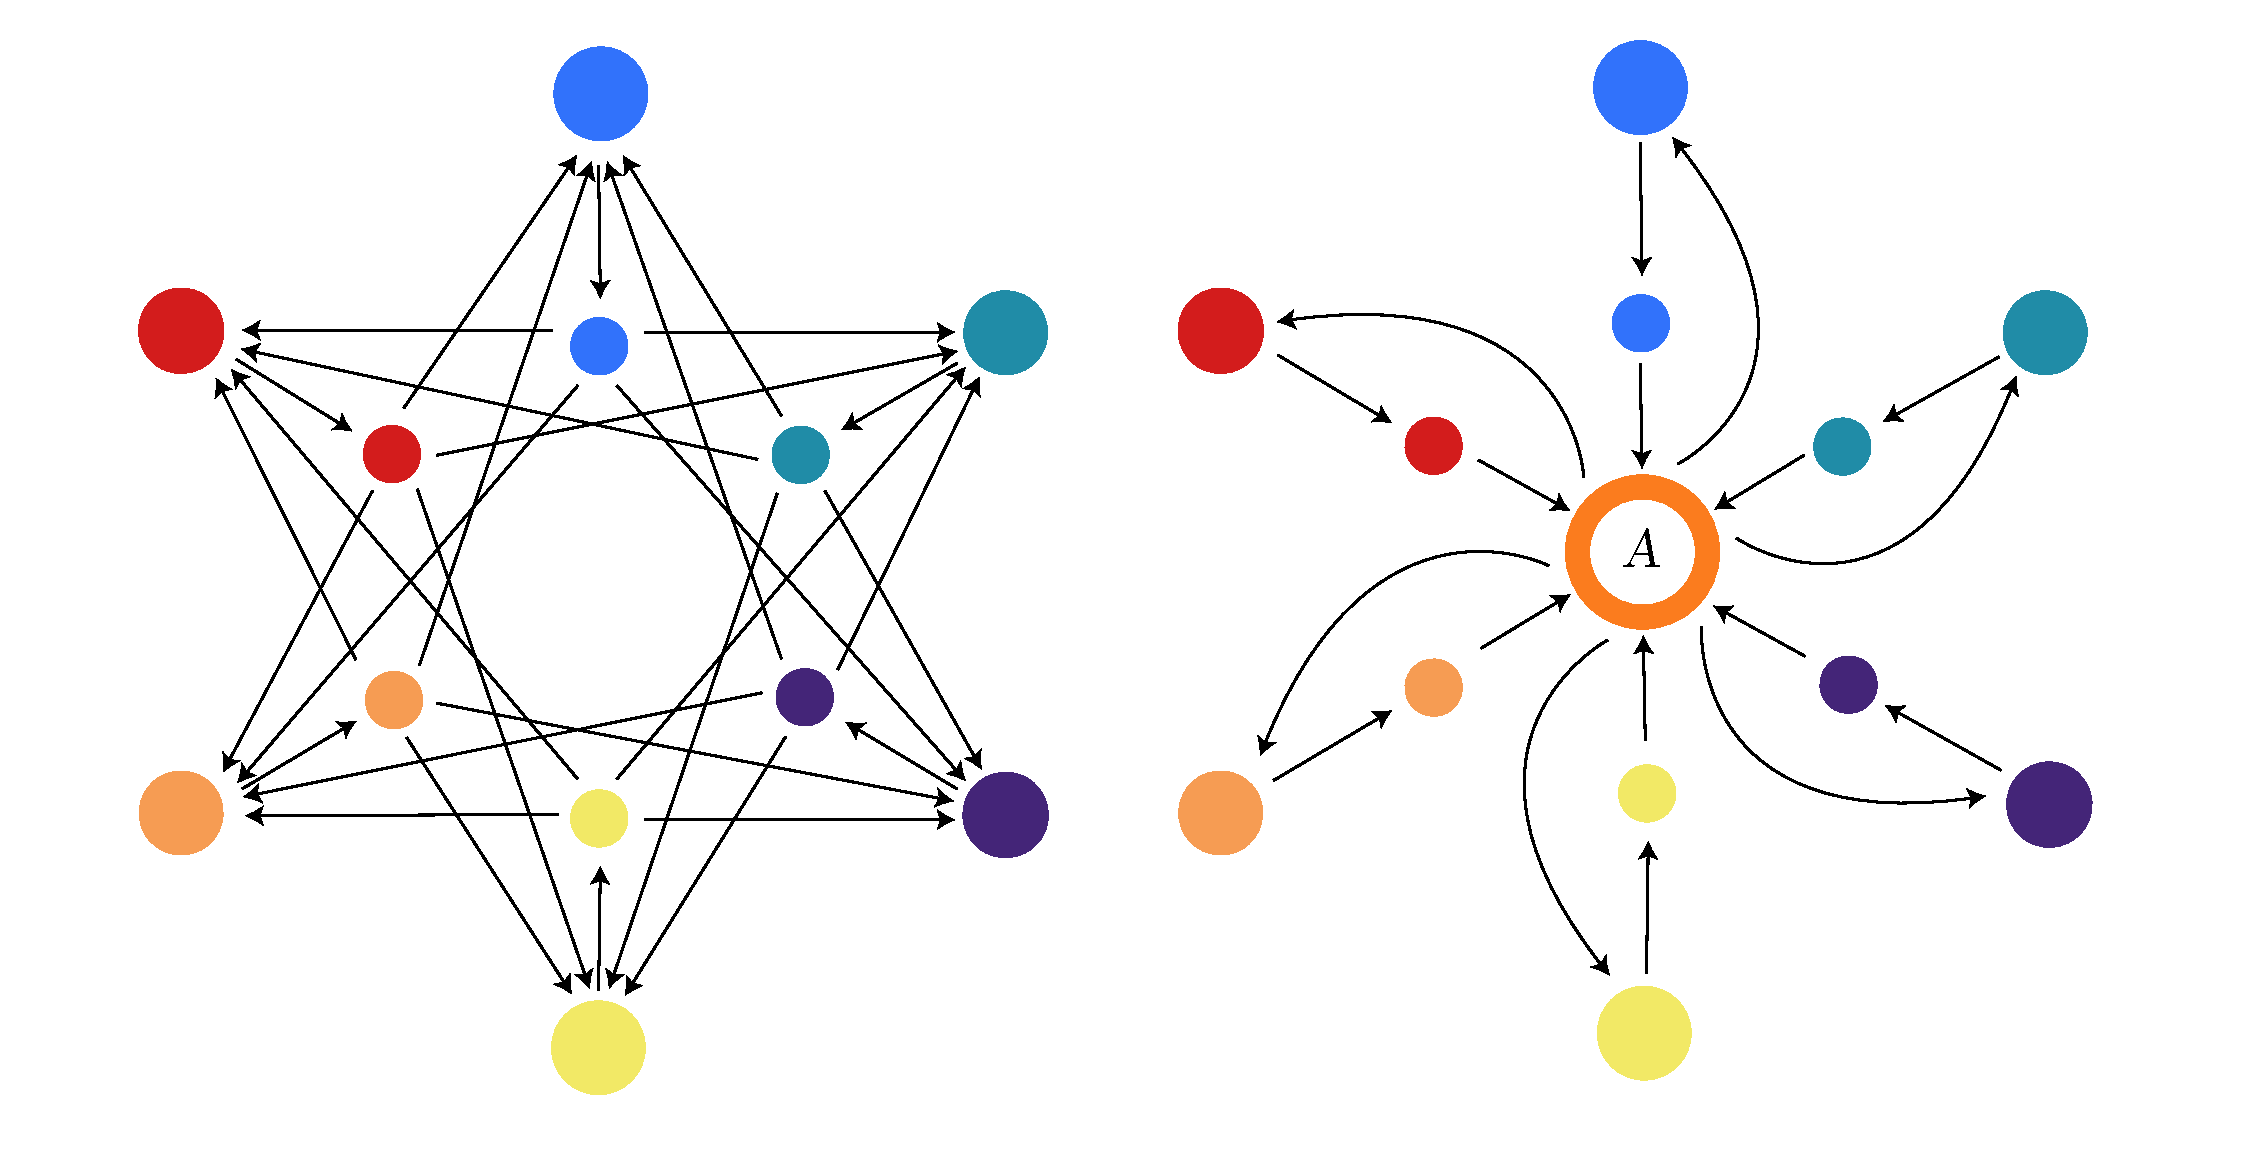
\includegraphics[width=\textwidth]{fig/feed-aggregation-2.pdf}
\caption[Feed aggregation \statusyellow]{Feed aggregation serves to merge information from several source feeds in order to save consumers from duplicate work. \textbf{Left:} 6 nodes involved in group communication (discussing a post, having real time chat, or asynchronous email thread). Each node publishes their contribution as outbox feed updates (small coloured circles). Each participant polls the other's epoch based feeds duplicating work with the lookup. \textbf{Right:} the 6 nodes now register  as sources  with an aggregator which polls the nodes' feed and creates indices that aggregate the sources into one data structure which each participant can then pull.}
\label{fig:feed-aggregation}
\end{figure}

Such a service can be provided with arbitrary levels of security, yet trustlessly without resorting to reputation. Using consensual data structures for the aggregation, incorrect indexes can be proved using cheap and compact inclusion proofs (see \ref{sec:files}) and therefore any challenge relating to correctness can be evaluated on chain. The threat of losing their deposit in case of an unrefuted challenge acts as a strong incentive for providers to maintain a good quality of service.

\subsection{Integrity \statusyellow}\label{sec:feed-integrity}

We say that a feed has \emph{integrity} if each of its updates has integrity, i.e. the update is unambiguous. Formally this means that for each index, the respective feed identifier is only ever assigned to a single payload. Incidentally, this also implies that the corresponding feed chunk has integrity. As discussed in \ref{sec:single-owner-chunks}, this is a prerequisite for consistent retrieval. 
If the payloads of the successive updates are imagined as blocks of a blockchain, then the criterion of integrity demands that feed owners must not fork their chain. 

In fact, the integrity of a feed can only be guaranteed by the owner. But can it be checked or enforced? Owners can commit to the integrity of their feeds by staking a deposit on the blockchain which they stand to lose if they are found to double sign on an update. Even though this may give a strong disincentive to fork a feed for long-term benefits, by itself, it is still unable to give sufficient guarantees to consumers of the feed with respect to integrity. Because of this, we must design indexing schemes which work to enforce this integrity.

\subsubsection{Authoritative version history}

Mutable resource update feeds track versions pretty much the same way as the Ethereum Name Service does.  
When the owner consolidates a version (say of a   website), they want to register the content address of the current version. In order to guarantee that there is no dispute over history, the payload needs to incorporate the previous payload's hash. This imposes the requirement that the payload must be a composite structure. If we want the payload to just be a manifest or manifest entry, so that it can be rooted to a path matching a URL, or directly displayed, this is not possible. Also, if the feed content is not a payload hash, then ENS registers a payload hash but the chunk may not exist on Swarm, so then the semantics of ENS are violated.

An indexing scheme which incorporates the previous payload hash into the subsequent index behaves like a blockchain in that it expresses the owner's unambiguous commitment to a particular history and that any consumer reading and using it expresses their acceptance of such a history. 
Looking up such feeds is only possible by retrieving each update since the last known one. The address is that of the update chunk, so registering the update address both guarantees historic integrity and preserves ENS semantics so that the registered address is just a Swarm reference to a chunk.
Such feeds implement an \gloss{authoritative version history}, i.e. a secure audit trail of the revisions of a mutable resource. 

\subsubsection{Real-time integrity check}

A deterministically indexed feed enables a \gloss{real-time integrity check}. In the context of feeds that represent blockchains (ledgers/side-chains), integrity translates to a non-forking and unique chain commitment. The ability to enforce this in real-time allows fast and secure definitions of transaction finality. 

We illustrate this with an example of an off-chain p2p payment network where each node's locked up funds are allocated to a fixed set of creditors (see more detail in \cite{ethersphere2019swap}). Creditors of the node need to check the correctness of reallocations, i.e. that the total increases are  covered by countersigned decreases. 
If a debitor keeps publishing a deposit allocation table for an exhaustive list of creditors, by issuing two alternatives to targeted creditors, the debitors will be able to orchestrate a double spend. Conversely, certainty in the uniqueness of this allocation table allows the creditor to conclude finality.

We claim that using Swarm feeds, this uniqueness constraint can be checked real time.

The insight here is that it is impossible to meaningfully control the responses to a single owner chunk request: There is no systematic way to respond with particular versions to particular requestors even if the attacker controls the entire neighbourhood of the chunk address.%
%
\footnote{If the chunks are uploaded using the same route, the chunk that comes later will be rejected as already known. If the two chunks originate from different addresses in the network, they might both end up in their local neighbourhood. This scenario will result in inconsistent retrievals depending on which node the request ends up with.}
%
This is the result of the ambiguity of the originator of the request due to the nature of forwarding Kademlia. Let us imagine that the attacker, with some sophisticated traffic analysis, has the chance of $1/n$ (asymptotic ceiling) to identify the originator and give a differential response. Sending multiple requests from random addresses, however, one can test integrity and consider a consistent response a requirement to conclude finality. The chance that the attacker can give a consistent differential response to a creditor testing with $k$ independent requests is $1/n^k$. With linear bandwidth cost in $k$, we can achieve exponential degrees of certainty about the uniqueness of an update. If a creditor finds consistency, it can conclude that there is no alternative allocation table.


By requiring the allocation tables to be disseminated as feed updates, we can leverage permissionlessness, availability and anonymity to enforce feed integrity. If the feed is a blockchain-like ledger, a real-time integrity check translates to fork finality. 


\subsection{Epoch-based 
indexing \statusyellow}\label{sec:epoch-based-feeds}

\yellow{}

In order to use single owner chunks to implement feeds with flexible update frequency, we introduce \gloss{epoch-based feeds}, an indexing scheme where the single owner chunk's identifier incorporates anchors related to the time of publishing. In order to be able to find the latest update, we introduce
an adaptive lookup algorithm. 

\subsubsection{Epoch grid}

An \gloss{epoch} represents a concrete time period starting at a specific point in time, called the \gloss{epoch base time} and has a specific length.  
Period lengths are expressed as powers of 2 in seconds. The shortest period is $2^0 = 1$ second, the longest is $2^{31}$ seconds. 

An \gloss{epoch grid} is the arrangement of epochs where rows (referred to as levels) represent alternative partitioning of time into various disjoint epochs with the same length. Levels are indexed by the logarithm of the epoch length putting level 0 with 1 second epoch length at the bottom by convention, see figure \ref{fig:epoch-grid}.

\begin{figure}[htbp]
\centering
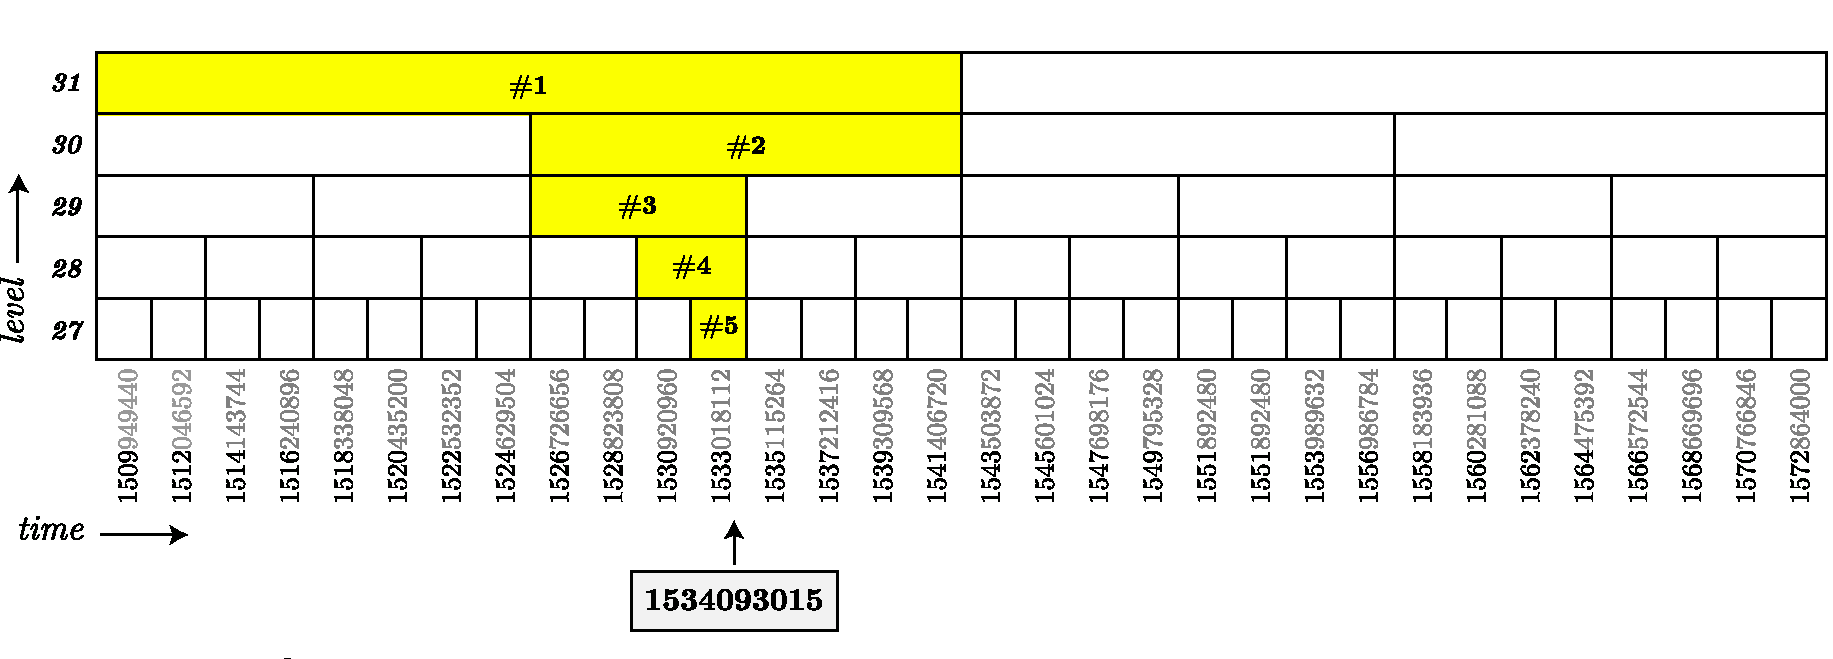
\includegraphics[width=\textwidth]{fig/epoch-grid.pdf}
\caption[Epoch grid with epoch-based feed updates\statusorange]{Epoch grid showing the first few updates of an epoch-based feed. Epochs occupied are marked in yellow and are numbered to reflect the order of updates they represent. }
\label{fig:epoch-grid}
\end{figure}

When representing a epoch-based feed in an epoch grid, each update is assigned to a different epoch in the grid based on their timestamp. In particular, an update is mapped to the longest free epoch that includes the timestamp. This structure gives the series of updates a contiguous structure which allows for easy search. The contiguity requirement implies that by knowing the epoch of the previous update, a subsequent update can be mapped to an epoch unambiguously.


To identify a specific epoch, we need to know both the epoch base time and the level. This pair is called the  \gloss{epoch reference}. To calculate the epoch base time of any given instant in time $t$ at a particular level $l$, we are dropping the $l$ least significant bits of $t$. 
The level requires one byte, and the epoch base time (using linux seconds) 4 bytes so the epoch reference can be serialised in 5 bytes. 
The epoch reference of the very first update of any epoch-based feed is always the same.

\subsubsection{Mapping epochs to feed update chunks}

Feed updates can then be mapped to feed chunks using the serialised epoch reference as the \gloss{feed index}. The topic of the feed hashed together with the index results in the feed identifier used in constructing the single owner chunk that expresses the feed chunk. 

To determine the epoch in which to store a subsequent update, the publisher needs to know where they stored the previous update. If the publisher does not keep track of this, they can use the lookup algorithm to find their last update.



\subsubsection{Lookup algorithm}

When consumers retrieve feeds, they typically will either want to look up the state of the feed at a particular time (historical lookup) or to find the latest update.

If historical lookups based on a \emph{target} time are required, the update can incorporate a data structure mapping timestamps to states. In such cases, finding any update later than the target can be used to deterministically look up the state at an earlier time. 

If no such index is available, historical lookups need to find the shortest filled epoch whose timestamp is earlier than the target. 

To select the best starting epoch from which to walk our grid, we have to assume the worst case scenario, which is that the resource was never again updated after we last saw it. If we don't know when the resource was last updated, we assume 0 as the "last time" it was updated.

We can guess a start level as the position of the first nonzero bit of $\mathit{lastUpdate}\xor \mathit{NOW}$ counting from the left. The bigger the difference among the two times (last update time and now), the higher the level will be.

In \ref{sec:epoch-based-feeds-appendix}, we walk the reader through an example.

\subsection{Real-time data exchange \statusyellow}\label{sec:feed-as-channel}

Feeds can be used to represent a communication channel, i.e. the outgoing messages of a persona. Such a feed, called an \gloss{outbox feed} can be created to provide email-like communication or instant messaging, or even the two combined. For email-like asynchronicities, \gloss{epoch-based indexing} can be used while for instant messaging, it is best to use deterministic sequence indexing. 
In group chat or group email, confidentiality is handled using an access control trie over the data structure, indexing each party's contribution to the thread. Communication clients can retrieve each group member's feed relating to a thread and merge their timelines for rendering. 

Even forums could be implemented with such an outbox mechanism, however, above a certain number of registered participants, aggregating all outboxes on the client side may become impractical and require index aggregators or other schemes to crowdsource combination of the data.

\subsubsection{Two-way private channels}
 
Private two-party communication can also be implemented using outbox feeds, see figure \ref{fig:feeds-as-channel}. The parameters of such feeds are set as part of an initial key exchange or registration protocol (see \ref{sec:pss-key-exchange}) which ensures that the parties consent on the indexing scheme as well as the encryption used. 


\begin{figure}[htbp]
  \centering
  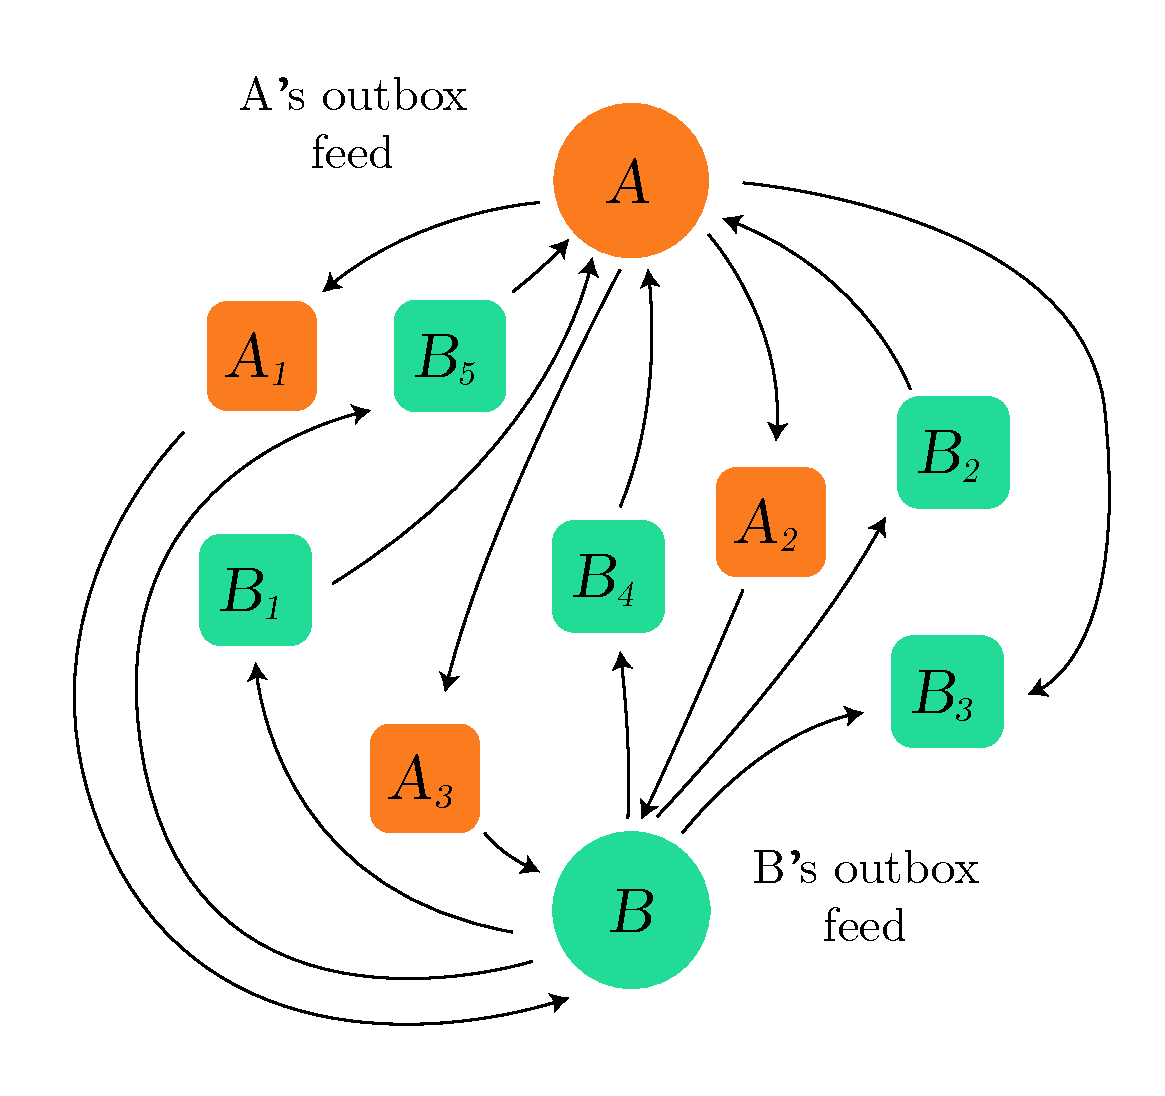
\includegraphics[width=0.7\textwidth]{fig/feeds-as-channel.pdf}  
  \caption[Swarm feeds as outboxes \statusgreen]{Swarm feeds as outboxes for private communication. Outbox feeds represent consecutive messages from a party in a conversation. The indexing scheme can follow a key management system with strong privacy which obfuscates the communication channel itself and renders interception attacks prohibitively expensive.}
\label{fig:feeds-as-channel}
\end{figure}


The real-time series feed used for instant messaging ought to have an indexing scheme with deterministic continuations for at least a few updates ahead. This enables sending retrieve requests for future updates ahead of time, i.e. during or even prior to processing the previous messages. When such retrieve requests arrive at the nodes whose address is closest to the requested update address, the chunk will obviously not be able to be found as the other party will not have sent them yet. However, even these storer nodes are incentivised to keep retrieve requests alive until they expire (see the argument in \ref{sec:retrieval}). This means that up until the end of their time-to-live setting (30 seconds), requests will behave as subscriptions: the arrival of the update chunk triggers the delivery response to the open request as if it was the notification sent to the subscriber. This reduces the expected message latency down to less than twice the average time of one-way forwarding paths, see figure \ref{fig:outbox-feed-latency}. 


\begin{figure}[htbp]
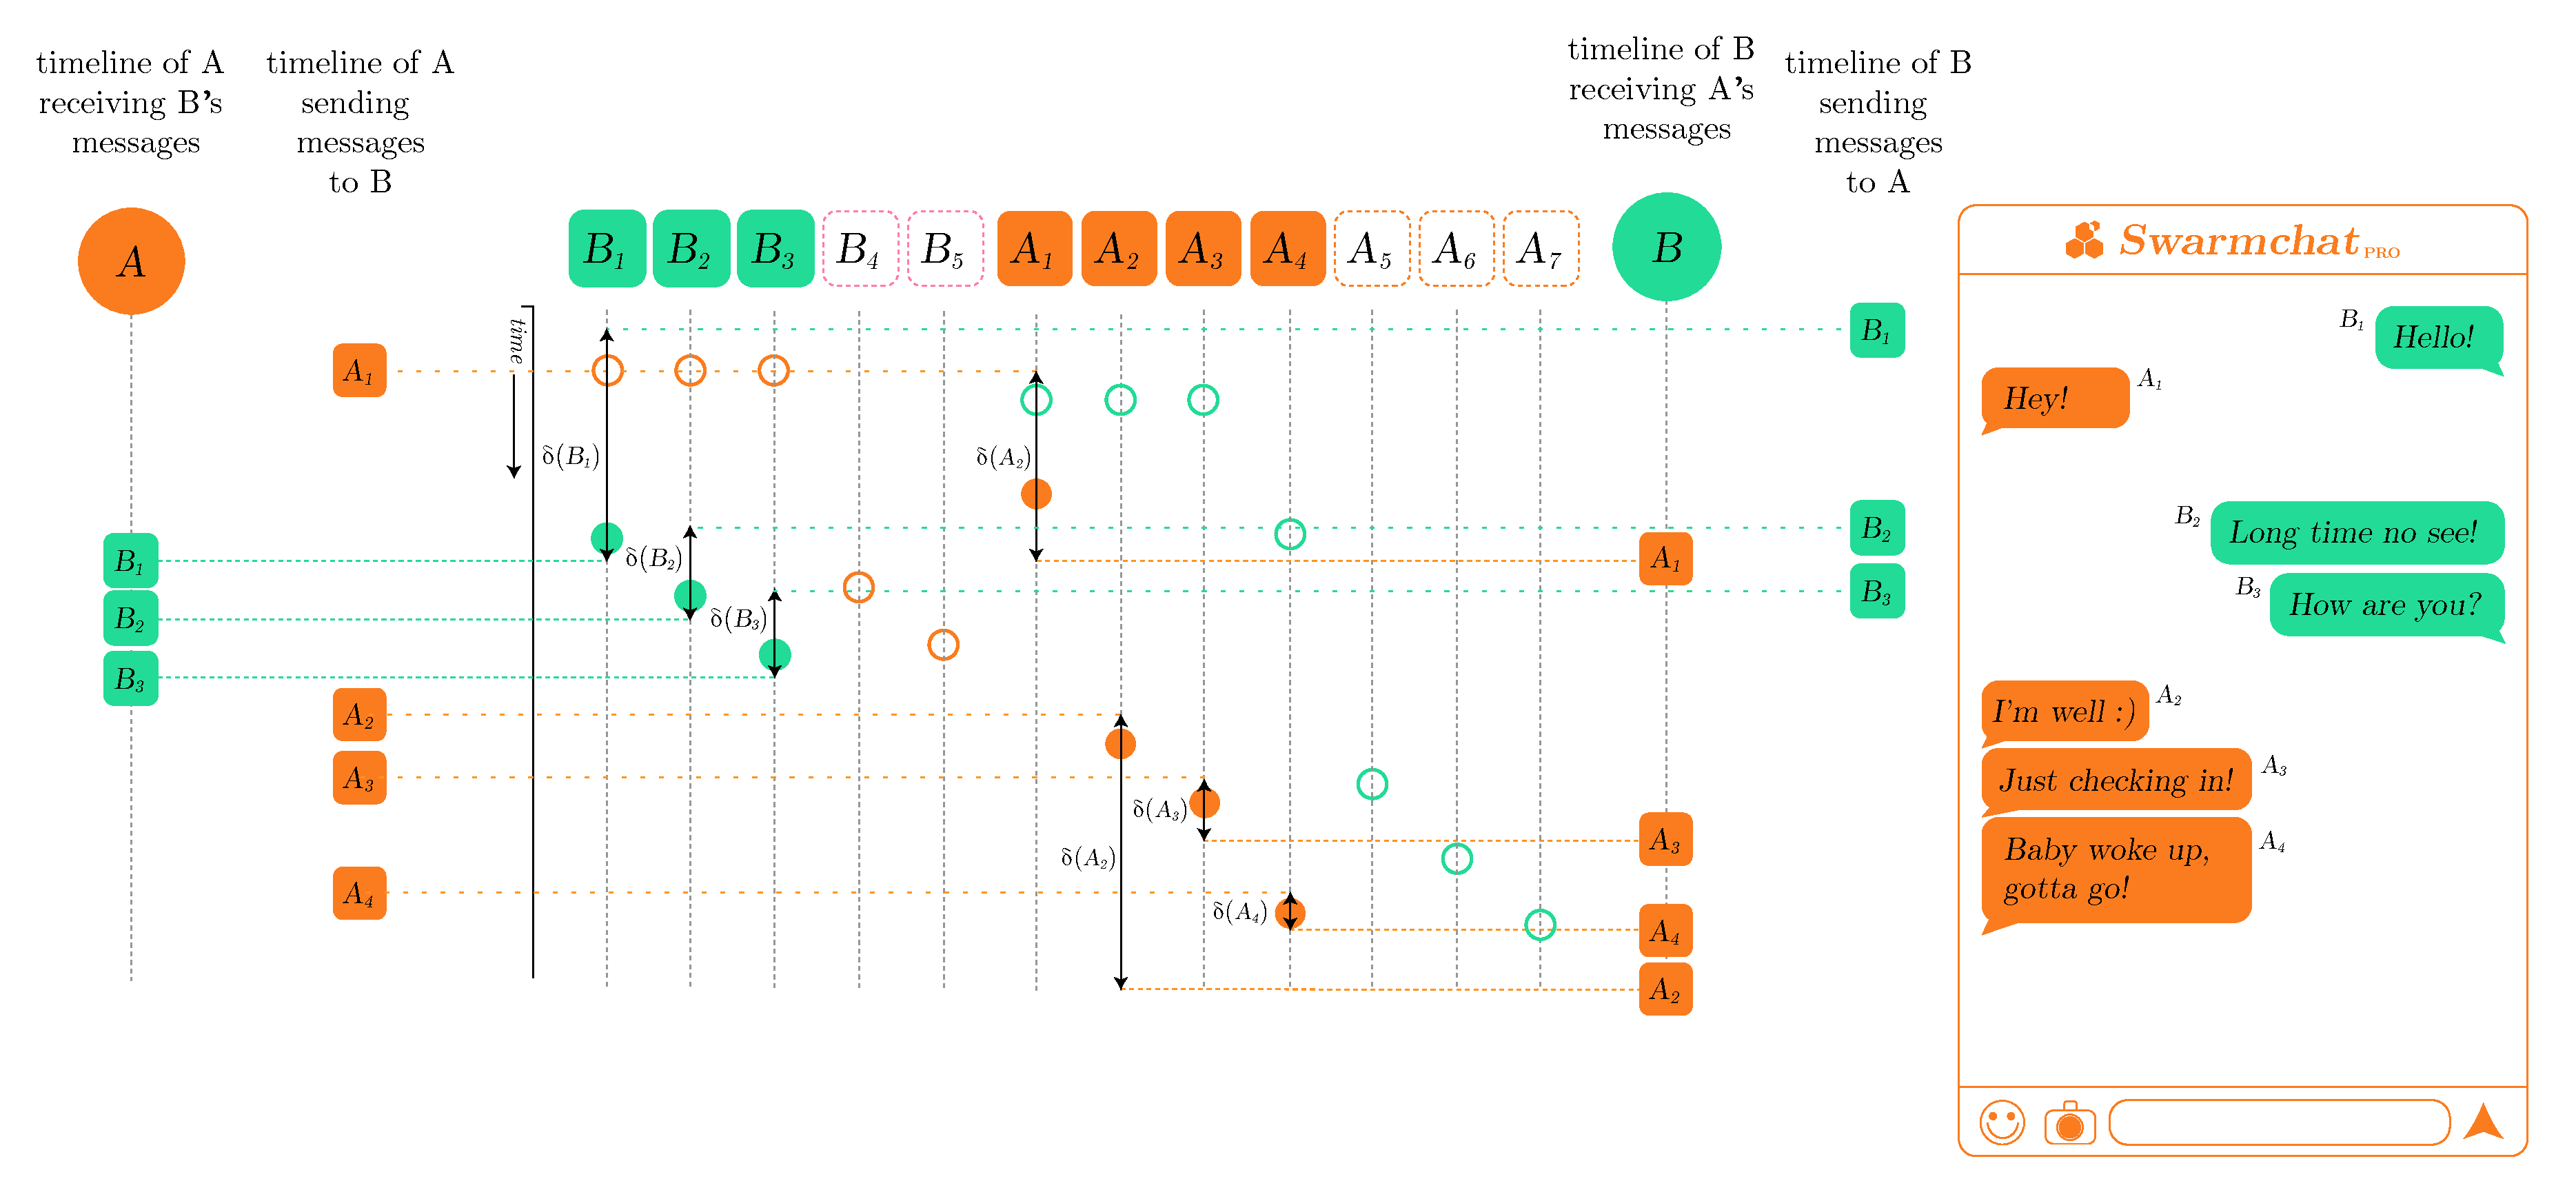
\includegraphics[width=\textwidth]{fig/outbox-feed-latency.pdf}  
\centering
\caption[Advance requests for future updates \statusgreen]{Advance requests for future updates. The diagram shows the time of a series of events during instant messaging between two parties A and B using outbox feeds. The columns designate the neighbourhood locations of the feed update addresses. Circles show the time of protocol messages arriving: colors indicate the origin of data, empty circles are retrieve requests, full circles are push sync deliveries arriving at the respective neighbourhood. Note that the outbox addresses are deterministic 3 messages ahead so retrieve requests can be sent before the update arrives.

Importantly, latency between one party sending a message $m$ and the other receiving it is shown as $\delta(m)$. Messages $A_3$ and $A_4$ arrive before $A_2$ which can be reported and repaired. If address predictability was only possible for 1 message ahead, both $B_2$ and $B_3$ would have much longer latencies.

Also note that the latency of $B_2$ and $B_3$ are helped by advance requests:  the retrieve requests for $B_4$ and $B_5$ are sent upon receipt of $B_1$ and $B_2$ and arrive at their neighbourhood the same time as the messages $B_2$ and $B_3$ arrive at theirs, respectively. If address predictability was only 1 message ahead, this would also cause both $B_2$ and $B_3$ to have much longer latencies.}
\label{fig:outbox-feed-latency}
\end{figure}


\subsubsection{Post-compromise security}

A key management solution called \gloss{double ratchet} is the de-facto industry standard used for encryption in instant messaging.
It is customary to use the \gloss{extended triple Diffie--Hellmann key exchange} (\gloss{X3DH}) to establish the initial parameters for the double-ratchet key chains (see \ref{sec:pss-key-exchange}).

Double-ratchet combines a ratchet based on a continuous key-agreement protocol with a ratchet based on key-derivation function \cite{perrin2016double}. This scheme can be generalised \cite{alwen2019double} and understood as a combination of well-understood primitives and shown to provide  (1) forward secrecy, (2) backward secrecy,%
%
\footnote{Also known as future secrecy or post-compromise security.}
%
and (3) immediate decryption and message loss resilience.


\begin{figure}[htbp]
\centering
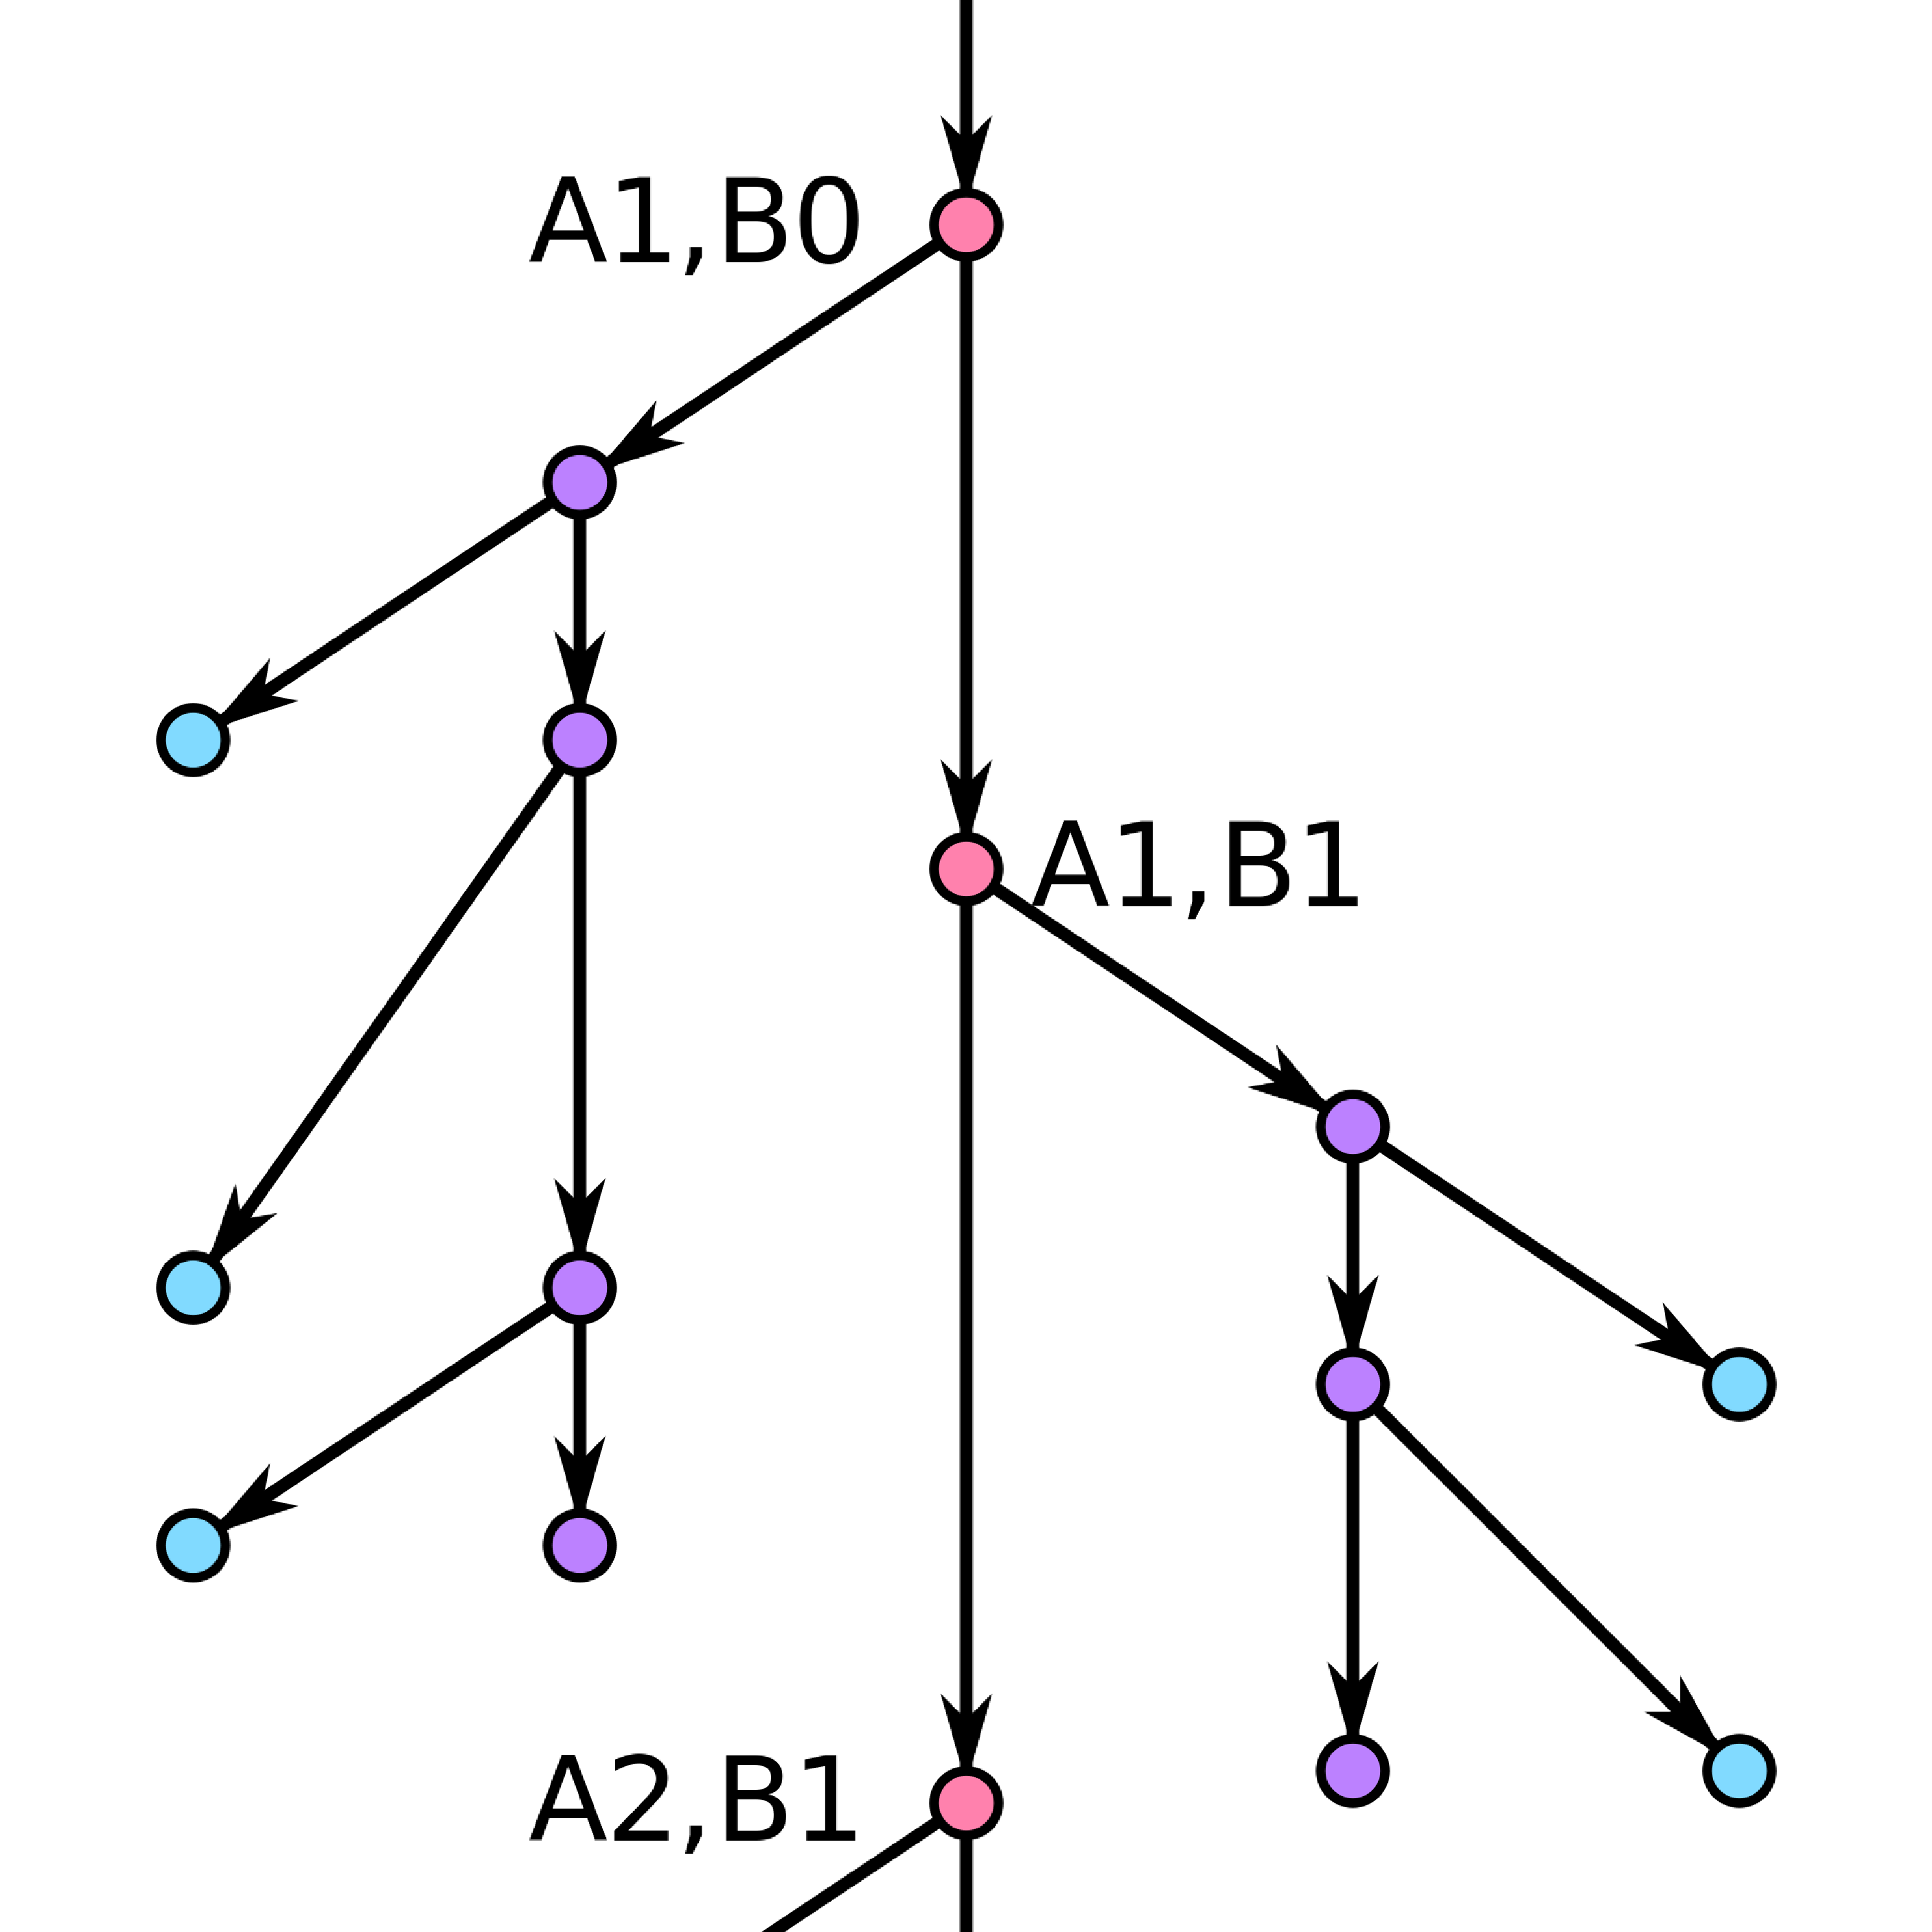
\includegraphics[width=.6\textwidth]{fig/double-ratchet.png}
\caption[Future secrecy for update addresses \statusorange]{Future secrecy for update addresses}
\label{fig:double-ratchet-for-feeds}
\end{figure}

On top of the confidentiality due end-to-end encryption, Swarm offers further resistance to attacks. Due to forwarding Kademlia, the sender is ambiguous and deniable. Due to normal push-sync and pull-sync traffic, messages are also obfuscated. To make it really hard for an attacker, the sequence of indexes can also provide \gloss{future secrecy} if we add more key chains to the double-ratchet machinery. Beside root, sending and receiving encryption key chains, we would need to introduce two more: outgoing and incoming \gloss{outbox index key chains}, see figure \ref{fig:double-ratchet-for-feeds}. As a result of this measure the underlying communication channel is obfuscated, i.e. intercepting an outbox update chunk and knowing its index, reveals nothing about previous or subsequent outbox update indexes. This makes subsequent messages prohibitively difficult and costly to monitor or intercept.

In \ref{sec:feed-integrity}, we used factoring in the payload hash into the indexing scheme to achieve non-mergeability of chains (unambiguous history). Inspired by this, we propose also to factor in the payload hash into the subsequent feed update index. This results in the additional property called \gloss{recover security},  which, intuitively, ensures that once an adversary manages to forge a message from A to B, then no future message from A to B will be accepted by B.
This is guaranteed if the authenticity of A's  messages to B affects the subsequent \gloss{feed index}. If there is a mismatch (one of the messages was forged), messages will be looked up at the wrong address and therefore the communication channel will be abandoned and a new one is initiated. Such a communication channel represents a completely confidential zero-leak solution for real-time messaging.




\section{Pss: direct push messaging with mailboxing \statusgreen}\label{sec:pss}

\green{}

This section introduces \emph{pss}, Swarm's direct node-to-node push messaging solution. 
Functionalities of and motivation for its existence are playfully captured by alternative resolutions of the term:

\begin{itemize}
\item \emph{postal service on Swarm} -- Delivering messages if recipient is online or depositing for download if not.
\item \emph{pss is bzz whispered} -- Beyond the association to Chinese whispers, it surely carries the spirit and aspiration of Ethereum Whisper.%
%
\footnote{Whisper is a gossip-based dark messaging system, which is no longer developed. It never saw wide adoption due to its (obvious) lack of scalability. Whisper, alongside Swarm and the Ethereum blockchain, was the communication component of the holy trinity, the basis for Ethereum's original vision of web3.}
%
Pss piggy-backs on Swarm's \gloss{distributed storage} for chunks and hence inherits their full incentivisation for relaying and persistence. At the same time it borrows from Whisper's crypto, envelope structure and API.
\item \emph{pss! instruction to hush/whisper} -- Evokes an effort to not disclose information to 3rd parties, which is found exactly in the tagline for pss: truly zero-leak messaging where beside anonymity and confidentiality, the very act of messaging is also undetectable.
\item  \emph{pub/sub system} -- API allows publishing and subscription to a topic.
\end{itemize}

First, in \ref{sec:trojan}, we introduce Trojan Chunks, i.e. messages to storers that masquerade as chunks whose content address happens to fall in the proximity of their intended recipient. 
\ref{sec:pss-key-exchange} discusses the use of pss to send a contact message to open a real time communication channel.
In \ref{sec:addressed-envelopes}, we explore the mining of feed identifiers to target a neighbourhood with the address of a single owner chunk and present the construct of an addressed envelope. Finally, building on Trojan chunks and addressed envelopes, \ref{sec:notification-requests} introduces update notification requests.
The user experience pss offers is discussed later in \ref{sec:pss-ux}. 

\subsection{Trojan chunks\statusgreen}\label{sec:trojan}

Cutting edge systems promising private messaging often struggle to offer truly zero-leak communication \cite{kwon2016riffle}. While linking the sender and recipient is cryptographically proven to be impossible, resistance to traffic analysis is harder to achieve. Having sufficiently large anonymity sets requires high volumes available at all times. In the absence of mass adoption, guaranteeing high message rate in dedicated messaging networks necessitates constant fake traffic. With Swarm, the opportunity arises to disguise messages as chunk traffic and thereby obfuscate even the act of messaging itself. 

We define a \gloss{Trojan chunk} as a content addressed chunk the content of which has a fixed internal structure, see figure \ref{fig:trojan-chunk}:

\begin{enumerate}
    \item \emph{span} -- 8 byte little endian uint64 representation of the length of the message  
    \item \emph{nonce} -- 32 byte arbitrary nonce 
    \item \emph{Trojan message} -- 4064 byte asymmetrically encrypted message ciphertext with underlying plaintext composed of
    \begin{enumerate}
        \item \emph{length} -- 2 byte little endian encoding of the length of the message in bytes $0\leq l\leq 4030$,
        \item \emph{topic} -- $32$ byte obfuscated topic id   
        \item \emph{payload} -- $m$ bytes of a message 
        \item \emph{padding} -- $4030-m$ random bytes.
    \end{enumerate}
\end{enumerate}

\begin{figure}[htbp]
\centering
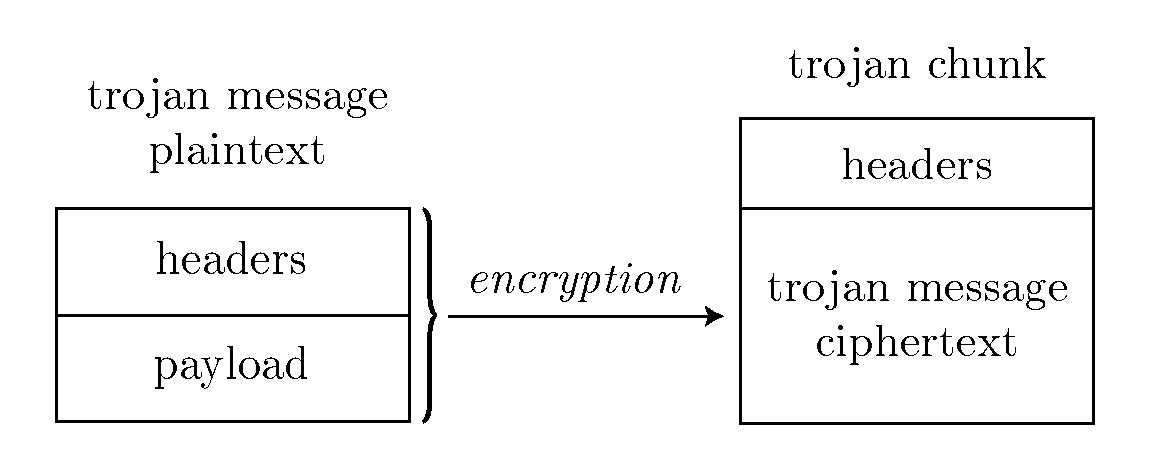
\includegraphics[width=\textwidth]{fig/trojan-generic.pdf}
\caption[Trojan chunk or pss message\statusgreen]{A pss message is a Trojan chunk that wraps an obfuscated topic identifier with a Trojan message, which in turn wraps the actual message payload to be interpreted by the application that handles it.}
\label{fig:trojan-generic}
\end{figure}

\begin{figure}[htbp]
\centering
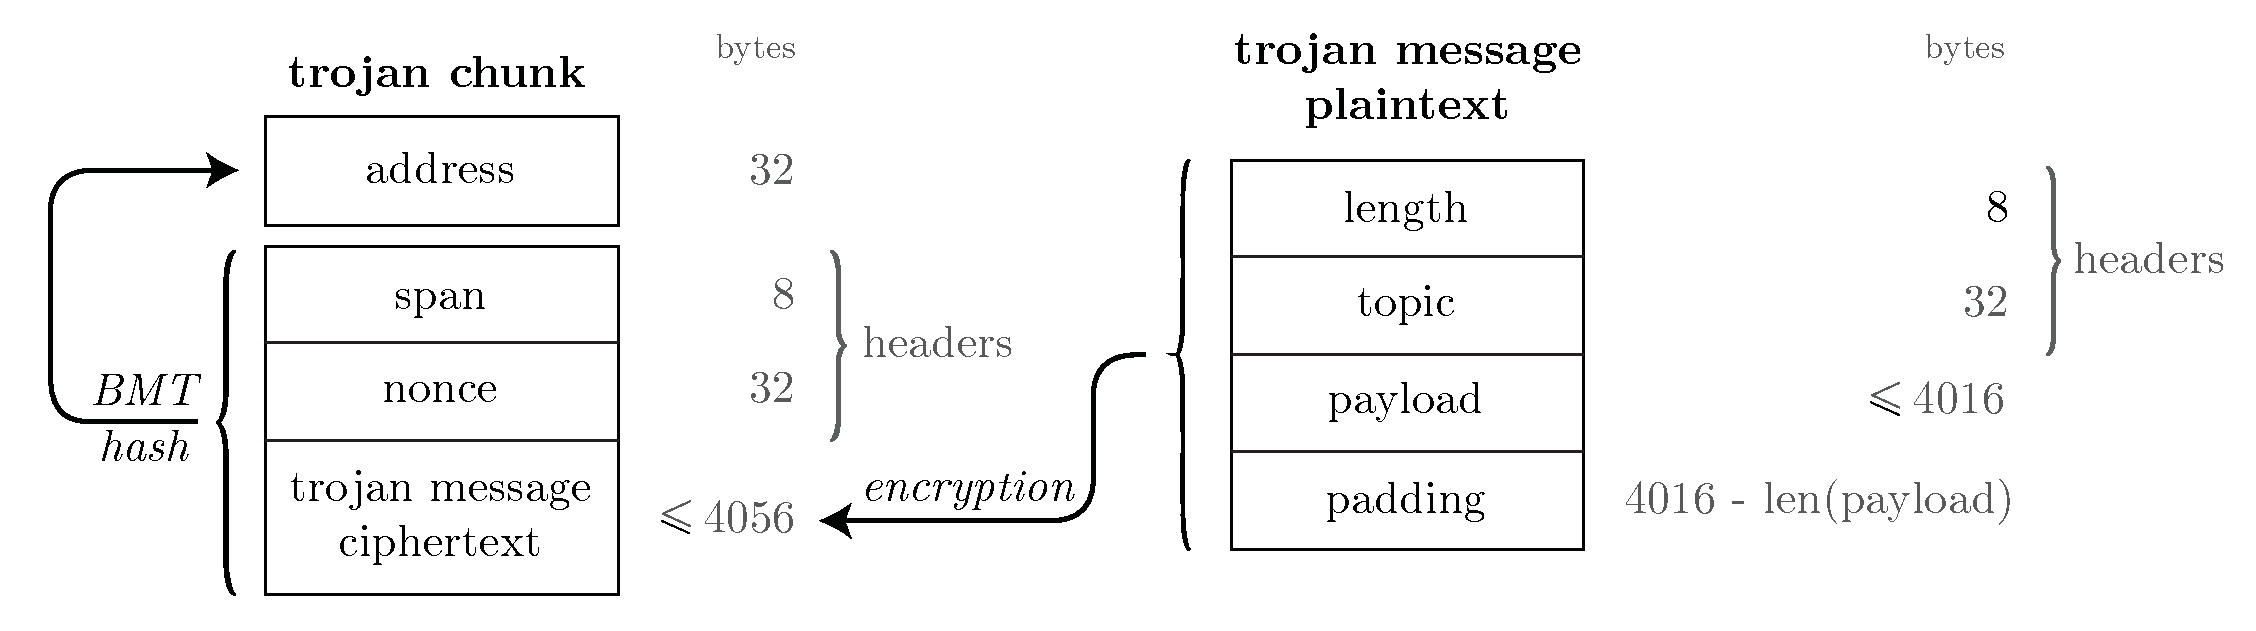
\includegraphics[width=\textwidth]{fig/trojan-chunk-3.pdf}
\caption[Trojan chunk\statusgreen]{The Trojan chunk wraps an asymmetrically encrypted Trojan message.}
\label{fig:trojan-chunk}
\end{figure}

Knowing the public key of the recipient, the sender wraps the message in a trojan message (i.e. prefixing it with length, then padding it to 4030 bytes) then encrypts it using the recipient's public key to obtain the ciphertext payload of the trojan chunk by asymmetric encryption. Then the sender finds a random nonce such that when it is prepended to the payload, the chunk hashes to an address that starts with a \gloss{destination target} prefix. The destination target is a bit sequence that represents a specific neighbourhood in the address space. If the target is a partial address derived as a prefix of the recipient overlay address, matching the target means that the chunk falls in the neighbourhood of the recipient. If only the public key is known, it is assumed that it is the bzz account of the recipient, i.e. their overlay address can be calculated from it%
%
\footnote{Alternative overlays can be associated with a public key, and several public keys can be listened on by a node at a particular address.}
%
(see \ref{sec:overlay-addressing} and \ref{spec:format:bzzaddress}). The sender then uploads the resulting chunk to Swarm with postage stamps of their choice which then ends up being synced to the recipient address' neighbourhood. If the recipient node is online they receive the chunk for certain provided the bit length of the matching target is greater than the recipient's neighbourhood depth. In practice, targets should be $n+c$ bits long where $n$ is the estimated average depth in swarm and $c$ is a small integer. 

\subsubsection{Receiving Trojan messages}

The recipient only knows that a chunk is a pss message if and when they successfully opened the Trojan message with the private key corresponding to the public key that they advertise as their resident key (see \ref{sec:pss-key-exchange}) and do an integrity check/topic matching. Nodes that want to receive such Trojan Messages will keep trying to open all messages that they are closest to. Forwarding nodes (or anyone else apart from sender and recipient) have no way to distinguish between a random encrypted chunk and a trojan message, which means that communication is perfectly obfuscated as generic chunk traffic.

After the recipient has opened the envelope using asymmetric decryption, there is a combined step of integrity check and topic matching. Knowing the length of the payload (from the first 2 bytes of the message), the recipient takes the payload slice and calculates the Keccak256 hash of it. Now for each topic the client has a subscription to, it then hashes the payload hash together with the topic. If the resulting segment xor-ed with the topic matches the obfuscated topic id in the message then the message is indeed meant as a message with the said topic and the registered handler is called with the payload as argument.

\subsubsection{Mailboxing for asynchronous delivery}

If the recipient is not online the chunk will prevail as any other chunk would, depending on the postage stamp it has. Whenever the recipient node comes online, it pull-syncs the chunks from the neighbourhood closest to it, amongst them all the Trojan chunks, and amongst them their own as yet unreceived messages. In other words, through Trojan messages pss automatically provides asynchronous \emph{mailboxing} functionality, i.e. 
without any further action needed from the sender, even if they are offline at the time that their correspondent has sent them, undelivered messages are preserved and available to the recipient whenever they come online. The duration of mailboxing is controlled with postage stamps in exactly the same way as the storage of chunks, in fact, it is totally indistinguishable.

\subsubsection{Mining for proximity}

The process of finding a hash close to the recipient address is analogous to mining blocks on the blockchain. The nonce segment in a Trojan chunk also plays exactly the same role as a block nonce: it provides sufficient entropy to guarantee a solution. The difficulty of mining corresponds to the length of the destination target: The minimum proximity order required to ensure that the recipient will receive the message needs to be higher than the neighbourhood depth of the recipient%
%
\footnote{It makes sense to use the postage lottery batch depth (see \ref{sec:postage-lottery}) as a heuristic for the target proximity order when mining a Trojan chunk. This is available as a read-only call to the postage stamp smart contract.}
%
when it comes online, so it is logarithmic in the number of nodes in the network. The expected number of nonces that need to be tried per Trojan message before an appropriate content address is found is exponential in the difficulty, and therefore equal to the number of nodes in the network. As the expected number of computational cycles needed to find the nonce equals the network size, in practice, mining a Trojan will never be prohibitively expensive or slow even for a single node. A small delay in the second range is expected only in a network of a billion nodes and even that is acceptable given that Trojan messages are meant to be used only for one-off instances such as initiations of a channel. All subsequent real-time exchange will happen using the previously described bidirectional outbox model using single owner chunks.


\subsubsection{Anonymous mailbox}

Asynchronous access to pss messages is guaranteed if the postage stamp has not yet expired. The receiver only needs to create a node with an overlay address corresponding to the destination target advertised to be the recipient's resident address.    

One can simply create an anonymous mailbox. An anonymous mailbox can receive pss messages on behalf of a client and then publish those on a separate, private feed so that the intended recipient can read them whenever they come back online.

\subsubsection{Register for aggregate indexing}

As mentioned in \ref{sec:indexing-schemes}, aggregate indexing services help nodes in monitoring sporadic feeds. For instance, a forum indexer aggregates the contribution feeds of registered members. For public forums, off-chain registration is also possible and can be achieved by simply sending a pss message to the aggregator. 


\subsection{Initial contact for key exchange\statusgreen}\label{sec:pss-key-exchange}


Encrypted communication requires a handshake to agree on the initial parameters that are used as inputs to a symmetric key generation scheme. The \gloss{extended triple Diffie--Hellmann key exchange} (\gloss{X3DH}) is one such protocol \cite{marlinspike2016x3dh} and is used to establish the initial parameters for a post-handshake communication protocol such as the \emph{double-ratchet scheme} discussed earlier in the section on feeds (see \ref{sec:feed-as-channel}). 
In what follows, we describe how the X3DH protocol can be implemented with pss in a serverless setting. 

Swarm's X3DH uses the same primitives as are customary in Ethereum, i.e. secp256k elliptic curve, Keccak256 hash, and a 64-byte encoding for EC public keys. 

The Swarm X3DH protocol is set out to allow two parties to establish a shared secret that forms the input used to determine the encryption keys which will be used during post-handshake two-way messaging. The \emph{initiator} is the party that initiates a two-way communication with the \emph{responder}. The responder is supposed to advertise the information necessary for parties not previously known to the responder to be able to initiate contact. Zero leak communication can be achieved by first performing an X3DH to establish the seed keys used by the double-ratchet protocol for the encryption of data, as well as the feed indexing methodology used. This will enable the responder to retrieve the updates of the outbox feed.

X3DH uses the following keys:%
%
\footnote{The protocol specifies one-time pre-keys for the responder, but these can be safely ignored since they only serve as replay protection, which is solved by other means in this implementation.}

\begin{itemize}
\item responder long-term public identity key - $K^{\mathrm{ENS}}_r$,
\item responder resident key (aka signed pre-key) - $K^{\mathrm{Res}}_r$,
\item initiator long-term identity key - $K^{\mathrm{ID}}_i$,
\item initiator ephemeral key for the conversation - $K^{\mathrm{EPH}}_i$.
\end{itemize}{}



\begin{figure}[htbp]
   \centering
   \includegraphics[width=\textwidth]{fig/prekey-bundle-feed-update.pdf}
   \caption[X3DH pre-key bundle feed update \statusgreen]{The X3DH pre-key bundle feed update contains the resident key and resident address and is optionally together encrypted with the ENS name hash to prove uniqueness and provide authentication.}
\label{fig:prekey-bundle-feed-update}
\end{figure}


A \gloss{pre-key bundle} consists of all information the initiator needs to know about responder. However, instead of being stored on (usually 3rd-party) servers, this information is instead stored in Swarm. For human-friendly identity management, ENS can be optionally used to provide familiar username based identities. The owner of the ENS resolver represents the long-term public identity key of this persona and is considered authenticated. The long-term identity address can be used to construct an epoch-based feed with a topic id indicating it provides the pre-key bundle for would be correspondents. When communication is initiated with a new identity, the latest update from the feed is retrieved by the initiator, containing the current \emph{resident key} (aka \emph{signed pre-key}) and current \emph{addresses of residence}, i.e. (potentially multiple) overlay destination targets where the persona is expecting she may receive pss messages. The signature in the feed update chunk signs both the resident key (cf. signed pre-key) and the destination targets. The public key that is recovered from this signature gives the long-term identity public key, see figure \ref{fig:prekey-bundle-feed-update}.


\begin{figure}[htbp]
   \centering
   \includegraphics[width=.8\textwidth]{fig/x3dh-initial-message.pdf}
   \caption[X3DH initial message \statusgreen]{X3DH initial message. Initiator retrieves the ENS owner as well as the latest update of responder's pre-key bundle feed containing the resident key and resident address. Initiator sends their identity key and an ephemeral key to responder's resident address using the resident key for encryption. }
\label{fig:x3dh-initial-message}
\end{figure}


In order to invite a responder to an outbox-feed based private communication channel, the initiator first looks up the responder's public pre-key bundle feed and sends an initial message to the responder (see figure \ref{fig:x3dh-initial-message}) in which the intent to communicate is indicated. She then shares the parameters required to initiate the encrypted conversation. This consists of the public key of its long-term identity, as well as the public key of the ephemeral key-pair which has been generated just for that conversation. These details are delivered to the potential responder by sending a Trojan pss message addressed to the responder's current address of residence which is also being advertised in their pre-key bundle feed. 

\begin{figure}[htbp]
   \centering
   \includegraphics[width=.6\textwidth]{fig/x3dh.pdf}
   \caption[X3DH secret key \statusgreen]{X3DH secret key. Both parties can calculate the triple Diffie-Hellmann keys and xor them to get the X3DH shared secret key used as the seed for the post-handshake protocol.}
   \label{fig:x3dh}
\end{figure}

After the responder receives this information, both parties have all the ingredients needed to generate the triple Diffie-Hellmann shared secret, see figure \ref{fig:x3dh}.%
%
\footnote{If the X3DH does not use one-time pre-keys, the initial message can in theory be re-sent by a third party and lead the responder to assume genuine repeated requests. Protocol replay attacks like this are eliminated if the post-handshake protocol adds random key material coming from the responder. 
But the initial Trojan message can also be required to contain a unique identifier, e.g. the nonce used for mining the chunk. Reusing the id is not possible since it leads to the same chunk.}
%
This shared secret constitutes the seed key for the double-ratchet continuous key agreement protocol as used in the signal protocol. The double-ratchet scheme provides forward secrecy and post-compromise security to the end-to-end encryption. By applying separate key-chains for the outbox feed's indexing scheme, additional \gloss{recover security}, i.e. resilience to message insertion attack, can be achieved. Most importantly, however, by adding forward and backward secrecy to outbox addresses, the communication channel is obfuscated, which renders sequential message interception contingent on the same security assumptions as encryption and therefore eliminates the only known attack surface for double-ratchet encryption. The obfuscation and deniability of the channel based on outbox feeds, together with the initial X3DH message being disguised indistingushable as a chunk warrants designating this as  zero-leak communication.

\subsection{Addressed envelopes\statusgreen}\label{sec:addressed-envelopes}

\subsubsection{Mining single owner chunk addresses}

The question immediately arises whether it makes sense to somehow mine single owner chunks. Since the address in this case is the hash of a 32 byte identifier and a 20 byte account address, the id provides sufficient entropy to mine addresses even if the owner account is fixed. So for a particular account, if we find an id such that the resulting single owner chunk address is close to a target overlay address, the chunk can be used as a message in a similar way to Trojan chunks. Importantly, however, since the address can be mined before the chunk content is associated with it, this construct can serve as an \gloss{addressed envelope}.

Let us make explicit the roles relevant to this construct:

\begin{itemize}
\item \emph{issuer} ($I$) - creates the envelope by mining an address. 
\item \emph{poster} ($P$) - puts the content into the envelope and posts it as a valid single owner chunk to Swarm.
\item \emph{owner} ($O$) - possesses the private key to the account part of the address and can thus sign off on the association of the payload to the identifier. This effectively decides on the contents of the envelope.
\item \emph{target} ($T$) - the constraint for mining: a bit sequence that must form the prefix of the mined address. It represents a neighbourhood in the overlay address space where the envelope will be sent. The length of the target sequence corresponds to the difficulty for mining. The longer this target is, the smaller the neighbourhood that the envelope will be able to reach.
\item \emph{recipient} ($R$) - the party whose overlay address has the target sequence as its prefix and therefore the destination of the message
\end{itemize}

The envelope can be perceived as open: since the poster is also the owner of the response single owner chunk, they are able to control what content is put into the chunk. By constructing such an envelope, the issuer effectively allows the poster to send an arbitrary message to the target without the computation requirement needed to mine the chunk. See figure \ref{fig:addressed-envelope-events}. 


\begin{figure}[htbp]
   \centering
   \includegraphics[width=0.75\textwidth]{fig/prepaid-addressed-envelopes-events.pdf}
   \caption[Stamped addressed envelopes timeline of events \statusgreen]{Stamped addressed envelopes timeline of events. Issuer $I$ creates the envelope encrypted for $P$ with an identifier such that $P$ as the single owner of the chunk, produces an address that falls in the recipient $R$'s neighbourhood. As a result (only) $P$ can fill the envelope with arbitrary content and then use simple push-syncing to post it to $R$.}
   \label{fig:addressed-envelope-events}
\end{figure}

All the poster needs to do when they wish to send a message to the recipient is to create a Trojan message and sign it against the identifier using the private key of the same account the issuer used as an input when they mined the address. If they do this, the chunk will be valid. See figure \ref{fig:addressed-envelope}.


\begin{figure}[htbp]
   \centering
   \includegraphics[width=\textwidth]{fig/addressed-envelope.pdf}
   \caption[Stamped addressed envelopes \statusgreen]{A stamped addressed envelope issued for $P$ and addressed to $R$ consists of an identifier which is mined so that when used to create a single owner chunk owned by $P$, it produces an address which falls within $R$'s neighbourhood. This allows $P$ to construct a message, sign it against the identifier and using the postage stamp, post it using the network's normal push-syncing to $R$ for free. }
   \label{fig:addressed-envelope}
\end{figure}

\subsubsection{Pre-paid postage}

These chunks behave in the same way as normal Trojan messages, with their privacy properties being the same if not somewhat better since the issuer/recipient can associate a random public key with which the message is encrypted, or even use symmetric encryption. If a postage stamp is pre-paid for an address and given to someone to post later, they can use push-sync to send the chunk to the target without the poster needing to pay anything, the cost of this having already been covered by the \gloss{stamped addressed envelope}. Such a construct effectively implements \emph{addressed envelopes with pre-paid postage} and serves as a base layer solution for various high-level communication needs: 1) push notifications about an update to subscribers without any computational or financial postage burden on the sender 2) free contact vouchers 3) zero-delay direct message response.  


\subsubsection{Issuing a stamped addressed envelope}

Issuing a stamped addressed envelope involves the following process:

\begin{enumerate}
\item \emph{assume} issuer $I$, prospective poster $P$, and prospective recipient $R$ with public keys $K_I, K_P, K_R$ and overlay addresses $A_I, A_P, A_R$.
\item \emph{mine} -- $I$ finds a nonce $N_R$ such that when used as an identifier to create a \gloss{single owner chunk}, the  address of the chunk hashes to $H_R$ which is in the nearest neighbourhood of $A_R$.
\item \emph{pay postage} -- $I$ signs $H_R$ to produce a witness for an appropriate postage payment to produce stamp $PS_R$.
\item \emph{encapsulate} -- package $N_R$ and $PS_R$ which represent the pre-paid envelope pre-addressed to recipient address and encrypt it with $K_P$ then wrap it as a Trojan chunk.
\item \emph{mine} -- find a nonce $N_P$ such that the Trojan chunk hashes to $H_P$ which is in the nearest neighbourhood of $A_P$. 
\end{enumerate}




\subsubsection{Receiving a stamped addressed envelope}

A prospective poster $P$ is assumed to receive a a Trojan message consisting of pre-paid envelope $E$. In order to open it, she carries out the following steps:

\begin{enumerate}
    \item \emph{decrypt} message with the private key belonging to $K_P$
    \item \emph{deserialise} unpack and identify $PS_R$ and $N_R$, extract $H_R$ from $PS_R$
    \item \emph{verify} postage stamp $PS_R$ and check if $N_R$ hashed with the account for $K_P$ results in $H_R$ to ensure the associated address is in fact owned by $P$.
    \item \emph{store} $N_R$ and $PS_R$ 
\end{enumerate}

\subsubsection{Posting a stamped addressed envelope}

When the poster wants to use the envelope to send an arbitrary message $M$ to $R$ (with recipient $R$ potentially unknown to the sender), they must follow the following steps:

\begin{enumerate}
\item \emph{encrypt} the message content $M$ with $K_R$ to create a payload and wrap it in Trojan message $T$
\item \emph{hash} the encrypted Trojan message resulting in $H_T$
\item \emph{sign} $H_T$ against the identifier $N_R$ using the private key belonging to $K_P$ producing signature $W$
\item \emph{encapsulate} nonce $N_R$ as id, the signature $W$ and the Trojan message $T$ as the payload of a valid single owner chunk with address $H_R$
\item \emph{post} the chunk with the valid stamp $PS_R$
\end{enumerate}

\subsubsection{Receiving a posted addressed envelope}

When $R$ receives chunk with address $H_R$

\begin{enumerate}
\item \emph{verify} postage stamp $PS_R$ and validate the chunk as a single owner chunk with payload $T$.
\item \emph{decrypt} $T$ with the private key belonging to $K_R$.
\item \emph{deserialise} the plaintext as a Trojan message, identify the message payload $M$ and check its integrity.
\item \emph{consume} $M$.
\end{enumerate}

\subsection{Notification requests\statusgreen}\label{sec:notification-requests} 

\yellow{new}

This section elaborates on the concept of addressed envelopes and presents three flavours, each implementing different types of notifications.

\subsubsection{Direct notification from publisher}

If an issuer wants a recipient to be notified of the next activity on a feed, she must construct a stamped addressed envelope embedded in a regular Trojan message and send it to the publisher, see figure \ref{fig:direct-notification}. If the issuer is also the recipient, then the account that is used in the request and the one in the response envelope may be one and the same. 


When the feed owner publishes an update to her feed, the reference to the update chunk is put into the envelope and is sent to the recipient. More formally, the publisher creates a single owner chunk from the identifier representing the pre-addressed envelope and therefore, as the owner, signs off on the identifier associated with the feed update content as the payload of the single owner chunk. Right after this, the same publisher acting as the poster, push-syncs the chunk to the swarm. This construct is called \gloss{direct notification from publisher}. 

\begin{figure}[htbp]
   \centering
   \includegraphics[width=\textwidth]{fig/direct-notification.pdf}
   \caption[Direct notification request and response \statusgreen]{A direct notification request contains a reference to a feed and wraps a pre-paid envelope mined for $P$ (the publisher or a known distributor of the feed) and addressed to recipient $R$. The response is identical to the process used for generic stamped addressed envelopes and only differs in that the message is supposed to be the feed update or a reference to its content.}
   \label{fig:direct-notification}
\end{figure}

The Trojan message specifies in its topic that it is a notification and is encrypted using the public key. As the address is mined to match the recipient overlay address on a sufficiently long prefix, the message ends up push-synced to the recipient's neighbourhood. Whenever the recipient comes online and receives the chunk by push-sync it detects that it is intended as a message. It can be identified as such either by decrypting the chunk content successfully with the key for the address they had advertised, or in case that the recipient has issued the pre-addressed envelope themselves, simply by looking it up the against the record of the address they saved when it was issued.  See figure \ref{fig:direct-notification-events} for the timeline of events.


\begin{figure}[htbp]
   \centering
    \includegraphics[width=0.8\textwidth]{fig/direct-notification-events.pdf}
   \caption[Direct notification from publisher timeline of events \statusgreen]{Direct notification from publisher timeline of events. Issuer $I$ constructs a prepaid envelope for the publisher or a known distributor of the feed $P/F$ and addressed to recipient $R$. Together with a feed topic $I$, it is sent to $P/F$ wrapped in a pss trojan message. $P/F$ receives it and stores the request. When they publish the update, they wrap it in the envelope, i.e. sign the identifier received from $I$ against the feed update notification message and post it as a chunk, which $R$ will receive and hence, be notified of the feed update. }
   \label{fig:direct-notification-events}
\end{figure}


Notifications coming from publishers directly enable the poster to put arbitrary content into the envelope. The poster is at the same time the owner so that they can sign off on any content against the identifier when posting the envelope. In order for the issuer to be able to create the notification chunk address in advance, the prospective poster's account must be known. However, the feed update address need not be fixed, so this scheme remains applicable to (sporadic) epoch-based feeds.

\subsubsection{Notification from neighbourhood}

Assume there is a feed whose owner has not revealed their overlay (destination target) or refuses to handle notifications.  The feed is updated sporadically using simple sequential indexing and therefore polling is not feasible when it comes to looking up the latest update, especially as the consumer can go offline any time.
Is there a way for consumers to still get notified? 

We introduce another construct, a \gloss{neighbourhood notification} which works without the issuer of the notification knowing the identity of prospective posters. It presupposes, however, that the content or at least the hash of the content is known in advance so that it can be signed by the issuer themselves.


An issuer wants a recipient to be notified of the next update. The issuer can create a \gloss{neighbourhood notification} request, simply a Trojan chunk wrapping a message. This message contains an addressed envelope (identifier, signature and postage stamp) that the poster can use to construct the single owner chunk serving as the notification. Note that the notification message need not contain any new information, merely the fact of receiving it is sufficiently informative to the recipient. In order to indicate what it is a notification of, the notifications payload contains the feed update address. Upon receiving the notification, the receiver can then simply send a regular retrieve request to fetch the actual feed update chunk containing or pointing to the content of the message. See figure \ref{fig:notification-from-neighbourhood} for the structure of neighbourhood notifications and notification requests.
                                

\begin{figure}[htbp]
\centering
\includegraphics[width=\textwidth]{fig/notification-from-neighbourhood.pdf}
\caption[Neighbourhood notifications \statusgreen]{Neighbourhood notification requests are not only including identifier and postage stamp but also a notification message together with the signature attesting it against the address. Thus $P$ needs to construct the actual notification and when publisher $F$ posts their update to $P$-s neighbour, $P$ can post the notification to recipient $R$.}
\label{fig:notification-from-neighbourhood}
\end{figure}

If the notification needs only to contain the feed update address as its payload then associating it with the identifier can be signed off by the issuers themselves. This signature together with the identifier should be considered a necessary component of the envelope and must be sent as part of the notification request.
Unlike the \emph{open} envelopes used with publishers directly, neighbourhood notifications can be viewed as \emph{closed} envelopes, where the content is sanctioned by the issuer in advance. 

Now the issuer and not the poster becomes the owner of the chunk and the signature is already available to the poster when they create and post the notification. As a consequence no public key or account address information is needed from the poster. In fact, the identity of the poster does not need to be fixed, any peer could qualify as a candidate poster. Issuers therefore can send the notification request to the neighbourhood of the feed update chunk. The nearest neighbours will keep holding the request chunk as dictated by the attached postage stamps until they receive the appropriate feed update chunk that indicates the receipt of the notification. See figure \ref{fig:neighbourhood-notification-events} for the timeline of events when using neighbourhood notifications.

\begin{figure}[htbp]
\centering
\includegraphics[width=0.8\textwidth]{fig/neighbourhood-notification-events.pdf}
\caption[Neighbourhood notification timeline of events \statusgreen]{Neighbourhood notification timeline of events. Issuer $I$ mines an identifier for a single owner chunk with themselves as owner such that the chunk address falls in recipient $R$'s neighbourhood. The issuer, being the owner also must sign the identifier against a prefabricated reminder and remember which node should be notified. When $P$ syncs the feed update the notification is sent to $R$, delivered by the usual push-syncing.}
\label{fig:neighbourhood-notification-events}
\end{figure}
  

But how can we make sure that notifications are not sent too early or too late? While the integrity of notification chunks is guaranteed by the issuer as their single owner, measures must also be taken to prevent nodes that manage the notifications from sending them before the update should actually arrive. It would be ideal if the notification could not be posted before the arrival of the update, otherwise false alarms could be generated by malicious nodes that service the request.

A simple measure is to encrypt the message in the request  message symmetrically with a key that is only revealed to the prospective poster when they receive the feed update, for instance, the hash of the feed update identifier.
In order to reveal that the notification request needs to be matched on arrival of the feed update, the topic must be left unencrypted, so here we do not encrypt the pss envelope asymmetrically but only the message and symmetrically.

Note that the feed update address as well as identifier can be known if the feed is public, so neighbourhood notifications are to be used with feeds whose subsequent identifiers are not publicly known.

\subsubsection{Targeted chunk delivery}

Normally, in Swarm's DISC model, chunks are requested with retrieve requests, which are forwarded towards the neighbourhood designated by the requested chunk address (see \ref{sec:retrieval}). The first node on the route that has the chunk will respond with it and the chunk is delivered as a backwarded response travelling back along the same route that the request has taken. In certain cases, however, it may be useful to have a mechanism to request a chunk from an arbitrary neighbourhood where it is known to be stored and send it to an arbitrary neighbourhood where it is known to be needed. A construct called \gloss{targeted chunk delivery} is meant for such a use case: the request is a Trojan pss message while the response, the delivery, must be a single owner chunk wrapping the requested chunk, with an address mined to fall into the neighbourhood of the recipient.  


\begin{figure}[htbp]
\centering
\includegraphics[width=\textwidth]{fig/targeted-chunk-delivery.pdf}      
\caption[Targeted chunk deliveries \statusgreen]{Targeted chunk deliveries are similar to neighbourhood notifications in that they are not only pre-addressed and pre-paid but also pre-signed. Similarly, the identifier is mined so that given issuer $I$ as the owner, it produces an chunk address that falls in recipient $R$'s neighbourhood. Here the issuer signs the identifier against the hash of a content addressed chunk that they want to see posted to $R$. If the targeted chunk delivery request lands with any node that has the chunk in question, they can use the envelope and the content of the chunk to produce a valid response which is a single owner chunk wrapping a content addressed chunk.}
\label{fig:targeted-chunk-delivery}
\end{figure}

\begin{figure}[htbp]
\centering
\includegraphics[width=.8\textwidth]{fig/targeted-chunk-delivery-events.pdf}
\caption[Targeted chunk delivery timeline of events\statusgreen]{Targeted chunk delivery timeline of events. Uploader $U$ uploads a chunk to Swarm and it lands with a storer node $S$. Nodes within $P$ replicate (and pin) this chunk. Now, if issuer $I$ wants this chunk delivered to $R$, it will take the prepaid envelope addressed to $R$ and sends it to the neighbourhood of a known host unencrypted so that anyone who has the chunk can construct the notification and send or store it for later.}
\label{fig:targeted-chunk-delivery-events}
\end{figure}



These 'chunk-in-a-soc' responses are structurally similarly to neighbourhood notifications in that the payload's hash is already known (the content address of the chunk requested). The requestor can then sign off on its association with the identifier which, along with the signature, is sent as part of the request, see figure \ref{fig:targeted-chunk-delivery-events}. A node that got the request only needs to have the requested chunk stored and they can construct the response as a valid single owner chunk addressed to the recipient's neighbourhood.
This makes the request generic, i.e. not fixed to the identity of the prospective poster. Therefore it can be sent to any neighbourhood that requires the content. Even multiple requests can be sent simultaneously: due to the uniqueness of the valid response, multiple responses cannot hurt chunk integrity (see \ref{sec:single-owner-chunks} and \ref{sec:feed-integrity}). Targeted delivery is used in missing chunk recovery, see \ref{sec:recovery-chunks}.

The difference is that neighbourhood notifications are not giving any new information while targeted chunk delivery supplies the chunk data. Also, a chunk delivery wrapped in a single owner chunk uses no message wrapping and has no topic. Neither request nor response uses encryption.
A consequence of not using encryption is that, if there are alternative sources, mining the initial Trojan request has the constraint that the address matches any target. 

Table \ref{tab:notifications} summarises various properties of the three notification-like constructs.

\begin{table}[htpb]
    \centering
    \begin{tabular}{c|c|c|c|c|}
    type & owner & poster & request encryption & notification  \\\hline
         direct & poster & publisher & asymmetric on pss & feed update  content\\
         neighbourhood & issuer & any & symmetric on envelope & feed update arrival\\
         targeted delivery & issuer & any & none & chunk content\\
    \end{tabular}
    \caption[Feed update notifications]{Requests of and responses to types of feed update notifications and targeted chunk delivery.}
    \label{tab:notifications}
\end{table}

\chapter{Persistence \statusgreen}\label{sec:persistence}


In this chapter we focus on data persistence, i.e. the ways of making sure that content stays available on Swarm. 
We introduce error coding schemes, which can provide a way to secure availability against churn at a cost of the storage overhead. 
In particular \glossplural{erasure code} (\ref{sec:repair}) and \glossplural{entanglement code}  %(\ref{sec:entanglements}) 
provide redundancy optimised for documents with different access patterns.
% First we discuss how popular content stays alive due to opportunistic caching (\ref{sec:caching}).  
After introducing the notion of local pinning in \ref{sec:reupload}, i.e. the ability to mark content as sticky in your Swarm local storage, we will present ways in which this can help achieve global persistence across the network. We define a \gloss{missing chunk notification protocol}, which allows content maintainers to make sure their published content is restored in the event of some chunks being garbage collected, by proxying retrieval through select \glossplural{pinner} of the content.

Finally, in \ref{sec:insurance}, we present the holy grail, that is, decentralised file insurance: combining the concepts of the postage lottery and missing chunk notifications, Swarm offers a protocol that enables users to pay other nodes to keep their content available. While ordinary storer nodes are rewarded for storing chunks via the postage lottery, for a higher premium, staked nodes will promise to take responsibility for storing and responding to requests for chunks, accepting the risk of punitive measures that will be imposed on them in the event that the insured data does not remain available to the network.


\section{Redundancy, latency and repair \statusgreen}\label{sec:repair}

\green{}

\subsection{Error correcting codes \statusgreen}\label{sec:error-correcting-codes}

Error correction codes are commonly used to ensure that data remains available even if parts of the storage system become faulty. In particular, they allow us to construct storage schemes (data encoding and distribution) that solve this problem more efficiently than simple replication. The problem is framed in the context of guaranteeing a certain probability that the data will be retrievable given a model expressing the expected fault conditions in the storage subsystems.

Coding theory in general is often applied to \glossplural{RAID} and computer hardware architecture synchronising arrays of disks to provide resilient data-centre storage.
\glossupperplural{erasure code} in particular see the problem as: how does one encode stored data into shards distributed across $n$ disks so that the entirety of the data remains fully retrievable in the face of a particular probability that one disk becomes faulty.
Similarly, in the context of a distributed chunk store, the problem can be reformulated as the question: how does one encode the stored data into chunks distributed across nodes in the network so that the entirety of the data remains retrievable in the face of a particular probability that one chunk is found to be missing.%
%
\footnote{The distributed chunk store model uses fixed-sized chunks which can only be either completely lost or completely undamaged. Since the Swarm content storage uses the hashes of chunks as their addresses, and since the chunks are stored by custodian nodes that are randomly distributed in the same address space, we are safe to assume that a particular storage allocation is independent of all the other nodes and data. This assures that recovering a chunk at any point can practically be thought of as potentially failing with equal and independent probability.}

There are various parameters one can optimise on, principally: storage and bandwidth overhead. Erasure codes are theoretically optimal to minimise storage overhead, but require retrieving large amount of data for a local repair.
Entanglement codes, on the other hand, require a minimal bandwidth overhead for a local repair, but at the cost of storage overhead that is in multiples of 100\%. 

\subsection{Redundancy by erasure codes \statusgreen}\label{sec:erasure}


The \gloss{Cauchy-Reed-Solomon erasure code} (henceforth \gloss{CRS}, \cite{lubyetal1995CRS}, \cite{plank2006optimizing}) is a \emph{systemic} \gloss{erasure code} which, when applied to a data blob of $m$ fixed-size chunks, produces $k$ extra chunks (so called \emph{parity chunks}) of the same size in such a way that any $m$ out of $n=m+k$ fix-sized chunks are enough to reconstruct the original blob. The storage overhead is therefore given by $\frac{k}{m}$.%
%
\footnote{%
There are several open source libraries that implement Reed Solomon or Cauchy-Reed-Solomon coding. See \cite{plank2009performance} for a thorough comparison.}

Both the encoding and the decoding of CRS codes takes $O(mk)$ time, where $m$ is the number of data chunks, $k$ is the number of additional chunks as well as the maximum number of chunks that can be lost without losing decodeability. If $k$ is defined as a given fraction of $m$ which is necessary for guaranteeing a certain probability of retrievability under the condition of a fixed probability $p$ of losing a single chunk, the time complexity of CRS codes becomes $O(n^2)$, which is unacceptable for large files. 

\subsection{Per-level erasure coding in the Swarm chunk tree \statusgreen}

Swarm uses a hierarchical Merkle tree \cite{merkle1980protocols} to reorganise data into fixed sized chunks which are then sent off to the Swarm nodes to store.
Let $h$ be the byte length of the hash used, and let $b$ be the branching factor. Each vertex represents the root hash of a subtree or, at the last level, the hash of a $b\cdot h$ long span (one chunk) of the document. Generically we may think of each chunk as consisting of $b$ hashes.


\begin{figure}[htbp]
   \centering
   \input{fig/chunk.tex}
   \caption[Swarm chunk \statusgreen]{A Swarm chunk consists of 4096 bytes of the file or a sequence of 128 subtree hashes.}
   \label{fig:chunk}
\end{figure}


\begin{figure}[htbp]
   \centering
   \input{fig/Swarm-hash-basic.tex}
   \caption[A generic node in the tree has 128 children \statusgreen]{A generic node in the tree has 128 children.}
   \label{fig:Swarm-hash-basic}
\end{figure}

During normal Swarm lookups, a Swarm client performs a lookup for a hash value and receives a chunk in return. This chunk in turn constitutes another $b$ hashes to be looked up and retrieve another $b$ chunks and so on until the chunks received belong to the actual document (see figure \ref{fig:Swarm-hash-split}).


\begin{figure}[htbp]
   \centering
   \input{fig/Swarm-hash-split.tex}
   \caption[Swarm hash split \statusgreen]{The Swarm tree is the data structure encoding how a document is split into chunks.}
   \label{fig:Swarm-hash-split}
\end{figure}

While off-the-shelf erasure coding could be used for documents uploaded into Swarm, this solution has immediate problems. Apart from the quadratic complexity of encoding, \gloss{chunking} the CRS-encoded data blob with the BMT chunker would result in certain chunks being more vulnerable, since their retrieval is dependent on the retrieval of the chunks that encode all their ancestor nodes in the chunk tree.

This prompted us to try and align the notion of Swarm chunk with the chunk used in the CRS scheme which led us to encode redundancy directly into the Swarm tree. This is achieved by applying the \emph{CRS scheme} to each set of chunks that are children of a node in the Swarm tree.

The \emph{chunker} algorithm incorporating CRS encoding works in the following way when splitting the document:

\begin{enumerate}
\item Set the input to be the data blob.
\item Read the input one chunk (say fixed 4096 bytes) at a time. Count the chunks by incrementing a counter $i$. 
\item Repeat step 2 until either there's no more data (note: the last chunk read may be shorter) or $i \equiv 0$ mod $m$.
\item Use the CRS scheme on the last $i \mod m$ chunks to produce $k$ parity chunks resulting in a total of $n \leq m+k$ chunks.
\item Calculate the hashes of all these chunks and concatenate them to result in the next chunk (of size $i\mod m$ of the next level. Record this chunk as next.
\item If there is more data repeat 2. 
\item If there is no more data but the next level data blob has more than one chunk, set the input to this and repeat from 2.
\item Otherwise record the blob to be the root chunk.
\end{enumerate}

% Fixing the branching factor of the Swarm hash as $n=128$ and $h=32$ as the size of the \emph{SHA3 Keccak hash} gives us a chunk size of $4096$ bytes.

% We start splitting the input data into chunks, and after each $m$ chunks add $k=n-m$ parity check chunks using a Reed-Solomon code so that now any $m\text{-out-of-}n$ chunks are
% sufficient to reconstruct the document. On the next level up the chunks are composed of the hashes of the $m$  data chunks and the $k$ hashes of the parity chunks. Let's take the first $m$
% of these and add an additional $k$ parity chunks to those such that any $m$ of the resulting $n$
% chunks are sufficient to reconstruct the origial $m$ chunks. And so on and on every level. In terms of
% availability, every subtree is equally important to every other subtree at this level. The resulting
% data structure is not a balanced tree since on every level $i$ the last $k$ chunks are parity leaf
% chunks while the first $m$ are branching nodes encoding a subtree of depth $i-1$ redundantly.
A typical piece of our tree would look like this (see figure \ref{fig:Swarm-hash-erasure}).


\begin{figure}[htbp]
   \centering
   \resizebox{1\textwidth}{!}{
        \input{fig/Swarm-hash-erasure.tex}
   }
   \caption[Swarm hash erasure \statusgreen]{The Swarm tree with extra parity chunks using $112$ out of 128 CRS encoding. Chunks $p_{0}$ through $p_{15}$ are parity data for chunks $H_0 $ through $H_{111}$ on every level of intermediate chunks.}
   \label{fig:Swarm-hash-erasure}
\end{figure}


This pattern repeats itself all the way down the tree. Thus hashes $H_{m+1}$ through $H_{127}$ point to parity data for chunks pointed to by $H_0$ through $H_{m}$. Parity chunks $P_i$ do not have children and so the tree structure does not have uniform depth.

\subsubsection{Incomplete batches}

If the number of file chunks is not divisible by $m$, we cannot proceed with the last batch in the same way as the others. We propose that we encode the remaining chunks with an erasure code that guarantees at least the same level of security as the others. Note that this is not as simple as choosing the same redundancy. For example a $50\text{-out-of-}100$ encoding is much more secure against loss than a $1\text{-out-of-}2$ encoding even though the redundancy is $100\%$ in both cases. Overcompensating, we still require the same number of parity chunks even when there are fewer than $m$ data chunks.

This leaves us with only one corner case: it is not possible to use our $m\text{-out-of-}n$ scheme on a single chunk ($m=1$) because it would amount to $k+1$ copies of the same chunk. The problem is that any number of copies of the same chunk all have the same hash and therefore are automatically deduplicated. Whenever a single chunk is left over ($m=1$) (this is always the case for the root chunk itself), we replicate the chunk as the payload of one of more single owner chunk with an address that is deterministically derivable from the content owners public key and the original root hash, thus enabling us to provide an arbitrary level redundancy for storage of data of any length.

\subsubsection{Upper limit of retrieval latencies}

When downloading a file with erasure coding, data subsumed under an intermediate chunk can be recovered having any $m$ out of $m+k$ children. A downloader can initiate requests for all $m+k$ and will need to wait only for the first $m$ to be delivered in order to proceed.
This technique can effectively shield unavailability of chunks due to occasional faults like network contention, connectivity gaps, and node churn; prohibitively overpriced neighbourhoods or even malicious attacks targeting certain localities. Given a particular fault model for churn and throughput, erasure codes can be calibrated to
\emph{guarantee an upper limit on retrieval latencies}, a strong service quality proposition.





\section{Pinning, reupload and missing chunk notifications \statusyellow}\label{sec:reupload}

This section introduces the notion of pinning, i.e. locally sticky content protected from the garbage collection routines of its storage nodes (\ref{sec:pinning}). In \ref{sec:global-pinning}, we discuss how pinners of content can play together to pin content for the entire network globally. \ref{sec:repair} defines a recovery protocol that downloaders can use to notify storers of missing chunks belonging to content they are responsible for pinning globally. With such on-demand repair and the uninterrupted download experience it enables, recovery implements a poor man's persistence measure which can ensure network wide availability of specific chunks without requiring the financial outlay of insurance.

\subsection{Local pinning \statusgreen}\label{sec:pinning}

Local \gloss{pinning} is the mechanism that makes content sticky and prevents it from being garbage collected. It pins the content only in the node's local storage to enable local persistence of data and speedy retrieval. Pinning is applied at the chunk level in the local database of the client and exposes an API for users to pin and unpin files and collections in their local node (see \ref{sec:features} and \ref{spec:api:pinning}).

In order to pin all the chunks comprising files, the clients need to keep a \gloss{reference count} for each chunk which incremented and decremented when the chunk is pinned and unpinned respectively. As long as the reference count is non-zero, the chunk is considered to be part of at least one document that is pinned and therefore immune to garbage collection. Once a chunk is pinned, only when the reference count returns to zero, after it has been respectively unpinned for every time it has been pinned, is the chunk once again considered for garbage collection.

Local pinning can be thought of as a feature which allows Swarm users to mark specific files and collections as important, and therefore not removable. Pinning a file in local storage will also make it always accessible for the local node even without an internet connection. As a result using pinned content for storage of local application data enables an offline-first application paradigm, with Swarm automatically handling network activity on re-connection. However, since if the chunk is not in the node's area of responsibility, local pinning by itself is not enough to ensure the chunk generally retrievable to other nodes, since the pinner is not in the Kademlia neighbourhood where the chunk is meant to be stored and hence where it will be searched for when the chunk is requested using the pull-sync protocol. In order to provide this functionality, we must implement a second half of the pinning protocol.

\subsection{Global pinning}\label{sec:global-pinning}

If a chunk is removed as a result of garbage collection by storers in its nominated neighbourhood , local pinning in nodes elsewhere in the network will offer no way to retrieve it alone. In order for pinning to aid global network persistence, two issues must be tackled:

\begin{itemize}
    \item  notify global pinners of a missing chunk belonging to the content they pin -- so they can re-upload it,
    \item  maintain retrievability of chunks that are garbage collected but globally pinned -- so that downloaders experience no interruption. 
\end{itemize}

One naive way to achieve this is to periodically check for a pinned chunk in the network and re-upload the contents if it is not found. This involves a lot of superfluous retrieval attempts, has immense bandwidth overhead and ultimately provides no reduction in latency.

An alternative, reactive way is to organise notifications to the pinner which are somehow triggered when a user accesses the pinned content and finds a chunk to be unavailable. Ideally, the downloader notifies the pinner with a message that triggers (1) the re-upload of the missing chunk, and (2) the delivery of the chunk in response to the request of the downloader.  

\subsubsection{Fallback to a gateway}

Let us assume that a set of pinner nodes have the content locally pinned and our task is to allow fallback to these nodes. In the simplest scenario, we can set up the node as a gateway (potentially load-balancing to a set of multiple pinner nodes): Users learn of this gateway if it is included in the manifest entry for the file or collection. If the user is unable to download the file or collection from the Swarm due to a missing chunk, they can simply resort to the gateway and find all chunks locally.
This solution benefits from simplicity and therefore likely the first global persistence milestone to be implemented.  

\subsubsection{Mining chunks to pinners' neighbourhoods}

The second, brute force solution is more sophisticated in that the publisher can construct the chunks of a file in such a way that they all fall within the neighbourhood of the pinner (or of any pinner node in the set). In order to do this, the publisher needs to find an encryption key for each chunk of the file so that the encrypted chunk's address matches one of the pinners on at least their first $d$ bits, where $d$ is chosen to be comfortably larger than that pinner's likely neighbourhood depth.%
%
\footnote{Note that in case that the pinner nodes do not share infrastructure and the mined chunks need to be sent to pinners with the push-sync protocol, then each postage batch used will be used at most $n$ times. Although this non-uniformity implies a higher unit price, if pinners pin out of altruism (i.e. not for compensation), only a minimum postage price needs to be paid.
}

These solutions can already accomplish persistence, but they reintroduce a degree of centralisation and also require publishers to maintain and control server infrastructure. Surely, they also suffer from the usual drawbacks of server-client architecture, namely decreased fault-tolerance and the likelihood of compromised performance due to the fact that requests will be more concentrated. These solutions also do not address the question of how pinner nodes are provided the content and disregard any privacy considerations. For these reasons, although the low-level pinning API is provided for swarm users, usage of it is considered to be a less desirable alternative to the gold standard of incentivised file insurance discussed elsewhere. As such use cases should be carefully considered to ensure that they would not benefit from the enhanced privacy and resilience provided by the incentivised system.



\subsection{Recovery \statusyellow}\label{sec:recovery-chunks}


In what follows we describe a simple protocol for notifying pinners of the loss of a chunk, which they can react to by (1) re-uploading the lost chunk to the network and at the same time (2) responding to the notifier by delivering to them the missing chunk. The procedures relating to the missing chunk notification protocol are specified in detail in  \ref{spec:format:recovery} while related data structures are formalised in \ref{spec:format:recovery}.

If replicas of a chunk are distributed among willing hosts (pinners), then downloaders not finding a chunk can fall back to a \gloss{recovery} process requesting it from one of these hosts using the \gloss{missing chunk notification protocol} called \gloss{prod}.
As usual, the resolutions of this acronym capture the properties of the protocol:

\begin{itemize}
\item \emph{protocol for recovery on deletion} - A protocol between requestor and pinners to orchestrate chunk recovery after garbage collection. The process is triggered by downloaders if they fail to retrieve a chunk.
\item \emph{process request of downloader} - Recovery hosts continuously listen for potential recovery requests from downloaders.
\item \emph{provide repair of DISC} - 
Prod provides a service to repair the Swarm DISC, in the event of data loss.
\item \emph{pin and re-upload of data} -     
Hosts pin the data and re-upload it to its designated area when prompted with a recovery request. 
\item \emph{prompt response on demand}  - If the requestor demands a prompt direct response, the host will post the missing chunk using a recovery response envelope and accompanying postage stamp.
\end{itemize}

\subsubsection{Recovery hosts}

\glossupperplural{recovery host} are pinners that are willing to provide pinned chunks in the context of recovery. These pinners are supposed to have indicated that they will take on this task to the publisher and to have downloaded all the relevant chunks and have pinned them all in their local instance. 

The publisher that wishes to advertise its publication as globally pinned or repairable would then gather the overlay addresses of these volunteering recovery hosts. In fact, it is sufficient to collect just the prefixes of the overlay with a length greater than Swarm's depth. We will call these partial addresses \gloss{recovery targets}.

Publishers will advertise the recovery targets for their content to the consumers of their data via a feed called a \gloss{recovery feed}. This feed can be tracked by consumers of the publisher's data based on the convention of constructing the topic using a simple sequential indexing scheme (see \ref{spec:format:recovery}). 

\begin{figure}[htbp]
\centering
\includegraphics[width=.8\textwidth]{fig/missing-chunk-notification.pdf} \caption[Missing chunk notification process \statusgreen]{The missing chunk notification process is similar to the targeted chunk delivery. Here a downloader mines the identifier to match their own address, i.e. a self-notification. If downloader $D$ encounters a missing chunk (a request times out), they send a recovery request to one of several neighbourhoods where there is a chance of finding the chunk. A successful response then will comprise a single owner chunk wrapping the missing chunk which is sent to the downloader. The chunk is also re-uploaded to the proper place in the network.}
\label{fig:missing-chunk-notification}
\end{figure}

\subsubsection{Recovery request}

Once the recovery hosts overlay targets are revealed to the downloader node, upon encountering a missing chunk, they should "prod" one of the recovery hosts by sending them a notification called a \gloss{recovery request}. This instance of targeted chunk delivery (see \ref{sec:notification-requests}) is a public unencrypted Trojan message containing at least the missing chunk address, see figure \ref{fig:recovery-request}.

\begin{figure}[htbp]
  \centering
  \includegraphics[width=\textwidth]{fig/recovery-request.pdf}
  \caption[Recovery request \statusgreen]{A recovery request is a Trojan chunk that is used as missing chunk notification. It is unencrypted and its payload is structured as a pss message containing the address of the chunk to be recovered. Optionally, it also includes a special recovery response envelope, an identifier with a signature attesting to the association of the identifier and the missing chunk hash.}
  \label{fig:recovery-request}
\end{figure}

In order to create a recovery request, a downloader needs to (1) create the payload of the message (2) find a nonce which when prepended to the payload results in a content address that matches one of the \gloss{recovery targets} indicated by the publisher. The matching target means that by push-syncing the chunk, it will be sent to the neighbourhood of the recovery host represented by a target prefix. 

If the targeted recovery host is online, they will receive the recovery request, extract the missing chunk address, retrieve the corresponding chunk that is pinned in their local storage and re-upload it to the network with a new postage stamp.

\subsubsection{Recovery response envelope}

A \gloss{recovery response envelope} serves to provide a way for recovery hosts to be able to respond directly to the originator of the recovery request, promptly and without associated cost or computational burden. It is an instance of targeted chunk delivery response (see \ref{sec:notification-requests}), an addressed envelope construct which is neutral to the poster but fixed for the content. The request message includes the components prospective posters will need to create the valid targeted chunk delivery response: an identifier with a signature attesting to the association of the identifier and the missing chunk hash. The identifier is chosen so that the address of the single owner chunk (the hash of the id with the owner account) falls into the requestor's neighbourhood and so it is automatically delivered there by the network's implementation of the push-sync protocol.

\begin{figure}[htbp]
\centering
\includegraphics[width=\textwidth]{fig/recovery-response-2.pdf}
\caption[Recovery response \statusgreen]{Recovery response is a single owner chunk that wraps the missing chunk. Anyone in possession of the headers and the chunk data is able to construct a valid single owner chunk and send it to the downloader for free.}
\label{fig:recovery-response}
\end{figure}

If the targeted recovery host is online, they will receive the recovery request and extract the missing chunk address as well as the identifier and the signature from the recovery response. After retrieving the corresponding chunk they pinned in their local storage they can simply create the recovery response. The hash of the identifier and the payload hash concatenated together forms the plain text of the signature. The signature received in the recovery request allows her to recover the public key of the requestor. From this public key they are able to calculate the requestor's address and finally, hashing this with the identifier results in the address of the single owner chunk. This scheme makes more sense if a postage stamp is also attached to the request which can be sent along with the recovery response as requestors are able to cover the Swap costs of returning the chunk which compensates the global pinner. In this way, it is possible for downloaders to intelligently cover the operating costs of nodes using micro-payments, hence ensuring the availability of data for the whole of the network.



\section{Insurance \statusorange}\label{sec:insurance}
 
\wip{still working on this}

\subsection{Insurance pool \statusorange}
We saw in \ref{sec:chunk-insurance} that the reward mechanism for postage lottery can also be used to facilitate and enforce insurance against lost data: where staked nodes take on the responsibility to store certain chunks staked against financial assets using the blockchain. 

Finally, we will discuss  1) how chunks are insured 2) how chunks travel across the network to the insurer 3) how later, any third party is able to audit the receipt for a chunk and, if it is found to be missing, initiate a process of litigation.

Let us imagine an insurance pool, a smart contract where registrants contribute stake. The pool represents nodes that, in return for a higher storage premium, stand to lose their stake if they lose a chunk. 

\subsection{Buying insurance on a chunk \statusred}

\subsection{Uploading with insurance \statusred}


\subsection{Accessing receipts \statusred}

The manifest entry for the insured file contains the reference to the data structure that maps insurer addresses to their public keys at the time of insuring the file. Once these pivots are known, any third party can calculate which insurer is responsible for each chunk. Once the insurer is known, one can look up their receipt store, the current receipt store root is easily found by simply looking up the insurer's receipt store feed.%
%
\footnote{In fact, it is not necessary to have the most up to date root, any state that is later than the start time of insurance should work.}
%
The actual receipt for the chunk can then be retrieved by traversing the receipt store using the original chunk address as the key. The insurer is implicitly responsible for insuring all the chunks of their receipt store as well as the receipt store feed. So if any chunk is found missing during this lookup procedure, the Merkle proof of segment that corresponds to the address of the missing chunk can be used to litigate. 
Otherwise, we can assume that the lookup is successful and the receipt is obtained by the user who can thus initiate litigation by submitting the receipt. 


\begin{figure}[htbp]
  \centering
  \caption[From retrieval to litigation \statusred]{From retrieval to litigation}
  \label{fig:flowchart-retrieval-litigation}
\end{figure}


Figure \ref{fig:flowchart-retrieval-litigation} gives a complete timeline of events starting from a third party user retrieving a file all the way to the file original insurer being punished.





\chapter{User experience}\label{sec:ux}

This chapter approaches Swarm features introduced in the previous chapters from the user's perspective. In \ref{sec:upload}, we discuss the user experience related to configuring uploads including aspects of postage, pinning, erasure coding, as well as tracking the progress of chunks propagating into the network with the help of upload tags. Then we turn to the user's experience of the storage API, uploading collections in \ref{sec:storage-ux} then turn to a description of the options available for communication in \ref{sec:messaging}. Finally, in \ref{sec:buzz-apiary}, we present a complete framework for web3 dapp development.

\section{Configuring and tracking uploads \statusgreen}\label{sec:upload}

\green{}

Upload is the most important interface for Swarm. Section \ref{sec:headers} presents the request headers (or alternatively, query parameters) used for configuring the upload APIs. In \ref{sec:tags} we introduce upload tags which can be used to track the state of the entire upload and displayed using progress bars together with an estimate of the expected time until the process will finish. Tags also record partial root hashes which can then be used to resume an upload in the eventuality it is interrupted before it is complete. In \ref{sec:postage-ux}, we sketch the scenarios relating to payment for upload and dispersal into the network, in particular how users can buy and attach stamps to chunks. Finally, \ref{sec:features} runs through optional parameters such as encryption, \gloss{pinning} and \glossplural{erasure code}.

\subsection{Upload options \statusgreen}\label{sec:headers}

The local http proxy offers the \lstinline{bzz} URL scheme as a storage API. The API is discussed further in \ref{sec:storage-ux} and formally specified in \ref{spec:api:storage}. Requests can specify Swarm specific options such as:

\begin{itemize}
\item \lstinline{tag} -- use this upload tag -- generated and returned in response header if not given. 
\item \lstinline{stamp} -- upload using this postage subscription -- if not given, the one used most recently is used. 
\item \lstinline{encryption} -- encrypt content if set, if set to a 64-byte hex value encoding a 256 bit integer, then that is used instead a randomly generated key. 
\item \lstinline{pin} -- pin all chunks of the upload if set. 
\item \lstinline{parities} -- apply CRS erasure coding to all intermediate chunks using this number of parities per child batch.
\end{itemize}

These options can be used as URL query parameters or specified as  headers. The name of the header is obtained by capitalising the parameter name and prefixing it with \lstinline{SWARM-},  i.e. \lstinline{SWARM-PARITIES}.  


\subsection{Upload tags and progress bar \statusgreen}\label{sec:tags}                                                                                        
When uploading a file or collection, it is useful to the user to know when the upload is complete in the sense that all newly created chunks are synced to the network and arrived at the neighbourhood where they can be retrieved. At this point, the uploader can "disappear", i.e. can quit their client. A publisher can disseminate the root hash and be assured, the file or collection is retrievable from every node on Swarm. 

Since the push-sync protocol provided statements of custody receipts for individual chunks we only need to collect and count those for an upload. Tracking the ratio of sent chunks and returned receipts provides the data to a \emph{progress bar}. An \gloss{upload tag} is an object representing an upload and tracking the progress by counting how many chunks have reached a particular state. The states are: 

\begin{itemize}
\item \emph{split} -- Number of chunks split; count chunk instances.
\item \emph{stored} -- Number of chunks stored locally; count chunk instances.
\item \emph{seen} -- Count of chunks previously stored (duplicates).
\item \emph{sent} -- Number of distinct chunks sent with push-sync.
\item \emph{synced} -- Number of distinct chunks for which the statement of custody arrived.
\end{itemize}

With the help of these counts, one can monitor progress of 1) chunking 2) storing 3) push-syncing, and 4) receipts.
If the upload tag is not specified in the header, one is randomly generated and is returned as a response header after the file is fully chunked. In order to monitor 1) and  2) during the upload, the tag needs to be created before the upload and supplied in the request header. Thus, the tag can be queried concurrently while the uploaded content is being processed. 

\subsubsection{Known vs unknown file sizes}

If the file size is known, the total number of chunks can be calculated, so that progress of chunking and storage can be meaningful from the beginning in proportion to the total.

If the size and total number of chunks split is not known prior to the upload, the progress of split is undefined. After the chunker has finished splitting, one can set the total count to the split count and from that point on, a percentage progress as well as ETA are available for the rest of the counts.

Note that if the upload also includes a manifest, the total count will serve only as an estimation until the total is set to the split count. This estimation converges to the correct value as the size of the file grows.


\subsubsection{Duplicate chunks}

\glossupperplural{duplicate chunk} are chunks that occur multiple times within an upload or across uploads. In order to have a locally verifiable definition, we define a chunk as a duplicate (or seen) if and only if it is already found in the local store.
When chunks enter the local store via upload they are push synced, therefore seen chunks need not be push-synced again.

In other words, only newly stored chunks need to be counted when assessing the estimated time of syncing an upload. If we want progress on sent and synced counts, they must report completeness in proportion to stored distinct chunks.

\subsubsection{Tags API} 

The http server's \lstinline{bzz} URL scheme provides the \lstinline{tags} endpoint for the tags API. It supports creating, listing and viewing individual tags. Most importantly there is an option to track the changes of a tag in real time using http streams. The tag API is specified in \ref{spec:api:tags}.



\subsection{Postage \statusgreen}\label{sec:postage-ux}

To impose a cost on uploads and efficiently allocate storage resources in the network, all uploads must be paid for.  This is somewhat unusual for the web, so a novel user experience needs to be developed. The closest and most familiar metaphor is a subscription.

\subsubsection{Postage subscriptions}

The user creates a subscription for a certain amount of time and storage (e.g. 1 month for 100 megabytes) and pays for it according to a price they learn from the client software (this is similar to how transaction fees are determined for the blockchain). Estimates for price can be read from the postage lottery contract. Subscriptions are named, but these names are only meaningful locally. The API will offer a few default options for the chosen storage period, on a logarithmic scale, e.g.: 

\begin{itemize}
\item \emph{minimal (a few hours)} -- Useful for immediate delivery of pss messages or single owner chunks part of ephemeral chat or other temporary files.
\item \emph{temporary (week)} -- Files or mailboxed messages meant not to be stored long but to be picked up by third parties asynchronously.
\item \emph{long term (year)} -- Default long term storage. 
\item \emph{forever (10 years)} -- Important content not to be lost/forgotten; to survive the growth of the network and subsequent increase of batch depth even if the uploader remains completely offline.
\end{itemize}

When the user uploads files, they can also indicate which subscription to use as the value of the \lstinline{stamp} upload parameter. If this is not given, the most recent one is used as default. If the size of the upload is known, the user can be warned if it is larger than the postage capacity. 

\subsubsection{Postage reuse strategies}

As mentioned in \ref{sec:postage-stamps}, encryption can be used to mine chunks to make sure they fall into \glossplural{collision slot} of postage batches. This strategy of mining chunks into batches makes sense for users that only want to upload a particular file/collection for a particular period or want to keep the option open to change the storage period for the file/collection independently of other uploads.

The alternative is to prepay a large set of postage batches and always keep a fixed number of them open for every period. This way we can make sure that we have a free \gloss{collision slot} in one of the batches for any chunk. The postage batches are ordered by time of purchase and when attaching a stamp to a chunk, the first batch is used that has a free slot for the chunk address in question. This more profitable strategy is used most effectively by power users including insurers who can afford to tie up liquidity for long time periods. The choice of strategy must be specified when creating a subscription.

\subsubsection{The postage subscription API}

In order to manage subscriptions, the \lstinline{bzz} URL-scheme provides the \lstinline{stamp} endpoint for the postage API (see \ref{spec:api:postage}). With this API the user can create postage subscriptions, list them, view them, top them up, or drain and expire them. 

When checking their subscription(s), the user is informed how much data has already been uploaded to that subscription and how long it can be stored given the current price (e.g. $88/100$ megabytes for $23$ days). If the estimated storage period is low, the files using the subscription are in danger of being garbage collected and therefore, to prevent that, topping up their subscription is instructive.


\subsection{Additional upload features \statusgreen}\label{sec:features}

Additional features such as swap costs, encryption, pinning and erasure coding can be set on upload using request headers. 


\subsubsection{Swap costs}

Uploading incurs swap costs coming from the push-sync protocol showing up in \gloss{SWAP} accounting (\ref{sec:accounting}). On every peer connection, if the balance tilts beyond the effective payment threshold, a cheque is to be issued and sent to the peer. If, however, the checkbook contract does not exist or is lacking sufficient funds to cover the outstanding debt, the peer connection is blocked. This may lead to unsaturated Kademlia and during that time, the node will count as a light node. The download can continue potentially using a smaller number of peers but, since some chunks will need to be sent to peers not closer to the request address than the node itself, the average cost of retrieving a chunk will be higher. 

It is useful to show this average number to the user as well as the average swap balance and the number of peer connections not available due to insufficient funds. This is accomplished through the SWAP API specified in \ref{spec:api:swap}.

\subsubsection{Encryption}

Encrypted upload is available by setting the upload option \lstinline{encryption} to a non-zero value. If the value is a hexadecimal representation of a 32 byte seed, that is used as a seed for encryption. Since encryption and decryption are handled by Swarm itself, it must only be used in situations where the transport between the http client and Swarm's proxy server can be guaranteed to be private. As such, this is not be used on public gateways, but only through local Swarm nodes or those that are private with well configured TLS and self-signed certificates.

\subsubsection{Pinning}

When uploading, the user can specify directly if they want the content to be pinned locally by setting the \lstinline{pin} upload option to a non-zero value. Beyond this, the local http server's \lstinline{bzz} URL scheme provides the \lstinline{pin} endpoint for the pinning API (see \ref{spec:api:pinning}). With this API, users can manage pinned content. A \lstinline{GET} request on the pinning endpoint gives a list of pinned files or connections.  The API also accepts \lstinline{PUT} and \lstinline{DELETE} requests on a hash (or domain name that resolves to a hash) to pin and unpin content, respectively.  

When pinning a file or collection, it is supposed to be retrieved and stored. Pinning triggers traversal of the hash tree and increments the reference count on each chunk; if a chunk is found missing locally, it is retrieved. After pinning, the root hash is saved locally. Unpinning triggers traversal of the hash and decrements the reference count of each chunk; if a chunk is found missing locally, it is ignored and a warning is included in the response. After unpinning, the hash is removed from the list of pinned hashes. 



\subsubsection{Erasure coding}

Erasure coding (see \ref{sec:repair}) is triggered on an upload by setting the \lstinline{parities} upload option to the number of parity chunks among the children of each intermediate chunk. It is important that erasure coded files cannot be retrieved using the default Swarm downloader so erasure coding settings should be indicated in the encapsulating manifest entry by setting the \lstinline{crs} attribute to the number of parity chunks (see \ref{spec:format:manifests}). 

\section{Storage \statusgreen}\label{sec:storage-ux}

\green{}


In this section, we introduce the storage API provided through the \lstinline{bzz} family of URL schemes by Swarm's local HTTP proxy.

\subsection{Uploading files \statusgreen}\label{sec:file-api}

The \lstinline{bzz} scheme allows for uploading files directly through the \lstinline{file} API. The file is expected to be encoded in the request body or in a multipart form. All the query paramaters (or corresponding headers)  introduced in \ref{sec:headers} can be used with this scheme. The \lstinline{POST} request chunks and uploads the file. A manifest entry is created containing the reference to the uploaded content together with some attributes reflecting the configuration of the upload, e.g. \lstinline{crs} specifying the number of parities per batch for erasure codes.
The manifest entry is provided as a response. The upload tag that we can use to monitor the status of the upload will contain the reference to the uploaded file as well as the manifest entry.

\subsubsection{Appending to existing files}\label{sec:append}

The \lstinline{PUT} request implements appending to pre-existing data in the swarm and expects the URL to point to that file. If the file is referenced directly, settings such as the number of parities for erasure coding are taken from upload headers otherwise those in the enclosing manifest entry are used. The response is the same as in the case of \lstinline{POST} request.


\subsubsection{Resuming incomplete uploads}\label{sec:resume}

As a special case, append is used when resuming uploads after a crash or user initiated abort. For this, one needs to keep track of partial uploads by periodically recording root hashes on the upload tag. When the upload tag specified in the header is not complete, we assume the request is meant to resume the same upload. The last recorded root hash in the tag is used as an append target: the right edge of the existing file is retrieved to initialise the state of the chunker. The file sent with the request is read from where the partial upload ended, i.e. the offset is set to the span of the root chunk recorded on the tag.

\subsection{Collections and manifests \statusgreen}\label{sec:manifests-ux}

As described in \ref{sec:collections} and specified in \ref{spec:format:manifests}, a manifest can represent a generic index mapping string paths to entries, and therefore can serve as the routing table to a virtual web-site, as the directory tree of a file collection or as a key--value store. 

\subsubsection{Manifest entries vs singleton manifests}

Manifest entries are also needed for single files since they contain key information about the file such as content type, erasure coding which is needed for correct retrieval. A manifest that would contain a single entry to a file on  the empty path is called a \gloss{singleton manifest}. This contains no more information than the the entry itself.  

The http server provides the \lstinline{bzz} URL scheme that implements the collection storage API (see  \ref{spec:api:storage}). When a single file is uploaded via a \lstinline{POST} request the \lstinline{bzz} scheme, the manifest entry is created and stored and the response contains the reference to it.

\subsubsection{Uploading and updating collections}

The API provided by the \lstinline{bzz} URL scheme supports uploading and updating collections too. The \lstinline{POST} and \lstinline{PUT} requests expect a multipart with a \gloss{tar stream}. The directory tree encoded in the tar stream is translated into a manifest while all the files are chunked and uploaded and their Swarm reference is included in the respective manifest entry. The \lstinline{POST} request uploads the resulting manifest and responds with its Swarm reference. The \lstinline{PUT} request requires the request URL to reference an already existing manifest which is updated with the one coming from the tar stream. Updating here means all the new paths are merged with the paths of the existing manifest. In case of identical paths, the entry coming from the upload replaces the old entry.

The API enables inserting a path into a manifest, updating a path in a manifest (\lstinline{PUT}) and deleting (\lstinline{DELETE}) a path from a manifest. In case of a \lstinline{PUT} request, a file is expected in the request body which is uploaded and its manifest entry is inserted at the path present in the URL. If the path already existed in the manifest, the entry is replaced with the entry generated with the upload, implementing an update; otherwise if the path is new, it implements an insert. 

The collection API supports the same headers as the file upload endpoint, namely the ones configuring postage subscription, tags, encryption, erasure coding and pinning.

\subsubsection{Updating manifests directly}

Manipulating manifests is also supported directly: the \lstinline{bzz} URL scheme \lstinline{manifest} endpoint supports the \lstinline{PUT} and the \lstinline{DELETE} methods and behaves similarly to the collection endpoint except that it does not deal with the files referenced in the entries. The  URL path is expected to references a manifest with a path $p$. For \lstinline{PUT}, the request body requires a manifest entry which will be placed at path $p$. The chunks needed for the new manifest are created and stored and the root  hash of the  new manifest is returned in the response. The  \lstinline{DELETE} method expects empty request body  and deletes the entry on the path from the manifest: i.e., it creates a new manifest with the referenced path in  the URL missing. 

The \lstinline{POST} request directly on the manifest API endpoint installs a manifest entry. Practically, calling manifest     \lstinline{POST} on the output of file \lstinline{POST} is equivalent to \lstinline{POST} on the generic storage endpoint.  

Given manifest references $a$ and $b$ , sending a \lstinline{POST} request on \lstinline{manifest/merge/<a>/<b>} 
merges $b$ onto $a$ (merge with giving preference to $b$ in case of conflicts), creates and stores all the chunks constituting the merged manifest and returns its root reference as a response.


In case the URL path references a manifest, another manifest is accepted in the request body which is then merged into the one referenced. In case of conflicts, the one that is uploaded wins. 


\subsection{Access control \statusgreen}\label{sec:access-control-ux}

\glossupper{access control} was described in \ref{sec:access-control} and has specs in \ref{spec:format:access-control}. The \lstinline{bzz} URL scheme provides the \lstinline{access} API endpoint for access control (AC, see the API specification in \ref{spec:api:access-control}). This API is meant as a convenience for users and supports putting a file/collection/site under access control as well as adding and removing grantees.

If the URL path references a collection manifest, then a \lstinline{POST} request with \gloss{AC} settings sent as JSON encoded request body will encrypt the manifest reference and wrap it with the submitted AC settings in a so called \gloss{root access manifest}. This manifest is then uploaded and the unencrypted reference to it is returned as the response body. 

If the URL path references a root access manifest and the access control settings specify an \gloss{ACT} then this can be created or updated using \lstinline{POST}, \lstinline{PUT} and \lstinline{DELETE} requests. All requests expect a JSON array of grantee public keys or URLs in the request body. If the grantee is referenced by URL, the resolver is used to extract the owner public key through ENS.

The \lstinline{POST} request will create the ACT with the list of grantees. \lstinline{PUT} will update an existing ACT by merging the grantees in the body. \lstinline{DELETE} removes all the grantees listed in the request body. The new ACT root hash is then updated in the root access manifest which is uploaded and its Swarm address is returned in the response. See the specification in  \ref{spec:api:access-control} for more detail.



\subsection{Download \statusgreen}\label{sec:download}

Downloading is supported by the \lstinline{bzz} URL scheme. This URL scheme assumes that the domain part of the URL is referencing a manifest as the entry point. 

Although the title of this section is download, the same  processes are at work if a file is only partially retrieved. As shown in \ref{sec:files} and \ref{spec:format:files}, random access to a file at arbitrary offset is supported at the lowest level. Therefore GET requests on a URL pointing to a file accept \gloss{range queries} in the header. The range queries will trigger the retrieval of all but only those chunks of the file that cover the desired range.  

\subsubsection{Retrieval costs}

Downloading involves retrieving chunks through the network which in turn entails costs showing up as SWAP accounting (\ref{sec:accounting}). On every peer connection, if the balance tilts beyond the effective payment threshold, a cheque is to be issued and sent to the peer. If, however, the checkbook contract does not exist or is lacking sufficient funds to cover the outstanding debt, the peer connection is blocked. This may lead to non-saturated Kademlia and during that time, the node will count as a light node. The download can continue potentially using a smaller number of peers, but since some chunks will need to be sent to peers not closer to the request address than the node itself, the average cost of retrieving a chunk will be higher. 

It is useful to show this average number to the user as well as the average swap balance and the number of peer connections not available to receive retrieve requests due to insufficient funds. This is done through the SWAP API specified in \ref{spec:api:swap} that is provided on the \lstinline{swap} endpoint of the \lstinline{bzz} URL scheme.


\subsubsection{Domain Name Resolution}

The domain part of the URL can be a human readable domain or subdomain with a \gloss{TLD} extension. Depending on the TLD, various name resolvers can be invoked. The TLD \lstinline{eth} is linked to the Ethereum Name Service contract on the Ethereum main chain. If you register a Swarm hash to an \gloss{ENS} domain, Swarm is able to resolve that by calling the ENS contract as a nameserver would. 

\subsubsection{Authentication for access control}

If the domain resolved referenced a \gloss{root access manifest}, the URL retrieved is under \gloss{access control} (see \ref{sec:access-control}). 
Depending on the credentials used, the user is prompted for a password and possibly a key-pair. 
The Diffie--Hellmann shared secret is hashed with a constant to derive the lookup key and another one to derive the access key decryption key. The Swarm address of the ACT manifest root chunk is taken from the root access manifest. 
Next the lookup key is appended the ACT address and the resulting URL is used to retrieve the manifest entry. The reference on this entry is then decrypted with the access key decryption key, and the resulting access key is used to decrypt the original encrypted reference found in the root access manifest.

Next the manifest entry matching the path of the URL is retrieved. The following attributes are taken into account:

\begin{itemize}
    \item \lstinline{crs} -- {
    structure with attributes needed to use CRS erasure coding for retrieval, e.g. number of parity chunks}.
    \item \lstinline{sw3} -- { structure with attributes needed for litigation, i.e. challenge insurer on a missing chunk}. 
\end{itemize}


\subsubsection{Erasure coded files}

If the \lstinline{crs} attribute is given, there are two strategies to follow: 

\begin{itemize}
\item \emph{fallback} -- For all intermediate chunks, the CRS parity chunks are ignored first and only if there is a missing non-parity chunk will they be used. This saves some bandwidth and the corresponding costs at the expense of speed: if a chunk is missing, fallback to CRS is delayed.
\item \emph{race} -- for all intermediate chunks, the CRS parities are retrieved right away together with the rest of the children chunks. The first $n$ (assuming $k$ as value of \lstinline{crs}, i.e, $n$ out of $n+k$ coding scheme) chunks will be able to reconstruct all the $n$ real children. This is equivalent to saying that the $k$ slowest chunk retrievals can be ignored.  
\end{itemize}

The default strategy choice is \lstinline{race}, if the user wants to save on download, then the fallback strategy can be enforced by setting the header \lstinline{SWARM-CRS-STRATEGY=fallback} or completely disabled by setting \lstinline{SWARM-CRS-STRATEGY=disabled}. The number of parities for an erasure coded batch is taken from the enclosing manifest's \lstinline{crs} attribute but can be overridden with the header \lstinline{SWARM-CRS-PARITIES}.

\subsubsection{Missing chunks}

If a chunk is found missing, we can fall back on the missing chunk notification protocol (see \ref{sec:reupload}). Reference to the root of the data structure representing the set of \gloss{recovery targets} is found at the latest update of the recovery feed. 

When a chunk request times out, the client can start creating the recovery message using the set of pinner hosts (see \ref{spec:format:recovery}). Once created it is sent to the host. If this times out, the next recovery chunk is tried using a different pinner host node. This is repeated until the recovery chunk arrives or all the pinners and insurers are exhausted.

\subsubsection{Litigation}

If the missing chunk notifications have not returned the chunk, but the file is insured, as a last resort, the client can litigate (see \ref{sec:chunk-insurance}). For this the receipt is needed. To obtain the receipt, we first identify which insurer is responsible for the chunk in question (see \ref{sec:insurance}). Using their public key, we can construct the feed addresses that point to the current receipt manifest root. With the chunk address appended to this reference, the client can retrieve the receipt. Once the receipt is obtained, the client is able to start the litigation by submitting a challenge to the \emph{swear} contract. Since the data structure holding the receipts is implicitly insured by the insurer, if any chunk needed to obtain the receipt went missing, the challenge can be submitted as the reference to that. Instead of a receipt signed, the challenge will contain the inclusion proof for the segment containing the reference in the root hash found  in the update together with the identifier and the signature in the feed chunk. 

\section{Communication \statusred}\label{sec:messaging}

\red{yet to cover}

Somewhat surprisingly, Swarm's network layer can serve as  an efficient  communication platform with exceptionally strong privacy properties. This chapter is an attempt to define a comprehensive set of primitives that serve as building blocks for a base layer communication infrastructure covering the full range of communication modalities including real time anonymous chat, sending and receiving messages from previously not connected, potentially anonymous senders, mailboxing for asynchronous delivery, long term notifications and  publish/subscribe interfaces. 

Swarm core offers the lowest level entry-points to functionality related to communication.

\begin{itemize}
    \item pss offers an API to send and receive trojan chunks
    \item bzz offers a way to upload single owner chunk specifically. Single-owner chunk retrieval requires nothing beyond what is provided by the storage APIs
\end{itemize}



From a user experience perspective, these  primitive interfaces for pss and feeds are too low-level. It is  crucial however, that any higher level solution can safely be built on top of the core Swarm infrastructure ideally as packages in the apiary.

\subsection{Feeds \statusorange}\label{sec:feeds-ux}


\subsection{Pss \statusorange}\label{sec:pss-ux}

Trojan message sending and receiving is sufficiently different functionality than storage and therefore deserves its  own URL-scheme, \lstinline{pss}. The pss scheme provides an API for sending messages. When sending a \lstinline{POST} request, the URL is interpreted as referencing the X3DH pre-key bundle feed update chunk. This contains the public key needed to encrypt as well as the destination targets,    one of which the trojan message address should be mined to  match (see \ref{sec:trojan}). 

Destination targets are represented as the buzz serialisation of the target prefixes as a file. The URL path point to this file or is a top-level domain. Topic is given as a query parameter and the message as the request body.

Receiving messages is supported only by registering topic handlers internally. In an API context this means push notifications via web-sockets.



\section{Swarm as backend for web3 \statusred}\label{sec:buzz-apiary}

\subsection{Primitives \statusred}\label{sec:primitives}


\begin{figure}[htbp]
   \centering
   \includegraphics[width=1\textwidth]{fig/buzz-apiary.pdf}
   \caption[buzz apiary \statusgreen]{buzz apiary. }
   \label{fig:buzz-apiary}
\end{figure}

\subsection{Scripting \statusred}
\label{sec:buzz}

\subsection{Built-in composite APIs \statusred}
\label{sec:lego}

\subsection{Standard library \statusred}
\label{sec:stdlib}

\part{Specifications} \label{part:specifications}

The Swarm specification is presented in four chapters. Chapter \ref{spec:convention} enlists all the conventions relating data types, formats and algorithms using the \lstinline{buzz} language as pseudo-code.
Chapter \ref{spec:protocol} ( Protocols) specifies the wire protocols: message formats, serialisation and encapsulation are hard requirements that are crucial for  cross client compatibility. This chapter benefits from \lstinline{protobuf},%
%
\footnote{\url{https://developers.google.com/protocol-buffers}}
%
which is a generic language-neutral, platform-neutral, extensible mechanism for serializing structured data.
The chapter on Strategies (\ref{spec:strategy}) is meant to present recommended incentive-aligned behaviour.
APIs (\ref{spec:api}) gives a formal specification of the high level interfaces of Swarm. Different client implementations are  to be tested against a standard suite of API tests. The API specifications benefit from \lstinline{OpenAPI},%
%
\footnote{\url{https://swagger.io/}}
%
which is an API description format for REST APIs.


\listoftheorems[ignoreall,show={definition}]

\chapter{Data types and algorithms}\label{spec:convention}

\orange{}

\section{Built-in primitives \statusyellow}\label{spec:format:builtin}
\subsection{Crypto \statusgreen}\label{spec:format:crypto}

This section describes the crypto primitives used throughout the specification. They  are exposed as  buzz built-in  functions.
The modules are hashing, random number generation, key derivation, symmetric and asymmetric encryption (ECIES), mining (i.e., finding a nonce), elliptic curve key generation, digital signature (ECDSA), Diffie--Hellman shared secret (ECDH) and Cauchy-Reed-Solomon  (CRS) erasure coding.

Some of the built-in crypto primitives (notably, sha3 hash, and ECDSA ecrecover) are replicating crypto functionality of the Ethereum VM. These are defined here with the help of ethereum api calls to a smart contract. This smart contract just implements the primitives of "buzz" and only has read methods.

\subsubsection{Hashing}

The base hash function implements Keccak256 hash as used in Ethereum.

\begin{definition}[Hashing]\label{def:hash}
\begin{lstlisting}[language=buzz1]
// /crypto

define function hash @input []byte
    ?and/with @suff
    return segment
as
    ethereum/call "sha3" with @input append= @suff
         on context contracts "buzz" 
\end{lstlisting}
\end{definition}  


\subsubsection{Random number generation}

\begin{definition}[Random number generation]\label{def:rng}
\begin{lstlisting}[language=buzz1]
// /crypto

define function random type 
    return [@type size]byte 

\end{lstlisting}
\end{definition}    


\subsubsection{Scrypt key derivation}

The crypto key derivation function implements \lstinline{scrypt} \cite{percival2009stronger}.

\begin{definition}[Scrypt key derivation]\label{def:scrypt}
\begin{lstlisting}[language=buzz1]
// /crypto

define type salt as [segment size]byte

define type key as [segment size]byte

// params for scrypt key derivation function
// scrypt.key(password, salt, n, r, p, 32) to generate key

define type kdf
    n int // 262144
    r int // 8
    p int // 1

define function scrypt from @password
    with   salt 
    using  kdf
    return key

\end{lstlisting}
\end{definition}  

\subsubsection{Mining helper}

This module provides a very simple helper function that finds a nonce that when given as the single argument to a mining function returns true.

\begin{definition}[Mining a nonce]\label{def:mine}
\begin{lstlisting}[language=buzz1]
// /crypto

define type nonce as [segment size]byte

define function mine @f function of nonce return bool
as
    @nonce = random key
    return @nonce if call @f @nonce
    self @f
    
\end{lstlisting}
\end{definition}  

\subsubsection{Symmetric encryption}

Symmetric encryption uses a modified blockcipher with 32 byte blocksize in counter mode.
The segment keys are generated by hashing the chunk-specific encryption key with the counter and hash that again. This second step is required so that a segment can be selectively disclosed in a 3rd party provable way yet without compromising the security of the rest of the chunk.

The module provides input length preserving blockcipher encryption.

\begin{definition}[Blockcipher]\label{def:crypt}
\begin{lstlisting}[language=buzz1]
// /crypto

// two-way (en/de)crypt function for segment
define function crypt.segment segment
    with key
    at @i uint8
as
    hash @key and @i        // counter mode 
        hash                // extra hashing
        to @segment length  // chop if needed
        xor @segment        // xor key with segment

// two-way (en/de)crypt function for arbitrary length 
define function crypt @input []byte
    with key
    return [@input length]byte
as
    @segments = @input each segment size    // iterate segments of input
        go crypt.segment at @i++ with @key  // concurrent crypt on segments
    return wait for @segments               // wait for results
        join                                // join (en/de)crypted segments
        
\end{lstlisting}
\end{definition}    

\subsubsection{Elliptic curve keys}

Public key cryptography is the same as in Ethereum, it uses the secp256k1 elliptic curve.  


\begin{definition}[Elliptic curve key generation]\label{def:ec-keys}
\begin{lstlisting}[language=buzz1]
// /crypto
define type pubkey  as [64]byte
define type keypair
    privkey [32]byte
    pubkey
    
define type address as [20]byte

define function address pubkey
    return address
as 
    hash pubkey 
        from 12

define function generate 
p    ?using entropy
as
    @entropy = random segment if no @entropy
    http/get "signer/generate?entropy=" append @entropy 
        as keypair

\end{lstlisting}
\end{definition}    

\subsubsection{Asymmetric encryption}

Asymmetric encryption implements ECIES based on  the secp256k1 elliptic curve. 
%  TODO: this needs more detail

\begin{definition}[Asymmetric encryption]\label{def:asymmetric-encryption}
\begin{lstlisting}[language=buzz1]
// /crypto

define function encrypt @input []byte 
    for pubkey
    return [@input length]byte

define function decrypt @input []byte 
    with keypair
    return [@input length]byte

\end{lstlisting}
\end{definition}  


\subsubsection{Signature}

Crypto's  built-in signature module implements secp2156k1 elliptic curve based ECDSA. The actual signing happens in the external signer running as a separate process (possibly within the secure enclave). As  customary  in Ethereum, the  signature is represented and serialised using the r/s/v format,

\begin{definition}[Signature]\label{def:signature}
\begin{lstlisting}[language=buzz1]
// /crypto

define type signature
    r segment
    s segment
    v uint8
    signer private keypair
    

define type doc 
    preamble []byte
    context  []byte
    asset    segment
    
define function sign @input []byte 
    by keypair
    return signature
as
    @doc = doc{ "swarm signature", context caller, @input }
    @sig = http/get "signer/sign?text=" append @doc 
        append "&account=" append @keypair pubkey address
            as signature 
    @sig signer = @keypair
    @sig
    
define function recover signature
    with @input []byte
    from @caller []byte
    return pubkey
as
    @doc =  doc{ "swarm signature", @caller, @input } as bytes
    ethereum/call "ecrecover" with 
        on context contracts "buzz" 
            as pubkey

\end{lstlisting}
\end{definition}  


\subsubsection{Diffie-Hellmann shared secret}

The shared secret module implements elliptic curve based Diffie--Helmann shared secret (ECDH) using the usual secp256k1 elliptic curve.
The actual DH comes from the external signer which is then hashed together with a salt.

\begin{definition}[Shared secret]\label{def:dh}
\begin{lstlisting}[language=buzz1]
// /crypto

define function shared.secret between keypair
    and pubkey
    using salt
    return [segment size]byte
as
    http/get "signer/dh?pubkey=" append @pubkey append "&account=" @keypair address
        hash with @salt

\end{lstlisting}
\end{definition}  

\subsubsection{Erasure coding}\label{spec:format:erasure}

Erasure coding interface provides wrappers \lstinline{extend/repair} for the encoder/decoder that work directly on a list of chunks.%
%
\footnote{Cauchy-Reed-Solomon erasure codes based on \url{https://github.com/klauspost/reedsolomon}.
}

Assuming $n$ out of $m$ coding.
\lstinline{extend} takes a list of $n$ data chunks and an argument for the number of required parities. It returns the parity chunks only.
\lstinline{repair} takes a list of $m$ chunks (extended with \emph{all} parities) and an argument for the number of parities $p=m-n$, that designate the last $p$ chunks as parity chunks. It returns the list of $n$ repaired data chunks only.
The encoder does not know which parts are invalid, so missing or invalid chunks should be set to \lstinline{nil} in the argument to repair.
If parity chunks are needed to be repaired, you call \lstinline{repair @chunks with @parities; extend with @parities}

\begin{definition}[CRS erasure code interface definition]\label{def:crs}
\begin{lstlisting}[language=buzz1]
// /crypto/crs

define function extend @chunks []chunk 
    with @parities uint
    return [@parities]chunk

define function repair @chunks []chunk   
    with @parities uint
   return [@chunks length - @parities]chunk

\end{lstlisting}
\end{definition}

\begin{definition}[CRS erasure coding parameters]\label{def:crs-params}
\begin{lstlisting}[language=buzz1]
// /crypto/crs
define strategy as "race"|"fallback"|"disabled"

define type params 
    parities uint
    strategy 
     
\end{lstlisting}
\end{definition}


\subsection{State store \statusgreen}\label{spec:format:statestore}
% \input{specs/api/statestore.tex}

\begin{definition}[State store]\label{def:state-store}
\begin{lstlisting}[language=buzz1]
// /statestore

define type key []byte
define type db  []byte
define type value []byte

define function create db

define function destroy db

define function put value
    to db
    on key
    
define function get key 
    from db
    return value
\end{lstlisting}
\end{definition}


\subsection{Local context and configuration \statusgreen}\label{spec:format:local}
% \input{specs/api/local.tex}


\begin{definition}[Context]\label{def:scontext}
\begin{lstlisting}[language=buzz1]
// /context

define type contract as "buzz"|"chequebook"|"postage"|""

define type context
    contracts [contract]ethereum/address 
\end{lstlisting}
\end{definition}

\section{Bzz address\statusgreen}\label{spec:format:bzzaddress}
\subsection{Overlay address \statusyellow}

Swarm's overlay network uses 32-byte addresses. In order to help  uniform utilisation of the address space,  these addresses must be derived using a hash function. A Swarm node must be associated with an Ethereum account called the \gloss{Swarm base account} or \gloss{bzz account}.
The node's overlay address is derived as hash of the corresponding  public key.
 of the 

\begin{definition}{Swarm overlay address of node A}\label{def:overlay}
\begin{equation}
\mathit{overlayAddress}(A) \defeq \mathit{Hash}(\mathit{ethAddress}|\mathit{bzzNetworkID})         
\end{equation}
where
\begin{itemize}
\item $\mathit{Hash}$ is the 256-bit Keccak SHA3 hash function
\item \emph{ethAddress} - the ethereum address  (bytes,  not hex) derived from the node's base account public key: $\mathit{account}\defeq\mathit{PubKey}(K_A^\mathit{bzz})[12:32]$), where
    \begin{itemize}
    \item \emph{PubKey} is the \emph{uncompressed} form of the public key of a keypair \emph{including} its $04$ (uncompressed) prefix.
    \item $K_A^\mathit{bzz}$ refers to the node's bzz account key pair
    \end{itemize}
\item \emph{bzzNetworkID} is the bzz network id of the swarm network serialised as a little-endian binary \emph{uint64}.
\end{itemize}
\end{definition}

\subsection{Underlay address \statusyellow}

To enable peers to locate the a node on the network, the overlay address is paired with an underlay address. The underlay address is a string representation of the node's network location on the underlying transport layer. 

\begin{definition}{underlay}\label{def:underlay}
\begin{lstlisting}[]
// ID: /swarm/handshake/1.0.0/
}
\end{lstlisting}
\end{definition}

% As long as swarm runs of devp2p, we use the \gloss{enode URL scheme} representation:

% \begin{definition}{devp2p underlay address of a node}\label{def:underlay}
% $\mathit{underlay}(n) \defeq $
% \begin{verbatim}
%     "enode://"<NODEID>"@"<HOST>(":"<TCPPORT>("?udp="<UDPPORT>))
% \end{verbatim}
% \end{definition}


\subsection{BZZ address \statusyellow}

Bzz address is functionally the pairing of overlay and underlay addresses. In order to ensure that an address is derived from an account the node possesses as well as verifiably attest to an underlay address a node can be called on, bzz addresses are communicated in the following transfer format:

\begin{definition}{Swarm bzz address transfer format} \label{def:bzz-address}
\begin{lstlisting}[]
// ID: /swarm/handshake/1.0.0/bzzaddress
// Serialization: Varint delimited Protobuf
syntax = "proto3";

message BzzAddress {
    bytes Underlay = 1;
    Signature Sig  = 2;
    bytes Overlay  = 3; 
}
\end{lstlisting}
\end{definition}

Here the signature is attesting to an underlay address for a network:

\begin{definition}{signed underlay address of node A}\label{def:signed-underlay}
\begin{equation}
\mathit{signedUnderlay}(A) \defeq \mathit{Sign}(\mathit{underlay}|\mathit{bzzNetworkID})         
\end{equation}
\end{definition}

of the underlay with bzz network ID appended as plaintext and hashes the resulting public key together with the bzz network ID. 

\begin{definition}{bzz types}\label{def:bzz-types}
\begin{lstlisting}[language=buzz1]
// /swarm/bzz

define type overlay as [segment.size]byte

define type account as crypto/keypair

define type eth.address of account 
as
    hash @account public key from 12

define function address of account 
    for uint64 as @network
as
    hash @account eth.address
        and @network 
            as overlay

\end{lstlisting}
\end{definition}

Note that the overlay address is not explicitly part of the construct. It is not needed since it can be calculated from signature, underlay and the network ID.



In order to get the overlay address from the transfer format peer info, one recovers from signature the peer's base account public key using the plaintext that is constructed as per \ref{def:signed-underlay}. From the public key, the overlay can be calculated as in \ref{def:overlay}.


\section{Chunks, encryption and addressing\statusyellow}
\subsection{Content addressed chunks \statusgreen}\label{spec:format:chunks}
First let us define some basic types, such as \emph{payload, span, segment}. These fixed length byte slices enables verbose expression of fundamental units like \lstinline{segment size} or \lstinline{payload size}.

\begin{definition}[segment, payload, span, branches]\label{def:chunk-constants}
\begin{lstlisting}[language=buzz1]
// /chunk

define type segment as [32]byte    // unit for type definitions
define type payload as [:4096]byte // variable length max 4Kilobyte
define type span as uint64         // little endian binary marshalled

define function branches 
    as payload size / segment size

\end{lstlisting}
\end{definition}

Now  let's turn to the definition of \emph{address,  key} and \emph{reference}:                                             

\begin{definition}[Chunk reference]\label{def:chunk-reference}
\begin{lstlisting}[language=buzz1]
// /chunk

define type address as [segment size]byte

define type reference 
    address                   // result of bmt hash
    key if context.encryption // decryption key optional (context dependent)

\end{lstlisting}
\end{definition}

Now, define chunk as a object with span  and payload.

\begin{definition}[Content addressed chunk]\label{def:chunks}
\begin{lstlisting}[language=buzz1]
// /chunk

define type chunk
    span      // length of data span subsumed under node
    payload   // max 4096 bytes 

define function address of chunk
as
    @chunk payload bmt/hash with @chunk span 

define function create from payload
    ?over span
as
    @span = @payload length if no @span
    @chunk = chunk{ @span, @payload }
    return @chunk if no context encryption
    @key = encryption.key for @chunk 
    @chunk encrypt with @key
\end{lstlisting}
\end{definition}

Where length is the content of the length field and reference  size is the sum of size of the referencing hash value and that of the decryption key, which is currently 64, as we use 256-bit hashes and 256-bit keys.

In order to remove the padding after decryption before returning the plaintext chunk. 

\begin{definition}[Span to payload length]\label{def:span}
\begin{lstlisting}[language=buzz1]
// /chunk

define function payload.length of span
as
    while @span >= 4096 
        @span = @span + 4095
           / 4096
           * reference size
    return @span
\end{lstlisting}
\end{definition}

Finally, we can define the public API of chunks  for retrieval and storage.

\begin{definition}[Chunk API retrieval]\label{def:retrieve}
\begin{lstlisting}[language=buzz1]
// /chunk

define function retrieve reference
has api GET on "chunk/<reference>"
as 
    retrieve @reference address as chunk
        (decrypt with @reference key if @reference key)
\end{lstlisting}
\end{definition}


\begin{definition}[Chunk API: storage] \label{def:store}
\begin{lstlisting}[language=buzz1]
// /chunk


define function store payload
    ?over span 
has api POST on "chunk/(?span=<span>)"
    from payload as body
as 
    @chunk = create from @payload over @span
    reference{ @chunk address, @chunk key }
\end{lstlisting}
\end{definition}



\subsection{Single owner chunk \statusgreen}\label{spec:format:soc}
Single owner chunks are the second type of chunk in swarm (see \ref{sec:single-owner-chunks}). They constitute the basis of swarm feeds.


\begin{definition}{single owner chunks}\label{def:soc}
\begin{lstlisting}[language=buzz1]
// /soc

// data structure for single owner chunk
define type soc 
    id         [segment size]byte // id 'within' owner namespace
    signature  crypto/signature   // owner attests to <content, id> 
    chunk                         // content: embeds a content chunk

// constructor for single owner chunks
define function create from chunk 
    by @owner crypto/keypair
    on @id [segment size]byte
 as
    @sig = crypto/sign @id and @chunk address by @owner
    soc{ @id, @sig, @chunk }

define function address soc
as
    hash @soc id and @soc signature signer address
    
\end{lstlisting}
\end{definition}

\begin{definition}{single owner chunk retrieval}\label{def:soc-retrieve}
\begin{lstlisting}[language=buzz1]
// /soc

define function retrieve @id [segment size]byte
    by @owner ethereum/address
    ?with key
has api GET on "soc/<owner>/<id>(?key=<key>)"
as
    retrieve hash @id and @owner 
        as soc
            chunk (decrypt with @key if @key)
\end{lstlisting}
\end{definition}


\begin{definition}{single owner chunk storage}\label{def:soc-store}
\begin{lstlisting}[language=buzz1]
// /swarm/soc

define function store payload
    on @id [segment size]byte
    by @owner ethereum/address 
    ?over span
has api POST on "soc/<owner>/<id>?span=<span>&encrypt=<encrypt>"
    from <payload> as body
as 
    @span = @payload length if no @span
    @chunk = chunk{ @span, @payload }
    if context encryption then
        @key = encryption.key for @chunk 
        @chunk encrypt= with @key
    @soc = create from @chunk on @id by private key of @owner
    reference{ @soc store address, @key }
             
\end{lstlisting}
\end{definition}

\subsection{Binary Merkle Tree Hash \statusyellow}\label{spec:format:bmt}
The hashing method used to obtain the address of the default content addressed chunk is called the \gloss{binary Merkle tree hash}, or \emph{BMT Hash} for short. 

\subsubsection{Calculating the BMT hash}

The base segments of the binary tree are subsequences of the chunk content data. 
The size of segments is 32  bytes, which is the digest size of the \emph{base hash} used to construct the tree. 
Given the Swarm hash tree used to represent files (see \ref{spec:format:files}) assumes that intermediate chunks package references to other chunks. 

Obtaining the BMT hash of a sequence involves the following steps:

\begin{enumerate}
\item \emph{padding} - If the content is shorter than the maximum chunk Size  (4096 bytes, \ref{sec:content-addressed-chunks}), it is padded with zeros up to chunk size. Note that this zero padding is only for hashing and does not impact chunk data sizes.
\item \emph{chunk data layer} - Calculate the base hash of \emph{pairs of segments} in the padded chunk, i.e., segment size ($2 * 32$) units of data and concatenate the results.
\item \emph{building the tree} - Repeat previous step on the result until the result is just one section
\item \emph{calculate span} - Calculate the span of the data, i.e., the size of the data that is subsumed under the chunk represented by the unpadded data as a 64-bit little-endian integer value (see  \ref{spec:format:files})            
\item \emph{integrity protection} - Prepend the span to the root hash of the binary tree and calculate the \emph{base hash} of the data
\end{enumerate}

\begin{definition}[BMT hash]\label{def:bmt-hash}
\begin{lstlisting}[language=buzz1]
// /bmt

define function hash payload 
    with span
as
    @padded = @payload as [:chunk size]byte    // use zero padding 
    // for BMT hashing only
    hash @span and root of @padded over chunk size 
    
define function root of @section []byte
    over @len uint
as
    return hash @section        // data level
        if @len == 2 * segment size
    @len /= 2                  // recursive call
    @children = @section each @len go self over @len
    wait for @children 
        join hash
    

\end{lstlisting}
\end{definition}

\subsubsection{Inclusion proofs}

Having the segments align with the hashes packaged in these chunks one can extend the notion of inclusion proofs to files.
The BMT hash enables compact 3rd party verifiable segment inclusion proofs.

\red{to be specified}
\subsection{Encryption \statusyellow}\label{spec:format:encryption}

Plaintext chunks consist of a 8-byte length field encoding the size of the binary blob accessible through a Merkle structure for which this chunk is the root, followed by the chunk payload which is at most 4096 bytes. Before encrypting, each chunk payload is padded to exactly 4096 bytes, as its actual length can be deduced from the length field as follows:

\begin{lstlisting}

payloadLength := length
while payloadLength > 4096
        payloadLength := payloadLength + 4095
        payloadLength := payloadLength / 4096
        payloadLength := payloadLength * refSize
\end{lstlisting}

Where length is the content of the length field and refSize is the sum of size of the referencing hash value and that of the decryption key, which is currently 64, as we use 256-bit hashes and 256-bit keys.

This procedure can be used to remove the padding after decryption before returning the plaintext chunk. 


It is important to emphasize, that encrypted Swarm chunks are not different from plaintext chunks and therefore no change is needed on the P2P protocol level to accommodate them. The proposed encryption scheme is end-to-end, meaning that encryption and decryption is done on endpoints, i.e., where the http proxy layer runs. This has an important consequence that public gateways cannot be used for encrypted content.

The reference of a single chunk (and the whole content) will be the concatenation of the hash of encrypted data and the decryption key. This means the encrypted  swarm reference (64 bytes) will be longer than the unencrypted one (32 bytes). When a node syncs encrypted chunks, it does not share the full references (or the decryption keys) with the other nodes in any way.  Therefore, other nodes will be unable to access the original data, or in fact, even to detect whether a chunk is encrypted.
        

FIGURE: symmetric encryption in swarm 


The segment keys are generated by hashing the encryption seed with the counter and hash that again. This second step is required so that a segment can be selectively disclosed in a 3rd party provable way yet without compromising the security of the rest of the chunk.

Alternative encryptions of the same chunk can be generated cheaply if the metadata to be prepended to the BMT root hash contains enough entropy.


\section{Files, manifests and data structures\statusyellow}\label{spec:format:data-structures}
\subsection{Files and the Swarm hash \statusyellow}\label{spec:format:files}

This table gives an overview of data sizes a chunk span represents, depending on the level of recursion.

\begin{table}[ht]
\begin{tabular}{|r||r|r|r||r|r|r|}
\hline
&\multicolumn{6}{|c|}{span}\\\hline
&\multicolumn{3}{|c|}{unencrypted}
&\multicolumn{3}{|c|}{encrypted}\\\hline
level & chunks & $\mathit{log}_2$ of bytes & standard & chunks & $\mathit{log}_2$ of bytes & standard \\
\hline\hline
0 & 1 & 12 & 4KB & 1 & 12 & 4KB \\\hline
1 & 128 & 19 & 512KB & 64 & 18 & 256KB \\\hline
2 & 16,384 & 26 & 67MB & 4,096 & 24 & 16MB \\\hline
3 & 2,097,152 &33 & 8.5GB & 262,144 &  30 & 1.07GB\\\hline
4 & 268.44M & 40  & 1.1TB & 16.78M & 36 & 68.7GB\\\hline
5 & 34,359.74M & 47 & 140TB & 1,073.74M & 42  & 4.4TB\\\hline
\end{tabular}
\caption{Size of chunk spans}
\end{table}




\subsubsection{Calculating the Swarm Hash}

Client-side custom redundancy is achieved by CRS erasure coding (see \ref{sec:erasure} and \ref{sec:features}); using it neccessitates 
\begin{definition}{CRS erasure coding parameters}\label{def:crs-params}
\begin{lstlisting}[language=buzz1]
// /swarm/file

define type crs/params 
    parities uint
    strategy _race|_fallback|_disabled
     
\end{lstlisting}
\end{definition}
      
\begin{definition}{the swarm hash tree for files}\label{def:swarm-hash}
\begin{lstlisting}[language=buzz1]
// /swarm/file

define function encode []chunk stream as @levels
    for @level uint
as
    @chunks = @levels at @level     // read chunk stream 
    @crs = context crs              // 
    @m = branches (- @crs parities if @crs) 
    
    @parent = @chunks up to @m      // read up to m chunks from stream
        (append crs/extend with @crs parities if @crs)
            each chunk/store        // package children references
                join as chunk
                
    if @levels length == @level+1 then
        @levels append= stream{}
        go self @levels for @level+1
    
    @levels at @level+1 append= @parent
    if no @chunks then
        close @levels at @level + 1
    else
        self @chunks for @level
            
define function split byte stream as @data
as
    @data each chunk size as chunk

define function  upload byte stream as @data
as
    @data split each branches     // 
        go as chunk 
            encode for 0  // 
    @top = @levels each wait for  // wait for all levels to close
    return @top at 0              // return root hash as address        
\end{lstlisting}
\end{definition}
                   

\begin{definition}{files and file retrieval}\label{def:file-retrieval}
\begin{lstlisting}[language=buzz1]
// /swarm/file

define function download reference
as
    chunk/retrieve @reference       // root chunk retrieval
        decode each as chunk data   // recursion


define function decode chunk
  with @limit uint8
as
    @leaf = @chunk span payload.length <= chunk size
    return @chunk if @leaf or branches @limit 
    
    @crs = context crs
    @all = @m = branches 
    if @crs then
        @m -= @crs parities
        if @crs strategy is not {race} then 
        @all = @m 
        
    @chunks = @chunk segments up to @all 
        each go as reference retrieve 
    wait for @m in @chunks and cancel 

    if @crs then 
        @chunks = @chunks crs/repair with @crs parities 

    return @chunks if @level == @limit 
    @chunks each go self @limit + 1  

\end{lstlisting}
\end{definition}


\subsection{Manifests \statusyellow}\label{spec:format:manifests}
Manifests represent a mapping of strings to references (see \ref{sec:collections}). The primary purpose is to implement document collections (websites) on swarm and enable URL-based addressing of content. This section defines the data structures relevant for manifests as well as the algorithms for lookup and update which implement the manifest API (see \ref{sec:manifests-ux} and \ref{spec:api:manifest}).

A manifest entry can be conceived of as metadata about a file pointed to and retrievable by its reference (see \ref{spec:format:files}). The metadata is quite diverse, ranging from information needed for access control, file information similar to one given on file systems, information needed for erasure coding (see \ref{sec:erasure}, \ref{sec:headers} and \ref{spec:format:erasure}), information for browser, i.e.,  response headers such as content type (MIME info) and most importantly the reference to the file. Using manifests as simple key-value store is exemplified by access control (see \ref{sec:access-control}, \ref{sec:access-control-ux} for discussion as well as \ref{spec:format:access-control} and \ref{spec:api:access-control} for the specification).

\begin{definition}{manifest entry}\label{def:manifest-entry}
\begin{lstlisting}[language=buzz1]
// /swarm/manifest

// manifest entry encodes attributes 
define type entry 
    info                 // FS file/dir info
    access.control/info  // access conrrol info
    crs/info             // erasure coding - CRS params
    reference            // reference

define type info
    content.type  [32]byte

\end{lstlisting}
\end{definition}

\begin{definition}{manifest data structure}\label{def:manifests}
\begin{lstlisting}[language=buzz1]
// /swarm/manifest

define type node 
    entry  *entry          // reference to chunk serialised as entry
    forks  [<<256]fork     // sparse array of max 256 fork

// fork encodes a branch
define type fork 
    prefix segment   // compaction 
    node   *node     // reference to chunk serialised as node

// manifest entry encodes attributes 
define type entry 
    info                 // FS file/dir info
    access.control/info  // access conrrol info
    crs/info             // erasure coding - CRS params
    reference            // reference

define type info
    content.type  segment

\end{lstlisting}
\end{definition}

\begin{definition}{manifest path lookup}\label{def:manifests-lookup}
\begin{lstlisting}[language=buzz1]
// /swarm/manifest

define function lookup *node
    on @path []byte
as 
    @context access.control = @node entry access.control 
    // manifest is  a compacted trie
    @fork = @node forks at head @path 
    // if @path empty, the  paths matched return the entry
    if no @path then 
        return @node entry

    if @fork prefix is prefix of @path then // including == 
      return self @fork node 
        on @path from @fork prefix length

   fail with "not found"

\end{lstlisting}
\end{definition}


\begin{definition}{manifest update}\label{def:manifest-update}
\begin{lstlisting}[language=buzz1]
define function add reference  
    to *node 
    on @path []byte 
as
    // if called on nil call on zero value
    if no @node then 
        self @reference to node{} on @path
        return

    // if empty path then change entry field of node
    if no @path then
        @node entry = @reference
        @node store 
            return

    // lookup the fork based on the first byte of path
    @fork = @node forks at head @path
    // if no fork yet, add the singleton node 
    if no @fork then
        @node forks at head @path =
            fork{@path, store node{@reference as entry}}
        @node store 
            return

    @common = prefix of @path and @fork prefix // common cannot be empty
    @rest = @fork prefix from @common length
    @newnode = node{}
    @newnode forks at head @rest = fork{@rest, @fork node}
    @midnode = self @reference to @newnode on @path from @common length 
    @node forks at head @path = fork{ @midnode, @common } 
    @node store
\end{lstlisting}
\end{definition}
% \section{Entanglement coding \statusred}\label{spec:format:entanglements}
%\input{specs/format/entanglement.tex}
% composite api, resolver, tags
\subsection{Resolver}\label{spec:format:bzz-api}


\begin{definition}[Resolver]\label{def:resolver}
\begin{lstlisting}[language=buzz1]
// /soc

             
\end{lstlisting}
\end{definition}


\subsection{Tags}\label{spec:format:tags}
\subsection{Storage}\label{spec:format:bzz-api}


\section{Access Control \statusgreen}\label{spec:format:access-control}
\begin{definition}[Access control]\label{def:ac}
\begin{lstlisting}[language=buzz1]
// /access

define type auth as "pass"|"pk" 
define type hint as [segment size]byte

// access control parameters
define type params
	auth                          // serialises uint8
	publisher crypto/pubkey       // 65 byte
	salt                          // salt for scrypt/dh
	hint                          // hint to link identity
	act       *node               // reference to act manifest root
	kdf                           // params for scrypt
} 

// root access manifest
define type root
    params
    reference

\end{lstlisting}
\end{definition}


\begin{definition}[Session key and auth with credentials]\label{def:session-key}
\begin{lstlisting}[language=buzz1]
// /access

define function session.key.pass from hint 
    with  salt 
    using kdf
as
    crypto/scrypt from input/password using @hint
        with @salt using @kdf

define function session.key.pk from hint
    with crypto/pubkey
    using salt
as
    crypto/shared.secret between 
        input/select key by @hint
            and @pubkey 
        hash with @salt
      
define function session.key 
    using params
as
    if @params auth == "pass" then
        return session.key.pass from  @params hint 
            with @params salt using @params kdf
                
    session.key.pk from @params hint 
        with @params publisher using @params salt
\end{lstlisting}
\end{definition}


\begin{definition}[Access key]\label{def:access-key}
\begin{lstlisting}[language=buzz1]
// /access
define function access.key 
    using params
as 
    @key = session.key using @params 
    return @key if no @params act
    act.lookup @key in @params act
   
define function act.lookup key
    in @act *node
as
        manifest/lookup hash @key and 0
            in @act
                xor hash @key and 1


\end{lstlisting}
\end{definition}


\begin{definition}[Access control API]\label{def:ac-api}
\begin{lstlisting}[language=buzz1]
// /access

// control 
define function lock reference
    using params
has api POST on "/access/<address>"
    with @params as body
as
    @key = hash @reference address and @key 
    @encrypted = @reference as bytes 
        crypto/crypt with @key
    root{ @params, @encrypted } 
        store
        

define function unlock address
has api GET on "access/<address>"
as
    @root = retrieve @address 
        try as root otherwise return @address
    @key = access.key using @root params
    @root encrypted crypto/crypt with @key
        as *node
    
\end{lstlisting}
\end{definition}

\begin{definition}[ACT manipulation API]\label{def:act-api}
\begin{lstlisting}[language=buzz1]
// /access

define type act as manifest/node

define function add @keys []crypto/pubkey
    to *root
has api PUT on "/access/<root>/" 
    with @keys as body
as 
    // get params from the root access structure
    @params = retrieve @root as root params
    @access.key = access.key using @params                      
    @keys each @key
        @session.key = session.key using @params
        manifest/add @access.key xor hash @session.key with 1
            to @act on hash @session.key with 0  
            

define function remove @keys []crypto/pubkey
    from *root   
has api DELETE on "/access/<root>" 
    with @keys as body
as 
    // get params from the root access structure
    @params = retrieve @root as root params
    @keys each @key
        @session.key = session.key using @params
        manifest/remove hash @session.key with 0  
            from @params act 
             

\end{lstlisting}
\end{definition}

\section{PSS \statusyellow}

\subsection{PSS message\statusgreen}
\label{spec:format:pss-messsage}
\subsection{Pss message and trojan chunk}

Pss has two fundamental types, a message and a trojan chunk structure which wraps the encrypted serialised message and contains a nonce that is mined to make the resulting chunk's content address (BMT hash) to match the targets.


\begin{definition}{pss message and trojan chunk}\label{def:pss-message}
\begin{lstlisting}[language=buzz1]
// /swarm/pss


define type topic        as [32]byte       // obfuscated topic matcher
define type targets      as [][]byte       // overlay prefixes 
define type recipient    as crypto/keypair

// pss message
define type message 
    seal    segment            
    payload [!4030]byte    // varlength padded to 4030B
    
// trojan chunk
define type trojan 
    nonce   segment           // the nonce to mine 
    message [4064]byte        // encrypted msg 
\end{lstlisting}
\end{definition}


The message is encoded in a way that allows integrity checking and at the same time obfuscates the topic. The operation to package the payload with a topic is called \emph{sealing}


\begin{definition}{sealing the message}\label{def:pss-sealing}
\begin{lstlisting}[language=buzz1]
// /swarm/pss

define function seal []byte as @payload
    with topic
as
    @seal = hash @payload and @topic // obfuscate topic
        xor @topic          
    return message{ @seal, @payload }

define function unseal message
    with topic 
as
    @seal = hash @message payload and @topic 
    if @topic == @seal xor @message seal then // check 
        return @payload 
    return nil
    
\end{lstlisting}
\end{definition}

Functions \lstinline{wrap/unwrap} transform between message and trojan chunk. \lstinline{wrap} takes an optional recipient public key to asymmetrically encrypt the message.
The targets are a list of overlay address prefixes derived from overlay addresses of recipients, with length specified to guarantee that a chunk matching it will end up with the recipient solely as a result if  push-syncing.   

\begin{definition}{pss message wrapping and mining trojan chunk}\label{def:wrap}
\begin{lstlisting}[language=buzz1]
// /pss

// wraps the message in a trojan chunk
define function wrap message 
    for recipient
    to  targets
as 
    @msg = @message 
        (crypto/encrypt for @recipient if @recipient) 

    @nonce = crypto/mine @n such that
        @targets any is prefix of
            trojan{@n, @msg} as chunk address 
    trojan{@nonce, @msg} as chunk 

\end{lstlisting}
\end{definition}

As a chunk arrives at the node,  \lstinline{pss/deliver} is called as a hook by the storage component.
First the message is unwrapped using the recipient private key and unsealed with all the topics subscribed to by API clients. If the unsealing is successful, message integrity as well as topic matching is proven so the payload is written into the stream registered for the topic in question.

\begin{definition}{pss message unwrapping and local trojan delivery}\label{def:unwrap}
\begin{lstlisting}[language=buzz1]
// /pss

// unwrap trojan chunk 
define function unwrap chunk
    for recipient
as
    @chunk bytes 
        (crypto/decrypt  for @recipient if @recipient)
            as message

// mailbox is a handler type, expects payload
// sent sealed with the topic to be delivered via the stream 
define type mailbox
    topic
    deliveries stream of []byte 
    
define context mailboxes as []mailbox

define function deliver chunk
    @msg = @chunk unwrap for context recipient
    mailboxes each @mailbox 
        @payload = unseal @msg  with @mailbox topic
        if @payload then 
            write @msg payload 
                to @mailbox deliveries 
    

\end{lstlisting}
\end{definition}


\begin{definition}{pss/send API endpoints}\label{def:send}
\begin{lstlisting}[language=buzz1]
// /pss
// send API endpoint
define function send payload
    about topic
    to    targets
has api POST on "/pss/<topic>"
as 
    context tag = tag/tag{}
    seal @payload with @topic        // seal with topic
        wrap for @recipient          // encrypt if given recipient
            to @targets              // mine nonce and returns trojan chunk
                store                // to be sent by push-sync
    return tag                       // tag to monitor status 
    
\end{lstlisting}
\end{definition}

\begin{definition}{pss/receive API endpoint}\label{def:receive}
\begin{lstlisting}[language=buzz1]
// /pss
// send API endpoint
define function receive about topic 
    on uint64 @channel
as 
    @stream = open @channel
    context mailboxes append= mailbox{ @topic, @stream }
    
define function cancel topic 
\end{lstlisting}
\end{definition}

\subsection{Envelopes}

\begin{definition}{envelope}\label{def:pss-envelope}
\begin{lstlisting}[language=buzz1]
// /pss

define type envelope
    id  [32]byte
    sig crypto/signature
    ps  post/stamp   
    
\end{lstlisting}
\end{definition}

\subsection{Update notifications \statusred}\label{spec:format:update-notifications}
%\input{specs/format/update-notifications.tex}

\subsection{Chunk recovery  \statusyellow}\label{spec:format:recovery}

\begin{definition}{recovery request}\label{def:recovery-request}
\begin{lstlisting}[language=buzz1]
// /swarm/recovery

define type request address
    with @response bool
as  
    if @response then
      @key = local keys get random
      @address = crypto/silly// hash                        
      crypto/sign @address @id by @key 
    
    

\end{lstlisting}
\end{definition}

\begin{definition}{recovery response}\label{def:recovery}
\begin{lstlisting}[language=buzz1]

define function request address
    with @response bool
as                                                      
    pss/send @payload about "RECOVERY" to context targets
    

\end{lstlisting}
\end{definition}

\begin{definition}{envelope}\label{def:recovery-response}
\begin{lstlisting}[language=buzz1]

define function response []byte as @payload
    by @key crypto/keypair
as
    @key = crypto/generate if no @key 
    crypto/mine @nonce such that
        context overlay to @depth is prefix of 
            soc @payload on @nonce by @key
                address 


\end{lstlisting}
\end{definition}
   

\section{Postage stamps \statusorange}\label{spec:format:postage-stamps}

\subsection{D}
\subsubsection{Witness type}

There can be different implementations of postage stamps that differ in the structure and semantics of the \emph{proof of payment}. To allow for new cryptographic mechanisms to be used as they are developed, the \lstinline{witnessType} argument indicates the type of the witness used. 

Witness type $0$ stands for ECDSA witness, which is an ECDSA signature on the byte slice resulting from the concatenation of   1) preamble constant 2) chunk hash 3) batch reference 4) valid until date.% 
%
\footnote{The binary encoding of the ECDSA signature is 65 bytes resulting from the concatenation of the $r$ (32 bytes), $s$ (32 bytes) and $v$ (1 byte) parameters of the signature, in this order. The signature is calculated on the secp256k1 elliptic curve, just like the signatures of Ethereum transactions.}
%
This is the bare minimum that postage stamp contracts and clients must implement.%
%
\footnote{The ECDSA witness is the simplest and cheapest solution both in terms of gas consumed by the stamp verification contract and in terms of computational resources used off chain. Also, it does not rely on cryptographic assumptions in addition to those on which Ethereum critically relies, therefore as long as Ethereum is considered cryptographically secure, no advance in cryptorgraphy can render this witness type insecure. This is the justification for this witness type to be the only mandatory witness type to be implemented.}

Witness type $1$ refers to the RSA witness, which is an RSA signature on the same 128 bytes as above. The binary encoding of the RSA signature is of variable length, and is an Solidity ABI encoded array of the RSA signature $s$.%
%
\footnote{as defined in \emph{PKCS \#1}, \url{https://tools.ietf.org/html/rfc8017} and the RSA public key parameters $n$ (RSA modulus) and $e$ (public exponent).}

The RSA witness is specified so that blind stamping services can be implemented in a simple fashion, in order to mitigate the privacy issues arising from the ability to link chunks signed with the same private key. Even though blind ECDSA signatures also exist, their protocol requires more rounds of communication, making the implementation of such a service more complex, more error-prone and less performant. 

The inclusion of the entire public key in each RSA witness rather than storing the public key in contract state and just referencing it from the witness is justified by reducing the gas costs of interactions with the contract as well as future-proofing the design in case contract state rent is introduced in Ethereum. These considerations are more important than the brevity of postage stamps, marginally reducing the bandwith costs of uploading and forwarding stamped content.

Note that cryptographic advances can render RSA witnesses insecure without rendering Ethereum insecure, therefore RSA witnesses can be phased out in future versions of the protocol, if the security of RSA signatures gets compromised. Note, furthermore, that such blind signing services are not entirely trustless, through the damage they can incur is bounded. Trustless blind stamping services based on ZK proofs are not feasible at this stage, as the current algorithms are not sufficiently performant for the purpose, but given the rapid advances in the field, the development of suitable algorithms can be expected in the future, in which case a corresponding witness type will have to be specified in a separate SWIP.

\subsubsection{Contract Upgrades}

In order to facilitate the upgrade of the contract either in case of a discovered vulnerability or some feature extension (such as adding new witness types), it is recommended that the part holding the funds with the database of payments and the part that verifies witnesses are in separate contracts so that a backwards-compatible upgrade can be performed with minimal disruption.

In order to avoid centralized control, it is also recommended that it is the witness-verifying contract that is referenced in client configuration so that client operators can independently decide for themselves when and whether to switch to a new contract, as they become available.


Nodes participating in the same postage system are configured to reference the same contract on the same blockchain. This contract
*must* have an accessor call with the following ABI signature:

\begin{lstlisting}

```json
{
  "name": "postage",
  "type": "function",
  "inputs": [
    {
      "name": "payloadHash",
      "type": "bytes32"
    },
    {
      "name": "postagePaid",
      "type": "uint256"
    },
    {
      "name": "beginValidity",
      "type": "uint256"
    },
    {
      "name": "endValidity",
      "type": "uint256"
    },
    {
      "name": "witnessType",
      "type": "uint8"
    },
    {
      "name": "witness",
      "type": "bytes"
    }
  ],
  "outputs": [
    {
      "name": "",
      "type": "bool"
    }
  ]
}
```

\end{lstlisting}

This accessor method returns \lstinline{true} if the proof embodied by \lstinline{witness} checks out for all other arguments within the claimed 
validity period, i.e. when \lstinline{block.timestamp} (the output of \lstinline{TIMESTAMP EVM} opcode) is between \lstinline{beginValidity} (inclusive) and 
\lstinline{endValidity} (exclusive). Outside of the validity period, the return value is \lstinline{undefined}.

The binary serialization of the postage stamp consists of a single 5-element array containing the arguments in the same order. 


\begin{definition}{postage stamp}\label{def:postage-stamp}
\begin{lstlisting}[language=buzz1]
// /postage

define type batchid as [32]byte  
define type address as bzz/address
define type witness as crypo/signature

// postage stamp
define type stamp  
    batchid
    address
    witness

define function valid stamp
as 
    // check validity on blockchain
    ethereum call context contracts postage
        is @stamp valid
        
\end{lstlisting}
\end{definition}


% \section{Honey token and multi-chain support}\label{spec:format:honey}
%\input{specs/format/honey.tex}


\chapter{Protocols}\label{spec:protocol}

\section{Introduction \statusorange}\label{spec:protocol:intro}

\subsection{Underlay network}

The \texttt{libp2p} networking stack provides all required properties for the swarm underlay network laid out in \ref{sec:underlay-transport}.

\begin{enumerate}
\item Addressing is provided in the form of so called \emph{multi address} for every node, which is referred here as the underlay address. Every node can have multiple underlay addresses depending on transports and network listening addresses that are configured.
\item Dialing is provided over \texttt{libp2p} supported network transports.
\item Listening is provided by \texttt{libp2p} supported network transports.
\item Live connections are established between two peers and kept open for accepting or sending messages.
\item Channel security is provided with \texttt{TLS} and \texttt{libp2p secio} stream security transport.
\item Protocol multiplexing is provided by \texttt{libp2p mplex} stream multiplexer protocol.
\item Delivery guarantees are provided by using \texttt{libp2p} bidirectional streams to validate the response from the peer on sent message.
\item Serialization is not enforced by \texttt{libp2p}, as it provides byte streams allowing flexibility for every protocol to choose the most appropriate serialization. The recommended serialization is \texttt{Protobuf} with \texttt{varint} delimited messages in streams.
\end{enumerate}

\subsection{Protocols and streams}

Communication between peers is organised in protocols as logical units under a unique name that may define one or more \emph{streams}. \texttt{libp2p} provides streams as the basic channel for communication. Streams are full-duplex channels of bytes, multiplexed over a singe connection between two peers.

Every stream defines:

\begin{itemize}
\item a version that follows semantic versioning in semver form
\item data serialization definitions
\item sequence of data passing between peers over a full-duplex stream
\end{itemize}

Streams are identified by \texttt{libp2p} case-sensitive protocol IDs. The following convention is used construct stream identifiers:

\begin{lstlisting}[basicstyle=\ttfamily]
/swarm/ProtocolName/ProtocolVersion/StreamName
\end{lstlisting}

\begin{itemize}
\item All stream IDs are prefixed with \texttt{/swarm}.
\item \texttt{ProtocolName} is an arbitrary string that identifies the protocol.
\item \texttt{ProtocolVersion} is a string in semver form that is used to specify compatibility between protocol implementations over time.
\item \texttt{StreamName} is an arbitrary string that identifies a stream defined as part of the protocol.
\end{itemize}

\subsection{Data exchange sequences}

A data passing sequence must be synchronous under one opened stream. Multiple streams can be opened at the same time that are multiplexed over the same connection exchanging data independently and asynchronously. Streams may use different data exchange sequences such as:

\begin{itemize}
\item \emph{single message sending} - not waiting for the response by the peer if it is not needed before closing the stream.
\item \emph{multiple message sending} - a series of data that is sent to a peer without reading from it before closing the stream.
\item \emph{request/response} - requires a single response for a single request before closing the stream.
\item \emph{multiple requests/response cycles} - require a synchronous response after every request before closing the stream.
\item \emph{exact message sequence} -  requires multiple message types over a single stream in an exact order (see the handshake protocol in \ref{spec:protocol:hive}).
\end{itemize}

Streams have predefined sequences that are kept as simple as possible for a single purpose. For complex message exchanges, multiple streams should be used.

Streams may be short lived for immediate data exchange or communication, or long lived for notifications if needed.


\section{Swarm protocol basics\statusgreen}\label{spec:protocol:basics}


The bzz handshake protocol is the protocol that is always run after two peers are connected and before any other protocols are established. It communicates information about the  peer's address, network ID and light node capability.

The handshake protocol defines only one stream and three messages:

\begin{definition}[Bzz handshake protocol  messages]\label{def:bzz-messages}

\begin{lstlisting}
// ID: /swarm/handshake/1.0.0/handshake

syntax = "proto3";

message Syn {
    bytes Address = 1;
    int32 NetworkID = 2;
    bool Light = 3;
}

message SynAck {
    Syn Syn = 1;
    Ack Ack = 2;
}

message Ack {
    bytes Address = 1;
}
\end{lstlisting}
\end{definition}

This message sequence is inspired by the TCP three way handshake to ensure message deliverability.

Upon connection a requesting peer constructs a new handshake stream and sends a \lstinline{Syn} message with its Overlay address, Network ID and Lightnode capability flag, and waits for \lstinline{SynAck} response message from the responding peer. In  the  \lstinline{SynAck} message responder sends it own \lstinline{Syn} message as well as an acknowledgement with the received Overlay address. After the requesting peer receives the \lstinline{SynAck} message from the responding peer and validates that the received \lstinline{Ack} information in it is correct, it sends an \lstinline{Ack} message itself as a confirmation to the responding peer. The stream is closed by the responding peer after it receives the \lstinline{Ack} message.

The connection must be terminated if network IDs are do not match or if the  exact  order of messages is not followed.

The bzz address is verified and overlay, underlay and signature are extracted.
light is a boolean field indicating whether the node is operating as a light (as opposed to full) node.

After the handshake,  each peer should remember the following data about the other:

\begin{itemize}
    \item the overlay address - used in forwarding  (see  \ref{spec:strategy:forwarding}),
    \item the underlay address - used for dialing, passed to the underlay network protocol when the connectivity driver needs to connect to the peer (see \ref{spec:strategy:connection}),
    \item the bzz address signature - needed by the hive protocol to pass information about the node to other peers (see \ref{spec:protocol:hive}),
    \item whether the peer is a light node.
\end{itemize}

% \subsection{Encapsulation of price information \statusred}



\section{Hive discovery  \statusgreen}\label{spec:protocol:hive}
The \gloss{hive protocol} enables nodes to exchange information about other peers that are relevant to them in order to bootstrap their connectivity  (see \ref{sec:bootstrapping}) . The information communicated are both overlay and underlay addresses of the known remote peers (see  \ref{spec:format:bzzaddress}). The overlay address serves to select peers to achieve the connectivity pattern needed for the desired network topology. Underlay address is needed to establish the peer connections by dialing selected peers.

\subsection{Streams and messages \statusgreen}


The protocol specifies one stream with two messages:

\begin{definition}[Hive protocol messages]\label{def:hive-messages}

\begin{lstlisting}
// /swarm/hive/1.0.0/peers
syntax = "proto3";

package hive;

message Peers {
    repeated BzzAddress peers = 1;
}

message BzzAddress {
    bytes Underlay = 1;
    bytes Signature = 2;
    bytes Overlay = 3;
}

\end{lstlisting}
\end{definition}

During the lifetime of connection, nodes can broadcast newly received peers to their peers. This is done by sending the \lstinline{Peers} message over the \\\lstinline{/swarm/hive/1.0.0/peers} stream.

Upon receiving a peers message, nodes are meant to store the peer information in their \gloss{address book}, i.e., a data structure containing info about peers known to the node. The address book is meant to be used to suggest peers  to a connectivity manager according to a connection strategy (\ref{spec:strategy:connection}) in order to bootstrap kademlia topology%
% (\ref{sec:kademlia-connectivity})%
. The address book is meant to be persisted across sessions.

\subsubsection{Sending side}

A stream with the appropriate id is created and a \lstinline{Peers} message is sent over the stream. There is no response to this message. The sending node should wait for the receiving side to close its side of the stream, before closing the stream themselves and moving on.

\subsubsection{Receiving side}

When the stream is created, receiving node should wait for a \lstinline{Peers} message. After receiving the message, node should close its side of the stream to let the sender node know that the message was received, and move on with processing. If the new node was not known, it should also be forwarded to all connected peers closer to peer address then the node themselves.

\section{Retrieval  \statusorange}\label{spec:protocol:retrieval}
\subsection{Simple Summary}
Standardisation of the bzz-retrieve protocol which allows for nodes to issue requests for content addressed data and for their counterparts to deliver that content

\subsection{Abstract}
Every node that fully participates in the Swarm is expected to request, deliver or forward requests for chunk retrievals. This is to be done using a simple p2p protocol that negotiates the delivery of those data chunks.

\subsection{Motivation}
Different Swarm implementations must standardise the way chunk delivery is made. In order for the devp2p protocols on these nodes to correctly negotiate and establish normal operations, the underlying protocol messages and exchange rules must be thoroughly defined. Doing so should pave the way for a simplified reimplementation of Swarm in other clients and languages.

\subsection{Specification}
<!--The technical specification should describe the syntax and semantics of any new feature. The specification should be detailed enough to allow competing, interoperable implementations for the current Swarm platform and future client implementations.-->
The Swarm retrieval protocol is defined as a `devp2p` protocol with the following parameters:
Protocol name:    bzz-retrieve
Current version:  2
Max Msg Size:     10 * 1024 * 1024

Types of nodes and their participation in the retrieval protocol:
1. Bootnode - does not participate in the `bzz-retrieve` protocol
2. Light node - participates but does not handle retrieve requests (handles ChunkDelivery message and issues RetrieveRequest messages)
3. Full node - participates fully (issues and handles both RetrieveRequest and ChunkDelivery messages)

Protocol Messages:
1. ChunkDelivery
2. RetrieveRequest

The protocol messages are defined in the following manner:

1. RetrieveRequest is the message used to issue a request for a single chunk over the Swarm. When a chunk is not found locally on the node handling the message from the requester, that node is expected to send another
RetrieveRequest to the node it sees fit in order to get the chunk. In turn, if that node does not find the chunk, another RetrieveRequest is expected to happen and so forth until the chunk is found.
Once a chunk is found, it is sent back to the requesting node which in turn forwards the chunk back to the node which requested it etc, until the whole cascade of requests is resolved with the delivery of the
wanted chunk to the original requester of the chunk.

The definition of the RetrieveRequest message:
```go
type RetrieveRequest struct {
	Ruid uint
	Addr storage.Address
}
```

The RetrieveRequest defines two fields:
a. Ruid - a unique, random `uint32` generated on the requesting node to associate a certain requested chunk with a node
b. Addr - a 32-byte chunk hash to retrieve

2. ChunkDelivery is used in order to deliver chunks over the Swarm. It is the cornerstone of every bit that should be delivered over Swarm. Each ChunkDelivery message represents a delivery of one discrete chunk.
A ChunkDelivery must always be preceded by a RetrieveRequest message. This mitigates the risk of misbehaving nodes spamming other nodes with unwanted content, causing their local storage to be
filled with unsolicited content.

The definition of the ChunkDelivery message:
```go
type ChunkDelivery struct {
	Ruid  uint
	Addr  storage.Address
	SData []byte
}
```

The ChunkDelivery message defines 3 fields:
a. Ruid - a unique, random `uint32` that corresponds to the Ruid of the incoming RetrieveRequest message for which the ChunkDelivery was sent.
b. Addr - the 32-byte chunk address of the delivered chunk
c. SData - an arbitrary byte array containing the chunk data


Notes:
1. The requester node \textit{MUST} check that a Ruid on an incoming ChunkDelivery message exists for the specific peer from which the chunk was delivered. If the given Ruid cannot be found - that peer should be treated as a misbehaving node and should be dropped
2. The requester node \textit{MUST} check that the address on an incoming ChunkDelivery is identical to the requested chunk address that is associated with the request's unique identifier (Ruid). If the chunk addresses do not match - that node should be treated as a misbehaving node and should be dropped
3. The requester node \textit{MUST} verify that the content of the delivered chunk, after hashing, corresponds to the requested chunk address. If the hashes do not match - the node from which the chunk delivery was received should be treated as a misbehaving node and should be dropped.



\section{Push-syncing  \statusorange}\label{spec:protocol:push-sync}

\begin{definition}{Push-sync protocol messages}\label{def:push-syncc-messages}

\begin{lstlisting}[]
// /swarm/push-sync/1.0.0/peers
syntax = "proto3";

message Delivery {
  bytes Address = 1;
  bytes Data = 2;
}

message Receipt {
  bytes Address = 1;
}
\end{lstlisting}
\end{definition}


\section{Pull-syncing \statusorange}\label{spec:protocol:pull-sync}
purpose of pull syncing

neighbourhood syncronisation

maximum resource utilisation strategy



\section{SWAP settlement protocol \statusorange}\label{spec:protocol:swap}


\chapter{Strategies \statusorange}\label{spec:strategy}


The strategies clients follow will have a fundamental effect on the behaviour of the network and if they end up going against the preconceived design, the project may very well fail to suit user expectations. Such scenarios can easily turn fatal to the project, which is why it is instructive to err on the side of caution when change (or initially suggest) strategies for node behaviour.
The scope of strategies are defined as those aspects of the intended 'protocol' which cannot be directly observed or easily verified. As an example contrast the very act of forwarding an incoming retrieve request (strategy) with the act of using correctly formatted and serialised messages when doing so (protocol constraint). The latter can be immediately detected and be responded to by disconnecting and blacklisting offenders. In contrast, whether a node does forwarding in a way conducive to the desired network outcome is subtle to detect. 

Since we choose to work with the narrowest possible assumption of profit-maximising node operators, the choice of strategies ought to be course grained enough to evaluate the consequences of the options. In particular we must not allow for scenarios when even vaguely rational deviations from the recommended strategy have catastrophic effects.

In general incentives should be in place to guarantee that behaviour that is detrimental to the service incurs a risk of subsequent loss, deterrent upfront cost or opens up reciprocal  vulnerability. 

The constraints put on strategic choice are crucial in terms of rendering the game theory feasible to simulations and experiments or express them with simple enough analytical models to aid reasoning. 

\section{Connection  \statusorange}\label{spec:strategy:connection}
%
All new (previously not known) peers found in the \lstinline{Peers} message received from either of the two streams as well as newly connected peers that dialled in should be automatically broadcast to all connected peers that are closer  to them than the node's base overlay address. Formally, 
node $s$ (sender) notifies an existing peer $r$ (recipient) about peer $p$ if $\mathit{PO}(s, r) = \mathit{PO}(s, p)$. 

\subsection{Connectivity and its constraints}

Without resource constraints the optimal connectivity for a proper storer node is full  connectivity, i.e. when a node has all other nodes in the network as their peer. The chequebook contract also prefers a small number of peer connections to be maintained and other network overhead costs for keepalive connections or network socket shortage also implicates that 
above a certain network size full connectivity is prohibitive.

The relative gain is maximised if throughput on all keepalive connections are maximised. If network contention prevents a node from forwarding to a peer insantaneously, another peer must to be chosen. 
Assuming uniformity in the network 
%(see appendix \ref{sec:distribution}) 
throughput maximisation in the context of limited number of peer connections can be achieved with a connectivity pattern where each kademlia bin has a constant cardinality of $2^b$ and peers in the bin are balanced, i.e., match each distinct bit prefix of length $b$.
Therefore, connectivity strategy can be formulated as follows:







\subsection{Light node connection strategy}

Light nodes in the context of connection topology are nodes that do not have kademlia connectivity. In the extreme case, a light node should be able to get away with a single connection. The lack of full connectivity is indicated to the node's peers so that no retrieve requests or  push sync requests are sent to them. Note that if a node falsely indicates its status, that should cause minimal disruption. 

A lightnode wants to identify its neighboorhood so that it connects to at least one of the $R$ storer nodes closest to it (where $R$ is the redundancy parameter determining the minimum neighbourhood size).





\section{Forwarding  \statusorange}\label{spec:strategy:forwarding}





\subsubsection{Routing with full address} \label{sec:routing-with-full-address}

By full address we mean that the recipient address contains the full 32 bytes of the intended recipient node.

\begin{enumerate}
\item If the recipient address falls within the \emph{most proximate bin} of the node, the content should be forwarded to \emph{all} the node's \emph{nearest neighbors}.
\item Otherwise the node \emph{MUST} attempt to send to exactly \emph{one} peer in the bin that is the closest match to the recipient.
\item If this is not successful, the node \emph{MUST} try to forward to each remaining peer in that bin in order from closest to farthest to the recipient, until one is successful.
\item If this is not successful, the node should retain the content and retry later.
\end{enumerate}

\subsubsection{Routing with partial address}

\begin{enumerate}
\item Identify the \emph{farthest} peer that matches the partial address.
\item If that peer is in the \emph{most proximate bin}, the content should be forwarded to \emph{all} the node's \emph{nearest neighbors}.
\item Otherwise, if the bitlength of the recipient address equals the proximity order of its matching bin, the content should be forwarded to \emph{all} peers that are in the matching bin or closer to the recipient\footnote{Notice that in this context, the matching bin becomes the \emph{most proximate bin}}.
\item Otherwise the bitlength of the recipient address is \emph{longer} than the promixity order of its matching bin. In this case the node \emph{MUST} attempt to send to exactly \emph{one} peer in the bin that is the closest match to the recipient address.
\item If this is not successful, the node \emph{MUST} try to forward to each remaining peer in that bin in order from closest to farthest to the recipient address, until one is successful.
\item If this is not successful, the node should retain the content and retry later.
\end{enumerate}

\subsubsection{Routing with empty address}

\begin{enumerate}
\item Content should be forwarded to \emph{all} peers.
\item If \emph{none} of the peers can successfully be forwarded to, the node should retain the content and retry later.
\end{enumerate}

\subsection{Evaluating recipients}

Any node receiving content has to evaluate whether it can be the intended recipient, or one of the indended recipients, of the content.

The first condition that must be fulfilled is a matching recipient address on the content. Matching may happen in one of two forms:

\paragraph{Literal matching}

As described in \ref{sec:routing-with-full-address}, if the full 32-byte recipient address matches the node address, the node is the only intended recipient and \emph{MUST} process the content.

If the recipient address is a partial address, and it matches the node address, the node \emph{may} be one of the intended recipients and \emph{MUST} process the content.

\paragraph{Proximity matching}

This method provides a way to send content with a full 32 byte recipient address to more than one recipient.\footnote{This is the matching method used for the \emph{Push Sync} feature, where content addressed chunks are routed to their neighborhood in the network.} The procedure is as follows.

\begin{enumerate}
\item The proximity order of the recipient address with respect to the node is calculated
\item If the proximity order is within the node's depth, the node \emph{may} be one of the intended recipient and \emph{MUST} process the content.
\end{enumerate}




1. Get rid of `hopcount` and make sure we have forwarding of chunk requests without loops in a DAG
2. Add somehow retry mechanism for chunks in the syncer, possibly through the `FetcherItem` and the `NetStore` retry mechanism used for RetrieveRequests
3. Pass information on who has offered a given chunk from the syncer to the fetchers.
4. Extract all logic that selects the `next` peer at one place - this decision is based on:
    - Kademlia
    - historic information of the Fetcher (such as PeerToSkip ; who has been tried already)
    - syncer information - who has offered a given chunk
    - path info - minimally, who requested the chunk

In particular, 4 is achieved by finding the closest peer to the chunk address such that
    
    
- NEW: 
    - it has not yet been selected earlier by the fetcher
    
- KNOWN SOURCE:
    - peer that offered the chunk via syncing, such a peer is a reat candidate as it guarantees the chunk in one hop
    
- ON ROUTE: 
    - if the chunk falls outside of the area of responsibility, it strictly increases proximity to the chunk (in other words, we choose from the same PO bin the chunk falls into). 
    - if the chunk falls within our area of responsibility, then choose a nearest neighbour - ideally all the nearest neighbours at once - note that there are gonna be nearest neighbours further from the chunk than us

- REVERSE: if the request comes from a node not strictly further from the chunk, then
  - do not select any peer and forward to noone
      this can happen 
      - if we are the requesting peer's nearest neighbours:
        we don't have the chunk and all other neighbours are asked, so makes no sense to forward
      - we offered the hash via syncing to the requesting node. If we get here, it means we deleted a chunk we offered or the  requesor 
      
      This algotithm is strict in that the forwarding path created by nodes following these rules have the properties explicitly used in the paper's claim to logN steps to get the chunk from anywhere. 
      In particular it is guaranteed to be without loops. It is guaranteed to succeed with the sole assumption of kademlia health. However, modifications will need to be made to take care of the situations with unhealthy kademlia.

%peer selection and pricing
\section{Pricing  \statusorange}\label{spec:strategy:pricing}
In the following we describe 3 strategies: each is more complex than the previous.

passive: weak cartell - hard wired fix price table
minimal responsiveness: if margin is not guaranteed, the peer is not forwarded to. 

reactive - respond to downstream price increase with exploring alternative peers. If there is no alternative it raises the price. If downstream peers drop the price, it follows suit.

proactive: respond to 


\subsection{Passive  strategy}\label{sec:pricing-retrieval}
The following strategy is a basic way on how nodes *can* use the protocol described above. The strategy intends to be as easy as possible to implement, while balbalbala

## Margin
A nodes price for a `ChunkDeliveryRequest` is always at least his desired `margin` + the price of the cheapest upstream peer. 

## Filling the priceInformationRegistry
Initially, nodes only know the price for serving content from the most proximate bin (price == `margin`). When this node gets his first request for serving content that is one proximity order away from the border of his most proximate bin, he will first of all check that the price for this request is more than his margin. If this is the case, he will forward the `RetrieveRequest` with a price of 0 (since the state is not initialized yet). If the upstream peer in the appropriate bin did not change his price, this peer will get back a `NewPrice` message, where the price equals the `margin` of the downstream peer. If the original price is at least 2x the `margin`, the node can forward the request with a price of `margin` (and pocket the other marin himself). From this point onwards, the `state` is initialized for one peer and one proximity. Subsequent `RetrieveRequests` to this peer will be send with a `price` of `margin`. Chunks which are further away will have a higher price. The peer will quickly learn about this via this iterative process. If all peers apply the same `margin`, the price of a `ChunkDelivery` equals the proximity order between the requestor and the chunk times the `margin`. If a peer get's a request for a chunk with a price that is less than his `margin` + the price of the cheapest upstream peer in that bin, the request is not forwarded, but immediately answered by a `NewPrice` message with a price equal to the `margin` + the price of the cheapest upstream peer in that bin.

## Reacting to price differences
In a network where no peer ever charges a `margin` different than the default margin, `NewPrice` messages will be only send to peers who have not fully initialized their `state` and, given equal proximity between the requested chunk and the peer in a particular bin, a node does not have a preferred supplier of a chunk based on the price. If any peer in the network would change his price, however, a preference based on price will emerge:

For any chunk request:
- Select the bin to forward the request to
- Select the peers who are closest to the chunk in terms of PO
- Select the peer with the lowest price
- Do a round-robin load balancing if there are multiple peers with the same price

From this, we can conclude that if a peer lowers his price, he is expected to receive more `RetrieveRequests` and if a peer increases his price, he is expected to receive fewer `RetrieveRequests`. A node who is connected to an upstream peer with a lower price may decide to lower his price for this distance as well in order to receive more requests.

## Notifying about price changes
It is in the interest of the network, that when there is a price change this gets propagated as soon as possible to the relevant parties. A price change can be initiated by a change of `margin`, or by a change of the price from upstream peers. In both cases, a peer might decide not to notify other peers about the decrease in price--the only thing which changes is that it will accept `RetrieveRequests` with a lower price than before. Without notifying the downstream peers, however, a node might not get the expected amount of additional clients directly, as the downstream peers might never propose a lower price than before. For this reason, we propose that nodes pro-actively send `NewPrice` messages to his peers, essentially requesting them to update their `priceInformationRegistry`. In the case of pro-active `NewPrice` messages, the `chunkReference` may be synthetic, meaning it does not have to respond to an actual chunk; all that is important is that peers update their `priceInformationRegistry`.

### Overpriced bins
Since the price of a node depends on the price of his upstream peers, it might happen that by change, all his upstream peer-connections in a certain bin are populated by expensive peers—effectively making the node itself to be too expensive as well for his downstream peers. To solve this issue, we propose to do statistical analysis: if a node has sensible prices across his bins, it is expected that he receives an equal amount of requests for all his bins. If a node receives statistically significantly less requests for one bin compared to his other bins, he marks the supposedly overpriced peers as non-functional and the hive protocol should kick in to suggest new peer connections. 

### Reacting to demand increases/decreases

A node that decreases its price such that he is the cheapest, is expected to get much more traffic. Without an adequate response to an increase in traffic, a node might be forced to go offline as D

## Configuration options
The following configuration options will be added. 

| name | unit | default |
| -------- | -------- | -------- |
| `margin`     | base currency of chequebook     | 0     |
| `period`      | duration in seconds    | 300     |
| `maximum_upstream_bandwidth`      | bandwidth usage in bytes per `period`     | TODO     |
|`high_water_mark`    | percentage: (upstream bandwidth used / `period`) / (`maximum_upstream_bandwidth`)     | 80%     |
| `low_water_mark`    | percentage: (upstream bandwidth used / `period`) / (`maximum_upstream_bandwidth`)      | 20%     |
| `margin_change`    | percentage    | 1%     |
See below for how these veriables are used.


## Behavior of a node
1) Given a particular `chunkReference`, a node chooses to send the `ChunkRequestMessage`, usually, to the peer with the lowest price of all peers in that bin.
2) If a `newPrice` message is returned from a `chunkRequestMessage`, the node updates the `priceInformationRegistry` and sends the `chunkRequestMessage` again, choosing a peer on the basis of the updated `priceInformationRegistry`. 
4) When a peer requests a certain `ChunkRequestMessage` and does not have the `chunkContent` in its local storage, it forwards the `chunkRequestMessage` (see 1) with a price equal to the `chunkRequestMessage` it received minus his `margin`.
5) A node keeps track of his `bandWidth_usage` ((upstream bandwidth used / `period`) / (`maximum_upstream_bandwidth`))
6) Whenever `bandWidth_usage` > `high_water_mark`, the `margin` will be (1+`margin_change`) * `margin`
7) Whenever `bandWidth_usage` < `low_water_mark`, the `margin` will be (1-`margin_change`) * `margin`. `margin_change` indicates the 
8) Whenever a node can get a `chunk` for a cheaper price than requested by a `ChunkRequestMessage` (upstream peers changed prices, amount of hops are less than the average request for the same distance), he answers with a `ChunkDeliveryMessage`, which will be priced based on the `ChunkRequestMessage`. 
9) Whenever a node expects to be able to deliver long-term lower prices than currently known by his peers, he sends a `NewPrice` message to his peers. 


\section{Accounting and settlement  \statusorange}\label{spec:strategy:swap}

payment threshold

disconnect threshold

receiving cheque

cashing strategy

chequebook balance 

topup strategy



\section{Push-syncing  \statusorange}\label{spec:strategy:push-sync}

\begin{definition}{Push-sync protocol messages}\label{def:push-syncc-messages}

\begin{lstlisting}[]
// /swarm/push-sync/1.0.0/peers
syntax = "proto3";

message Delivery {
  bytes Address = 1;
  bytes Data = 2;
}

message Receipt {
  bytes Address = 1;
}
\end{lstlisting}
\end{definition}


\section{Pull-syncing  \statusorange}\label{spec:strategy:pull-sync}
purpose of pull syncing

neighbourhood syncronisation

maximum resource utilisation strategy



\section{Garbage collection \statusorange}\label{spec:strategy:garbage-collection}

Let's  index  the epochs with negative integers with an ordering respecting recency, i.e., the current epoch is 0, the most recent $-1$, the previous one $-2$, etc. 
Let $n$ be the cutoff memory size for past epochs.
Let $\mathit{Hits}(e)$ denote the number of hits a chunk is served during epoch $e$. 

Let's build a popularity predictive model based on past observations using the assumption of exponential decay with time in predictive power. 

\begin{equation}
    \mathit{Hits}(0) \defeq \frac{\sum_{e=0}^n \frac{\mathit{Hits}(e)}{c^e}}{c^{n-1}}
\end{equation}

\chapter{API-s}\label{spec:api}


\begin{definition}[HTTP status codes used in swarm]
\begin{lstlisting}
\end{lstlisting}
\begin{tabular}{c|p{0.25\linewidth}|p{0.6\linewidth}}
103 & Checkpoint & returns temporary root hash for resumable uploads
\\\hline
200 & ok &
\\
201 & Created & returned by POST requests upon successful creation of file/manifest/tag/stamp/
\\
206 & Partial Content &
\\\hline
400 & Bad request & returned if request or its parameters are not well formed or missing
\\
401 & Unauthorized & returned by access control if auth fails
\\
402 & Payment Required & returned if no swap balance or missing/invalid postage stamp
\\
403 & Forbidden & returned if retrieved chunk is encrypted  but reference is. missing decryption key
\\
404 & Not Found &
returned if a local prerequisite is not found
\\
405 & Method Not Allowed & HTTP verb  not allowed for this endpoint
\\
406 & Not Acceptable &
the Accept header explicit in the request.
\\
408 & Request Timeout & retrieve requests fallback error after TTL passed
\\
411 & Length Required & returned by chunk upload API if length of file uploaded is beyond limit
% 412 & Precondition Failed (RFC 7232)
\\
413 & Payload Too Large  &
length of payload to upload beyond (chunk API)
\\
414 & URI Too Long  & manifest path  $\leq $ 32
\\
416 & Range Not Satisfiable  & offset in range query out of range
\\
420 & Enhance your calm & returned when recovery was initiated but retrieval timed out
\\
422 & Unprocessable Entity & returned by the blockchain external API if eth api returns an error 
% 417 & Expectation Failed
% 421 & Misdirected Request (RFC 7540)
% 451 & Unavailable For Legal Reasons (RFC 7725)
\end{tabular}
\end{definition}


\section{External API requirements\statusorange}\label{spec:api:external}

\subsection{Signer}\label{spec:api:signer}
% \input{specs/api/signer.tex}

% \UseRawInputEncoding
\begin{apiRoute}{GET}{/sign/\param{id}/\param{document}}{ECDSA signature}
 {
}
{ }
\begin{routeParameter} 
\routeParamItem{id}{hex string - eth address}
\routeParamItem{document}{(hex) string -  document to sign (is prefixed and hashed before signing)}
\end{routeParameter} \begin{routeResponse}{application/json}
\responseItem{200}{OK}{}
\responseItem{401}{Unauthorised}{failed authentication on existing identity} 
\responseItem{404}{Not Found}{unknown identity} 
\end{routeResponse} 
\end{apiRoute}

\begin{apiRoute}{GET}{/dh/\param{id}/\param{pubkey}}{Diffie-Hellman shared secret}
 {
}
{ }
\begin{routeParameter} \routeParamItem{id}{hex string - eth address}
\routeParamItem{pubkey}{hex string - represents the remote party in the shared secret arrangement}
\end{routeParameter} \begin{routeResponse}{application/json}
\responseItem{200}{OK}{} 
\responseItem{401}{Unauthorised}{failed authentication on existing identity}
\responseItem{404}{Not Found}{unknown identity}
\end{routeResponse} \end{apiRoute}


\subsection{Blockchain \statusgreen}\label{spec:api:blockchain}
% \input{specs/api/blockchain.tex}

\begin{apiRoute}{GET}{/eth/\param{contract}/\param{function}/\param{args}}
{ethereum API call}
 {
}
{ }
\begin{routeParameter}
\routeParamItem{contract}{hex string, eth address of contract}
\routeParamItem{function}{endpoint within contract}
\routeParamItem{args}{arguments for the eth API call}
\end{routeParameter} \begin{routeResponse}{application/json}
\responseItem{200}{ok}{}  \responseItem{400}{Bad request}{unknown contract or function endpoint given} 
\responseItem{404}{Not Found}{unknown contract or function endpoint} \responseItem{422}{Unprocessable entity}{incorrect ABI,  error by eth API}
\end{routeResponse} \end{apiRoute}

\begin{apiRoute}{POST}{/eth/\param{contract}/\param{function}/\param{args}}
{ethereum API send transaction}
 {
}
{ }
\begin{routeParameter}
\routeParamItem{contract}{hex string, eth address of contract}
\routeParamItem{function}{endpoint within contract}
\routeParamItem{args}{arguments for the eth API call}
\end{routeParameter} \begin{routeResponse}{application/json}
\responseItem{200}{OK}{transaction data in response body}
\responseItem{400}{Bad Request}{unknown contract or function endpoint given} 
\responseItem{401}{Unauthorised}{failure signing transaction}
\responseItem{404}{Not Found}{unknown contract or function endpoint} 
\responseItem{422}{Unprocessable entity}{incorrect ABI,  error by eth API}
\end{routeResponse} \end{apiRoute}


\subsection{User input}\label{spec:api:input}


\begin{apiRoute}{GET}{/input/\param{id}}
 {
}
{ }
\begin{routeParameter}
\routeParamItem{id}{hex string - eth address of the persona the input is expected from}
\routeParamItem{note}{the question to be answered or instruction to select}
\end{routeParameter} \begin{routeResponse}{application/json}
\responseItem{200}{ok}{}
\end{routeResponse} \end{apiRoute}



\section{Storage API \statusyellow}\label{spec:api:storage}

All URIs are relative to \emph{http://localhost:8500/bzz/}

\begin{longtable}[]{@{}lll@{}}
\toprule
Method & HTTP request & Description\tabularnewline
\midrule
\endhead
\href{DefaultApi.md\#bzzUploadFile}{\textbf{bzzUploadFile}} &
\textbf{POST} /upload & Swarm Upload API\tabularnewline
\bottomrule
\end{longtable}

\# \textbf{bzzUploadFile} \textgreater{} Object
bzzUploadFile(SWARMPOSTAGESUBSCRIPTION, SWARMTAG, SWARMENCRYPTED,
SWARMPIN, SWARMCRSPARITY, file)

Swarm Upload API

\hypertarget{parameters}{%
\subsubsection{Parameters}\label{parameters}}

\begin{longtable}[]{@{}llll@{}}
\toprule
Name & Type & Description & Notes\tabularnewline
\midrule
\endhead
\textbf{SWARMPOSTAGESUBSCRIPTION} & \textbf{String} & & {[}default to
null{]}\tabularnewline
\textbf{SWARMTAG} & \textbf{String} & & {[}optional{]} {[}default to
null{]}\tabularnewline
\textbf{SWARMENCRYPTED} & \textbf{String} & & {[}optional{]} {[}default
to null{]}\tabularnewline
\textbf{SWARMPIN} & \textbf{Boolean} & & {[}optional{]} {[}default to
null{]}\tabularnewline
\textbf{SWARMCRSPARITY} & \textbf{String} & & {[}optional{]} {[}default
to null{]}\tabularnewline
\textbf{file} & \textbf{List} & & {[}optional{]} {[}default to
null{]}\tabularnewline
\bottomrule
\end{longtable}

\hypertarget{return-type}{%
\subsubsection{Return type}\label{return-type}}

\href{..//Models/object.md}{\textbf{Object}}

\hypertarget{authorization}{%
\subsubsection{Authorization}\label{authorization}}

No authorization required

\hypertarget{http-request-headers}{%
\subsubsection{HTTP request headers}\label{http-request-headers}}

\begin{itemize}
\item
  \textbf{Content-Type}: multipart/form-data, file, application/x-tar
\item
  \textbf{Accept}: application/json, application/problem+json
\end{itemize}%


\subsection{Tags \statusyellow}\label{spec:api:tags}

\begin{apiRoute}{POST}{/tags}{Create new tag}
{
}
{ }

\begin{routeResponse}{application/json}
\responseItem{201}{Created}{ID in response body}
\end{routeResponse}
\end{apiRoute}




\begin{apiRoute}{GET}{/tags?offset=\param{offset}\&length=\param{length}}{Get all tags}
{
}
{ }

\begin{queryParameter} 
\queryParamItem{offset}{integer}
\queryParamItem{length}{integer}
\end{queryParameter}
\begin{routeResponse}{application/json}
\responseItem{200}{OK}{json array of tag details struct}
\end{routeResponse}
\end{apiRoute}




\begin{apiRoute}{GET}{/tags/\param{id}}{View details tag with given ID}
{
}
{ }

\begin{routeParameter} 
\routeParamItem{id}{hex string}
\end{routeParameter}
\begin{routeResponse}{application/json}
\responseItem{200}{OK}{json struct in response body}
\responseItem{400}{Bad Request}{ID not well formed}
\responseItem{404}{Not Found}{tag with ID does not exists.}
\end{routeResponse}
\end{apiRoute}



\begin{apiRoute}{DELETE}{/tags/\param{id}}{Path description}
{
}
{ }

\begin{routeParameter} 
\routeParamItem{id}{hex string}
\end{routeParameter}
\begin{routeResponse}{application/json}
\responseItem{204}{No Content}{successful deletion}
\responseItem{400}{Bad Request}{ID not well formed}
\responseItem{404}{Not Found}{tag with ID does not exists.}

\end{routeResponse}
\end{apiRoute}



\subsection{Pinning
\statusyellow}\label{spec:api:pinning}

\begin{apiRoute}{GET}{/pin/?offset=\param{offset}\&length=\param{length}}{List pinned content and metadata}
{
}
{ }

\begin{queryParameter} 
\queryParamItem{offset}{integer}
\queryParamItem{length}{integer}
\end{queryParameter}
\begin{routeResponse}{application/json}
\responseItem{200}{OK}{json array in response body}
\end{routeResponse}
\end{apiRoute}


\begin{apiRoute}{GET}{/pin/\param{id}}{View pinned content and metadata}
{
}
{ }

\begin{routeParameter} 
\routeParamItem{id}{hex string}
\end{routeParameter}
\begin{routeResponse}{application/json}
\responseItem{200}{OK}{pin in response body}
\responseItem{400}{Bad Request}{ID not well formed}
\responseItem{404}{Not Found}{Pin with ID does not exists.}
\end{routeResponse}
\end{apiRoute}




\begin{apiRoute}{PUT}{/pin/\param{id}}{Pin an already uploaded content}
{
}
{ }

\begin{routeParameter} 
\routeParamItem{id}{hex string}
\end{routeParameter}
\begin{routeResponse}{application/json}
\responseItem{200}{OK}{json struct in response body}
\responseItem{400}{Bad Request}{ID not well formed}
\responseItem{404}{Not Found}{Pin with ID does not exists.}
\end{routeResponse}
\end{apiRoute}




% \begin{apiRoute}{PUT}{/pin/\{id\}}{Path description?}
% {
% }
% { }

% \begin{routeParameter} 
% \routeParamItem{id}{}
% \end{routeParameter}
% \begin{routeResponse}{application/json}
% \begin{routeResponseItem}{200}{Ok}
% \begin{routeResponseItemBody}
  
% \end{routeResponseItemBody}
% \end{routeResponseItem}
% \end{routeResponse}
% \end{apiRoute}




\begin{apiRoute}{DELETE}{/pin/\param{id}}{Remove pinning from content}
{
}
{ }

\begin{routeParameter} 
\routeParamItem{id}{hex string}
\end{routeParameter}
\begin{routeResponse}{application/json}
\responseItem{204}{No Content}{successful deletion}
\responseItem{400}{Bad Request}{ID not well formed}
\responseItem{404}{Not found}{pin with ID does not exists}
\end{routeResponse}
\end{apiRoute}



\subsection{Swap and chequebook\statusorange}\label{spec:api:swap}
% Agents
\def\IssuerLocal{A client}
\def\IssuerSwapContract{A swap}
\def\BeneficiarySwapContract{B swap}
\def\BeneficiaryLocal{B client}

% Message Flows
\def\Issue{issue cheque}% \def\Cheque{Cheque}
\def\Redeem{redeem cheque} %\def\Cheque{Cheque}
\def\Clear{clear ETH} %\def\ETH{ETH}
\def\NW{withdrawal event} %\def\Msg{Log Event}
\def\ND{deposit event} %\def\Msg{Log Event}

% Legend 
\def\LegendOnChain{On-chain}
\def\LegendOffChain{Off-chain}


\begin{tikzpicture}[every node/.style={font=\small,
  minimum height=.35cm,minimum width=.5cm},]

%
% Matrix
\node [matrix, very thin,column sep=1.0cm,row sep=0.2cm] (matrix) at (0,0) {
  & \node(0,0) (\IssuerLocal) {};   &                         & \node(0,0) (\IssuerSwapContract) {};   & & \node(0,0) (\BeneficiarySwapContract) {};   & & \node(0,0) (\BeneficiaryLocal) {}; \\
  & & & & & & & \\
  & & & & & & & \\
  & & & & & & & \\
  & \node(0,0) (\IssuerLocal 1) {}; & \node(0,0) (\Issue) {}; & \node(0,0) (\IssuerSwapContract 1) {}; & & \node(0,0) (\BeneficiarySwapContract 1) {}; & & \node(0,0) (\BeneficiaryLocal 1) {}; \\
  & & & & & & & \\
  & & & & & & & \\
  & \node(0,0) (\IssuerLocal 2) {}; &                         & \node(0,0) (\IssuerSwapContract 2) {}; & & \node(0,0) (\BeneficiarySwapContract 2) {}; & \node(0,0) (\Redeem) {};  &  \node(0,0) (\BeneficiaryLocal 2) {}; \\ 
  & & & & & & & \\
  & & & & & & & \\
  & \node(0,0) (\IssuerLocal 3) {}; &                         & \node(0,0) (\IssuerSwapContract 3) {}; & \node(0,0) (\Clear) {}; & \node(0,0) (\BeneficiarySwapContract 3) {}; &                    ; & \node(0,0) (\BeneficiaryLocal 3) {}; \\
  & & & & & & & \\
  & \node(0,0) (\IssuerLocal 4) {}; & \node(0,0) (\NW) {}   ; & \node(0,0) (\IssuerSwapContract 4) {}; &                         & \node(0,0) (\BeneficiarySwapContract 4) {}; & \node(0,0) (\ND) {}; & \node(0,0) (\BeneficiaryLocal 4) {}; \\
  & & & & & & & \\
  & \node(0,0) (\IssuerLocal 5) {}; &                         & \node(0,0) (\IssuerSwapContract 5) {};  & & \node(0,0) (\BeneficiarySwapContract 5) {};& & \node(0,0) (\BeneficiaryLocal 5) {}; \\
  & & & & & & & \\
  & \node(0,0) (\IssuerLocal 6) {}; &                         & \node(0,0) (\IssuerSwapContract 6) {};  & & \node(0,0) (\BeneficiarySwapContract 6) {};& & \node(0,0) (\BeneficiaryLocal 6) {}; \\
  & & & & & & & \\
  & \node(0,0) (\IssuerLocal 7) {}; & \node(0,0) (\LegendOnChain) {};  & & & & & \\
  & \node(0,0) (\IssuerLocal 8) {}; & \node(0,0) (\LegendOffChain) {}; & & & & & \\
};

% Agents labels
\fill 
	(\IssuerLocal) node[draw,fill=white] {\IssuerLocal}
	(\IssuerSwapContract) node[draw,fill=white] {\IssuerSwapContract}
	(\BeneficiarySwapContract) node[draw,fill=white] {\BeneficiarySwapContract}
	(\BeneficiaryLocal) node[draw,fill=white] {\BeneficiaryLocal};

\draw [dashed] 
  (\IssuerLocal) -- (\IssuerLocal 6)
  (\BeneficiaryLocal) -- (\BeneficiaryLocal 6)
  (\IssuerSwapContract) -- (\IssuerSwapContract 6)
  (\BeneficiarySwapContract) -- (\BeneficiarySwapContract 6);

% Horizontal flows (Monetary interactions)
%\draw [-latex] (\IssuerLocal 1) -- (\IssuerSwapContract 1.west) arc(180:0:0.37cm) -- (\BeneficiarySwapContract 1.west) arc(180:0:0.37cm) -- (\BeneficiaryLocal 1);
\draw [-{Latex[length=1.5mm,width=2.5mm]}] (\IssuerLocal 1) -- (\BeneficiaryLocal 1);
\draw [-{Latex[length=1.5mm,width=2.5mm]}] (\BeneficiaryLocal 2) -- (\IssuerSwapContract 2);
%\draw [-latex] (\BeneficiaryLocal 2) -- (\BeneficiarySwapContract 2.east) arc(0:180:0.37cm) -- (\IssuerSwapContract 2);
\draw [-{Latex[length=1.5mm,width=2.5mm]}] (\IssuerSwapContract 3) -- (\BeneficiarySwapContract 3);
\draw [-{Latex[length=1.5mm,width=2.5mm]}] (\IssuerSwapContract 3) -- (\IssuerLocal 4);
\draw [-{Latex[length=1.5mm,width=2.5mm]}] (\BeneficiarySwapContract 3) -- (\BeneficiaryLocal 5);

% Flows Labels 
\fill
  (\Issue) 
    node[above, font=\footnotesize ] {\Issue}
  (\Redeem) 
    node[above, font=\footnotesize] {\Redeem}
  (\Clear) 
    node[above, font=\footnotesize] {\Clear}
  (\NW) 
    node[above, font=\footnotesize, text width=1.4cm, text height=1.5cm, align=center,fill=white] {\NW}
  (\ND) 
    node[above, font=\footnotesize, text width=1.5cm,align=center,fill=white] {\ND};

% Interaction points 
\draw 
  (\IssuerLocal 1) node[minimum size=0.25cm, draw,circle,fill=red!20] {}
  (\BeneficiaryLocal 1) node[minimum size=0.25cm, draw,circle,fill=red!20] {}
  (\BeneficiaryLocal 2) node[minimum size=0.25cm, draw,circle,fill=red!20] {}
  (\IssuerSwapContract 2) node[minimum size=0.25cm, draw,circle,fill=green!20] {}
  (\IssuerSwapContract 3) node[minimum size=0.25cm, draw,circle,fill=green!20] {}
  (\IssuerLocal 4) node[minimum size=0.25cm, draw,circle,fill=red!20] {}
  (\BeneficiarySwapContract 3) node[minimum size=0.25cm, draw,circle,fill=green!20] {}
  (\BeneficiaryLocal 5) node[minimum size=0.25cm, draw,circle,fill=red!20] {}
  (\IssuerLocal 7) node[minimum height=.1cm, minimum size=0.1cm, draw,circle,fill=green!20] {}
  (\IssuerLocal 8) node[minimum height=.1cm, minimum size=0.1cm, draw,circle,fill=red!20] {};

% Vertical lifelines
\draw [-{Latex[length=1.5mm,width=2mm]}] (\IssuerSwapContract 2) -- (\IssuerSwapContract 3);
 Legend labels
\draw
	(\LegendOnChain) node[minimum height=.1cm] {\LegendOnChain}
	(\LegendOffChain) node[minimum height=.1cm] {\LegendOffChain};
\end{tikzpicture}


\subsection{Postage stamps \statusorange}\label{spec:api:postage}

\begin{apiRoute}{GET}{/stamp}{View all postage stamps}
{
}
{ }

\begin{routeResponse}{application/json}
\responseItem{200}{ok}{}
\end{routeResponse}
\end{apiRoute}




\begin{apiRoute}{GET}{/stamp/\param{id}}{View postage stamp with id}
{
}
{ }

\begin{routeParameter} 
\routeParamItem{id}{}
\end{routeParameter}
\begin{routeResponse}{application/json}
\responseItem{200}{ok}{}
\end{routeResponse}
\end{apiRoute}




\begin{apiRoute}{PUT}{/stamp/\param{id}}{Top up postage stamp with id}
{
}
{ }

\begin{routeParameter} 
\routeParamItem{id}{}
\end{routeParameter}
\begin{routeResponse}{application/json}
\responseItem{200}{ok}{}
\end{routeResponse}
\end{apiRoute}



\begin{apiRoute}{DELETE}{/stamp/{id}}{Drain and expire stamp with id}
{
}
{ }

\begin{routeParameter} 
\routeParamItem{id}{}
\end{routeParameter}
\begin{routeResponse}{application/json}
\responseItem{200}{ok}{}
\end{routeResponse}
\end{apiRoute}


\begin{apiRoute}{POST}{/stamp/{id}}{Create a new postage stamp}
{
}
{ }

\begin{routeParameter} 
\routeParamItem{id}{}
\end{routeParameter}
\begin{routeResponse}{application/json}
\responseItem{200}{ok}{}
\end{routeResponse}
\end{apiRoute}



\subsection{Access Control  \statusgreen}\label{spec:api:access-control}

\begin{apiRoute}{POST}{/access/\param{address} }{Lock ACT for address as in \ref{def:ac-api}}
{
}
{ }

\begin{routeParameter} 
\routeParamItem{address}{hex string}
\end{routeParameter}
\begin{routeResponse}{application/json}
\responseItem{201}{Created}{root access manifest reference in response body}
\responseItem{400}{Bad Request}{Encrypted content but no decryption key in reference}
\responseItem{403}{Forbidden}{Encrypted content but no decryption key in reference}
\responseItem{404}{Not found}{}
\responseItem{408}{Request Timeout}{Timeout retrieving referenced manifest}
\responseItem{420}{Enhance your calm}{Recovery initiated but request timed out}
\end{routeResponse}
\end{apiRoute}



\begin{apiRoute}{GET}{/access/\param{address} }{Unlock ACT for address as in \ref{def:ac-api}}
{
}
{ }

\begin{routeParameter} 
\routeParamItem{address}{hex string}
\end{routeParameter}
\begin{routeResponse}{application/json}
\responseItem{200}{ok}{}
\responseItem{400}{Bad Request}{Address not well formed}
\responseItem{401}{Unauthorized}{Access denied: AC unlock failed}
\responseItem{403}{Forbidden}{Encrypted content but no decryption key in reference}
\responseItem{408}{Request Timeout}{Timeout retrieving referenced manifest}
\responseItem{420}{Enhance your calm}{Recovery initiated but request timed out}\end{routeResponse}
\end{apiRoute}




\begin{apiRoute}{PUT}{/access/\param{root}/\param{pubkey}}{Add entry for pubkey to the  ACT referred in the root access manifest \ref{def:act-api}}
{
}
{ }

\begin{routeParameter} 
\routeParamItem{root}{hex string - reference to root access manifest}
\routeParamItem{pubkey}{hex string - public key of grantee}
\end{routeParameter}
\begin{routeResponse}{application/json}
\responseItem{201}{Created}{Reference to new manifest root in response body}
\responseItem{400}{Bad Request}{Address or public key not well formed}
\responseItem{401}{Unauthorized}{Permission denied: creating session key failed}
\responseItem{403}{Forbidden}{Encrypted content but no decryption key in reference}
\responseItem{408}{Request Timeout}{Timeout retrieving referenced manifest}
\responseItem{420}{Enhance your calm}{Recovery initiated but request timed out}
\end{routeResponse}
\end{apiRoute}


\begin{apiRoute}{DELETE}{/access/\param{root}/\param{pubkey}}{Remove entry for pubkey from ACT referred in the root access manifest, see \ref{def:act-api}}
{
}
{ }

\begin{routeParameter} 
\routeParamItem{root}{hex string - reference to root access manifest}
\routeParamItem{pubkey}{hex string - public key of grantee}
\end{routeParameter}
\begin{routeResponse}{application/json}
\responseItem{201}{Created}{Reference to new manifest root in response body}
\responseItem{400}{Bad Request}{Address or public key not well formed}
\responseItem{401}{Unauthorized}{Permission denied: creating session key failed}
\responseItem{403}{Forbidden}{Encrypted content but no decryption key in reference}
\responseItem{408}{Request Timeout}{Timeout retrieving referenced manifest}
\responseItem{420}{Enhance your calm}{Recovery initiated but request timed out}
\end{routeResponse}
\end{apiRoute}



% \subsection{Recovery\statusorange}\label{spec:api:recovery}

\section{Communications  \statusorange}\label{spec:api:communications}
\input{specs/api/comms.tex}

\subsection{PSS \statusyellow}\label{spec:api:trojan}

\begin{apiRoute}{POST}{/pss/send/\param{topic}(?targets=\param{targets}\&recipient=\param{recipient})}{Send private message with topic to targets, encrypted for recipient if public key given. If public key parameter missing, the message is encrypted using the topic as as the key for the asymmetric encryption so that whoever knows and expects messages on the topic can read,  see \ref{def:send}}. 
{
}
{ }

\begin{routeParameter} 
\routeParamItem{topic}{string}
\end{routeParameter}
\begin{queryParameter} 
\queryParamItem{recipient}{hex string - recipient public key for encryption}
\queryParamItem{targets}{hex string - comma separated list of targets, these correspond to alternative target overlays for the same recipient and the first mined trojen chunk  matching any  target will be sent.} 
\end{queryParameter} 
\begin{headerParameter} 
\headerParamItem{SWARM-TAG}{hex string, to monitor delivery status}
\headerParamItem{SWARM-STAMP}{hex string}
\end{headerParameter}
\begin{requestBody}
the message payload plaintext
\end{requestBody}
\begin{routeResponse}{application/json}
\responseItem{209}{Sent}{Tag ID to monitor delivery with}
\responseItem{400}{Bad Request}{Topic, targets or recipient not well formed.}
\end{routeResponse}
\end{apiRoute}




\begin{apiRoute}{POST}{/pss/subscribe/\param{topic}/(?on=\param{channel})}{Subscribe to messages with topic to be delivered on given channel, see \ref{def:receive}}
{
}
{ }

\begin{routeParameter} 
\routeParamItem{topic}{string}
\end{routeParameter}
\begin{queryParameter} 
\queryParamItem{on}{hex string - channel ID}
\end{queryParameter} \begin{routeResponse}{application/json}
\responseItem{201}{Created}{}
\responseItem{400}{Bad Request}{topic or channel not well formed.}
\end{routeResponse}
\end{apiRoute}

 
\begin{apiRoute}{DELETE}{/pss/subscribe/\param{topic}/(?on=\param{channel})}{Unsubscribe for topic on channel, see \ref{def:receive}}
{
}
{ }

\begin{routeParameter} 
\routeParamItem{topic}{string}
\end{routeParameter}
\begin{queryParameter} 
\queryParamItem{on}{hex string - channel ID}
\end{queryParameter} \begin{headerParameter} 
\headerParamItem{SWARM-TAG}{hex string}
\headerParamItem{SWARM-STAMP}{hex string}
\end{headerParameter}
\begin{routeResponse}{application/json}
\responseItem{204}{No Content}{successful unsubscribe}
\responseItem{400}{Bad Request}{topic or channel not well formed.}
\end{routeResponse}
\end{apiRoute}




\subsection{Feeds \statusorange}\label{spec:api:feeds}



% \subsection{The pss URL scheme}



\cite{ethersphere2016smash}
\cite{ethersphere2016sw3}
\cite{maymounkov2002kademlia}
\cite{heep2010r}
  
\bibliography{refs.bib}
\appendix
\part{Appendix}

\chapter{Formalisations and proofs}\label{sec:formalisation}

\section{Logarithmic distance and proximity order \statusgreen}\label{sec:proximity}
Consider the set of bit sequences with fixed length $d$ as points in a space. We can define a distance metric $\chi$ such that
the distance between two such sequences is defined as the bigendian numerical value of their bitwise XOR ($\xor$).

\begin{definition}[XOR distance ($\chi$)]\label{def:xor}
\begin{equation}
\chi(x, y) \defeq \mathit{Uint}(x  \xor y)
\end{equation}
\end{definition}

Given the fixed length $d>0$, there is a maximum distance in this space, and thus we can define the notion of \emph{normalised distance} and its inverse, \emph{proximity}:

\begin{definition}[normalised XOR distance ($\overline{\chi}$)]\label{def:normalisedxor}
\begin{equation}
\overline{\chi}(x, y) \defeq \frac{\chi(x,y)}{2^d-1}
\end{equation}
\end{definition}

\begin{definition}[proximity]\label{def:proximity}
\begin{equation}
\mathit{Proximity}(x, y) \defeq \frac{1}{\overline{\chi}(x,y)}
\end{equation}{}
\end{definition}


\emph{Proximity order (PO)} is a discrete logarithmic scaling of proximity.


\begin{definition}[Proximity order ($\PO$)]\label{def:xorPO}
\begin{equation}
\begin{split}
\PO&: \Keys \times\Keys\mapsto \overline{0,d}\\
\PO(x,y) &\defeq 
\begin{cases}
d & \text{ if } x=y\\
\mathit{int}(\log_2(\mathit{Proximity}(x, y)))&\text{otherwise}\\
\end{cases}
\end{split}
\end{equation}
\end{definition}


In practice, $\PO(x,y)$ is the length of the longest common prefix in the bigendian binary representation of $x$ and $y$. It is therefore most practical to calculate by counting the matching bits of the binary form of the addresses from the left. Hence, Kademlia falls into the prefix matching class of DHT-s \cite{rowstron2001pastry,zhao2004tapestry}. The maximum possible value of proximity is the total number of bits $d$. 

Taking the proximity order relative to a fixed point $x_0$ partitions all points in
the space, consisting of all possible bit sequences of length $d$ into equivalence classes. Points in each class are at
most half as distant from $x_0$ as items in the previous class. Furthermore, any two points belonging to the same class are at most half as distant from each other as they are from $x_0$. 
We can generalise the important properties of the proximity order function as follows:

\begin{definition}[Proximity order definitional properties]\label{def:PO}
\begin{equation}
\PO: \Keys\times \Keys\mapsto \overline{0,d}
\end{equation}

% \begin{equation}
\begin{subequations}
  \begin{align}
    \label{eq:PO-constraint-symmetry} \text{reflexivity:  }&\forall x,y\in \mathcal{K}, \PO(x,y)=\PO(y,x)\\
    \label{eq:PO-constraint-monotonicity}\text{monotonicity:   }&\forall x,y,z\in \mathcal{K}, \PO(x,y)=k \land  \PO(x,z)=k \Rightarrow  \PO(y,z)>k\\
\label{eq:PO-constraint-transitivity}\text{transitivity:   }&\forall x,y,z\in \mathcal{K}, \PO(x,y)<\PO(y,z) \Rightarrow \PO(x,z)=\PO(x,y)
   \end{align}
\end{subequations}
% \end{equation}
\end{definition}

Given a set of points uniformly distributed in the space (e.g. the results of a hash function), proximity orders map onto a series of subsets with cardinalities on a negative exponential scale, i.e. PO bin $0$ has half of the points of any random sample, PO bin 1 has one fourth, PO bin 2 one eighth, etc.

\section{Proximity orders in graph topology \statusgreen}

This section outlines a graph theoretical  approach to Kademlia topology \cite{aspnes2007skip}.
Consider a set of points $V$ in the space with a logarithmic distance and 
a binary relation $R$. Define a directed graph where every point in the set is a vertex and any two vertices $x$ and $y$ are connected with an edge if they are in relation $R$. 


Points in relation $R$ with a particular point $x_0$ can be indexed by their proximity order relative to $x_0$. This index is called \gloss{Kademlia table}.
The Kademlia table can then serve as the basis for local decisions in graph traversal where the task is to find a path between two points. 


\begin{definition}[Kademlia table]\label{def:kademlia-table}
\begin{equation}
\begin{split}
&\mathit{Kad}_x: \overline{0,d} \mapsto \mathcal{P}(\mathit{V})\\
&\forall y, \langle x, y \rangle \in \mathit{Edges}(G) \rightarrow y \in \mathit{Kad}_x(p) \Longleftrightarrow \PO(x,y)=p 
\end{split}
\end{equation}
\end{definition}

We say that a point has \emph{Kademlia connectivity} (or the point's connectivity has  the Kademlia property) if (1) it is connected to at least one node for each proximity order up to (but excluding) some maximum value $d$ (called the \gloss{saturation depth}) and (2) it is connected to all nodes whose proximity order relative to the node is greater or equal to $d$.

\begin{definition}[Kademlia connectivity]\label{sec:kademlia-connectivity}
\begin{equation}
\exists d, 0\leq d \leq l, \text{such that}
\begin{subequations}
(1)\forall p<d, |\mathit{Kad}_x(p)|>0 \\
(2)\forall y\in V, PO(x,y)=p\geq d \longrightarrow y\in\mathit{Kad}_x(p) 
\end{subequations}
\end{equation}
\end{definition}


If each point of a connected subgraph has Kademlia connectivity, then we say the subgraph has a \gloss{Kademlia topology}. In a graph with Kademlia topology, (1) a path between any two arbitrary points must exist, (2) this path can be discovered using decisions based on only information local to each hop and (3) is guaranteed to terminate in no more steps than the depth of the destination from the start point plus one. 

The procedure is as follows. Given point $x$ and $y$, construct the path $x_0=x , x_1, ..., x_k=y$ such that $x_{i+1}\in \mathit{PO}(x_i, x_{i+1})=\mathit{PO}(x_i, y)$, i.e. starting from the source point, choose the next point from the available options in the PO bin that the destination address falls into. Because of the first assumption of Kademlia connectivity as defined above, such a point must exist. Due to another previous conjecture, the actual bin must be monotonically increasing at each step and is able to start with zero. Therefore for every $0<i\leq l$, $\mathit{PO}(x_{i}, y)\geq i$. Hence, since there exists a $d\leq d_y$, such that 
$\mathit{PO}(x_{d}, y)\geq d_y$. This, together with the second Kademlia connectivity criterion above, entails that either $x_d=y$ and $k=d$ or $y$ is connected to $x_d$, and so we can choose $x_{d+1}=y$, and $k=d+1\leq d_y+1$.

\begin{theorem}{In graphs with Kademlia topology, any two points are connected and traversal path can be constructed based on local Kademlia tables where the path length upper bound is logarithmic in the number of nodes.}

\begin{proof}



\qed
\end{proof}
\end{theorem}

\section{Constructing kademlia topology \statusred}

\section{Complexity of filling up a postage stamp batch \statusgreen}\label{sec:complexity-filling}

A postage batch is utilised optimally when each of its collision slots are filled. Although hashes are uniform, due to variance one cannot guarantee that $2^d$ independent hashes will always map to the collision slots of a batch of depth $d$.
We have presented various ways of mining chunks: by (1) choosing the nonce of a trojan chunk (see \ref{sec:trojan}), (2) choosing the encryption key (see \ref{sec:postage-stamps}), or (3) choosing the index of a single owner chunk (see \ref{sec:addressed-envelopes}). Whichever way we are mining the chunks, we may calculate in the same manner the chance of finding an address that takes the $i$-th collision slot of the stamp, i.e.


\begin{equation}
\mathit{PO}(\mathit{H}(\mathit{Enc}(k, c)), \mathit{CS}(i))\geq\mathit{D},
\text{ where }\mathit{CS}(i)\defeq i*2^{256-D}
\text{ for }0\leq i\leq  2^D.
\end{equation}

If a user wishes to always fill their postage stamp batch before using another one, for each new chunk there is one less choice to pick a free collision slot. Let the probabilistic variable $X^n_i$ denote  the number of trials one needed to find a slot when $i$ out of $n$ slots are free. The probability that we will require at least 1 trial is $\frac{n-i}{n}$, and in general:


\begin{equation}\label{eq:conditional}
\mathit{P}(X^n_i\geq j+1|X^n_i\geq j)=\frac{n-i}{n}\\
\end{equation}

Therefore, the expected number of trials for the $i$-th chunk is: 

 \begin{subequations}   \begin{align}
\mathit{E}(X^n_i)&=\sum^\infty_{j=1}j\mathit{P}(X^n_i=j)\\
&=\mathit{P}(X^n_i\geq 1)-\mathit{P}(X^n_i\geq 2)+2(\mathit{P}(X^n_i\geq 2)-P(X^n_i\geq 3))+\ldots\\
&= \mathit{P}(X^n_i\geq 1)+\mathit{P}(X^n_i\geq 2)+\ldots
\end{align} \end{subequations}

Multiplying both sides with $\frac{n-i}{n}$, then using  the equivalence defined in  \ref{eq:conditional} we get:

 \begin{subequations}   \begin{align}
\mathit{E}(X^n_i)\frac{n-i}{n}&=\mathit{P}(X^n_i\geq 1)\mathit{P}(X^n_i\geq 2|X^n_i\geq 1)+\mathit{P}(X^n_i\geq 2)\mathit{P}(X^n_i\geq 3|X^n_i\geq 2)+\ldots\\
&=\mathit{P}(X^n_i\geq 2)+\mathit{P}(X^n_i\geq 3)+\ldots\\
&=\mathit{E}(X^n_i)-\mathit{P}(X^n_i\geq 1)\\
&=\mathit{E}(X^n_i)-\frac{n-i}{n}
\end{align} \end{subequations}

From this, we solve to $\mathit{E}(X^n_i)$:

 \begin{subequations}   \begin{align}
\mathit{E}(X^n_i)(1-\frac{n-i}{n})&=1\\
\mathit{E}(X^n_i)&=\frac{n}{i}
\end{align} \end{subequations}

Averaging for the whole batch ($n=2^D$) gives%
%
\footnote{see harmonic series 
\url{https://en.wikipedia.org/wiki/Harmonic\_series\_(mathematics)\#Rate\_of\_divergence}.}

 \begin{subequations}   \begin{align}
\sum_{i=1}^{2^D}\frac{2^D}{i}\frac{1}{2^D}
&=\sum_{i=1}^{2^D}\frac{1}{i}\\
&=\mathit{ln}(2^D)+1\\
&=\frac{\mathit{log}_2(2^D)}{\mathit{log}_2(e)}+1\\
&=D*0.6931+1
\end{align} \end{subequations}

\section{Average hop count for chunk retrieval  \statusred}

This section gives a formal estimation of the expected hop count for a random non-cached chunk.  
Hop-count in traditional kademlia has already been  analysed \cite{roos2013comprehending, roos2015determining}.

\section{Distribution of requests \statusred}

In this section we derive the distribution of requests per PO bin that an average node experiences.

\section{Epoch-based feeds \statusgreen}\label{sec:epoch-based-feeds-appendix}
\subsection*{Update example \statusgreen}
 
Let's say that we want to update our resource 5 minutes later. The Unix Time is now $1534093015$.
We calculate $\mathit{epochBaseTime}(1534093015, 25) = 1509949440$.
This results in the same epoch as before $\langle  1534093015, 25\rangle$. Therefore, we decrease the level and calculate again:
$\mathit{epochBaseTime}(1534093015, 24) = 1526726656$. Thus, the next update will be located at $\langle  1526726656, 24\rangle$

If the publisher keeps updating the resource exactly every 5 minutes, the epoch grid will look like this:

{\small
\begin{tabular}{c|c}
\begin{tabular}{r|l|l}
update & timestamp & epoch representation\\
1 & 1534092715 & $\langle  1509949440, 25\rangle$\\
2 & 1534093015 & $\langle  1526726656, 24\rangle$\\
3 & 1534093315 & $\langle  1526726656, 23\rangle$\\
4 & 1534093615 & $\langle  1530920960, 22\rangle$\\
5 & 1534093915 & $\langle  1533018112, 21\rangle$\\
6 & 1534094215 & $\langle  1534066688, 20\rangle$\\
7 & 1534094515 & $\langle  1534066688, 19\rangle$\\
8 & 1534094815 & $\langle  1534066688, 18\rangle$\\
9 & 1534095115 & $\langle  1534066688, 17\rangle$\\
10 & 1534095415 & $\langle 1534066688, 16\rangle$\\
11 & 1534095715 & $\langle 1534066688, 15\rangle$\\
12 & 1534096015 & $\langle 1534083072, 14\rangle$\\
13 & 1534096315 & $\langle 1534091264, 13\rangle$\\
14 & 1534096615 & $\langle 1534095360, 12\rangle$\\
15 & 1534096915 & $\langle 1534095360, 11\rangle$
\end{tabular}
&
\begin{tabular}{r|l|l}
update & timestamp & epoch representation\\
16 & 1534097215 & $\langle 1534096384, 10\rangle$\\
17 & 1534097515 & $\langle 1534096896, 9\rangle$\\
18 & 1534097815 & $\langle 1534097408, 11\rangle$\\
19 & 1534098115 & $\langle 1534097408, 10\rangle$\\
20 & 1534098415 & $\langle 1534097920, 9\rangle$\\
21 & 1534098715 & $\langle 1534098176, 8\rangle$\\
22 & 1534099015 & $\langle 1534098432, 10\rangle$\\
23 & 1534099315 & $\langle 1534098944, 9\rangle$\\
24 & 1534099615 & $\langle 1534099200, 8\rangle$\\
25 & 1534099915 & $\langle 1534099456, 15\rangle$\\
26 & 1534100215 & $\langle 1534099456, 14\rangle$\\
27 & 1534100515 & $\langle 1534099456, 13\rangle$\\
28 & 1534100815 & $\langle 1534099456, 12\rangle$\\
29 & 1534101115 & $\langle 1534099456, 11\rangle$\\
30 & 1534101415 & $\langle 1534100480, 10\rangle$
\end{tabular}
\end{tabular}
}


\begin{figure}[htbp]
\centering
\includegraphics[width=\textwidth]{fig/feeds/00.png}\\
\includegraphics[width=\textwidth]{fig/feeds/01.png}\\
\includegraphics[width=\textwidth]{fig/feeds/02.png}\\
\includegraphics[width=\textwidth]{fig/feeds/03.png}
\caption[Updates of epoch-based feed in the epoch grid]{Updates of epoch-based feed in the epoch grid. Epochs occupied are marked in yellow. }
\label{fig:feeds-update}
\end{figure}

If the publisher keeps updating every 5 minutes ($300s$), we can expect the updates to stay around level 8-9 ($2^8 = 256s$, $2^9 = 512s$). The publisher can however, at any time vary this update frequency or just update randomly. This does not affect the algorithm.

\subsection*{Parallel algorithm to look up the latest update \statusorange}\label{sec:feeds-lookup-algo}

This section gives a walkthrough about the steps of the algorithm that finds the latest update of a epoch-based feed  (see \ref{sec:epoch-based-feeds}).

\begin{figure}[htbp]
\centering
\begin{tabular}{c|c}
\includegraphics[width=.5\textwidth]{fig/feeds/0.png}&\includegraphics[width=.5\textwidth]{fig/feeds/1.png}\\
\includegraphics[width=.5\textwidth]{fig/feeds/2.png}&\includegraphics[width=.5\textwidth]{fig/feeds/3.png}\\
\includegraphics[width=.5\textwidth]{fig/feeds/4.png}&\includegraphics[width=.5\textwidth]{fig/feeds/5.png}\\
\includegraphics[width=.5\textwidth]{fig/feeds/6.png}&\includegraphics[width=.5\textwidth]{fig/feeds/7.png}
\end{tabular}
\caption[Latest update lookup algorithm for time based feeds]{Latest update lookup algorithm for time based feeds: steps. Known updates (U1) are marked in yellow. The hint is light orange (U2). Updates marked in grey (U3-U9) are unknown. $t=14$ indicates the current time, Step 1: lookahead (LA1) area (blue) and lookback (LB1) area (pink); }
\label{fig:feeds-lookup-1}
\end{figure}

The \gloss{lookahead area} indicates the area that will continue to be explored if R1 succeeds, while the \gloss{lookback area} highlights what will be continued to be explored if R1 fails to find an update at their location. After a short interval (configurable parameter \gloss{head start}) waiting for R1 to resolve, the algorithm sets out to explore both lookahead and lookback areas, headed by  $\langle  12, 2 \rangle$ and $\langle  4, 2 \rangle$ respectively. These two simultaneous lookups are labeled R2 in the figure below, and are active together with R1. Also, recursively, 4 more lookup areas (labeled LA2 and LB2) are defined that depend on the result of each instance of R2:
Once R1 resolves we can prune one area or the other. This is implemented by recursively cancelling a context, which aborts all chunk retrievals associated with it. The found update U9 can then be used as a hint for future lookups

In our example, R1 returns update U6, therefore our status is as below. Note that U6 is now marked as "known" in yellow, thus we're certain that the area in dark red, while it could contain other updates, **does not contain the latest one**, which is the one we care about:


Again, after a short head start, the algorithm proceeds to look up the lookback and lookahead headers $\langle  8, 2 \rangle$ and $\langle  14, 1 \rangle$, marked as active (purple), with the label R3 below. These come, recursively, with their own lookahead and lookback areas, labeled LA3 and LB3:

In our example, R2 finally resolves, finding update U8. This means we can cancel lookback area LB2 as we are now sure the last update can't be there:


To shorten up the example, if R3 resolved immediately with no update found ($\langle  14, 1 \rangle$ did not contain an update), that would cancel LA3 family of lookups, while LB3 continues (now marked as R4):


Although not drawn above, it is easy to see the pattern: LA4 and LB5 would then be scanned as R5 and R6 respectively, and in this case, fail, thus leaving $\langle  12, 1 \rangle$ (U9), as the found update:


.

This example is simplified -- with the current algorithm parameters, there can potentially be around 30 lookups taking place concurrently, exploring the search space for updates and pruning entire branches recursively once a better path is found. This can be configured by adjusting the lookup timeout and headstart times.

If the algorithm failed to find an update (i.e.\ if U3-U9 did not actually exist), then the hint in $\langle  0, 3 \rangle$ (U2) would be challenged for validity: In this situation if the hint actually contains an update, that is then returned the last update and we're done. If the hint, however, is proven false then the algorithm restarts without a hint at that point.


% \chapter{Implementers' guide}\label{sec:implementor-guide}
% 
\section{Kademlia data structure}    
                        
\section{Local store}

\section{Concurrent hashing}



% \chapter{About the project \statusred}\label{sec:about}
% \section{History \statusred}
% \section{Organisation \statusred}
% \section{Community \statusred}
% \section{Ecosystem \statusred}

\newpage
\printglossary
\printglossary[type=\acronymtype,title={List of Acronyms}]

\end{document}